\pdfoutput=1
\documentclass[10pt,reqno]{article}
 \usepackage{tikz}
 \usepackage{graphicx}
\usepackage[backend=biber]{biblatex}
 \addbibresource{Jun.bib}

\usepackage[margin=1in]{geometry}
%\documentclass{amsart}
\usepackage{bbm}
\usepackage{amssymb, amsthm, mathtools}
\usepackage{amsfonts}
\usepackage{latexsym, amssymb, amsmath, amscd, amsthm, amsxtra}
\usetikzlibrary{decorations.pathmorphing}
\usepackage{mathtools}
\usepackage{enumerate}
\usepackage[all]{xy}
\usepackage{mathrsfs}
\usepackage{fancyhdr}
\usepackage{listings}
\usepackage{hyperref}
\usepackage{cleveref}
\usepackage{soul}
\usepackage{xcolor}
\usepackage{dsfont}
\usepackage{stmaryrd}
\SetSymbolFont{stmry}{bold}{U}{stmry}{m}{n}
\usepackage{comment}
\newcommand{\red}[1]{\textcolor{red}{#1}}
\newcommand{\blue}[1]{\textcolor{blue}{#1}}
\newcommand{\pink}[1]{#1}
%\usepackage{showkeys}
\allowdisplaybreaks
 \setcounter{tocdepth}{2}


\DeclareMathOperator{\re}{{\mathrm{Re}}}
\DeclareMathOperator{\im}{{\mathrm{Im}}}
\newcommand{\Pol}{{\mathbf{M}}}
\renewcommand{\Dot}{\mathbf {Dot}}
\newcommand{\rDot}{\mathbf {rDot}}

\hypersetup{
     colorlinks=true
}
\pagestyle{plain}

\def\P{\mathbb{P}}
\def\Pr{\mathrm{\mathbf{P}}}
\def\Ex{\mathrm{\mathbf{E}}}
\def\E{\mathbb{E}}
\newcommand{\gE}[1]{\left\langle #1 \right \rangle}
\def\Z{\mathbb{Z}}
\def\R{\mathbb{R}}
\def\N{\mathbb{N}}
\def\L{\mathbb{L}}
\def\Q{\mathbb{Q}}
\def\11{{\mathbf{1}}}
\def\Im{\im }
\def\tran{\mathsf{T}}

\newcommand{\sidenote}[1]{\marginpar{\color{red}\footnotesize #1}}
\newcommand{\Id}{{\mathrm{Id}}}
\oddsidemargin=0in
\evensidemargin=0in
\textwidth=6.5in
\setlength{\unitlength}{1cm}
\setlength{\parindent}{0.6cm}

\newcommand{\AO}{\mathrm{AO}}
\newcommand{\BA}{\mathrm{BA}}
\newcommand{\WO}{\mathrm{WO}}
\newcommand{\deq}{\mathrel{\mathop:}=}
\newcommand{\pscale}{\text{pseudo-scaling size}}
\newcommand{\rB}{\mathscr B}
\newcommand{\wE}{{\mathcal E}}
\newcommand{\bp}{\mathbf p}
\newcommand{\bq}{\mathbf q}
\newcommand{\bk}{\mathbf k}
\newcommand{\T}{\mathbb T}
\newcommand{\dist}{\mathrm{dist}}
\newcommand{\fQ}{\mathsf Q}
\newcommand{\bE}{\mathbf{E}}
\newcommand{\fd}{{\mathfrak d}}
\newcommand{\fD}{{\mathfrak D}}
\newcommand{\zb}{\mathring b}
\newcommand{\bx}{{\bf{x}}}
\newcommand{\by}{{\bf{y}}}
\newcommand{\bu}{{\bf{u}}}
\newcommand{\bv}{{\bf{v}}}
\newcommand{\bw}{{\bf{w}}}
\newcommand{\bg}{{\bf{g}}}
\newcommand{\bz} {{\bf {z}}}
\newcommand{\bt} {{\bf t }}
\newcommand{\bh}{{\bf{h}}}
\newcommand{\inv}{\mathrm{inv}}
\newcommand{\bigGamma}{\Gamma}
\newcommand{\ord}{{\rm{ord}}}
\newcommand{\sgn}{{\operatorname{sgn}\,}}
\newcommand{\size}{{\mathsf{size}}}
\newcommand{\psize}{{\mathsf{psize}}}
\newcommand{\gh}{{\rm{gh}}}
\newcommand{\fr}{{\rm{fr}}}
\newcommand{\C}{\mathbb C}
\newcommand{\Iso}{{\mathcal I}}
\renewcommand{\bar}{\overline}
\newcommand{\wt}{\widetilde}
\newcommand{\wh}{\widehat}
\newcommand{\wG}{{\widehat G}}
\newcommand{\al}{\alpha}
\newcommand{\de}{\delta}
\newcommand{\nonuni}{{\text{complete $T$-equation}}}
\newcommand{\Nonuni}{{\text{Complete $T$-equation}}}
\newcommand{\qq}[1]{\langle{#1}\rangle}
\newcommand{\qqq}[1]{\llbracket{#1}\rrbracket}
\newcommand{\KM}{M^0_{L\to n}}
\newcommand{\KMp}{M^+_{L\to n}}
\newcommand{\KMm}{M^-_{L\to n}}
\newcommand{\KL}{{n\to L}}
\newcommand{\LK}{{L\to n}}
\newcommand{\zerob}{{\mathsf C}_W}
\newcommand{\infinf}{{\infty\to \infty}}
\newcommand{\projn}{\pi_{L\to n}}
\newcommand{\projW}{\pi_{L\to W}}
\newcommand{\Zn}{\widetilde{\mathbb Z}_n^d}
\newcommand{\Gc}{{\mathring G}}
\newcommand{\rank}{{\mathrm{rank}}}
\newcommand{\zf}{\mathring f}
\newcommand{\zS}{\mathring S}
\newcommand{\Sp}{\mathcal S^+}
\newcommand{\Sm}{\mathcal S^-}
\newcommand{\zT}{\mathring T}
\newcommand{\cT}{\mathcal T}
\newcommand{\czT}{\mathring{\mathcal T}}
\newcommand{\zTheta}{\mathring \Theta}
\newcommand{\DeltaL}{\Delta^{(L)}}
\newcommand{\Deltainf}{\Delta^{(\infty)}}
\newcommand{\dashed}{\text{diffusive}}
\newcommand{\Dashed}{\text{Diffusive}}
\newcommand{\self}{\text{self-energy}}
\newcommand{\selfs}{\text{self-energies}}
\newcommand{\Self}{\text{Self-energy}}
\newcommand{\Selfs}{\text{Self-energies}}
\newcommand{\pself}{\text{pseudo-self-energy}}
\newcommand{\pselfs}{\text{pseudo-self-energies}}
\newcommand{\Pself}{\text{Pseudo-self-energy}}
\newcommand{\Pselfs}{\text{Pseudo-self-energies}}
\newcommand{\pTexp}{\text{pseudo-$T$-expansion}}
\newcommand{\PTexp}{\text{Pseudo-$T$-expansion}}
\newcommand{\pTeq}{\text{pseudo-$T$-equation}}
\newcommand{\PTeq}{\text{Pseudo-$T$-equation}}
\newcommand{\renormal}{\text{self-energy renormalization}}
\newcommand{\Renormal}{\text{Self-energy renormalization}}
\newcommand{\Incomp}{{\text{$T$-equation}}}
\newcommand{\incomp}{{\text{$T$-equation}}}
% \def\mathcalC{\mathcal{C}}
% \def\mathcalV{\mathcal{V}}
% \def\mathcalW{\mathcal{W}}
\newcommand{\fa}{{\mathfrak a}}
\newcommand{\fb}{{\mathfrak b}}
\newcommand{\fc}{{\mathfrak c}}
\newcommand{\fe}{{\mathfrak e}}
\newcommand{\fC}{{\mathfrak C}}
\newcommand{\fG}{{\mathsf G}}
\newcommand{\fw}{{\mathfrak w}}
\newcommand{\PGn}{\mathcal R^{(n)}}
\newcommand{\AGn}{\mathcal A^{(>n)}_{ho}}
\newcommand{\QGn}{\mathcal Q^{(n)}}
\newcommand{\Err}{{\mathcal Err}}
\newcommand{\J}{J}
\newcommand{\IM}{\mathrm{IM}}
\newcommand{\EM}{\mathrm{EM}}

\newcommand{\PT}{\mathcal R}
\newcommand{\wtPT}{\widetilde{\mathcal R}}
\newcommand{\PTn}{\mathcal R^{(n)}}
\newcommand{\PTk}{{\mathcal R_{T,k}}}
\newcommand{\PIT}{\mathcal R}
\newcommand{\wtPIT}{\widetilde{\mathcal R}}
\newcommand{\whPIT}{\widehat{\mathcal R}}
\newcommand{\PITn}{{\mathcal R^{(n)}}}
\newcommand{\PITk}{{\mathcal R_{k}}}

\newcommand{\QT}{\mathcal Q}
\newcommand{\QTn}{\mathcal Q}
\newcommand{\QTk}{{\mathcal Q_{T,k}}}
\newcommand{\QIT}{\mathcal Q_{IT}}
\newcommand{\whQIT}{\widehat{\mathcal Q}}
\newcommand{\QITn}{{\mathcal Q^{(n)}}}
\newcommand{\QITk}{{\mathcal Q_{k}}}

\newcommand{\AT}{\mathcal A}
\newcommand{\ATn}{\mathcal A^{(>C)}}
\newcommand{\ATk}{{\mathcal A_{k}}}
\newcommand{\AIT}{\mathcal A}
\newcommand{\wtAIT}{\widetile{\mathcal A}}
\newcommand{\AITn}{{\mathcal A^{(>n)}}}
\newcommand{\AITk}{{\mathcal A_{k}}}
\DeclareMathOperator{\OO}{O}
\DeclareMathOperator{\oo}{o}

\newcommand{\WT}{\mathcal W}
\newcommand{\Wn}{\mathcal W^{(n)}}
\newcommand{\Sdelta}{{\Sigma}_T}
\newcommand{\Sdeltak}{{\Sigma}_{T,k}}
\newcommand{\wtSdelta}{\Sigma}
\newcommand{\wtSdeltan}{\Sigma^{(n)}}
\newcommand{\wtSdeltak}{\Sigma^{(k)}}
\newcommand{\Sinfty}{\Sigma^{\infty}}
\newcommand{\wtSinfty}{\wt\Sigma^{\infty}}

\newcommand{\Sele}{{\mathcal E}}
\newcommand{\Smax}{{\mathcal E}^{\max}}
%\newcommand{\Selek}{{\mathcal E}^{(\omega)}}
\newcommand{\Selek}{{\mathcal E}}
\newcommand{\pSele}{{\mathcal P}}
\newcommand{\Selekl}{{\mathcal E}^{[\eta]}}
\newcommand{\Seleinf}{{\mathcal E}^{\infty}}
%\newcommand{\wtSeleinf}{\widetilde{\mathcal E}^{(\kappa),\infty}}
\newcommand{\wtSeleinf}{ {\mathcal E}^{\infty}}
\newcommand{\Sint}{\mathfrak S}
\newcommand{\Sintk}{{\mathfrak S}^{(\omega)}}
\newcommand{\Cele}{{\mathscr E}}
\newcommand{\sizeself}{\psi}
\newcommand{\zeroself}{\phi}

\newcommand{\nwd}{4}
\newcommand{\cof}{\mathrm{cof}}
\newcommand{\qll}[1]{[\![{#1}]\!]}
\newcommand{\rep}[1]{({#1})}

\newcommand{\conc}{\mathfrak g}
\newcommand{\soe}{d_\eta}
%\newcommand{\etas}{\lambda^{-3}W^{-7/2} L^{5-d}}
\newcommand{\etas}{\lambda^{-2}W^{-4} L^{5-d}}
\newcommand{\etasa}{\beta(\lambda) W^{-5} L^{5-d}}
\newcommand{\blam}{\beta(\lambda)}
%\newcommand{\etars}{\lambda^{-5} W^{-5/2+2\mathfrak d_2}L^{-(d-5)}}

\newcommand{\Wlambda}{\frac{W}{\lambda^2}}
\newcommand{\errL}{\epsilon_0}
\newcommand{\errw}{\epsilon_1}
\newcommand{\erre}{\mathfrak d}
\newcommand{\serr}{\epsilon_0}
\newcommand{\heta}{\mathfrak h_\eta}
\newcommand{\pheta}{\widetilde{\mathfrak h}_\eta}
\newcommand{\wheta}{\mathfrak h_{\widetilde\eta}}
\DeclareMathOperator{\diag}{diag}
\DeclareMathOperator{\tr}{Tr}
\DeclareMathOperator{\var}{Var}

\newcommand{\be}{\begin{equation}}
\newcommand{\ee}{\end{equation}}
\newcommand{\ii}{\mathrm{i}}
\newcommand{\dd}{\mathrm{d}}
\newcommand{\ff}{\mathrm{f}}
\newcommand{\e}{{\varepsilon}}
%\newcommand{\cal}{\mathcal}

\newcommand{\cor}{\color{red}}
\newcommand{\cop}{\color{purple}}
\newcommand{\cob}{\color{blue}}
\newcommand{\nc}{\normalcolor}

\newcommand\dif{\mathop{}\!\mathrm{d}}
\newcommand\capa{\mathrm{cap}}

\newcommand{\fn}{{\mathfrak n}}
\newcommand{\sN}{{\mathsf N}}
\newcommand{\sT}{{\mathsf T}}
\newcommand{\sH}{{\mathsf H}}
\newcommand{\sG}{{\mathsf G}}
\newcommand{\sS}{{\mathsf S}}
\newcommand{\sL}{{\mathsf L}}
\newcommand{\ba}{{\bf{a}}}
\newcommand{\thn}{\vartheta}
\newcommand{\zthn}{\mathring\vartheta}

\theoremstyle{plain} %plain, definition, remark
\newtheorem{theorem}{Theorem}[section]
\newtheorem*{theorem*}{Theorem}
\newtheorem{lemma}[theorem]{Lemma}
\newtheorem{assumption}[theorem]{Assumption}
\newtheorem*{lemma*}{Lemma}
\newtheorem{corollary}[theorem]{Corollary}
\newtheorem*{corollary*}{Corollary}
\newtheorem{proposition}[theorem]{Proposition}
\newtheorem*{proposition*}{Proposition}
\newtheorem{claim}[theorem]{Claim}
\newtheorem*{claim*}{Claim}
\newtheorem{notation}[theorem]{Notation}
\newtheorem{definition}[theorem]{Definition}  
\newtheorem*{definition*}{Definition}         
\theoremstyle{remark}
\newtheorem{example}[theorem]{Example}
\newtheorem*{example*}{Example}
\newtheorem{remark}[theorem]{Remark}
\newtheorem{remarks}[theorem]{Remarks}
\newtheorem*{remark*}{Remark}
\newtheorem*{remarks*}{Remarks}
\newtheorem{strategy}[theorem]{Strategy}
%\newtheorem*{notation}{Notation}
 \numberwithin{equation}{section}

\allowdisplaybreaks
\def\@setthanks{\vspace{-\baselineskip}\def\thanks##1{\@par##1\@addpunct.}\thankses}

%letter labeled theorems
\newtheorem{thmx}{Theorem}
\renewcommand{\thethmx}{\Alph{thmx}}

 \newcommand{\hty}[1]{ ({\color{red}HT: #1})} 

  
 % Title and author information
\title{Delocalization of One-Dimensional Random Band Matrices}
\author{
    Horng-Tzer Yau\thanks{Harvard University, htyau@math.harvard.edu} \and
  Jun Yin \thanks{UCLA, jyin@math.ucla.edu}
}
\date{September 29, 2026}



\begin{document}
%\addtokomafont{author}{\raggedright}

 

\maketitle


\begin{abstract}
  

Consider an $ N \times N$ Hermitian one-dimensional random band matrix with bandwidth $W > N^{1 / 2 + \mathfrak c}$ for some fixed $\mathfrak c > 0$. In the bulk of the spectrum and in the large $N$ limit, we obtain the following results: (i) The semicircle law holds up to the scale $N^{-1 + \varepsilon}$ for any $\varepsilon > 0$. (ii) All $L^2$-normalized eigenvectors are delocalized, meaning their $L^\infty$ norms are simultaneously bounded by $N^{-\frac{1}{2} + \varepsilon}$ with overwhelming probability, for any $\varepsilon > 0$. (iii) Quantum unique ergodicity holds in the sense that the local $L^2$ mass of eigenvectors becomes equidistributed with high probability. (iv) Universality of eigenvalue statistics holds, i.e., the local eigenvalue statistics of these band matrices coincide with those of the Gaussian Unitary Ensemble (GUE). 



\end{abstract}

 
\newpage

\tableofcontents

\newpage

 

\section{Introduction}


The localization--delocalization transition has been a central question in mathematical physics since Anderson's seminal work on the tight-binding model, which describes a discrete random Schr\"odinger operator. Localization for this operator was rigorously established more than four decades ago by Fr{\"o}hlich and Spencer \cite{FroSpen_1983} using a multiscale analysis. Subsequently, Aizenman and Molchanov \cite{Aizenman1993} gave an alternative  proof based on the fractional moment method. Since then, many remarkable results on the localization of the Anderson model have been obtained (see, e.g.,
\cite{FroSpen_1985,Bourgain2005,Carmona1987,DingSmart2020,Damanik2002,Germinet2013,LiZhang2019}). Nevertheless, despite decades of intensive research, the existence of delocalized states remains unproved.

A prominent model that interpolates between the random Schr\"odinger operator and mean-field Wigner matrices is the random band matrix ensemble. In these matrices, the entries \(H_{ij}\) become negligible once the distance between the lattice sites \(i\) and \(j\) exceeds a parameter \(W\), called the \emph{bandwidth}. Here \(i,j\in\mathbb Z_N^d\) denote lattice sites in \(d\) dimensions. As \(W\) varies from order one to \(N\), random band matrices interpolate between local random Schr\"odinger-type models and mean-field Wigner matrices. They therefore provide a natural framework for studying the localization--delocalization transition.

Band matrices may be either real symmetric or complex Hermitian. Although the two symmetry classes are expected to exhibit the same qualitative behavior, the complex Hermitian case is technically simpler because of its more tractable diagrammatic structure. Accordingly, we restrict our attention to complex Hermitian band matrices.

In the one-dimensional case (\(d=1\)), it was conjectured
\cite{PhysRevLett.64.1851,PhysRevLett.64.5,PhysRevLett.66.986}, and supported by non-rigorous supersymmetric arguments \cite{PhysRevLett.67.2405}, that band matrices undergo a localization--delocalization transition, accompanied by a corresponding transition in the local eigenvalue statistics. More precisely, the conjecture predicts:

\begin{enumerate}[(i)]
    \item For \(W\gg\sqrt N\), the bulk eigenvectors are delocalized, and the local eigenvalue statistics are governed by the Gaussian Unitary Ensemble (GUE).
    \item For \(W\ll\sqrt N\), the bulk eigenvectors are localized, and the local eigenvalue statistics converge to those of a Poisson point process.
\end{enumerate}

Similar conjectures hold for edge eigenvalues, with the transition expected at \(W=N^{5/6}\). While the edge eigenvalue statistics (but not delocalization of eigenvectors) have been established for several band-matrix models by Sodin \cite{Sod2010} using moment methods, the bulk transition at \(W=\sqrt N\) remains open. Nevertheless, substantial partial progress has been made
\cite{BaoErd2015,https://doi.org/10.48550/arxiv.2206.05545,https://doi.org/10.48550/arxiv.2206.06439,erdHos2013local,EK_band1,ErdKno2011,HeMa2018,bourgade2017universality,bourgade2019random,bourgade2020random,yang2021random,Sch2009,PelSchShaSod,Sod2010,SchMT,Sch1,Sch2,Sch3,Sch2014}. Still, the localization--delocalization transition in the bulk of one-dimensional band matrices remains one of the central open problems in random matrix theory.

When the covariance profile of the Gaussian matrix entries has a special form, supersymmetric techniques become available
\cite{BaoErd2015,SchMT,Sch1,Sch2,Shcherbina:2021wz,DisPinSpe2002}; see
\cite{Efe1997,Spe} for surveys. Using these methods, Disertori, Pinson and Spencer \cite{DisPinSpe2002} first obtained precise estimates for the density of states in three dimensions. In one dimension, a transition at \(W=N^{1/2}\) was established for moments of characteristic polynomials in \cite{SchMT,Sch1}, while the considerably more difficult analysis of two-point functions was carried out in \cite{Shcherbina:2021wz}. Partial delocalization results are also available in dimensions \(d>1\). In particular, delocalization and quantum diffusion were established for \(d\ge7\) in
\cite{yang2021delocalization,yang2022delocalization,Xu:2024aa} using intricate graphical expansion techniques.


In all the works mentioned above, the central object of study is the Green's function (or resolvent)
\[
G(z)=(H-z)^{-1}
\]
of the random matrix \(H\). A fundamental reason why the analysis of band matrices is considerably more difficult than that of Wigner matrices can be traced to Ward's identity. In its simplest form, it reads
\[
 \sum_j | G_{ij}(z)|^2 = \frac{1}{\eta}\, \Im   G_{ii}(z),  \quad \eta=\Im z.
\]
This identity provides an optimal $\ell_2$ bound (with respect to the index \(j\)) on the Green's function entries. For Wigner matrices, the entries \( |G_{ij}(z)| \) are of the same order for all \(j\). Combined with the mean-field nature of the model, Ward's identity ultimately yields sharp estimates on every entry \(G_{ij}(z)\), leading to the celebrated local law for Wigner matrices; see, for example, \cite{erdHos2012rigidity}.

For band matrices, however, \(G_{ij}(z)\) is expected to be exponentially localized in the distance \(|i-j|\), with localization length \(\ell_{\rm loc}\). Consequently, it is essential to understand the spatial profile of \( |G_{ij}(z)| \). Moreover, the $\ell_2$ estimate provided by Ward's identity cannot by itself be converted into a sharp pointwise bound on \( |G_{ij}(z)| \) without quantitative control of the localization length. To address this issue,  the fundamental \(T\)-observable was introduced in \cite{erdos2013delocalization}:
 
\begin{align}\label{T}
T_{xy} \sim \sum_{a} S_{xa} |G_{ay}|^2 , \quad S_{xa} = \mathbb{E} |H_{xa}|^2,
\end{align}
where \(H\) is the band matrix. This observable was analyzed either through the time-independent \(T\)-equation introduced in \cite{erdos2013delocalization} or by graphical expansion methods \cite{yang2021delocalization, yang2022delocalization, Xu:2024aa}.

We now briefly review the stochastic flow approach for Wigner matrices. Consider the standard complex matrix Brownian motion
\[
dH_{t,ij} = \sqrt{S_{ij}} dB_{t,ij}, \quad H_0 = 0,
\]
where \(B_{t,ij}\) are independent standard complex Brownian motions for \(1\le i\le j\le N\), with \(B_{ji}=\overline{B}_{ij}\). Pastur \cite{Pastur} observed that, under this matrix Brownian motion, the normalized trace of the Green's function,
\[
\tilde m_t(z):=N^{-1}\tr \tilde G_t,\qquad \tilde G_t:=(H_t-z)^{-1},
\]
satisfies the complex Burgers equation
\[
\partial_t \tilde m_t(z) = \tilde m_t(z) \partial_z \tilde m_t(z).
\]
This naturally suggests following the characteristics of the Burgers equation by introducing a time-dependent spectral parameter \(z_t\) (Definition~\ref{def_flow}) and considering the Green's function
\[
G_{t} := (H_{t} - z_t)^{-1},
\]
whose dynamics are renormalized at leading order. This idea has appeared in many previous works; see, for example,
\cite{DY,Lee_edge,AdhikariHuang2020DBMEdge,AdhikariLandon2023UnitaryBM,Bourgade2022ExtremeGaps,HuangLandon2019DBM,LandonLopattoSosoe2024SingleEigenvalue,LandonSosoe2022BulkCLT,stone2024randommatrixmodelquantum}. Applying this framework to Wigner matrices, Sooster and Warzel \cite{10.1214/19-ECP278,Sooster2019} gave a new derivation of the local law. This framework was also applied to other mean-field type matrix models in \cite{CipolloniErdosXu2023Extremal,CipolloniErdosSchroder2024MesoscopicNonHermitian, stone2024randommatrixmodelquantum}.

%some work on 2G T-observable with flow. 

Under the stochastic flow described above, It\^o's formula yields an evolution equation for the \(T\)-observable. This equation involves products of more than two Green's functions and therefore is not closed. Nevertheless, Dubova and Yang \cite{DY} obtained a sufficient condition for delocalization, formulated in terms of the bandwidth \(W\), by linearizing the stochastic flow of the \(T\)-observable. Unfortunately, the resulting condition on \(W\) is not optimal.

This naturally leads us to introduce higher-order generalized \(T\)-observables, defined, for every \(n\), by
\begin{align}\label{gt}
T_{x_1, \dots, x_n} = \sum_{a_1, \dots, a_n} \left( \prod_{i=1}^n S_{x_i a_i} \right) \prod_{i=1}^n G_{a_i a_{i+1}}(z_i), \quad a_{n+1} := a_1, \quad z_i \in \{z, \bar{z}\}.
\end{align}


Throughout this paper, we work with random band matrices possessing a block structure. More precisely, we partition the interval \( [[1,N]] \) into \(L\) consecutive blocks of size \(W\), so that \(N=LW\). The covariance matrix \(S\) then admits the decomposition
\[
S = S^{(B)} \otimes S_W,
\]
where \(S^{(B)}\) is an \(L\times L\) matrix and \(S_W\) is a \(W\times W\) matrix. Their entries are given by
\[
S^{(B)}_{ab} = \frac{\mathbf{1}}{3}\bigl(\operatorname{dist}_{\mathbb{Z}_L}(a,b) \le 1\bigr), \quad (S_W)_{\alpha\beta} = W^{-1}, \quad a, b \in \mathbb{Z}_L, \quad \alpha,\beta \in \{1, \dots, W\}.
\]
The block structure is introduced only for convenience of exposition and is not essential for our arguments. We shall return to this point later.

With this block structure, the following \(G\)-loops are technically more convenient than the generalized \(T\)-observables. By definition, the \(n\)-\(G\)-loop (or simply the \(n\)-loop) is
\begin{align}\label{loop}
{\cal L}_{t, \boldsymbol{\sigma}, \textbf{a}} = \big \langle \prod_{i=1}^n \bigl(G_t(\sigma_i)E_{a_i}\bigr) \big\rangle, \quad \text{where} \quad \left\langle A \right\rangle = \text{Tr} A,
\end{align}
where \(E_a\) is the normalized block projection defined in \eqref{Def_matE},  namely,  $(E_a)_{ij}=  \delta_{ij}\cdot W^{-1}\cdot\textbf{1}(aW\le i<aW+W),\quad 1\le i,j\le N$ and \(G_t(\sigma)\) denotes the Green's function with spectral parameter \(z_t\) or \(\bar z_t\), depending on whether \(\sigma=\pm\); see Definition~\ref{Def:G_loop}. We note that traces of products of Green's functions with traceless operator insertions (i.e., replacing \(E_{a_i}\) in \eqref{loop} by traceless operators \(A_i\)) were already considered in
\cite{CipolloniErdosSchroder2022OptimalMultiResolvent,CipolloniErdosSchroder2022RankUniform}.

A direct application of It\^o's formula shows that the \(G\)-loops satisfy a system of evolution equations, which we call the \emph{loop hierarchy}; see \eqref{eq:mainStoflow}. The evolution of an \(n\)-loop depends on the \((n+1)\)-loop as well as on a martingale term whose quadratic variation involves \(2n+2\) loops. The lack of a closed equation at any fixed level is a common feature of many-body systems. It is analogous to the classical BBGKY hierarchy, which governs the evolution of \(n\)-point correlation functions. The analysis of such hierarchies typically relies on truncation procedures, but controlling the associated errors in higher-order correlation functions is notoriously difficult. Consequently, rigorous results on the BBGKY hierarchy have remained rare since its introduction more than a century ago.

As mentioned earlier, the local law is already available for mean-field (Wigner-type) matrices and provides optimal estimates for the Green's function entries. Partly based on these estimates,  
sharp bounds for traces of products of Green's functions with operator insertions were established in \cite{CipolloniErdosSchroder2022OptimalMultiResolvent,CipolloniErdosSchroder2022RankUniform}.  
Subsequently, Cipolloni, Erd\H{o}s, and Henheik
\cite{CipolloniErdosHenheik2023EdgeETH}
studied the evolution of these observables under the Ornstein--Uhlenbeck flow in their analysis of edge spectral statistics for Wigner matrices. Up to suitable reinterpretations, the resulting evolution equations are analogous to the loop hierarchy \eqref{eq:mainStoflow}. We will discuss the relation between these two hierarchies in more detail at the end of Section~2.4.

\bigskip 

For band matrices, the hierarchical nature of the loop hierarchy presents a fundamental challenge. The first step toward analyzing this hierarchy is to identify the correct scale of the \(n\)-loops. A naive estimate suggests
\begin{align}\label{L1}
|{\cal L}_{t, \boldsymbol{\sigma}, \textbf{a}}| \sim  ( \max_{x \ne y} |G_{xy}(z)|  )^n.
\end{align}
However, their actual size is
\begin{align}\label{L2}
|{\cal L}_{t, \boldsymbol{\sigma}, \textbf{a}}| \sim  ( \max_{x \ne y} |G_{xy}(z)| )^{2n-2}.
\end{align}

To illustrate these estimates, consider the Wigner case with even \(n\) and alternating charges,
\[
\boldsymbol{\sigma}=(+,-,+,-,\ldots,+,-).
\]
Let \(\lambda_k\) denote the eigenvalues of \(H\). Then
\[
{\cal L}_{t, \boldsymbol{\sigma}, \textbf{a}}
= N^{-n} \sum_k \frac 1 {|\lambda_k-z|^n}.
\]
Assuming that the eigenvalue density is bounded, the right-hand side is bounded by
\(C(N\eta)^{-(n-1)}\), where \(\eta=\Im z\). On the other hand, the local law for Wigner matrices asserts that
\[
\max_{x \ne y} |G_{xy}(z)| \le C (N \eta)^{-1/2}.
\]
Hence the estimate \eqref{L2} follows immediately from matrix multiplication together with the local law. In contrast, by the local law, the naive bound \eqref{L1} gives \((N\eta)^{-n/2}\), which is substantially weaker than \eqref{L2} whenever \(n\ge3\) and \(\eta\gg N^{-1}\). The improvement from \eqref{L1} to \eqref{L2} therefore reflects delicate cancellation arising from the summation over the internal indices. 
%We also note that the analogue of \eqref{L2} with general traceless operator insertions was established for mean-field matrices in \cite{CipolloniErdosSchroder2022OptimalMultiResolvent,CipolloniErdosSchroder2022RankUniform}.\textcolor{blue} {This sentence is already mentioned below (1.3)} 
For band matrices, it is particularly striking that the estimate \eqref{L2} continues to hold uniformly in the entire delocalized regime, despite the fact that each summation index in an \(n\)-loop ranges over only \(W\) sites rather than all \(N\) sites.

One approach to analyzing the loop hierarchy for high-dimensional band matrices is based on graphical expansions \cite{yang2021delocalization, Xu:2024aa}. The underlying heuristic is that high-dimensional band matrices behave similarly to mean-field models when the dimension \(d\) is sufficiently large. In this paper, we avoid graphical expansions entirely. Our starting point is the observation that the loop observables can be accurately approximated by \emph{primitive loops}. These are defined by retaining only the quadratic terms on the right-hand side of the loop hierarchy; the resulting evolution is called the \emph{primitive equation}. We denote the primitive loop of size \(n\) by
\({\cal K}_{t, \boldsymbol{\sigma}, \textbf{a}, n}\). The primitive equation takes the form (see \eqref{pro_dyncalK} for the precise definition)
\begin{align}\label{PE}
       \frac{d}{dt}\,{\cal K}_{t, \boldsymbol{\sigma}, \textbf{a}, n}
       =
       {W}\cdot  \sum_{2 \le   j  \le   n} \sum_{a, b} \; {\cal K}_{t, \boldsymbol{\sigma}, \textbf{a}, j}  S^{(B)}_{ab}  {\cal K}_{t, \boldsymbol{\sigma}, \textbf{a}, n-j+2}.
\end{align}
Notice that the right-hand side depends only on primitive loops of size at most \(n\). Consequently, given suitable initial data, the primitive equation admits a unique solution. We also remark that the primitive equation is quadratic in \(\cal K\) and may be viewed as a \emph{multidimensional analogue of the Burgers equation}.

Our analysis of the loop hierarchy and primitive equation is based on three key observations:
\begin{itemize}
    \item The primitive loop admits an explicit solution.

    \item  The estimate \eqref{L2} for the primitive loops  is a consequence of this explicit representation.

    \item The primitive loops provide remarkably accurate approximations to the \(G\)-loops.
\end{itemize}

 
A key ingredient in our analysis is the \emph{sum-zero property}, first discovered in the study of high-dimensional band matrices in
\cite{yang2021delocalization, Xu:2024aa}. In those works, the sum-zero property was established for the self-energy associated with two-point functions, whereas here we extend it to the self-energies of multi-point functions. At its core, this property captures subtle cancellation effects among the self-energy terms. These cancellations originate from the Ward identities (see Lemma~\ref{lem_WI_K}). They play a crucial role in establishing the correct scaling of the primitive loops in our analysis of the primitive equation; see Section~\ref{Sec:CalK} for details.
 




Using the primitive approximation, we will prove delocalization for one-dimensional band matrices whenever \(W\gg\sqrt N\). In addition, we will establish quantum diffusion, quantum unique ergodicity, and universality of the local eigenvalue statistics. We believe that the primitive loop approximation introduced in this paper can be extended to a much broader class of non-mean-field models, including band matrices with general variance profiles, higher-dimensional band matrices, and random Schrödinger operators with random band  potentials.  
An extension of the \(n\)-loop to the \(n\)-chain, which will be needed for general variance profiles,  will be discussed in Section~2.6. Some of these directions have since been pursued in subsequent works.

Since the first arXiv version of this paper appeared, there has been substantial progress on random band matrices and related non-mean-field random matrix models, including Wegner orbital models and Anderson block models. We briefly summarize these developments for the reader's convenience. For one-dimensional band matrices, Drogin proved localization whenever \(W^2\ll N\) \cite{Drogin2025LocalizationRBM}. Combined with the delocalization result proved here, this establishes the localization--delocalization transition at \(W=\sqrt N\), up to \(N^\varepsilon\) factors. The methods developed in the present paper, together with the primitive loop approximation, were extended to edge eigenvalues in \cite{YangYin2025EdgeRBM}. Assuming \(W\ge N^{\fc}\), analogous results for two-dimensional band matrices were established in \cite{DubovaYangYauYin2025TwoD}, and for all dimensions \(d\ge3\) in \cite{DubovaYangYauYin2025NonMeanField}. Furthermore, Erd\H{o}s and Riabov \cite{ErdosRiabov2025Zigzag} extended the results of this paper to one-dimensional band matrices with arbitrary single-entry distributions (not necessarily Gaussian) and general variance profile in both the Hermitian and symmetric symmetry classes. Finally,
extensions of our results to general power-law random band matrices were obtained in \cite{FanYangYin2026PowerLawRBM}.



\section{The model and main results}
 \subsection{Band matrix model}\label{subsec_setting}

 
 
 In this paper, we focus on the block band-matrix model, which is defined as follows. Although our methods can be extended to a larger class of band matrices, this specific model allows us to avoid many technical complications that are not central to the main results.
The model is described by a complex Hermitian random band matrix $H$ whose entries, subject to the Hermitian condition $H_{ij}=\overline{H_{ji}}$, are independent Gaussian random variables with complex off-diagonal and real diagonal entries:
\[
H_{ij} \sim  
    \mathcal{N}_{\mathbb C}(0, S_{ij})\cdot {\bf{1}}_{i\ne j}
    +\mathcal{N}(0, S_{ij})\cdot  {\bf{1}}_{i= j}  , \quad  i,j \in \mathbb{Z}_N,
\]
where \( \mathbb{Z}_N \) denotes the set of integers modulo \( N \), with periodic boundary conditions.  
The matrix \( H \) has block structure, where the block size is given by an integer \( W \in \mathbb{N} \), and the number of blocks is denoted by \( L \in \mathbb{N} \) with \( L\ge 3 \). The total matrix size is \( N \times N \), with
\[
N = W \cdot L.
\]
Let \( \mathcal{I}_a \) denote the block
\[
\mathcal{I}_a := \{aW,aW+1,\ldots,aW+W-1\}, \quad a\in\mathbb Z_L.
\]
The elements of the matrix \( S \) are defined by
\[
S_{ij} = \frac{1}{3W} \sum_a \mathbf{1}(i \in \mathcal{I}_a) \mathbf{1}(j \in \mathcal{I}_a \cup \mathcal{I}_{a+1} \cup \mathcal{I}_{a-1}),
\]
where \( \mathbf{1}(\cdot) \) denotes the indicator function. Clearly, \( S = S^T \), and it satisfies
\[
\sum_j S_{ij} = 1.
\]
We will follow the convention that indices \( a, b, c, \dots \) are elements of \( \mathbb{Z}_L \), while \( i, j, k, \dots \) represent indices in \( \mathbb{Z}_N \). We can express the matrix \( S \) as a Kronecker product:
\[
S = S^{(B)} \otimes S_W,
\]
where \( S^{(B)} \) is an \( L \times L \) matrix, and \( S_W \) is a \( W \times W \) matrix. The entries of these matrices are given by
\[
S^{(B)}_{ab} = \frac{\mathbf{1}}{3}\bigl(\operatorname{dist}_{\mathbb{Z}_L}(a,b) \le 1\bigr), \quad (S_W)_{\alpha\beta} = W^{-1}, \quad a, b \in \mathbb{Z}_L, \quad \alpha,\beta \in \{1, \dots, W\}.
\]

 

Let \( \lambda_1 \leq \lambda_2 \leq \dots \leq \lambda_N \) be the eigenvalues of \( H \).  Denote by  \( \left( \psi_k \right)_{k=1}^N \)  the corresponding normalized eigenvectors  so that
\[
H \psi_k = \lambda_k \psi_k,\quad\quad  k=1,2\ldots N. 
\]
It is well known that the empirical spectral measure
$\frac{1}{N} \sum_{k=1}^N \delta_{\lambda_k}$
converges almost surely to the Wigner semicircle law with density
\[
\rho_{\mathrm{sc}}(x) = \frac{1}{2\pi} \sqrt{(4 - x^2)_+}.
\]
Moreover, it is believed that the resolvent of \( H \), i.e., \( (H - z)^{-1} \), exhibits quantum diffusion, meaning that
\[
\mathbb{E} \left| (H - z)^{-1} \right|_{xy}^2 \sim \left( \frac{|m|^2}{1 - |m|^2 S} \right)_{xy},
\]
where \( m = m_{\mathrm{sc}}(z) \) is the Stieltjes transform of the semicircle density \( \rho_{\mathrm{sc}} \), defined by
\[
m(z):=m_{\mathrm{sc}}(z) := \int_{\mathbb{R}} \frac{\rho_{\mathrm{sc}}(x)}{x - z} \, dx.
\]
Using the definitions of \( S \), \( S^{(B)} \), and \( S_W \), we can express 
\[
(1 - |m|^2 \cdot S)^{-1} = I + \frac{|m|^2 S^{(B)}}{1 - |m|^2 \cdot S^{(B)}} \otimes S_W.
\]
We define the diffusion length at the block level by
\be\label{def_ellz}
 \ell(z) := \min \left( \eta^{-1/2}, L \right) + 1, \quad \eta = \mathrm{Im}(z).
\ee
In Lemma \ref{lem_propTH}, we show that the kernel \( (1-|m|^2S^{(B)})^{-1} \) decays exponentially on the scale \( \ell(z) \):
\[
\left( \frac{1}{1 - |m|^2 S^{(B)}} \right)_{ab} = O \left( (\eta \ell)^{-1} \cdot e^{-c \frac{|a - b|}{\ell}} \right),
\]
where \( c >0\) is a constant.

\subsection*{Stochastic Domination}

In this paper, we adopt the convention of stochastic domination introduced in \cite{Average_fluc}. This framework will be used throughout the analysis to control the behavior of random matrices and their spectral properties.

 


\begin{definition}[Stochastic domination and high probability event]\label{stoch_domination}
	{\rm{(i)}} Let
	\[\xi=\left(\xi^{(N)}(u):N\in\mathbb N, u\in U^{(N)}\right),\hskip 10pt \zeta=\left(\zeta^{(N)}(u):N\in\mathbb N, u\in U^{(N)}\right),\]
	be two families of non-negative random variables, where $U^{(N)}$ is a possibly $N$-dependent parameter set. We say $\xi$ is stochastically dominated by $\zeta$, uniformly in $u$, if for any fixed (small) $\tau>0$ and (large) $D>0$, 
	\[\mathbb P\bigg(\bigcup_{u\in U^{(N)}}\left\{\xi^{(N)}(u)>N^\tau\zeta^{(N)}(u)\right\}\bigg)\le N^{-D}\]
	for large enough $N\ge N_0(\tau, D)$, and we will use the notation $\xi\prec\zeta$. 
		If for some complex family $\xi$ we have $|\xi|\prec\zeta$, then we will also write $\xi \prec \zeta$ or $\xi=\OO_\prec(\zeta)$. 
	
	\vspace{5pt}
	\noindent {\rm{(ii)}} As a convention, for two deterministic non-negative \(N\)-dependent quantities \(\xi\) and \(\zeta\),
we write \(\xi\prec\zeta\) if \(\xi\le N^\tau\zeta\) for every \(\tau>0\)
and all sufficiently large \(N\).

 \vspace{5pt}
	\noindent {\rm{(iii)}} Let $A$ be a family of random matrices and $\zeta$ be a family of non-negative random variables. Then, we use $A=\OO_\prec(\zeta)$ to mean that $\|A\|\prec \zeta$, where $\|\cdot\|$ denotes the operator norm. 
	
	\vspace{5pt}
	\noindent {\rm{(iv)}} We say an event $\Xi$ holds with high probability (w.h.p.) if for any constant $D>0$, $\mathbb P(\Xi)\ge 1- N^{-D}$ for large enough $N$. More generally, we say an event $\Omega$ holds $w.h.p.$ in $\Xi$ if for any constant $D>0$,
	$\P( \Xi\setminus \Omega)\le N^{-D}$ for large enough $N$.
	%\end{itemize}
\end{definition}

\subsection{Main results}

The following theorems are our main results on delocalization,  local semicircle law, quantum unique ergodicity and quantum diffusion.

\begin{theorem}[Delocalization]\label{MR:decol}
Fix any constant $\mathfrak c>0$, and suppose that
\begin{equation}\label{Main_DEL_COND}
    W \ge N^{1/2+\mathfrak c}.
\end{equation}
For the band matrix defined in this subsection, we have the following estimate.
For any (small) constants $\kappa, \tau>0$ and (large) $D>0$, there exists $N_0$ such that for all $N \geqslant N_0$ we have
$$
\mathbb{P}\left( \max_k\left\|\psi_k\right\|_{\infty}^2 \cdot {\bf1}\big(\lambda_k\in[-2+\kappa,2-\kappa]\big)\leqslant N^{-1+\tau}  \right) \geqslant 1-N^{-D}
$$
\end{theorem}

 
\begin{theorem}[Local semicircle law]\label{MR:locSC} Suppose that  the assumptions of Theorem \ref{MR:decol} hold. We denote the Green's function by 
$ G(z)=(H-z)^{-1}$. 
Then for 
 any fixed small constants $\kappa, \tau>0$, large $D>0$, and 
$$z=E+i\eta,\quad\quad |E|\le  2-\kappa, \quad 1\ge \eta\ge N^{-1+\tau},
$$
there exists $N_0$ such that for all $N \geqslant N_0$  we have the  local law (with $\ell=\ell(z)$ defined in \eqref{def_ellz})
\begin{equation}\label{G_bound}
   \mathbb P\left( \max_{x,y\in \mathbb Z_N}  \left|\left(G(z)-m(z)\cdot I\right)_{xy}\right|\le  \frac{W^\tau}{(W\ell\eta)^{ 1/2}}\right)\geqslant 1-N^{-D},\quad \ell=\ell(z) 
\end{equation}
and the partial   tracial  local law
\begin{equation}\label{G_bound_ave}
\mathbb{P}\left(\max_a\Big| W^{-1}\sum_{x\in {\cal I}_a}G_{xx}(z)-m(z) \Big| \le \frac{W^\tau}{W\ell\eta} \right)\geqslant 1-N^{-D},\quad \ell=\ell(z). 
\end{equation}

\end{theorem}
The partial tracial  local law implies  the standard tracial local law 
 $$
\mathbb{P}\left(\Big| N^{-1}\tr G(z)-m(z) \Big| \le \frac{W^\tau}{W\ell\eta}  \right)\geqslant 1-N^{-D},\quad \ell=\ell(z) . 
$$




\begin{theorem}[Quantum diffusion]\label{MR:QDiff}
Denote by  $E_a$ the  block identity matrix 
\begin{equation}\label{Def_matE}
(E_a)_{ij}=  \delta_{ij}\cdot W^{-1}\cdot\textbf{1}(i\in {\cal I}_a),\quad 1\le i,j\le N
\end{equation}
Let \(G=G(z)\). We denote by \(G^\dagger\) the Hermitian adjoint of \(G\);
equivalently,
\[
    G^\dagger = G(z)^* = G(\overline z).
\]
Under the assumptions of Theorem \ref{MR:locSC} and the notation $m=m(z)$ we have 
 \begin{align}\label{Meq:QdW1}
 &
 \mathbb P\left(\max_{a,b }   \left|\tr G E_a G^\dagger E_b- W^{-1}\left(\frac{|m|^2}{1-|m|^2 S^{(B)}} \right)_{ab}\right|\le\frac{W^\tau}{ \left(W \ell\eta\right)^{ 2}}\right)\ge 1-N^{-D},
 \\ \label{Meq:QdW2}
 &
 \mathbb P\left( \max_{a,b }   \left|\tr G E_a G  E_b- W^{-1}\left(\frac{m^2}{1-m^2 S^{(B)}} \right)_{ab}\right|\le\frac{W^\tau}{ \left(W \ell\eta\right)^{ 2}}\right)\ge 1-N^{-D},
\end{align}
and a stronger bound on the expectation value 
\begin{align}\label{Meq:QdS1}
 \max_{a,b }   \left|\mathbb E\tr G E_a G^\dagger E_b- W^{-1}\left(\frac{|m|^2}{1-|m|^2 S^{(B)}} \right)_{ab}\right|\le  \left(W \ell\eta\right)^{-3} \cdot W^\tau,   \\
 \label{Meq:QdS2}
 \max_{a,b }   \left|\mathbb E\tr G E_a G  E_b- W^{-1}\left(\frac{m^2}{1-m^2 S^{(B)}} \right)_{ab}\right|\le \left(W \ell\eta\right)^{-3} \cdot W^\tau   .
\end{align}
 
\end{theorem}



Theorem \ref{MR:decol} is a simple consequence of Theorem \ref{MR:locSC}. 
\begin{proof}[Proof of Theorem \ref{MR:decol} ]
Following a standard delocalization argument, we have
\begin{equation} \label{kkzxis}
|\psi_k(x)|^2\le 
\sum_{l}
\frac{\eta^2|\psi_l(x)|^2 }{(\lambda_k-\lambda_l)^2+\eta^2} 
\le \eta \im G_{xx}(\lambda_k+\eta i)
    \end{equation}
By  assumption  \eqref{Main_DEL_COND},   $\eta=N^{-1+\tau}$ with  small enough $\tau>0$ satisfying 
$ \eta\le (W/N)^2$.
With this choice of $\eta$, we have  $\ell\sim L$. Applying  \eqref{G_bound} and the fact that  $\ell\sim L$, we obtain $G-m\ll1$ and thus  $G=O(1)$ with high probability. Substituting it into  \eqref{kkzxis},  we obtain  
$$
|\psi_k(x)|^2\le C\eta\le N^{-1+\tau}
$$
with high probability.  This  completes the proof of Theorem \ref{MR:decol}.  
\end{proof}
 
Quantum diffusion immediately implies the following probabilistic version of quantum unique ergodicity (QUE). Historically, QUE was introduced by Rudnick and Sarnak \cite{RudSar1994} as a deterministic notion in geometric analysis. Its probabilistic counterpart for Wigner matrices was first established in \cite{vector_flow}. Since then, several stronger forms of probabilistic QUE for Wigner matrices have been obtained; see, for example,
\cite{CIPOLLONI2022109394,CipolloniErdosSchroder2022RankUniform,BenigniLopatto2021LocalQUE,adhikari2023eigenstate,CipolloniErdosHenheik2023EdgeETH}.



 
\begin{theorem}[Generalized quantum unique ergodicity]\label{MR:QUE} 
Suppose that the assumptions of Theorem \ref{MR:decol} hold and 
\begin{align}\label{tau} 
0< \tau ^*<  \frac {  \mathfrak c } 2, 
\end{align} 
where $ \mathfrak c$ was defined in \eqref{Main_DEL_COND}.
Then generalized quantum unique ergodicity holds with probability tending to one at the polynomial rate stated below. More precisely, for any small constant $\kappa>0$, there exists a large $N_0$ such that for all $N \geqslant N_0$, 
\begin{equation}\label{Meq:QUE}
\max_{E: \,|E|<2-\kappa}\; 
\max_{ a\,\in\, \mathbb Z_L}\;\mathbb{P}\left(\max_{\lambda_i,\lambda_j\in {\cal J}_E} 
 \left|N (\psi_i^*\left(E_a-N^{-1}I\right) \psi_j)\right|^2 \ge N^{-\tau ^*/6} \right) \le  N^{-\tau ^*/6}.
\end{equation}
Here 
$${\cal J}_E:=\left\{x: |x-E|\le N^{-1-\tau ^*} (W^2/N)^{1/3}\right\}.
$$
Furthermore, for  any  subset $A\subset \mathbb Z_L$,
\begin{equation}\label{Meq:QUE2}
\max_{E: \,|E|<2-\kappa}\; 
\max_{ A\,\subset\, \mathbb Z_L}\;\mathbb{P}\left(\max_{\lambda_k\in {\cal J}_E} 
\left|\,\sum_{a\,\in\, A}\sum_{x\in {\cal I}_a}\left|\psi_k(x)\right |^2 -\frac{|A|\cdot W}{N}\right| > \frac{|A|\cdot W}{N^{1+\tau ^*/12}}  \right) \le N^{-\tau ^*/6}
\end{equation}

 

\end{theorem}
\begingroup
 

 \noindent  
{\bf Remark:} We briefly comment on the optimality of our main results stated above. The high-probability local laws in Theorem \ref{MR:locSC} and the
high-probability quantum diffusion estimates in Theorem \ref{MR:QDiff}
have the expected optimal dependence on the relevant scales $W$, $\ell$,
and $\eta$, up to small  losses of the form  $W^\tau$
with $\tau$ any positive constant. The 
expectation bounds \eqref{Meq:QdS1}--\eqref{Meq:QdS2} exploit an additional
cancellation, but  the error bound may not be optimal. The generalized QUE estimate in Theorem \ref{MR:QUE} is not
optimal. Optimal QUE estimates, together with related high-probability eigenvector estimates, were established
in a subsequent work
\cite{ErdosRiabov2025Zigzag}. 
\par\endgroup

Returning to the proof of Theorem \ref{MR:QUE}, we note that its conclusion is a simple consequence of Theorem \ref{MR:QDiff}.

\begin{proof}[Proof of Theorem \ref{MR:QUE}]  

We first choose  $  z=E+\eta i, \quad \eta= N^{-1-\tau ^* }(W^2/N)^{1/3}$.
By definition of $ {\cal J}_E$, we have 
\begin{align}\label{ssfa2}
& \sum_{i,j} \textbf{1}(\lambda_i,\lambda_j\in {\cal J}_E)\cdot \left|(\psi_i^*\left(E_a-N^{-1}I\right) \psi_j)\right|^2 \nonumber \\
& 
\le C \eta^4 \sum_{i, j  } \frac{\left|(\psi_i^*\left(E_a-N^{-1}I\right) \psi_j)\right|^2}{\left|\lambda_i-z\right|^2\left|\lambda_j-z\right|^2}\\\nonumber
& \le 
 C \eta^2\tr \left(\operatorname{Im} G(z)\left(E_a-N^{-1}I\right) \operatorname{Im} G(z)\left(E_a-N^{-1}I\right)\right)
\end{align}
We can bound the last term by 
\begin{align}\label{que0} 
 &\mathbb{E}  \tr \left(\operatorname{Im} G(z)\left(E_a-N^{-1}I\right) \operatorname{Im} G(z)\left(E_a-N^{-1}I\right)\right)
  \\ 
=&\frac{1}{L^2}\sum_{b,b'}
\mathbb{E}  
 \tr \left(\operatorname{Im} G(z)\left(E_a-E_b\right) \operatorname{Im} G(z)\left(E_a-E_{b'}\right)\right)
\nonumber \\ \nonumber
\le C&\max_{a,b,a',b'}
\Big|\mathbb{E}\tr \left(\operatorname{Im} G(z) E_a  \operatorname{Im} G(z)E_b \right)
-\mathbb{E}\tr \left(\operatorname{Im} G(z) E_{a'}  \operatorname{Im} G(z)E_{b'}\right) \Big| 
\end{align}
By \eqref{tau},    we have $ \eta^{-1/2} \ge L$ and hence $\ell(z)=L$.
Then from \eqref{Meq:QdS1} and \eqref{Meq:QdS2} in Theorem \ref{MR:QDiff}, 
we have 
 \begin{align}
 \;& \eta^2 \mathbb{E}  \tr \left(\operatorname{Im} G(z)\left(E_a-N^{-1}I\right) \operatorname{Im} G(z)\left(E_a-N^{-1}I\right)\right)
\nonumber \\
\le \;& \eta^2 (W\ell\eta)^{-3}\cdot W^{\delta} + \eta^2 W^{-1+\delta}\max_{a,b,a',b'}\;\max_{ \xi=|m|^2 \; \rm or\; m^2}
\left| \left(\frac{1}{1-\xi\cdot S^{(B)}}\right)_{ab}-\left(\frac{1}{1-\xi\cdot S^{(B)}}\right)_{a'b'}\right|
\nonumber \\\nonumber
\le \;&   W^{\delta} N^{-2} \big [ N^{-1}\eta^{-1}  +  N^2 \eta^{3/2} W^{-1}  \big ] =   W^{\delta} N^{-2} \big [ N^{\tau ^*-2 \mathfrak c /3}  + N^{-3 \tau ^*/2}  \big ] 
<   N^{-2}  N^{- \tau ^* /3},  
 \end{align}
provided that  $\delta$ is small enough and \eqref{tau} is satisfied. Here  we have used  the $\ell(z)=L$, 
\begin{align}\label{me}
|m(z)|^2 \le 1-c\,\eta, 
\end{align}
and the estimate on $(1-|m|^2 S^{(B)})^{-1}$ in  Lemma \ref{lem_propTH}.  Inserting the  above estimate back to the right hand side  of \eqref{ssfa2}, we have 
\begin{align}\label{que2}
\mathbb E \; \eta^4 \sum_{i, j  } \frac{ \left|N (\psi_i^*\left(E_a-N^{-1}I\right) \psi_j)\right|^2}{\left|\lambda_i-z\right|^2\left|\lambda_j-z\right|^2}
 \le N^{- \tau ^* /3}.
\end{align}
 Therefore with probability $1-O(N^{- \tau ^* /6})$, the right hand side  of \eqref{ssfa2} is bounded by $N^{- \tau ^* /6}$. Together with \eqref{ssfa2}, we obtain \eqref{Meq:QUE}.  For \eqref{Meq:QUE2},  we  only need to replace $E_a$ in \eqref{ssfa2} with $|A|^{-1}\sum_{a\in A} E_a$ and use the same argument. This completes the proof of Theorem \ref{MR:QUE}

\end{proof}


 \subsection{Universality} 
Recall that the $k$-point correlation functions  of $H$ are defined  by
\[
\rho_H^{(k)}\left(\alpha_1, \alpha_2, \ldots, \alpha_k\right):=\int_{\mathbb{R}^{N-k}} \rho_H^{(N)}\left(\alpha_1, \alpha_2, \ldots, \alpha_N\right) \mathrm{d} \alpha_{k+1} \cdots \mathrm{~d} \alpha_N, 
\]
where $\rho_H^{(N)}\left(\alpha_1, \alpha_2, \ldots, \alpha_N\right)$ is the joint density of all unordered eigenvalues of $H$. 

 \begin{theorem}[Bulk universality]\label{Thm: B_Univ}
For any small fixed $\kappa>0$, suppose that the assumptions of Theorem \ref{MR:decol} hold. For any fixed $k\in \mathbb N$, the $k$-point correlation functions of $H$ converge to those of the GUE in the following sense. For any $|E| \leq 2-\kappa$ and smooth test function $\mathcal{O}$ with compact support, we have
 \begin{equation}\label{eq:universality}
\lim _{N \rightarrow \infty} \int_{\mathbb{R}^k} \mathrm{~d} \boldsymbol{\alpha} \mathcal{O}(\boldsymbol{\alpha})\left\{\left(\rho_H^{(k)}-\rho_{\mathrm{GUE}}^{(k)}\right)\left(E+\frac{\boldsymbol{\alpha}}{N}\right)\right\}=0 
 \end{equation}  
where we use the notation
\[
(E+\frac{\boldsymbol{\alpha}}{N})
    :=
    \left(E+\frac{\alpha_1}{N},\ldots,E+\frac{\alpha_k}{N}\right), \quad \boldsymbol{\alpha}=(\alpha_1,\ldots,\alpha_k)\in\mathbb R^k.
\]
 \end{theorem}
This universality result demonstrates that the local eigenvalue statistics at a fixed energy level for band matrices match those of Wigner matrices. However, the distributions of individual eigenvalues of band matrices differ significantly from those of Wigner matrices. As suggested by Theorem 1 of \cite{Sch2015}, the fluctuations of bulk eigenvalues in band matrices are of order at least $(WN)^{-1/2}$, whereas the fluctuations for the eigenvalues of Wigner matrices are of order $ N^{-1}$ \cite{erdHos2012rigidity}.
 
 \begin{proof}[Proof of Theorem \ref{Thm: B_Univ}]\begingroup
We first give the structure of the proof. We apply the standard three-step strategy with three inputs proved above:
the local law, delocalization, and the generalized QUE estimate.
 First, with the local law, the standard short-time
Dyson Brownian motion ergodic theorem  gives bulk universality for \(H_{t_*}\) for 
\(t_*=N^{-1+\tau_*}\) with any $\tau_*> 0$.  Second, a Green's function comparison estimate shows
that, for a sufficiently small time \(t_U=N^{-1+\tau_U}\), the local
correlation functions of \(H_0\) and \(H_{t_U}\) have the same limit.
The bulk universality follows by choosing  \(t_*=t_U\).
The only model-dependent part of the argument is the verification of the
comparison estimate~(\ref*{417}); all other comparison inputs are standard.
\par\endgroup

Our proof adopts the strategy employed in Section 1.2 of \cite{Xu:2024aa}, which proved bulk universality
of  certain high-dimensional band matrices by using 
the local law (Theorem \ref{MR:locSC} in our setting), 
delocalization (Theorem \ref{MR:decol}) 
and QUE estimates (Theorem \ref{MR:QUE}). The proof follows the standard three step strategy with the following key components: 

\begin{itemize}
    \item By the local law and the delocalization estimates, the standard short-time
Dyson Brownian motion ergodic theorem gives bulk universality for \(H_{t_*}\) for 
\(t_*=N^{-1+\tau_*}\) with any $\tau_*> 0$.

\item A Green's function comparison estimate shows
that, for a sufficiently small time \(t_U=N^{-1+\tau_U}\), the local
correlation functions of \(H_0\) and \(H_{t_U}\) have the same limit.
The bulk universality follows by choosing  \(t_*=t_U\).
Notice that this step was relatively trivial in the mean-field setting. For band matrices, the key observation of \cite{Xu:2024aa} is that the standard comparison proof in the mean-field setting yields the 
correlation comparison result for band matrices if  the  QUE estimates (Theorem \ref{MR:QUE}) are applied to the second order terms in the comparison proof. We will give the details of this step in the following formal proof.  

\end{itemize}



We now start the formal proof.  
%To compare the correlation functions of band matrix $H$ and the GUE random matrix $H_{GUE}$,  
Define  the matrix Ornstein-Uhlenbeck process $H_t$ as the solution to
\begin{equation}\label{defUnivHt}
\mathrm{d} H_t=-\frac{1}{2} H_t \mathrm{~d} t+\frac{1}{\sqrt{N}} \mathrm{~d} B_t, \quad \text { with } H_0=H.   
\end{equation}
By definition, $H_\infty=H_{GUE}$. We aim to  show that 
\begin{equation}\label{0infy}
\lim _{N \rightarrow \infty} \int_{\mathbb{R}^k} \mathrm{~d} \boldsymbol{\alpha} \mathcal{O}(\boldsymbol{\alpha})\left\{\left(\rho_{H_0}^{(k)}-\rho_{H_\infty}^{(k)}\right)\left(E+\frac{\boldsymbol{\alpha}}{N}\right)\right\}=0 
 \end{equation}  


\medskip 
\noindent 
\begingroup
The first external input is the short-time universality theorem for Dyson
Brownian motion. Combined with the local law from Theorem~\ref*{MR:locSC}, this theorem implies that,
after time \(t_*=N^{-1+\tau_*}\), the correlation functions of
\(H_{t_*}\) converge to those of  the GUE in the limit  $N \to \infty$.
\par\endgroup

\medskip 
\noindent 
\emph{Step 1}: Using the local semicircle law (Theorem \ref{MR:locSC}) as input and applying Theorem 2.2 from \cite{LANDON20191137},\footnote{We use \cite[Theorem~2.2]{LANDON20191137} in the form stated in arXiv:1609.09011v4: there the estimate (2.9) carries the normalizing factors $\rho_{\mathrm{fc},t}(E)^{-k}$ and $\rho_{\mathrm{sc}}(E)^{-k}$, and the Remark following Theorem~2.2 states that the results hold also for the complex Hermitian case.} we establish the universality of the correlation functions of $H_{t_*}$ at $t_*=N^{-1+\tau_*}$ for any fixed $\tau_*\in(0,1)$, explicitly,
\begin{equation}\label{1infyuniv}
\lim_{N \rightarrow \infty} \int_{\mathbb{R}^k} \mathrm{d} \boldsymbol{\alpha}\, \mathcal{O}(\boldsymbol{\alpha}) \left\{\left(\rho_{H_{t_*}}^{(k)} - \rho_{H_\infty}^{(k)}\right)\left(E+\frac{\boldsymbol{\alpha}}{N}\right)\right\}=0,\quad t_*=N^{-1+\tau_*}.
\end{equation}
Here \eqref{1infyuniv} follows from \cite[Theorem~2.2]{LANDON20191137} together with the local law, the rescaling of the correlation functions by the density of the free convolution, and the fact that the limits of the rescaled GUE correlation functions near the energies $E$ and $0$ coincide.


\begingroup 
The second input is a Green's function comparison criterion.  It reduces the
comparison of the correlation functions of \(H_0\) and \(H_{t_U}\) to a bound
on the evolution of products of the Stieltjes transforms
\(\operatorname{Im}m_t(z_i)\) at spectral parameters with imaginary parts
between \(N^{-1-\tau_U}\) and \(N^{-1+\tau_U}\).
\par\endgroup


\medskip 
\noindent 
\emph{Step 2}: Analogously to Proposition 4.17 in \cite{Xu:2024aa}, we assert that there exists a constant $c'>0$ such that the following holds:
Fix a sufficiently small parameter $\tau_U>0$ (where the subscript $U$ stands for universality) and assume $|E| \leq 2-\kappa$. Define complex parameters $z_i=E_i+\mathrm{i}\eta_i$ for $i=1,\dots,n$, satisfying
\begin{equation}\label{qkhzle23}
|E_i - E| \leq C N^{-1},\quad N^{-1-\tau_U} \leq \eta_i \leq N^{-1+\tau_U},\quad t_U:=N^{-1+\tau_U}.
\end{equation}
Under the conditions of Theorem~\ref{Thm: B_Univ}, we claim that for any fixed $n \in \mathbb{N}$, there exists $c'>0$ such that for sufficiently small $\tau_U$,
\begin{align}\label{417}
\left|\mathbb{E} \prod_{i=1}^n \operatorname{Im} m_0(z_i) - \mathbb{E} \prod_{i=1}^n \operatorname{Im} m_{t_U}(z_i)\right| \leq N^{-c'+C_n \tau_U},\quad t_U=N^{-1+\tau_U},
\end{align}
where
\[
m_t(z_i)= \frac{1}{N}\operatorname{tr}(H_t-z_i)^{-1}, \quad t\in [0, t_U].
\]

\begingroup
This estimate is the only point where the  band-matrix structure enters
the universality proof.  Once~(\ref*{417}) is available, the standard
correlation-function comparison theorem converts it into~(\ref*{01univ}).
Thus the rest of the proof is devoted to verifying~(\ref*{417})  along the  Ornstein--Uhlenbeck flow for a short time with  the 
local law and  QUE estimates as inputs. 
\par\endgroup

Following the approach in \cite{Xu:2024aa}, for each fixed $n \in \mathbb{N}$, we choose $\tau_U$ to be much smaller than $c'$. By applying the standard correlation function comparison theorem (Theorem 15.3 in \cite{erdHos2017dynamical}) and Proposition 4.17 from \cite{Xu:2024aa}, we conclude that for every fixed integer $k$, there exists a sufficiently small $\tau_U>0$ such that
\begin{equation}\label{01univ}
\lim_{N \rightarrow \infty} \int_{\mathbb{R}^k} \mathrm{d}\boldsymbol{\alpha}\,\mathcal{O}(\boldsymbol{\alpha})\left\{\left(\rho_{H_0}^{(k)}-\rho_{H_{t_U}}^{(k)}\right)\left(E+\frac{\boldsymbol{\alpha}}{N}\right)\right\}=0, \quad t_U=N^{-1+\tau_U}.
\end{equation}
Combining \eqref{01univ} and \eqref{1infyuniv} (choosing $t_*=t_U$), we obtain \eqref{0infy}, which yields the universality result \eqref{eq:universality}. The proof of the key claim \eqref{417} is given  in the following step 3.


%The third imported estimate, the cited Lemma 4.18  of \cite{Xu:2024aa}, gives a differential comparison bound for products of Stieltjes transforms.  In our notation it takes the following form.


\medskip 
\noindent 
\emph{Step 3}: %For \eqref{417}, 
By Lemma 4.18 of \cite{Xu:2024aa} we have for any fixed $n \in \mathbb{N}$ that
\begin{align}\label{EMCTE}
\; &\;   \left|\mathbb{E} \prod_{i=1}^n \operatorname{Im} m_0\left(z_i\right)-\mathbb{E} \prod_{i=1}^n \operatorname{Im} m_{t_U}\left(z_i\right)\right|
\\\nonumber
 \leq \; &\; C\cdot t_U\cdot \max_{0\le t\le t_U}\,\mathbb{E}\left[\sum_u L_{1, t}\left(z_u\right) \prod_{i \neq u} \operatorname{Im} m_t\left(z_i\right)+\sum_{u \neq v} L_{2, t}\left(z_u, z_v\right) \prod_{i \neq u, v} \operatorname{Im} m_t\left(z_i\right)\right],
\end{align}
where  $C>0$ is an absolute constant and 
$$
\begin{aligned}
L_{1, t}(z) & :=\sum_{\mathbf{G}_1, \mathbf{G}_2 \in\left\{G_t, G_t^*\right\}}\left|\frac{1}{N} \sum_{a, b}\left(\mathbf{G}_1^2(z)\right)_{a a} S_{a b}^{\circ}\left(\mathbf{G}_2(z)\right)_{b b}\right|, \\
L_{2, t}\left(z_1, z_2\right) & :=\sum_{\mathbf{G}_1, \mathbf{G}_2 \in\left\{G_t, G_t^*\right\}}\left|\frac{1}{N^2} \sum_{a, b}\left(\mathbf{G}_1^2\left(z_1\right)\right)_{a b} S_{a b}^{\circ}\left(\mathbf{G}_2^2\left(z_2\right)\right)_{b a}\right| , 
\end{aligned}
$$
$$
S_{xy}^{\circ}=S_{xy}-N^{-1}.
$$
Similar to \cite{Xu:2024aa}, we claim that the following weaker versions of Theorems \ref{MR:locSC} and \ref{MR:QUE} hold for $H_t$ defined in \eqref{defUnivHt}.

\begin{enumerate}
    \item (Weak version of Theorem \ref{MR:locSC}): Under the assumptions of Theorem \ref{MR:decol}, for sufficiently small $\tau_U$ (depending on $\mathfrak{c}$ in \eqref{Main_DEL_COND}), and parameters satisfying
    \[
    t \in [0,t_U], \quad t_U = N^{-1+\tau_U}, \quad z = E + \mathrm{i}\eta, \quad |E| < 2 - \kappa, \quad \eta = N^{-1+2\tau_U},
    \]
    we have
    \begin{equation}\label{Weakloclaw}
        \max_{x} |(G_t)_{xx}| \prec 1, \quad G_t := (H_t - z)^{-1}.
    \end{equation}
    For the purposes of the present proof, it suffices to establish \eqref{Weakloclaw} for \(\eta=N^{-1+4\tau_U}\); we therefore restrict attention to this case.

    \item (Weak version of Theorem \ref{MR:QUE}): For sufficiently small fixed $\tau_U$ (depending on $\mathfrak{c}$ in \eqref{Main_DEL_COND}), we have
    \begin{equation}\label{WeakQUE}
        \text{Theorem \ref{MR:QUE} holds for $H_t$, with $\tau^* = \mathfrak{c}/3$, and $0 \leq t \le N^{-1+\tau_U}$.}
    \end{equation}
\end{enumerate}
We remark that the results above remain valid without the extra condition on $\eta$. However, this simplified form is sufficient for our universality proof and significantly streamlines the argument.

  
We postpone  the proof  of \eqref{Weakloclaw} and \eqref{WeakQUE} to subsection \ref{Apu}. 
Assuming these two results, we complete the proof of  Theorem \ref{Thm: B_Univ}. 


It is well known that, for any fixed $t$ and any bulk energy $E$,
$$
\eta\le \widetilde{\eta}\implies\eta \operatorname{Im} m_t\left(E +\mathrm{i} \eta \right) \leq \tilde{\eta} \operatorname{Im} m_t\left(E +\mathrm{i} \tilde{\eta}\right).
$$ 
By choosing $\widetilde{\eta}=N^{-1+2\tau_U}$ and \eqref{Weakloclaw}, we obtain that for $z_i$'s in \eqref{qkhzle23}, 
$$
\max_{0\le t\le t_U}\im m_t (z_i)\prec N^{2\tau_U}\cdot (N\im z_i)^{-1}\prec N^{3\tau_U}.$$
Substituting it into \eqref{EMCTE}, we obtain that
\begin{align}\label{EMCTE2}
 \left|\mathbb{E} \prod_{i=1}^n \operatorname{Im} m_0\left(z_i\right)-\mathbb{E} \prod_{i=1}^n \operatorname{Im} m_{t_U}\left(z_i\right)\right|
\;\prec\;  N^{-1+C_n\tau_U}\cdot  \max_{0\le t\le t_U}\max_{u\ne v}\,\mathbb{E}\left[  L_{1, t}\left(z_u\right)  +  L_{2, t}\left(z_u, z_v\right)\right].
\end{align}
%where we used $L_1$, $L_2\ge 0$ as in the definition. 
To bound $L_1$ and $L_2$, in the following we will prove that, for $\mathbf{G}_1, \mathbf{G}_2 \in\left\{G_t, G_t^*\right\}$,  and $z_i$'s in \eqref{qkhzle23}
\begin{align}\label{jaklsdufowe}
  & \max_i\max_y\; \mathbb E\left| \sum_{ x}\left(\mathbf{G}_1^2(z_i)\right)_{x x} S_{x y}^{\circ}\left(\mathbf{G}_2(z_i)\right)_{yy}\right|\le N^{1-\mathfrak c/36+C\tau_U} \\\label{uywy7723r3rf}
 & \max_{i\ne j}\max_y\;\mathbb E\left|  \sum_{  x}\left(\mathbf{G}_1^2\left(z_i\right)\right)_{xy} S_{x y}^{\circ}\left(\mathbf{G}_2^2\left(z_j\right)\right)_{yx}\right| \prec N^{2-\mathfrak c/36+C\tau_U}.
\end{align}
By Lemma 4.20 of \cite{Xu:2024aa} (or use the eigen-decomposition
of $G$) 
\begin{equation}\label{yw982823}
     \left|\sum_{x}\left(\mathbf{G}_1^2(z)\right)_{xx} S_{x y}^{\circ}\left(\mathbf{G}_2(z)\right)_{yy}\right|\prec N^{-2}\sum_{\alpha,\beta} |p_\alpha(z)|^2 \cdot |p_\beta(z)|\cdot \left| M_{y,\alpha} \right| ,
\end{equation}
where $$p_\alpha(z):=\left(\lambda_\alpha-z\right)^{-1}$$
and 
$$
     M_{y,\alpha}:= N \sum_{x}|u_\alpha(x)|^2 S^{\circ}_{xy}= N \sum_{a: |a-a_0|\le 1}\frac13
       u^*_\alpha \left(E_a-N^{-1} I\right) \,u_\alpha , \quad y\in {\cal I}_{a_0}.
$$
With the  local law estimate \eqref{Weakloclaw} at the scale $N^{-1+2\tau_U}$, and the  eigenvector $L_\infty$ bound in  \eqref{kkzxis}, one can obtain that 
\begin{equation}\label{80whg}
       \max_{\alpha,y} |M_{y,\alpha}|\prec  N^{C\tau_U},\quad  \sum_{\alpha } |p_\alpha(z)|^2 \prec N^{2+C\tau_U},\quad  \sum_{ \beta}    |p_\beta(z)|\prec N^{1+C\tau_U}
\end{equation} 
On the other hand,  $M_{y,\alpha}$ has a sharper bound  with probability $1-o(1)$. 
For each fixed $y$, define the bad event \({\cal B}={\cal B}_y\) by 
$$
{\cal B}={\cal B}_y:=\left\{\exists \alpha \mbox { such that } |\lambda_\alpha-E|\le N^{-1+\mathfrak c/6} \quad \mbox{and} \quad \left| M_{y,\alpha}\right|\ge N^{-\mathfrak c/36}\right\}.
$$
Using the QUE estimate of $H_t$ in \eqref{WeakQUE} and \eqref{Meq:QUE} with $\tau^*=\mathfrak c/3$, we have 
$$
\mathbb P\left({\cal B} \right)=O\left(N^{-\mathfrak c/18}\right). 
$$
Therefore, by  \eqref{80whg}, 
$$
\mathbb E\; \left( {\bf 1}_{{\cal B} }\cdot \sum_{\alpha,\beta} |p_\alpha(z)|^2 \cdot |p_\beta(z)|\cdot \left| M_{y,\alpha} \right| \right)
=O( N^{3-\mathfrak c/18+C\tau_U} ).
$$
On the good  event ${\cal B}^c $, we split the sum over $\alpha$ into 
$$
\sum_{\alpha }= \sum^{\le} _{\alpha }+\sum^{>} _{\alpha }\;,\quad \quad \sum^{\le} _{\alpha }:=\sum_{\alpha: |\lambda_\alpha-E|\le N^{-1+\mathfrak c/6}} .
$$
Then
\begin{align}
{\bf 1}_{{\cal B}^c }\cdot \sum_{\alpha } ^{\le}|p_\alpha(z)|^2  \cdot \left| M_{y,\alpha} \right|& \; \prec \;
{\bf 1}_{{\cal B}^c }\cdot N^{-\mathfrak c/36}\cdot  \sum_{\alpha } ^{\le} |p_\alpha(z)|^2  \le N^{2-\mathfrak c/36+C\tau_U} 
\\\nonumber
{\bf 1}_{{\cal B}^c }\cdot \sum_{\alpha } ^{>}|p_\alpha(z)|^2  \cdot \left| M_{y,\alpha} \right|  &\; \prec \;
{\bf 1}_{{\cal B}^c }\cdot N^{C\tau_U}\cdot  \sum_{\alpha } ^{>} |p_\alpha(z)|^2  \le N^{2-\mathfrak c/6+C\tau_U} .
 \end{align}
 Combining  them with the last term in \eqref{80whg},  we obtain 
$$
\mathbb E \left({\bf 1}_{{\cal B}^c }\cdot \sum_{\alpha,\beta} |p_\alpha(z)|^2 \cdot |p_\beta(z)|\cdot \left| M_{y,\alpha} \right|\right) 
\prec  N^{3-\mathfrak c/36+C\tau_U} , 
$$
which implies  \eqref{jaklsdufowe}. 

 

To prove  \eqref{uywy7723r3rf}, we use  Lemma 4.20 of \cite{Xu:2024aa}  to have 
$$
  \left|  \sum_{  x}\left(\mathbf{G}_1^2\left(z_i\right)\right)_{xy} S_{x y}^{\circ}\left(\mathbf{G}_2^2\left(z_j\right)\right)_{yx}\right|
\prec N^{-2} \sum_{\alpha,\beta} |p_\alpha(z_i)|^2|p_\beta(z_j)|^2 \left|M_{y,\alpha,\beta}\right|,
$$
where
 $$
 M_{y,\alpha,\beta}:= N \sum_{x}u_\alpha(x) \overline{u_{\beta}(x)}\cdot S^\circ_{xy}= \sum_{a: |a-a_0|\le 1}\frac N 3
       u^*_\beta \left(E_a-N^{-1} I\right)u_\alpha \,, \quad y\in {\cal I}_{a_0}.
$$
Similar to \eqref{80whg}, we have
$$
    \left|M_{y,\alpha,\beta}\right|\prec N^{C\tau_U}.
$$
For each fixed $y$, define the bad event 
$$
\widetilde{\cal B}=\widetilde{\cal B}_y:=\left\{\exists \alpha_1,\alpha_2 \mbox { such that } \max_i|\lambda_{\alpha_i}-E|\le N^{-1+\mathfrak c/6} \quad \mbox {and} \quad \left| M_{y,\alpha_1,\alpha_2}\right|\ge N^{ -\mathfrak c/36}\right\}.
$$
Again using  \eqref{WeakQUE} and \eqref{Meq:QUE} with  $\tau^*=\mathfrak c/3$,  we have 
$\mathbb P (\widetilde{{\cal B}}  )=O\left(N^{-\mathfrak c/18}\right)$ and 
$$
\mathbb E\; \left(
{\bf 1}_{\widetilde{{\cal B}} }\cdot \sum_{\alpha,\beta} |p_\alpha(z_i)|^2|p_\beta(z_j)|^2 \left|M_{y,\alpha,\beta} \right|
\right)
=O( N^{4-\mathfrak c/18+C\tau_U} ).
$$
On the good event, we have 
$$
{\bf 1}_{\widetilde{{\cal B}}^c }\cdot \sum_{\alpha,\beta} |p_\alpha(z_i)|^2|p_\beta(z_j)|^2 \left|M_{y,\alpha,\beta} \right|
\le N^{4-\mathfrak c/36+C\tau_U}.  
$$
We have thus proved  \eqref{uywy7723r3rf}.  
Combining it with \eqref{jaklsdufowe} and \eqref{EMCTE2} (and the definitions of $L_1$ and $L_2$), we obtain \eqref{417} (with $c'=\mathfrak c/36$). 
This completes the proof of  Theorem \ref{Thm: B_Univ}  under the assumption that 
\eqref{WeakQUE} and \eqref{Weakloclaw} hold. 

\end{proof}

\subsection{Stochastic flow and   \texorpdfstring{$G$}{G}-loops}


In the remainder of Section 2, we introduce the loop hierarchy and primitive loops, which are the main tools used to prove the results stated in the preceding subsections.
In this subsection, we state a fundamental estimate for the $G$-loops that is a key input for Theorems \ref{MR:locSC} and \ref{MR:QDiff}. To this end, recall
the matrix Brownian  motion   defined by 
\begin{align}\label{def_mainHT}
dH_{t,ij}=\sqrt{S_{ij}}dB_{t,ij}, \quad H_{0}=0, 
\end{align}
where $B_{t,ij}$ are independent standard complex Brownian motions for all $1\le i\le j\le N$ and  $B_{ji} = \bar  B_{ij}$ for all $i, j$. 
We will consider the resolvent with a time dependent spectral parameter $z_t$ given by the following definition. 

\begin{definition}[The $z_t$ flow]\label{def_flow}
For fixed $E \in \mathbb R$,  %with $|E|<2-\kappa$ for some $\kappa>0$,    
denote by $
m^{(E)}:=\lim_{\epsilon\to 0+}m_{sc}(E+i \epsilon)$.
Define the linear flow  $z_t$  $(0\le t\le 1)$ by 
\begin{equation}\nonumber
  z^{(E)}_t=E+(1-t) m^{(E)}  ,\quad 0\le t\le 1.   
\end{equation}
The imaginary part of $ z^{(E)}_t$ is given by 
\begin{align}\label{eta}
\eta_t = \im  z^{(E)}_t =  (1-t)  \im m^{(E)}.
\end{align}
Denote the resolvent of $H_{t}$ at  $z^{(E)}_t$ by 
\begin{align}\label{GHzE}
G_{t}:=G_{t}^{(E)}:=(H_{t}-z^{(E)}_t)^{-1}.
\end{align}
\end{definition}
 
By Ito's formula, $G_{t} := G_{t}^{(E)}$ satisfies the SDE
\begin{align}\nonumber
dG_{t}=-G_{t}dH_{t}G_{t}+G_{t}\{\mathcal{S}[G_{t}]-m^{(E)}\}G_{t}
dt,
\end{align}
where $\mathcal{S}:M_{N}(\C)\to M_{N}(\C)$ is the linear operator defined by
\begin{align*}
\mathcal{S}[X]_{ij}:=\delta_{ij}\sum_{k=1}^{N}S_{ik}X_{kk}.
\end{align*}
Notice that $G_{t}$ depends on $E$ and  we will use $G^{(E)}_{t}$  to emphasize the $E$ dependence. 
 For any spectral parameter $z$, we are interested in the resolvent  $G(z)=(H-z)^{-1} $. This function can be related to $G_{t}^{(E)}$ by the following lemma. 
\begin{lemma}\label{zztE}
    For any $z\in \mathbb C$ with $0 <  \im z\le 1$ and $|\re z|\le  2-\kappa$ for some $\kappa>0$, there exists  $(E, t)$ satisfying $0 <   t<1$ and  $|E|\le 2- c \kappa$ for some $c > 0$  such that
\begin{equation}\label{eq:zztE}
     z=t^{-1/2}\cdot z^{(E)}_t.
\end{equation}
Denote by $m^{(E)} $ the solution of $m (m+  E) =- 1$ with \(\operatorname{Im} m^{(E)}>0\). Then $E$ and $t$ are explicitly given by  
\[
 E =  - 2 \frac {  \re  m_{sc} (z)} {  |m_{sc} (z) |}, \quad t  = m_{sc} (z)^2/(m^{(E)})^2.
\]
For $z$, $E$, and $t$ satisfying \eqref{eq:zztE}, we have 
\begin{equation}\label{mtEmz}
  m_{sc}(z)=t^{1/2}\cdot m^{(E)} %:=t^{1/2}\lim_{\epsilon\to 0+}m_{sc}(E+i \epsilon)
\end{equation}
and 
   \begin{equation}\label{GtEGz}
    G(z) \sim t^{ 1/2}\cdot G_t^{(E)} 
   \end{equation}
in the sense that they have the same distribution. 
Furthermore, there  exists $c_\kappa>0$ (depending only on $\kappa$) such that 
  \begin{equation}\label{eq:zztE2}
       t\ge c_\kappa \quad {\rm and}\quad  c_\kappa\im z\le \im z_t\le c_\kappa^{-1}\im z
\end{equation} 
\end{lemma}
\begin{proof} For \eqref{eq:zztE}, 
we wish to solve 
\[
z=  t^{-1/2} \big [ (E+m^{(E)})- t  m^{(E)} \big ] =  \frac { E+m^{(E)}} { \sqrt t} - \sqrt  t  m^{(E)} = -  \frac { 1} {  \sqrt t m^{(E)} } -  \sqrt  t  m^{(E)}
\] 
This equation can be solved if  we can find $t$ and $m$ so that  $\sqrt  t  m^{(E)}= m_{sc} (z)$.
The last  equation is solved by $\sqrt t  = |m_{sc} (z)|$ with    $E$  solving   $m^{(E)}  = m_{sc} (z) / |m_{sc} (z) |$. Explicitly,  $E =  - 2 \frac {  \re  m_{sc} (z)} {  |m_{sc} (z) |}$. The other properties can be checked directly.  
\end{proof}
  

For the rest of the paper, we will consider only  $G_t^{(E)}$.  We now define the $G$ loops. 
\begin{definition}[$G$ - Loop]\label{Def:G_loop}
 For fixed $E$ and $\sigma\in \{+,-\}$,  define
 \begin{equation}\nonumber
  G^{(E)}_{t }(\sigma):=  G^{(E)}_{t,\sigma} =
   \begin{cases}
       (H_t-z_t)^{-1}, \quad \sigma=+\\
        (H_t-\bar z_t)^{-1}, \quad \sigma=-
   \end{cases}
 \end{equation}
By definition, $G^{(E)}_{t,+} =\left(G^{(E)}_{t,-}\right)^\dagger$. 
For simplicity of notation, we sometimes write
$G_t=G^{(E)}_{t,+}$, in agreement with the notation in \eqref{GHzE}. Recall that $E_a$ is defined in \eqref{Def_matE}.
For 
$$
\boldsymbol{\sigma}=(\sigma_1, \sigma_2, \cdots \sigma_n),\quad 
\boldsymbol{a}=(a_1, a_2, \cdots a_n)
,\quad \sigma_i \in \{+,-\}, \quad
a_i\in \mathbb Z_L, \quad 1\le i\le n
$$
we define the $n$-$G$ loop by 
\begin{equation}\label{Eq:defGLoop}
    {\cal L}_{t, \boldsymbol{\sigma}, \textbf{a}}=\big \langle \prod_{i=1}^n \bigl(G_t(\sigma_i)E_{a_i}\bigr)\big \rangle,\quad 
\text{where} \quad \left\langle A\right\rangle=\tr A.
\end{equation}
We also denote by 
\begin{equation}\label{def_mtzk}
m (\sigma ):=m^{(E)}(\sigma ) = \begin{cases}
     m^{(E)}, & \sigma  =+ \\
     \overline{m^{(E)}} , & \sigma = -
\end{cases},
\end{equation}
%and $\widetilde{G}_t $ as follows, 
and
\begin{equation}\label{Eq:defwtG}
 \widetilde{G}_t(\sigma_k) := G_t(\sigma_k) - m (\sigma_k) .
\end{equation}
\end{definition}

With these notations, we can express the quantity 
$\tr G (z) E_a G^\dagger(z)  E_b$ in Theorem \ref{MR:QDiff} by 
%with \eqref{GtEGz} and \eqref{eq:zztE}, we have 
(we drop the  superscript $E$)
$
\tr G(z) E_a G^\dagger(z)  E_b\sim t \cdot \tr\bigl(G_{t,+}E_aG_{t,-}E_b\bigr)=t\cdot {\cal L}_{t, (+,-),(a,b)}.
$
Here and below, \(\sim\) denotes equality in distribution.
In order to derive the loop hierarchy, Lemma \ref{lem:SE_basic}, we need  the following notations. 

 

\begin{definition}[Loop, Cut, and Glue]\label{Def:oper_loop}
Recall the $G$ loops ${\cal L}_{t, \boldsymbol{\sigma}, \textbf{a}}$ defined in Eq.~\eqref{Eq:defGLoop} of Definition~\ref{Def:G_loop}. Here we define some basic operators: cutting and gluing for these $G$ loops.  Assume that
\begin{equation}\label{taahCal}
   {\cal L}_{t, \boldsymbol{\sigma}, \textbf{a}} = \left\langle \prod_{i=1}^n \bigl(G_t(\sigma_i)E_{a_i}\bigr) \right\rangle, \quad \sigma_i \in \{+, -\}, \quad 1 \le i \le n 
\end{equation}
 
 \noindent 
 \emph{1.} 
 For $1 \le k \le n$, we define the first cut and glue operator ${\cal G}^{(a)}_{k}$ such that $
    {\cal G}^{(a)}_{k} \circ {\cal L}_{t, \boldsymbol{\sigma}, \textbf{a}}$  is the $G$ loop obtained by replacing $G_t(\sigma_k)$ by $G_{t}(\sigma_k) E_a G_{t}(\sigma_k)$.
  If we consider ${\cal L}_{t, \boldsymbol{\sigma}, \textbf{a}}$ as a loop, then the operator ${\cal G}^{(a)}_{k}$ cuts the $k$-th $G$ edge $G_t(\sigma_k)$ and glues the two new ends with $E_a$. 
We also view  ${\cal G}_k^{(a)}$  as an operator on the indices $\boldsymbol{\sigma},\textbf{a}$ so that 
    $$
     {\cal L}_{t, \;  {\cal G}^{(a)}_{k} (\boldsymbol{\sigma}, \textbf{a})}
     := {\cal G}^{(a)}_{k} \circ {\cal L}_{t, \boldsymbol{\sigma}, \textbf{a}}.
    $$
    
The new loop ${\cal G}^{(a)}_{k} \circ {\cal L}_{t, \boldsymbol{\sigma}, \textbf{a}}$ is one unit longer than the original ${\cal L}_{t, \boldsymbol{\sigma}, \textbf{a}}$. For example, in Figure \ref{fig:op_gka}, for $n=4$:
    $$
    {\cal G}^{(a)}_{2} \circ {\cal L}_{t, \boldsymbol{\sigma}, \textbf{a}} = {\cal L}_{t, \; \boldsymbol{\sigma}', \textbf{a}'}, 
    \quad\quad 
    {\cal G}^{(a)}_{2} \circ ( \boldsymbol{\sigma}, \textbf{a}) = ( \boldsymbol{\sigma}', \textbf{a}')
    $$
    and 
    $$ \boldsymbol{\sigma}=(\sigma_1,\sigma_2,\sigma_3,\sigma_4),\quad 
   \textbf{a}= (a_1,a_2,a_3,a_4),\quad \boldsymbol{\sigma}' = (\sigma_1, \sigma_2, \sigma_2, \sigma_3, \sigma_4), \quad \textbf{a}' = (a_1, a, a_2, a_3, a_4)
    $$

   \begin{figure}[ht]
        \centering
        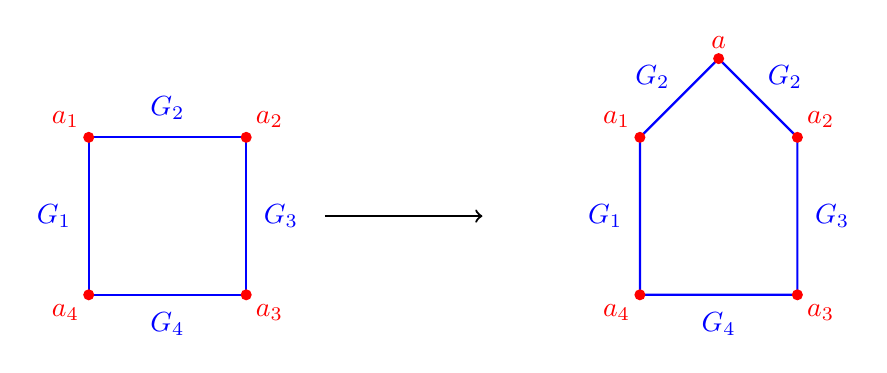
\begin{tikzpicture}
 
    % Left side (Square)
    % Define points for square
    \coordinate (a1) at (0, 0);
    \coordinate (a2) at (2, 0);
    \coordinate (a3) at (2, -2);
    \coordinate (a4) at (0, -2);

    % Draw square with labels
    \draw[thick, blue] (a1) -- (a2) -- (a3) -- (a4) -- cycle;
    \fill[red] (a1) circle (2pt) node[above left] {$a_1$};
    \fill[red] (a2) circle (2pt) node[above right] {$a_2$};
    \fill[red] (a3) circle (2pt) node[below right] {$a_3$};
    \fill[red] (a4) circle (2pt) node[below left] {$a_4$};
    
    % Label edges
    \node[above, blue] at (1, 0.1) {$G_2$};
    \node[right, blue] at (2.1, -1) {$G_3$};
    \node[below, blue] at (1, -2.1) {$G_4$};
    \node[left, blue] at (-0.1, -1) {$G_1$};

    % Arrow between diagrams (shifted right)
    \draw[->, thick] (3, -1) -- (5, -1);

    % Right side (Pentagon, shifted right)
    % Define points for pentagon
    \coordinate (b1) at (7, 0);
    \coordinate (b2) at (9, 0);
    \coordinate (b3) at (9, -2);
    \coordinate (b4) at (7, -2);
    \coordinate (a) at (8, 1);  % New point at top

    % Draw pentagon with labels
    \draw[thick, blue] (b1) -- (a) -- (b2) -- (b3) -- (b4) -- cycle;
    \fill[red] (b1) circle (2pt) node[above left] {$a_1$};
    \fill[red] (b2) circle (2pt) node[above right] {$a_2$};
    \fill[red] (b3) circle (2pt) node[below right] {$a_3$};
    \fill[red] (b4) circle (2pt) node[below left] {$a_4$};
    \fill[red] (a) circle (2pt) node[above] {$a$};

    % Label edges
    \node[above left, blue] at (7.5, 0.5) {$G_2$};
    \node[above right, blue] at (8.5, 0.5) {$G_2$};
    \node[right, blue] at (9.1, -1) {$G_3$};
    \node[below, blue] at (8, -2.1) {$G_4$};
    \node[left, blue] at (6.9, -1) {$G_1$};  % New edge label for left side

      
   \end{tikzpicture}     
   \caption{Illustration of operator 
${\cal G}^{(a)}_{k}$}
        \label{fig:op_gka}
 \end{figure}

 \noindent 
 \emph{2.}  For $1 \le k < l \le n$, we define the cut and glue operator ${\cal G}^{(a), L}_{k, l}$ as follows: ${\cal G}^{(a), L}_{k, l} \circ {\cal L}_{t, \boldsymbol{\sigma}, \textbf{a}}$ (where $L$ stands for "left") is the $G$ loop obtained by cutting the $k$-th and $l$-th $G$ edges $G_t(\sigma_k)$ and $G_t(\sigma_l)$ (creating four end points and two ``chains"), then gluing the two new ends of the chain that contains $E_{a_n}$ and inserting a new $E_a$ at the gluing point. The length of the new loop will be $k + n - l + 1$. For example in figure \ref{fig:op_gLeft}, for $n=5$:
    $$
    {\cal G}^{(a), L}_{3, 5} \circ {\cal L}_{t, \boldsymbol{\sigma}, \textbf{a}} = {\cal L}_{t, \; \boldsymbol{\sigma}', \textbf{a}'}, \quad 
     {\cal G}^{(a), L}_{3, 5}\circ\left(\boldsymbol{\sigma}, \textbf{a}\right)=\left(\boldsymbol{\sigma}', \textbf{a}'\right)
    $$
and 
$$ \boldsymbol{\sigma}=(\sigma_1,\sigma_2,\sigma_3,\sigma_4,\sigma_5),\quad 
   \textbf{a}= (a_1,a_2,a_3,a_4,a_5),\quad \boldsymbol{\sigma}' = (\sigma_1, \sigma_2, \sigma_3, \sigma_5), \quad \textbf{a}' = (a_1, a_2, a, a_5)
$$
  Notice that $a_n$ is always in ${\cal G}^{(a), L}_{k, l}$ for any $k, l$, and $a_1$ is in it for any $k\ge 2$.  

    
    \begin{figure}[ht]
        \centering
         \scalebox{0.8}{
       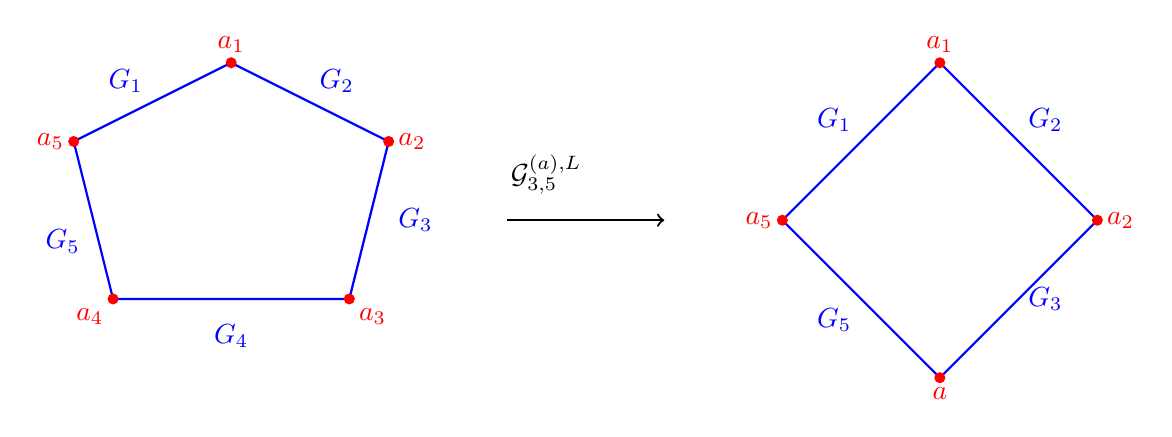
\begin{tikzpicture}
        % Left side (Pentagon)
        % Define points for pentagon
        \coordinate (a1) at (0, 2);
        \coordinate (a2) at (2, 1);
        \coordinate (a3) at (1.5, -1);
        \coordinate (a4) at (-1.5, -1);
        \coordinate (a5) at (-2, 1);

        % Draw pentagon with labels
        \draw[thick, blue] (a1) -- (a2) -- (a3) -- (a4) -- (a5) -- cycle;
        \fill[red] (a1) circle (2pt) node[above] {$a_1$};
        \fill[red] (a2) circle (2pt) node[right] {$a_2$};
        \fill[red] (a3) circle (2pt) node[below right] {$a_3$};
        \fill[red] (a4) circle (2pt) node[below left] {$a_4$};
        \fill[red] (a5) circle (2pt) node[left] {$a_5$};

        % Label edges
        \node[above right, blue] at (1, 1.5) {$G_2$};
        \node[right, blue] at (2, 0) {$G_3$};
        \node[below, blue] at (0, -1.2) {$G_4$};
        \node[below left, blue] at (-1.8, 0) {$G_5$};
        \node[above left, blue] at (-1, 1.5) {$G_1$};

        % Arrow between diagrams
        \draw[->, thick] (3.5, 0) -- (5.5, 0);
        \node[above] at (4, 0.2) {$ {\cal G}^{(a),L}_{3,5}$};

        % Right side (Diamond shape with four points)
        % Define points for diamond shape
        \coordinate (b1) at (9, 2);     % Top
        \coordinate (b2) at (11, 0);     % Right
        \coordinate (a) at (9, -2);     % Bottom (new point a)
        \coordinate (b5) at (7, 0);     % Left

        % Draw diamond shape
        \draw[thick, blue] (b1) -- (b2) -- (a) -- (b5) -- cycle;
        
        % Fill and label points
        \fill[red] (b1) circle (2pt) node[above] {$a_1$};
        \fill[red] (b2) circle (2pt) node[right] {$a_2$};
        \fill[red] (a) circle (2pt) node[below] {$a$};
        \fill[red] (b5) circle (2pt) node[left] {$a_5$};

        % Label edges
        \node[above right, blue] at (10, 1) {$G_2$};
        \node[right, blue] at (10, -1) {$G_3$};
        \node[below left, blue] at (8, -1) {$G_5$};
        \node[above left, blue] at (8, 1) {$G_1$};
    \end{tikzpicture}
    }
        \caption{Illustration of operator ${\cal G}^{(a), L}_{k, l}$}
        \label{fig:op_gLeft}
    \end{figure}

  \noindent 
 \emph{3.} For $1 \le k < l \le n$, we define the cut-and-glue operator ${\cal G}^{(a), R}_{k, l}$ (where $R$ stands for "right") analogously to ${\cal G}^{(a), L}_{k, l}$, except that we glue the two new ends of the chain that does not contain $E_{a_n}$. The length of the new loop is $l-k+1$. For example, in Figure \ref{fig:op_gRight}, for $n=5$:
      $$
    {\cal G}^{(a), R}_{3, 5} \circ {\cal L}_{t, \boldsymbol{\sigma}, \textbf{a}} = {\cal L}_{t, \; \boldsymbol{\sigma}', \textbf{a}'}, \quad 
     {\cal G}^{(a), R}_{3, 5}\circ\left(\boldsymbol{\sigma}, \textbf{a}\right)=\left(\boldsymbol{\sigma}', \textbf{a}'\right)
    $$
   and  $$
  \boldsymbol{\sigma}=(\sigma_1,\sigma_2,\sigma_3,\sigma_4,\sigma_5),\quad 
   \textbf{a}= (a_1,a_2,a_3,a_4,a_5),\quad \quad   \boldsymbol{\sigma}' = (\sigma_3, \sigma_4, \sigma_5), \quad \textbf{a}' = (a_3, a_4, a)
    $$
    \begin{figure}[ht]
        \centering
       \scalebox{0.8}{  % Scale down to 80%
    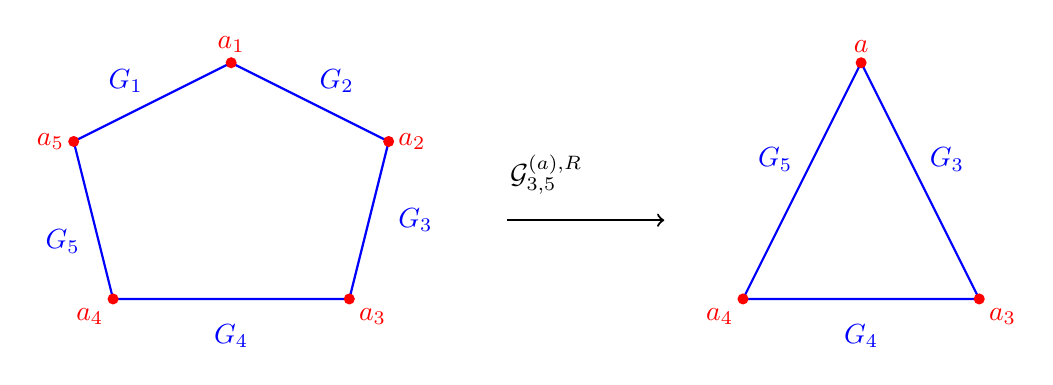
\begin{tikzpicture}
        % Left side (Pentagon)
        % Define points for pentagon
        \coordinate (a1) at (0, 2);
        \coordinate (a2) at (2, 1);
        \coordinate (a3) at (1.5, -1);
        \coordinate (a4) at (-1.5, -1);
        \coordinate (a5) at (-2, 1);

        % Draw pentagon with labels
        \draw[thick, blue] (a1) -- (a2) -- (a3) -- (a4) -- (a5) -- cycle;
        \fill[red] (a1) circle (2pt) node[above] {$a_1$};
        \fill[red] (a2) circle (2pt) node[right] {$a_2$};
        \fill[red] (a3) circle (2pt) node[below right] {$a_3$};
        \fill[red] (a4) circle (2pt) node[below left] {$a_4$};
        \fill[red] (a5) circle (2pt) node[left] {$a_5$};

        % Label edges
        \node[above right, blue] at (1, 1.5) {$G_2$};
        \node[right, blue] at (2, 0) {$G_3$};
        \node[below, blue] at (0, -1.2) {$G_4$};
        \node[below left, blue] at (-1.8, 0) {$G_5$};
        \node[above left, blue] at (-1, 1.5) {$G_1$};

        % Arrow between diagrams
        \draw[->, thick] (3.5, 0) -- (5.5, 0);
        \node[above] at (4, 0.2) {${\cal G}^{(a),R}_{3,5}$};

        % Right side (Triangle)
        % Define points for triangle
        \coordinate (a) at (8, 2);      % Top point (a)
        \coordinate (a3) at (9.5, -1);  % Bottom right point (a3)
        \coordinate (a4) at (6.5, -1);  % Bottom left point (a4)

        % Draw triangle with labels
        \draw[thick, blue] (a) -- (a3) -- (a4) -- cycle;

        % Fill and label points
        \fill[red] (a) circle (2pt) node[above] {$a$};
        \fill[red] (a3) circle (2pt) node[below right] {$a_3$};
        \fill[red] (a4) circle (2pt) node[below left] {$a_4$};

        % Label edges
        \node[above right, blue] at (8.75, 0.5) {$G_3$};
        \node[below, blue] at (8, -1.2) {$G_4$};
        \node[above left, blue] at (7.25, 0.5) {$G_5$};

    \end{tikzpicture}
    }  % End of scalebox
         \caption{Illustration of operator ${\cal G}^{(a), R}_{k, l}$}
        \label{fig:op_gRight}
    \end{figure}
Notice that the loop containing  the index $a_n$ is the left loop, the other is the right loop.  
\end{definition}


Denote by  
$\partial_{(i,j)}:=\partial_{H_t(i,j)},\quad 1\le i\le j\le N$. By  It\^o's formula, we have the following lemma. 
We will use the convention that $\textbf{a} = (a_1 \ldots a_n)$  is a vector while $a$ will be used as an index independent of $\textbf{a} $. We will use this convention throughout the paper.  
 
%

\begin{lemma}[The loop hierarchy] \label{lem:SE_basic}
The $G$-loops satisfy  the loop hierarchy 
\begin{align}\label{eq:mainStoflow}
    d\mathcal{L}_{t, \boldsymbol{\sigma}, \textbf{a}} =& 
    \mathcal{E}^{(M)}_{t, \boldsymbol{\sigma}, \textbf{a}} 
    +
    \mathcal{E}^{(\widetilde{G})}_{t, \boldsymbol{\sigma}, \textbf{a}}\,dt
    +
   W\cdot \sum_{1 \le k < l \le n} \sum_{a, b} \left( \mathcal{G}^{(a), L}_{k, l} \circ \mathcal{L}_{t, \boldsymbol{\sigma}, \textbf{a}} \right) S^{(B)}_{ab} \left( \mathcal{G}^{(b), R}_{k, l} \circ \mathcal{L}_{t, \boldsymbol{\sigma}, \textbf{a}} \right) dt, 
\end{align}
 where the martingale term and the $\widetilde{G}$ terms are defined by 
 \begin{align} \label{def_Edif}
\mathcal{E}^{(M)}_{t, \boldsymbol{\sigma}, \textbf{a}} := & \sum_{\alpha=(i,j)} 
  \left( \partial_{  \alpha} \; {\cal L}_{t, \boldsymbol{\sigma}, \textbf{a}}  \right)
 \cdot \left(S _\alpha\right)^{1/2} \cdot
  \mathrm{d} \left({\cal B}_t\right)_{\alpha} \\\label{def_EwtG}
  \mathcal{E}^{(\widetilde{G})}_{t, \boldsymbol{\sigma}, \textbf{a}}:= &   {W}\cdot \sum_{1 \le k \le n} \sum_{a, b} \; 
 \left \langle \widetilde{G}_t(\sigma_k) E_a \right\rangle
  \cdot S^{(B)}_{ab} \cdot
  \left( {\cal G}^{(b)}_{k} \circ {\cal L}_{t, \boldsymbol{\sigma}, \textbf{a}} \right)  ,\quad \quad \widetilde{G}_t = G_t - m
\end{align}
Notice that the factor $W$ arises because $E_a$ contains a factor $W^{-1}$.

  \end{lemma}
  


 
In order to solve this hierarchy, we introduce the primitive loops, denoted by $\cal K$. 

\begin{definition}[The primitive equation]\label{Def_Ktza}
For 
$$
\boldsymbol{\sigma}=(\sigma_1, \sigma_2, \cdots \sigma_n),\quad 
\boldsymbol{a}=(a_1, a_2, \cdots a_n)
,\quad \sigma_i \in \{+,-\}, \quad
a_i\in \mathbb Z_L, \quad 1\le i\le n
$$
and  $m(\sigma)$ defined in \eqref{def_mtzk}, we define  ${\cal K}_{t, \boldsymbol{\sigma}, \textbf{a}}$ to be the unique solution to the equation 
 \begin{align}\label{pro_dyncalK}
       \frac{d}{dt}\,{\cal K}_{t, \boldsymbol{\sigma}, \textbf{a}} 
       =  
       {W}\cdot  \sum_{1 \le k < l \le n} \sum_{a, b} \; \left( {\cal G}^{(a), L}_{k, l} \circ {\cal K}_{t, \boldsymbol{\sigma}, \textbf{a}} \right) S^{(B)}_{ab} \left( {\cal G}^{(b), R}_{k, l} \circ {\cal K}_{t, \boldsymbol{\sigma}, \textbf{a}} \right)  
    \end{align}
with the initial value 
$$
    {\cal K}_{0, \boldsymbol{\sigma}, \textbf{a}} =  {W^{-n+1}} \cdot \prod_{k=1}^n m (\sigma_k) \cdot \textbf{1}(a_1 = a_2 = \cdots = a_n).
$$
Here we define the ${\cal G}$ operator acting on ${\cal K}$ in the same way as it acts on ${\cal L}$,  i.e.,  
  \be\label{calGonIND}
     {\cal G}^{(a),\,L }_{k,l}  \circ {\cal K}_{t, \boldsymbol{\sigma}, \textbf{a}} = {\cal K}_{t, \; {\cal G}^{(a),\,L }_{k,l}  (\boldsymbol{\sigma}, \textbf{a})}  \quad \forall t, k, \boldsymbol{\sigma}, \textbf{a},   
       \ee
and similarly for  ${\cal G}^{(b),\, R }_{k,l}$. 
For the special case $n=1$, we define % the r.h.s. of \eqref{pro_dyncalK} is zero. Therefore for $n=1$ case
$
{\cal K}_{t,\,+,\, a}=m,\quad {\cal K}_{t,\,-,\, a}=\overline m$ for $0\le t\le 1$. 
\end{definition}

Notice that  ${\cal L}_{t, \boldsymbol{\sigma}, \textbf{a}}$ is an $n$-loop and $\partial_{  \alpha} \; {\cal L}$ is a product of $n+1$ resolvents. Hence  \eqref{eq:mainStoflow} is not an equation, but  a hierarchy. However, the  lengths of ${\cal G}^{(a), L}_{k, l} \circ {\cal K}_{t, \boldsymbol{\sigma}, \textbf{a}}$ and ${\cal G}^{(a), R}_{k, l} \circ {\cal K}_{t, \boldsymbol{\sigma}, \textbf{a}}$ are no greater than the  length of ${\cal K}_{t, \boldsymbol{\sigma}, \textbf{a}}$. Therefore, 
the system of equations for $\cal K$ can be solved inductively. 
 In the next section, we will provide an explicit  solution to the primitive equation.  




%Conceptually, the main focus in these papers lies in the  insertion operators being  traceless since the tracial part, being a constant,  is rather simple. 



 

Earlier mean-field work considered traces of products of resolvents with operator insertions
\cite{CipolloniErdosSchroder2022OptimalMultiResolvent,CipolloniErdosSchroder2022RankUniform}.
The evolution of these traces under a ``renormalized'' Ornstein--Uhlenbeck process was studied in connection with the edge spectral statistics of Wigner matrices \cite{CipolloniErdosHenheik2023EdgeETH}. The resulting flow equations (see (4.5) of \cite{CipolloniErdosHenheik2023EdgeETH}) are analogous to the loop hierarchy \eqref{eq:mainStoflow}. In the mean-field setting, the leading terms of these traces are explicit expressions involving the insertion operators.
After a suitable transformation, these leading terms satisfy a quadratic recursive relation analogous to \eqref{pro_dyncalK}, with $S^{(B)}$ replaced by a scalar corresponding to the one-block case and the primitive loop on the left-hand side replaced by the corresponding observable with multiple operator insertions.

%Despite this structural similarity, the resulting recursion in \cite{CipolloniErdosHenheik2023EdgeETH} is not itself an evolution equation in the usual sense, which is a fundamental feature of \eqref{pro_dyncalK}.

Conceptually, the works \cite{CipolloniErdosHenheik2023EdgeETH,CipolloniErdosSchroder2022OptimalMultiResolvent,CipolloniErdosSchroder2022RankUniform} emphasize operator insertions, whereas the band structure enters only through the degenerate one-block setting, represented by a $1\times1$ covariance matrix. In contrast, the dependence on the band structure and the analysis of the primitive equation are central to the present work. For a more detailed discussion of the mean-field setting, we refer the reader to the original articles, especially \cite{CipolloniErdosHenheik2023EdgeETH}.




%\cite{CipolloniErdosXu2023Extremal,CipolloniErdosSchroder2024MesoscopicNonHermitian,stone2024randommatrixmodelquantum}. 



\subsection{Propagator \texorpdfstring{$\Theta_\xi^{(B)}$}{Theta} and examples of \texorpdfstring{${\cal K}$}{ K}}
 
 \begin{definition}[Propagator $\Theta_\xi^{(B)}$]\label{def_Theta}
Define the propagator  $\Theta_\xi^{(B)}$ by 
\begin{equation}\label{def_Thxi}
    \Theta^{(B)}_\xi := \frac{1}{1 - \xi \cdot S^{(B)}}, \quad \xi \in \mathbb{C}, \quad |\xi| < 1
\end{equation}
where the superscript $B$  indicates the block level matrix. Clearly, 
\begin{equation}\label{deri_Thxi}
    \partial_\xi \Theta^{(B)}_\xi = \Theta^{(B)}_\xi \cdot S^{(B)} \cdot \Theta^{(B)}_\xi.
\end{equation}
By definition, $\Theta_\xi^{(B)}$ is an \(L \times L\) matrix at the block level. We will 
omit the superscript \((B)\) for the rest of this paper. We remind the reader that $\Theta$
is often used to denote the \(N \times N\) matrix 
 \((1 - \xi S)^{-1}\) in the literature.   In this paper,  $\Theta_\xi= \Theta_\xi^{(B)}$.
The following  three special  cases are often used in this paper: 
\[
\Theta^{(B)}_{t m^2}, \quad \Theta^{(B)}_{t \bar{m}^2}, \quad \text{and} \quad \Theta^{(B)}_{t |m|^2} = \Theta^{(B)}_{t}.
\]
Here we have used \(|m| = |m^{(E)}|=1\) in our setting. 


\end{definition}

Here we state several properties of $ \Theta^{(B)}$, whose proofs are deferred to the appendix. 
\begin{lemma}\label{lem_propTH}
Suppose that  $\xi\in \mathbb C$   and $|\xi|< 1$.  Define
$$
 \hat{\ell}(\xi) := \min\left((|1-\xi|)^{-1/2},\; L\right),\quad \xi\in \mathbb C 
$$
Then  $\Theta^{(B)}_\xi$ has the following properties:
\begin{enumerate}
    \item Symmetric: $ (\Theta^{(B)}_{\xi})_{xy}= (\Theta^{(B)}_{\xi})_{yx}$.
    \item Translation invariant: $
    (\Theta^{(B)}_{\xi})_{xy}= (\Theta^{(B)}_{\xi})_{x+1, y+1}$.
    \item Commutativity:  
    $$
    \forall \;  \xi, \; \xi' \quad \quad  [S^{(B)}, \Theta^{(B)}_{\xi}]=[\Theta^{(B)}_{\xi\,'}, \Theta^{(B)}_{\xi}]=0
    $$
     \item Exponential decay at length scale $\hat \ell_\xi $:
     \begin{equation}\label{prop:ThfadC}    \left| (\Theta^{(B)}_{\xi})_{xy}\right|\le \frac{C\cdot e^{-c\cdot|x-y|\big/ \hat{\ell}(\xi)}}{|1-\xi|\cdot \hat \ell (\xi)}\,,\quad   \hat{\ell}(\xi) := \min\left((|1-\xi|)^{-1/2},\; L\right)  
     \end{equation}
     
     \item The following  random walk representation of $\Theta_\xi^{(B)}$ converges.
     \begin{align}\nonumber
     \Theta_\xi^{(B)}=\sum_{k=0}^{\infty}\;  \xi^k \cdot \left(S^{(B)}\right)^k
     \end{align} 

     
     \item Derivative bounds. Using the above random-walk representation, we obtain
     \begin{equation}\label{prop:BD1}     
    \left| (\Theta^{(B)}_{\xi})_{x, y}-(\Theta^{(B)}_{\xi})_{x,{y+1}}\right|\prec \frac{1}{\hat{ \ell}(\xi)\cdot |1-\xi|^{1/2} }   
     \end{equation}
 \begin{equation}\label{prop:BD2}     
     \left|2 (\Theta^{(B)}_{\xi})_{x, y}-(\Theta^{(B)}_{\xi})_{x,{y+1}}-(\Theta^{(B)}_{\xi})_{x,{y-1}}\right|\prec  \frac{1}{\|x-y\|+1 } . 
     \end{equation}
\end{enumerate}
\end{lemma}



 The estimate \eqref{prop:ThfadC} shows that $\Theta^{(B)}_{\xi}$ behaves very differently for $\xi = t|m|^2=t$ or $\xi = tm^2$. In the former case, 
$\Theta^{(B)}_{\xi}$ decays exponentially on the length scale $(1-t)^{-1/2}$ (assuming $(1-t)^{-1/2} \ll L$), and we have the $\ell_1$ bound
\[
\sum_b \Big | (\Theta^{(B)}_{\xi})_{ab} \Big | \le C (1-t)^{-1}.
\]
In the case $\xi = tm^2$, $(\Theta^{(B)}_{\xi})_{ab}$ is a short-range kernel with $\ell_1$ norm of order one. We refer to $\Theta^{(B)}_{\xi}$ as a long edge when $\xi=t$, and as a short edge when $\xi=tm^2$ or $\xi=t\bar m^2$.
  

We can  use $\Theta^{(B)}_\xi$ to solve  the primitive equation  $\mathcal{K}_t$ in the special cases $n = 2$ or $ 3$.

\begin{example} %[$\mathcal{K}_{t, \boldsymbol{\sigma}, \textbf{a}}$ for $n=2$]
For  $n = 2$, the  primitive  equation  \eqref{pro_dyncalK} can be written as 
\begin{align}
    \frac{d}{dt}\, \mathcal{K}_{t, \boldsymbol{\sigma}, (a_1, a_2)} = W \cdot \sum_{a, b} \mathcal{K}_{t, \boldsymbol{\sigma}, (a_1, a)} \cdot S^{(B)}_{ab} \cdot \mathcal{K}_{t, \boldsymbol{\sigma}, (b, a_2)}
\end{align}
Denote 
\begin{equation}\label{eq_defm_i}
    m_i = m(\sigma_i).
\end{equation}
Using the propagator  $\Theta^{(B)}$ defined in equation~\eqref{def_Thxi} and the property \eqref{deri_Thxi}, one can easily verify that
\begin{equation}\label{Kn2sol}
    \mathcal{K}_{t, \boldsymbol{\sigma}, \textbf{a}} = W^{-1} m_1 m_2 \left(\Theta^{(B)}_{t \cdot m_1 m_2}\right)_{a_1 a_2}, \quad \textbf{a} = (a_1, a_2)
\end{equation}
%Now for $2$-$G$-loop, the definition of $\cal K$ in Def. \ref{Def_Ktza} shows (here we dropped the superscript ${(E)}$), 
Explicitly, we have 
\begin{equation}\label{Kn2sol2}
{\cal K}_{t,\boldsymbol{\sigma},(a,b)}
=   W^{-1} \cdot \begin{cases}
     |m |^2\left[\left(1- {  t }|m |^2 S^{(B)}\right)^{-1}\right]_{ab} &, \quad \boldsymbol{\sigma}=(+,-)\\
  m^2\left[\left(1- {  t } m^2 S^{(B)}\right)^{-1}\right]_{ab}  &, \quad \boldsymbol{\sigma}=(+,+)    
\end{cases}
\end{equation}


\end{example}


\begin{example}%[${\cal K}_{t, \boldsymbol{\sigma}, \textbf{a}}$ for $n=3$]
For  $n=3$, let 
$\boldsymbol{\sigma}=(\sigma_1, \sigma_2,\sigma_3), \,
\textbf{a}=(a_1, a_2,a_3)$.
Then  \eqref{pro_dyncalK} becomes 
\begin{align}    \frac{d}{dt}\, \mathcal{K}_{t, \boldsymbol{\sigma}, \textbf{a}} = & W \cdot \sum_{b_1, c_1} \mathcal{K}_{t, (\sigma_1,\sigma_2), (a_1, b_1)} \cdot S^{(B)}_{b_1c_1} \cdot \mathcal{K}_{t, \boldsymbol{\sigma}, (c_1, a_2, a_3)}\nonumber \\
    + & W \cdot \sum_{b_2, c_2} \mathcal{K}_{t, (\sigma_2,\sigma_3), (a_2, b_2)} \cdot S^{(B)}_{b_2c_2} \cdot \mathcal{K}_{t, \boldsymbol{\sigma}, (a_1, c_2, a_3)}\nonumber \\
    + & W \cdot \sum_{b_3, c_3} \mathcal{K}_{t, (\sigma_3,\sigma_1), (a_3, b_3)} \cdot S^{(B)}_{b_3c_3} \cdot \mathcal{K}_{t, \boldsymbol{\sigma}, (a_1, a_2, c_3)} \nonumber
\end{align}
Using \eqref{Kn2sol}, we can rewrite it as 
\begin{align} 
    \frac{d}{dt}\, \mathcal{K}_{t, \boldsymbol{\sigma}, \textbf{a}} = &  \sum_{  c_1} \left( m_1m_2\Theta^{(B)}_{tm_1m_2} \cdot S^{(B)}\right)_{a_1c_1} \cdot \mathcal{K}_{t, \boldsymbol{\sigma}, (c_1, a_2, a_3)}\nonumber \\
    + & \sum_{  c_2} \left(m_2m_3 \Theta^{(B)}_{tm_2m_3} \cdot S^{(B)}\right)_{a_2c_2}  \cdot \mathcal{K}_{t, \boldsymbol{\sigma}, (a_1, c_2, a_3)}\nonumber \\
   + & \sum_{  c_3} \left( m_3m_1\Theta^{(B)}_{tm_3m_1} \cdot S^{(B)}\right)_{a_3c_3}  \cdot \mathcal{K}_{t, \boldsymbol{\sigma}, (a_1, a_2, c_3)} \nonumber
\end{align}
Recall 
$
m_i = m  (\sigma_i)
$ defined in \eqref{eq_defm_i}. Using the propagator  $\Theta^{(B)}$  \eqref{def_Thxi} and  \eqref{deri_Thxi}, one can easily verify that 
$$
{\cal K}_{t, \boldsymbol{\sigma}, \textbf{a}} = \sum_b \left(\Theta^{(B)}_{t \cdot m_1 m_2}\right)_{a_1 b} \left(\Theta^{(B)}_{t \cdot m_2 m_3}\right)_{a_2 b} \left(\Theta^{(B)}_{t \cdot m_3 m_1}\right)_{a_3 b} \cdot W^{-2}\cdot m_1 m_2 m_3, \quad  \textbf{a}= (a_1, a_2,a_3).
$$
Alternatively, it can be expressed as
$$
{\cal K}_{t, \boldsymbol{\sigma}, \textbf{a}} = \sum_{b_1 b_2 b_3} \left(\Theta^{(B)}_{t \cdot m_1 m_2}\right)_{a_1 b_1} \left(\Theta^{(B)}_{t \cdot m_2 m_3}\right)_{a_2 b_2} \left(\Theta^{(B)}_{t \cdot m_3 m_1}\right)_{a_3 b_3} \cdot {\cal K}_{0, \boldsymbol{\sigma}, \textbf{b}}, \quad \textbf{b} = (b_1, b_2, b_3).
$$
\end{example}


In the next section, we will prove in Lemma \ref{Lemma_TRofK} that $\mathcal{K}$ can be expressed as a sum over certain tree graphs. This will be called the tree representation of $\mathcal{K}$. The previous explicit solution for $\mathcal{K}$ in the case $n=3$ will be a special case of this representation. 
Using the primitive equation and the tree representation, we will establish the following estimate \eqref{eq:bcal_k} for $\mathcal{K}$. %   stated in Lemma \ref{ML:Kbound+pi}. 
This estimate in the special case $n=3$ follows from the explicit expression of 
${\cal K}$ and the estimate \eqref{prop:ThfadC}. However, starting from $n=4$, the proof of bound \eqref{eq:bcal_k} requires cancellation among contributions from different graphs in the tree representation of $\mathcal{K}$.
To prove Lemma \ref{ML:Kbound}, we will have to use cancellations among summands in the tree representation. 
This key ingredient is the  sum-zero property,  \eqref{eq:bcal_k_pi}, which serves as a critical input.




\begin{lemma}[An upper bound on ${\cal K}$]\label{ML:Kbound}
Recall $\hat \ell $ defined in \eqref{prop:ThfadC}. 
The  primitive loop ${\cal K}_{t, \boldsymbol{\sigma}, \textbf{a}}$ is bounded by
\begin{equation}\label{eq:bcal_k}
  {\cal K}_{t, \boldsymbol{\sigma}, \textbf{a}}  \prec \left(W \ell_t \cdot \eta_t \right)^{-n+1},\quad  \ell_t :=\hat\ell(t)= \min\left((|1-t|)^{-1/2},\; L\right)       
\end{equation}
\end{lemma}

\bigskip

Finally, we note that for any fixed \(|E| < 2 - \kappa\), it is straightforward to verify that 
 \[
\im z_t = \im z_t^{(E)} = \im m^{(E)} \cdot (1 - t) \sim (1 - t).
\]
 Therefore, the \(\ell(z)\) defined in \eqref{def_ellz} and \(\ell_t\) defined in \eqref{eq:bcal_k} are of the same order, as follows:
 \[
\ell(z_t) \sim \ell_t = \hat{\ell}(t).
\]
Furthermore,  for \(z\), \(t\), and \(E\) satisfying the conditions \eqref{eq:zztE} and \eqref{eq:zztE2}, we have 
 \[
\im z\sim \im z^{(E)}_t,\quad \ell(z) \sim \ell(z^{(E)}_t) \sim \ell_t.
\]
Notice that \(\ell_t\) is just a simpler notation for $\hat{\ell}(t)$. 
% Since these quantities are of  the same order, in the following proof, we will use only \(\ell_t\).  
 





\subsection{Estimates on loops}
 

Our main estimates for the $G$-loops are given in the following lemmas (recall that $\prec$ and $\ell_t$ are defined in Definition \ref{stoch_domination} and \eqref{eq:bcal_k}, respectively).

\begin{lemma}[loop estimates]\label{ML:GLoop}
%Denote the length scale $\ell_t:=\ell(z_t)$.  
For any small constants $\kappa, \tau>0$ and  
$E \in[-2+\kappa, 2-\kappa], \, 0\le t\le 1-N^{-1+\tau}$,  
we have 
\begin{equation}\label{Eq:L-KGt}
 \max_{\boldsymbol{\sigma}, \textbf{a}}\left|{\cal L}_{t, \boldsymbol{\sigma}, \textbf{a}}-{\cal K}_{t, \boldsymbol{\sigma}, \textbf{a}}\right|\prec (W\ell_t\eta_t)^{-n},\quad \eta_t:=\im z_t,  %\quad \ell_t:=\ell(z_t)
\end{equation}
 \begin{equation}\label{Eq:L-KGt2}
\max_{\boldsymbol{\sigma}, \textbf{a}}\left|{\cal L}_{t, \boldsymbol{\sigma}, \textbf{a}} \right|\prec (W\ell_t\eta_t)^{-n+1}. %\quad \eta_t:=\im z_t,\quad \ell_t:=\ell(z_t)
\end{equation}
\end{lemma}

\begin{lemma}[$2$-loop estimate]\label{ML:GLoop_expec}
With the notations and assumptions of the previous lemma, 
the expectation of a $2$-$G$-loop is bounded by  
\begin{equation}\label{Eq:Gtlp_exp}
 \max_{\boldsymbol{\sigma}, \textbf{a}}\left|\mathbb E{\cal L}_{t, \boldsymbol{\sigma}, \textbf{a}}-{\cal K}_{t, \boldsymbol{\sigma}, \textbf{a}}\right|\prec (W\ell_t\eta_t)^{-3}
 ,\quad \eta_t:=\im z_t
\end{equation}
for any choice of  $\boldsymbol{\sigma}\in\{+,-\}^2$.
In case $\boldsymbol{\sigma}=(+,-)$ and $ \textbf{a}=(a_1, a_2)$, 
we have
\begin{equation}\label{Eq:Gdecay}
 \left| {\cal L}_{t, \boldsymbol{\sigma}, \textbf{a}}-{\cal K}_{t, \boldsymbol{\sigma}, \textbf{a}}\right|\prec (W\ell_t\eta_t)^{-2}\exp \left(-\left|\frac{ a_1-a_2 }{\ell_t}\right|^{1/2}\right)+W^{-D}. 
\end{equation}
\end{lemma}
This expectation estimate will be used below in the proofs of Theorems \ref{MR:locSC} and \ref{MR:QDiff}. Together with \eqref{Gmt1/2Gm2} and \eqref{Kn2sol}, it yields the expectation bounds \eqref{Meq:QdS1} and \eqref{Meq:QdS2} in Theorem \ref{MR:QDiff}.

\begin{lemma}[Local law for $G_t$]\label{ML:GtLocal}
   With the notations and assumptions of the previous lemma, we have 
\begin{equation}\label{Gt_bound}
 \|G^{(E)}_{t,+}-m^{(E)}\|_{\max}\prec (W\ell_t\eta_t)^{-1/2}.
   \end{equation} 
\end{lemma}
 

\medskip 

\begin{proof}[Proof of Theorems \ref{MR:locSC} and \ref{MR:QDiff}]
For each $z$ in Theorems \ref{MR:locSC} and \ref{MR:QDiff}, Lemma \ref{zztE} shows that there exist $E$ and $t$ satisfying \eqref{eq:zztE} and \eqref{eq:zztE2}, along with the following conditions:
$$
(1-t) \sim \im z_t \sim \im z \geq N^{-1+\tau}, \quad \eta_t \sim \eta, \quad \ell_t \sim \ell(z).
$$
Combining \eqref{mtEmz} and \eqref{GtEGz}, we obtain
\begin{equation}\label{Gmt1/2Gm}
G(z) - m_{sc}(z) \sim  t^{1/2} \left(G_t^{(E)} - m^{(E)}\right).
\end{equation}
This relation holds in distribution.  Thus, the estimate on $G - m$ in \eqref{G_bound} of Theorem \ref{MR:locSC} follows from the estimate on $G_t - m$ in \eqref{Gt_bound} of Lemma \ref{ML:GtLocal}.

Similarly, \eqref{G_bound_ave} follows from \eqref{Eq:L-KGt} for the $1$-$G$-loop, with the definition of $\cal K$ in Definition \ref{Def_Ktza}:
$$
{\cal K}_{t,+,a} = m^{(E)}, \quad 0\le t\le 1. 
$$
Analogously to \eqref{Gmt1/2Gm}, for the $2$-$G$ terms we have:
\begin{equation}\label{Gmt1/2Gm2}
\tr G (z) E_aG (z) E_b \sim t \cdot {\cal L}_{t, (+,+),(a,b)}, \quad \tr G(z) E_aG^\dagger(z)  E_b\sim  t \cdot {\cal L}_{t, (+,-),(a,b)}.
\end{equation}
Using \eqref{Kn2sol} for rank-$2$ $\cal K$, we derive:
\begin{align*}
t \cdot {\cal K}_{t, (+,+),(a,b)}
&= W^{-1} m^2_{sc}(z) \cdot \left(\frac{1}{1 - m^2_{sc}(z) \cdot S^{(B)}}\right)_{ab}, \\
t \cdot {\cal K}_{t, (+,-),(a,b)}
&= W^{-1} |m_{sc}(z)|^2 \cdot \left(\frac{1}{1 - |m_{sc}(z)|^2 \cdot S^{(B)}}\right)_{ab}.
\end{align*}
Therefore, \eqref{Meq:QdW1} and \eqref{Meq:QdW2} in Theorem \ref{MR:QDiff} follow from \eqref{Eq:L-KGt} in the case $n=2$, while \eqref{Meq:QdS1} and \eqref{Meq:QdS2} follow from \eqref{Eq:Gtlp_exp}. 
This completes the proof of Theorems \ref{MR:locSC} and \ref{MR:QDiff}.
 \end{proof}


We remark that there is a  subtle difference between the $2$-loop and the  $T$-observable. 
By definition, the $2$-loop is given by 
$$
{\cal L}_{t, (+,-),(a,b)}= \sum_{i, j}   (G_{t,+})_{ij}  E_a(j) (G_{t,-})_{ji}   E_b(i)=  \sum_{i, j}   |(G_{t,+})_{ij}|^2  E_a(j) E_b(i).
$$
Comparing ${\cal L}_{t, (+,-),(a,b)}$ with the $T$-observable \eqref{T}, we find that there are two averages over indices in the loop observable, but only one average in $T$. Here we neglect the unimportant difference between the $S$ and $E_b$ operators.
While an extra averaging might seem to be insignificant, we remind the reader that in the special case of Wigner matrices,  
\[
N^{-1} \sum_{x y} |G_{x,y}|^2 = (\im z )^{-1}N^{-1}  \sum_x \im G_{xx}. 
\]
The averaging  in the $x$ index is critical for the local law of  Wigner matrices asserting that   the fluctuation of $N^{-1} \tr G$ is one order of magnitude smaller than that of $G_{xx}$.  For similar reasons, our results for $2$-loop will not hold for the $T$ observable \eqref{T}.

 
\noindent 
\textbf{$G$-chains.}
The loop observables discussed above naturally lead to the following $G$-chains, which form a more general class of observables. For
\[
\boldsymbol{\sigma}
   =(\sigma_1,\ldots,\sigma_n)\in\{+,-\}^n,
\qquad
\mathbf a=(a_1,\ldots,a_{n-1})\in\mathbb Z_L^{n-1},
\]
define the G-chain 
\begin{equation*} 
\mathcal C_{t,\boldsymbol{\sigma},\mathbf a}
:=
G_t(\sigma_1)E_{a_1}G_t(\sigma_2)E_{a_2}
\cdots E_{a_{n-1}}G_t(\sigma_n).
\end{equation*}
The quantity $\mathcal C_{t,\boldsymbol{\sigma},\mathbf a}$ is an $N\times N$ matrix, whereas the loop observable $\mathcal L_{t,\boldsymbol{\sigma},\mathbf a}$ is a scalar.
Under the assumptions of Lemma~\ref{ML:GLoop}, for each fixed $n\in\mathbb N$, the diagonal and off-diagonal entries of a $G$-chain satisfy
\begin{align*} 
\max_{\boldsymbol{\sigma}\in\{+,-\}^n}
\max_{\mathbf a\in\mathbb Z_L^{n-1}}
\max_i
\left|
  \bigl(\mathcal C_{t,\boldsymbol{\sigma},\mathbf a}\bigr)_{ii}
\right|
&\prec
  (W\ell_t\eta_t)^{-n+1},
\\ 
\max_{\boldsymbol{\sigma}\in\{+,-\}^n}
\max_{\mathbf a\in\mathbb Z_L^{n-1}}
\max_{i\ne j}
\left|
  \bigl(\mathcal C_{t,\boldsymbol{\sigma},\mathbf a}\bigr)_{ij}
\right|
&\prec
  (W\ell_t\eta_t)^{-n+1/2}.
\end{align*}
These estimates, which parallel the loop estimates in Lemma~\ref{ML:GLoop}, are proved in Lemma~\ref{lem_GbEXP_n2} of Appendix~\ref{sec:Gchains}.

The exponents in the above estimates are compatible with those in Lemma~\ref{ML:GLoop} and are expected to be optimal.
%at the level of uniform power counting. 
%For general $n\ge 2$,
%the same powers are predicted by closing a chain into a loop and using
%the loop estimates in Lemma~\ref{ML:GLoop}. 
However, these bounds need not be sharp for every choice of charges and block indices, because additional cancellations or spatial separation may yield stronger estimates in some configurations.

The main results of this paper require only loop observables because of the special block structure
$S=S^{(B)}\otimes S_W$. In this setting, the block-averaged loop observables form a closed hierarchy. For a general variance profile, this closure is no longer available: the evolution equations for loops also involve chains with diagonal insertions determined by the variance profile.
The hierarchy must then be enlarged to a coupled loop--chain hierarchy, and the chains must be estimated in terms of loop observables. An extension of the above estimates has recently been used for power-law random band matrices with general variance profiles; see
\cite[Section~9]{FanYangYin2026PowerLawRBM}. This development illustrates how the loop-flow strategy can be adapted to general variance profiles and explains the importance of the chain estimates proved in Appendix~\ref{sec:Gchains}.

 

\subsection{Proof strategy for the main lemmas}

We now outline the proofs of Lemmas \ref{ML:GLoop}, \ref{ML:GLoop_expec} and \ref{ML:GtLocal}.
By Definitions \ref{Def:G_loop} and \ref{Def_Ktza},   
$$
G_{0}(+)=m\cdot I_{N\times N}, \quad {\cal L}_{0, \boldsymbol{\sigma},\textbf{a}}= {\cal K}_{0, \boldsymbol{\sigma},\textbf{a}},\quad \forall \; \boldsymbol{\sigma},\textbf{a}, 
$$
where $I_{N\times N}$ is the identity matrix. It is easy to check that  
\begin{align}\label{ini)bigasya}
    \hbox{    Lemmas \ref{ML:GLoop}, \ref{ML:GLoop_expec} and \ref{ML:GtLocal} hold at  $t=0$ with no error.}
\end{align}
For $t>0$, we will prove the following theorem.


\begin{theorem}\label{lem:main_ind} Fix $E$ and $s\in[0,1]$, with $|E|\le 2-\kappa$, and assume that Lemmas \ref{ML:GLoop}, \ref{ML:GLoop_expec}, and \ref{ML:GtLocal} hold at time $s$, namely, %with $\eta_s:=\im z_s,\quad \ell_s:=\ell(z_s)$,
for $1 \le n\in \mathbb N$ and large $D>0$, 
\begin{align}\label{Eq:L-KGt+IND}
 \max_{\boldsymbol{\sigma}, \textbf{a}}\left|{\cal L}_{s, \boldsymbol{\sigma}, \textbf{a}}-{\cal K}_{s, \boldsymbol{\sigma}, \textbf{a}}\right|&\prec (W\ell_s\eta_s)^{-n}  
\\\label{Eq:Gdecay+IND}
 \left| {\cal L}_{s, \boldsymbol{\sigma}, \textbf{a}}-{\cal K}_{s, \boldsymbol{\sigma}, \textbf{a}}\right|&\prec (W\ell_s\eta_s)^{-2}\exp \left(- \left|\frac{ a_1-a_2 }{\ell_s}\right|^{1/2}\right)+W^{-D} , \quad \boldsymbol{\sigma}=(+,-)
\\\label{Gt_bound+IND}
 \|G^{(E)}_{s ,+}-m^{(E)}\|_{\max} & \prec (W\ell_s\eta_s)^{-1/2},
 \\\label{Eq:Gtlp_exp+IND}
 \max_{\boldsymbol{\sigma}, \textbf{a}}\left|\mathbb E{\cal L}_{s, \boldsymbol{\sigma}, \textbf{a}}-{\cal K}_{s, \boldsymbol{\sigma}, \textbf{a}}\right|&\prec (W\ell_s\eta_s)^{-3},\quad  \forall\; \boldsymbol{\sigma}\in \{+,-\}^2.
\end{align}
 Then for any $t>s$ with $t\le 1-N^{-1+\tau}$ for some fixed $\tau>0$, satisfying 
\begin{equation}\label{con_st_ind}
    (W\ell_t\eta_t)^{-1}\le \left(\frac{1-t}{1-s}\right)^{30}
\end{equation}
%Here $2024$ is just for a large number, the exact value will not affect our final results) then
we have that 
\eqref{Eq:L-KGt+IND}, \eqref{Eq:Gtlp_exp+IND}, \eqref{Eq:Gdecay+IND} and \eqref{Gt_bound+IND} hold with $s$  replaced by $t$.   
\end{theorem}

\begin{proof}[Proof of Lemmas \ref{ML:GLoop}, \ref{ML:GLoop_expec},  and \ref{ML:GtLocal}]
For any fixed $\tau$ and  $t \le 1-N^{-1+\tau}$,  choose $\tau'>0$ and $n_0 \in \mathbb N$ such that 
$$
(W\ell_t\eta_t)^{-1}\le  W^{- 30 \tau'} , \quad (1-t) = W^{-n_0 \tau'}
$$
Let 
\[
1-s_{k} = W^{-k \tau'}, \quad k \le n_0, \quad s_{n_0} = t
\]
 
Since  $W\ell_s\eta_s$ is decreasing in  $s\in [0,1]$, we have 
   $$
(W\ell_{s_{k+1}}\eta_{s_{k+1}})^{-1}\le (W\ell_{t}\eta_{t})^{-1}\le W^{- 30\tau'}
\le \left(\frac{1-s_{k}}{1-s_{k+1}}\right)^{-30}
$$
for all $k$ such that  $k+1\le n_0$. 
We can now apply  Theorem  \ref{lem:main_ind} from $s_k$ to $s_{k+1}$ for $k=0$ until $k=n_0-1$ so that the conclusions of  Theorem  \ref{lem:main_ind} hold for  $s_{n_0}=t$.  We have thus proved Lemmas \ref{ML:GLoop}, \ref{ML:GLoop_expec}, and \ref{ML:GtLocal}.  Notice that for any $\tau$ fixed, $n_0$ is a finite number depending on $\tau$.  Thus we have only finitely many iterations. This is important because every time we apply  Theorem  \ref{lem:main_ind} our inequalities deteriorate by a factor 
$N^\varepsilon$. At the end, we will have a factor $N^{n_0 \varepsilon}$ at the time $t$. Since $\varepsilon$ is arbitrarily small, this factor is still harmless for any $\tau$ fixed. 
\end{proof}


 
 
Theorem \ref{lem:main_ind} will be proved in six steps, with their detailed proofs provided in Section \ref{Sec:Stoflo}. Throughout these steps, we assume that the conditions of Theorem \ref{lem:main_ind} are satisfied. In addition, each step builds on the conclusions established in the preceding steps.

\medskip 
\noindent 
\textbf{Step 1}   (A priori loop bounds): The $n$-loop is bounded by 
 \begin{equation}\label{lRB1}
   {\cal L}_{u,\boldsymbol{\sigma}, \textbf{a}}\prec (\ell_u/\ell_s)^{(n-1)}\cdot 
   (W\ell_u\eta_u)^{-n+1},\quad  s\le u\le t.
\end{equation}
Furthermore,  the  weak local law holds in the sense 
\begin{equation}\label{Gtmwc}
    \|G_u-m\|_{\max}\prec  (W\ell_u\eta_u)^{-1/4},\quad s\le u\le t .
\end{equation} 
Here the exponent  is $1/4$ instead of $1/2$  in \eqref{Gt_bound+IND}. 
 




 \bigskip
\noindent 
\textbf{Step 2}  (A priori $2$-loop decay): 
 The following local law holds for $u\in [s,t]$, namely, 
 \begin{equation}\label{Gt_bound_flow}
     \|G_u-m\|_{\max}\prec  (W\ell_u\eta_u)^{-1/2},\quad s\le u\le t.
\end{equation} 
Hence \eqref{Gt_bound+IND} in Theorem \ref{lem:main_ind} holds.  
In addition,  with 
 $\boldsymbol{\sigma}=(+,-)$, we have for any   $s\le u\le t$ and $D>0$ that 
 \begin{equation}\label{Eq:Gdecay_w}
\left| {\cal L}_{u, \boldsymbol{\sigma}, \textbf{a}}-{\cal K}_{u, \boldsymbol{\sigma}, \textbf{a}}\right| \prec \left(\eta_s/\eta_u\right)^4\cdot (W\ell_u\eta_u)^{-2}\exp \left(- \left|\frac{ a_1-a_2 }{\ell_u}\right|^{1/2}\right)+W^{-D} . \quad 
\end{equation}
   \bigskip
 \noindent 
\textbf{Step 3}   (Sharp  loop  bounds): 
 The following sharp estimate on $n$-$G$-loop holds: 
\begin{equation}\label{Eq:LGxb}
\max_{\boldsymbol{\sigma}, \textbf{a}}\left| {\cal L}_{u, \boldsymbol{\sigma}, \textbf{a}} \right|
\prec 
  (W\ell_u\eta_u)^{-n+1} ,\quad \quad s\le u\le t, \quad\forall\, n\in \mathbb N.
\end{equation}


 \bigskip
 \noindent 
\textbf{Step 4}  (A sharp  $\cal L - \cal K$  bound): 
The following sharp estimate on $ {\cal L}_t-{\cal K}_t$ of length $n$ holds: 
\begin{equation}\label{Eq:L-KGt-flow}
 \max_{\boldsymbol{\sigma}, \textbf{a}}\left|{\cal L}_{u, \boldsymbol{\sigma}, \textbf{a}}-{\cal K}_{u, \boldsymbol{\sigma}, \textbf{a}}\right|\prec (W\ell_u\eta_u)^{-n},\quad \quad s\le u\le t, \quad \forall\, n\in \mathbb N
\end{equation}
This implies \eqref{Eq:L-KGt+IND} in Theorem  \ref{lem:main_ind}.



 \bigskip
 \noindent 
\textbf{Step 5}  (A sharp decay bound): For  $ \boldsymbol{\sigma}=(+,-)$,
 \begin{equation}\label{Eq:Gdecay_flow}
\left| {\cal L}_{u, \boldsymbol{\sigma}, \textbf{a}}-{\cal K}_{u, \boldsymbol{\sigma}, \textbf{a}}\right| \prec   (W\ell_u\eta_u)^{-2}\exp \left(- \left|\frac{ a_1-a_2 }{\ell_u}\right|^{1/2}\right)+W^{-D}. 
\end{equation}
The last bound implies \eqref{Eq:Gdecay+IND} in Theorem  \ref{lem:main_ind}.



\bigskip
\noindent 
\textbf{Step 6} (A sharp  $\mathbb E \cal L - \cal K$  bound): 
%In this step, under the assumption of lemma \ref{lem:main_ind},   \eqref{Gt_bound_flow}, \eqref{Eq:Gdecay_flow}  and \eqref{Eq:L-KGt-flow},  we will prove the following bound for $\mathbb E{\cal K-L}$, which implies \eqref{Eq:Gtlp_exp+IND} in lemma \ref{lem:main_ind}. 
%For $2$-$G$-loop, i.e., $\boldsymbol{\sigma}\in\{+,-\}^2$, we have
The following estimate on $2$-$G$-loop with $\boldsymbol{\sigma}\in\{+,-\}^2$ holds: 
\begin{equation}\label{Eq:Gtlp_exp_flow}
 \max_{\boldsymbol{\sigma}, \textbf{a}}\left|\mathbb E{\cal L}_{u, \boldsymbol{\sigma}, \textbf{a}}-{\cal K}_{u, \boldsymbol{\sigma}, \textbf{a}}\right|\prec (W\ell_t\eta_t)^{-3},\quad  
 s \le u \le t, \quad\boldsymbol{\sigma}\in\{+,-\}^2.
\end{equation}
We will use Steps 1-5 to  prove  that \eqref{Eq:L-KGt+IND}, \eqref{Eq:Gdecay+IND}, and \eqref{Gt_bound+IND} of Theorem \ref{lem:main_ind} hold with $s$ replaced by $t$. Here \eqref{Eq:Gtlp_exp+IND} will not be needed for Steps 1-5, i.e.,  Theorem \ref{lem:main_ind}  holds if \eqref{Eq:Gtlp_exp+IND} were removed from both the assumption and statement. 


 

 



 

\subsection{Sum zero properties} %Some heuristics for  the proof of Theorem \ref{lem:main_ind}}
 





 


Recall the loop hierarchy \eqref{eq:mainStoflow} of the $n$-loop  is of the form 
\begin{align}
    d\mathcal{L}_{t, \boldsymbol{\sigma}, \textbf{a}} =&
    \mathcal{E}^{(M)}_{t, \boldsymbol{\sigma}, \textbf{a}} 
    +
    \mathcal{E}^{(\widetilde{G})}_{t, \boldsymbol{\sigma}, \textbf{a}} 
    + \mbox{ quadratic terms} . 
\end{align}
The first two terms are linear in the loops (assuming $\tilde G$ is given) and will be shown to be error terms. The primitive hierarchy drops these two error terms but keeps the quadratic terms.  The  term $  \mathcal{E}^{(\widetilde{G})}_{t, \boldsymbol{\sigma}, \textbf{a}} $  involves an $(n+1)$-loop and the quadratic variation of  $ \mathcal{E}^{(M)}_{t, \boldsymbol{\sigma}, \textbf{a}} $ depends on $2n+2$ loops.  The quadratic term, however,  involves only loops up to length $n$.  Therefore, we can solve the primitive equation starting from $n=1, 2 \ldots$. This procedure clearly cannot be applied to the loop hierarchy. 

It turns out  that both $\mathcal K$ and $\mathcal L$ have similar singularities as $t \to 1$ in the form 
\[
\mathcal{L}  \sim 
\left( 1-t \right)^{-C_n} \sim {\mathcal K },    \quad \im z_t \sim 1-t.
\]
This singularity  at $t \to 1$ is  difficult to control.  It  is a common phenomenon for  quadratic differential equations which  typically  are  unstable under perturbation. Since perturbations of  quadratic differential equations are governed by a linear one, we consider a toy  equation
\[
\partial_t f = 2f - c \cdot t + 1, \quad f(0) = a.
\]
This equation can be solved  explicitly 
\[
f(t)= e^{2 t} \big [a  + \frac 1 2    - \frac c 4    \big ] + \frac  { 2 ct + c-2}  4.
\]
If $a  + \frac 1 2    -  \frac c 4   =0$  then \( f(t) = O(t) \).  The subtle condition 
\[
a  + \frac 1 2    -  \frac c 4   =0
\]
changes the exponential growth of $f$ to a linear growth!  Without explicit solutions, it is not easy to prove the sub-exponential bound of the last toy equation. In our setting,   \(\mathcal{K}\)-loops can be solved by an explicit  \emph{tree representation  formula} (Lemma~\ref{Lemma_TRofK}) and  the previous subtle condition will be implemented by a \emph{sum-zero property} of the \(\mathcal{K}\)-loops.   We will show that both \(\mathcal{L}\) and  \(\mathcal{K}\)-loops satisfy   Ward's identity  (Lemma~\ref{lem_WI_K}). From these  Ward's identities, 
we will prove a {sum-zero property} for the \(\mathcal{K}\)-loops. 






\subsection{Notations}
Here we summarize  notation used throughout the paper. 
\begin{itemize}
    \item $W$ is the bandwidth, $L$ is the number of blocks, $N=W\times L$
    \item ${\cal I}_a$ is the $a$-th block, $[i]$ is the block where index $i$ is. $E_a$ is the following matrix only supported on ${\cal I}_a$. 
    $$
    i\in {\cal I}_{[i]}, \quad (E_a)_{ij}=W^{-1}\delta_{ij}{\bf 1}(i\in {\cal I}_a)$$
    \item $S\in \mathbb R^{N\times N}$, $S^{(B)}\in \mathbb R^{L\times L}$, $S_W\in \mathbb R^{W\times W}$ are all related to the variances of the matrix entries, and 
    $$
S= S^{(B)}\otimes S_{W}
$$
\item In the proof involving the stochastic flow, we typically omit the superscript $(E)$ for simplicity. As a result, the notations $z_t$, $G_t$, and $m$ are defined as follows:
\[
z_t = z_t^{(E)}, \quad G_t := (\sqrt{t} H - z_t)^{-1}, \quad m = \lim_{\varepsilon \searrow 0} m_{sc}(E + i \varepsilon).
\]
Additionally, we use $G_t$ to denote $(H_t - z_t)^{-1}$, where $H_t$ has the same distribution as $\sqrt{t} H$. The context will make it clear which interpretation of $G_t$ is being applied in the proof.
\item Associated with $z_t$, let $\eta_t=\im z_t$, and define $\ell_t$ by \eqref{eq:bcal_k} as
$$ \ell_t:=\hat \ell(t)=\min(|1-t|^{-1/2}, L)$$
Here $\ell_t\sim \ell(z_t)\sim \ell(z)$ is  the decay  length. 

    \item $\cal L$ is for $G$-loop, $\cal K$ is  for the deterministic partner of $G$-loop,  and $\cal C$ is for $G$-chain. 

    \item The propagator $\Theta_\xi = \Theta^{(B)}_{\xi}$ is defined in Definition \ref{def_Theta}. It is used to explicitly define the solution of $\mathcal{K}$ in Definition \ref{def33}.

    
    \item The $\Xi^{({\cal L})}$, $\Xi^{({\cal L-K})}$, $\Xi^{({\cal C})}$ are ratios between these quantities and their heuristic size.  
    
    \begin{align}
\Xi^{({\cal L})}_{t, m}&:= \max_{\boldsymbol{\sigma}, \textbf{a}} 
\left|{\cal L}_{t, \boldsymbol{\sigma}, \textbf{a}} \right|\cdot \left(W\ell_t \eta_t\right)^{m-1} \cdot {\bf 1}(\boldsymbol{\sigma} \in \{+,-\}^m),
\nonumber \\
\Xi^{({\cal L-K})}_{t, m}&:= \max_{\boldsymbol{\sigma}, \textbf{a}}
\left|{ ({\cal L-K})}_{t, \boldsymbol{\sigma}, \textbf{a}} \right|\cdot \left(W\ell_t \eta_t\right)^{m }\cdot {\bf 1}(\boldsymbol{\sigma} \in \{+,-\}^m) ,
\nonumber \\
\Xi^{({{\cal C},\;diag })}_{t, m} &:= \max_{\boldsymbol{\sigma}, \textbf{a}} \max_i \left|\left({\cal C}^{(m)}_{t, \boldsymbol{\sigma}, \textbf{a}}\right)_{ii}\right| \cdot \left(W\ell_t \eta_t\right)^{m-1} \cdot {\bf 1}(\boldsymbol{\sigma} \in \{+,-\}^m), \nonumber \\
\Xi^{({{\cal C},\;off})}_{t, m} &:= \max_{\boldsymbol{\sigma}, \textbf{a}} \max_{i \neq j}
\left|\left({\cal C}^{(m)}_{t, \boldsymbol{\sigma}, \textbf{a}}\right)_{ij}\right| \cdot \left(W\ell_t \eta_t\right)^{m-1/2} \cdot {\bf 1}(\boldsymbol{\sigma} \in \{+,-\}^m).
\end{align}
\item The operators $\varTheta_{t,\boldsymbol{\sigma}}$ and ${\cal U}_{s, t,\boldsymbol{\sigma}}$ are defined in Def. \ref{DefTHUST} as the linear operators for the integrated loop hierarchy for $\cal L-\cal K$ in Lemma \ref{Sol_CalL}. 
\item  The \(\cal G\) operators, such as \({\cal G}^{(a)}_k\), \({\cal G}^{(a),\,L}_{k,l}\), and \({\cal G}^{(a),\,R}_{k,l}\), are defined in Definition \ref{Def:oper_loop}. These operators represent the cutting and gluing of Loop operators within the loop hierarchy.
 

\item \(\Gamma_{t,\boldsymbol{\sigma}, \textbf{a}}\) represents the tree graph used in the tree representation of \(\cal K\). 
\item  The sets \({\cal F}(\Gamma)\) and \({\cal F}_{\text{long}}(\Gamma)\) correspond to the non-neighboring internal edges and the neighboring long internal edges of $\Gamma$, respectively.

\item \({\cal K}^{(\pi)}\) is defined in Definition \ref{def_Kpi} as the sum of certain tree graphs. 
\item \(\Sigma^{(\pi)}\) is further defined as the self-energy of \({\cal K}^{(\pi)}\) in Definition \ref{def_Kpi}. Certain specific \(\Sigma^{(\pi)}\) exhibit the sum-zero property, as demonstrated in Lemma \ref{lem:SZ}.
 
\item  The \(\cal E\) terms represent the non-leading terms that arise in the (integrated) loop hierarchy \eqref{eq:mainStoflow} and \eqref{int_K-LcalE}. Specifically, \({\cal E}^{(M)}\) and \({\cal E}^{(\widetilde{G})}\) are defined in \eqref{def_Edif} and \eqref{def_EwtG}, respectively. The term \(\mathcal{E}^{((\mathcal{L}-\mathcal{K}) \times (\mathcal{L}-\mathcal{K}))}\) is defined in \eqref{def_ELKLK}. Additionally, \(\left( \mathcal{E} \otimes \mathcal{E} \right)\) and \(\left( \mathcal{E} \otimes \mathcal{E} \right)^{(k)}\) are defined in Definition \ref{def:CALE}.

\item  The \({\cal T}^{(\cal L-\cal K)}_{t}\) is defined as the tail function of \(\cal L - \cal K\) in \eqref{def_WTu}. The \({\cal T}_{t,D}\) represents the deterministic rough tail function, as defined in \eqref{def_WTuD}. 
\item The terms \({\cal J}_{u,D}\) and \(\cal J^*\) are introduced in \eqref{def_Ju} and \eqref{shoellJJ}, respectively, to describe the ratio between \({\cal T}^{(\cal L-\cal K)}_{t}\) and \({\cal T}_{t,D}\).

\item The scale $\ell_t^*$ is defined as $\ell_t^*=(\log W)^{3/2}\ell_t$. In this scale $\Theta_t$ is exponentially small, while ${\cal T}_t$ is not. 

\item The operators \(\cal P\) and \({\cal Q}_t\), along with the function \(\vartheta\), are used to define and construct a sum-zero tensor. Their definitions can be found in Definition \ref{Def:QtPt}.
 

\end{itemize}



\section{Definition and properties of \texorpdfstring{$\cal K$}{K}}\label{Sec:CalK}

The primitive loop ${\cal K}$ has an exact formula in terms of summation over tree graphs which we now present. 

\subsection{Tree representation of \texorpdfstring{${\cal K}_{t, \boldsymbol{\sigma}, \textbf{a}}$}{K}}

\begin{definition}[Canonical partition of polygon]
   \begin{figure}[ht]     \centering
      \scalebox{0.8}{
   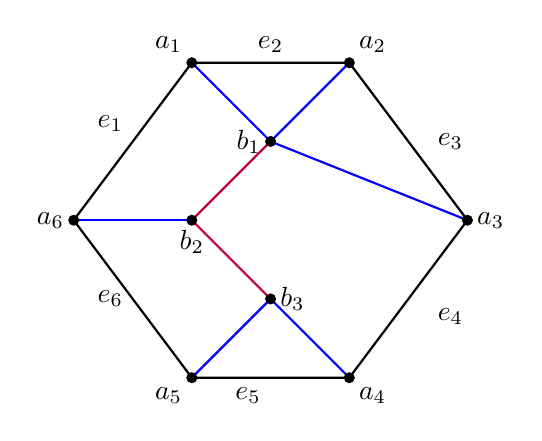
\begin{tikzpicture} 
        % Define vertices of the hexagon
        \coordinate (a1) at (-1, 2);   % Top left
        \coordinate (a2) at (1, 2);   % Top right
        \coordinate (a3) at (2.5, 0); % Middle right
        \coordinate (a4) at (1, -2);  % Bottom right
        \coordinate (a5) at (-1, -2); % Bottom left
        \coordinate (a6) at (-2.5, 0);% Middle left
        \coordinate (b1) at (0, 1);   % Inner point 1
        \coordinate (b2) at (-1, 0); % Inner point 2
        \coordinate (b3) at (0, -1);  % Inner point 3

        % Draw hexagon outline
        \draw[thick, black] (a1) -- (a2) -- (a3) -- (a4) -- (a5) -- (a6) -- cycle;

        % Draw lines from each vertex to inner points
        \draw[thick, blue] (a1) -- (b1) -- (a2); % a1 to b1 to a2
        \draw[thick, blue] (b1) -- (a3) ; %  b1 to a3
        \draw[thick, blue] (a6) -- (b2)  ; % a6 to b2 to a3
        \draw[thick, blue] (a5) -- (b3) -- (a4); % a5 to b3 to a4

        % Draw purple segments for inner lines
        \draw[thick, purple] (b1) -- (b2);
        \draw[thick, purple] (b2) -- (b3);

        % Label outer vertices
        \node[above left] at (a1) {$a_1$};
        \node[above right] at (a2) {$a_2$};
        \node[right] at (a3) {$a_3$};
        \node[below right] at (a4) {$a_4$};
        \node[below left] at (a5) {$a_5$};
        \node[left] at (a6) {$a_6$};

        % Label inner points
        \node[left] at (b1) {$b_1$};
        \node[below] at (b2) {$b_2$};
        \node[ right] at (b3) {$b_3$};
    
        % Label edges of the hexagon
        \node[above] at (0, 2) {$e_2$};         % Edge between a1 and a2
        \node[right] at (2, 1) {$e_3$};      % Edge between a2 and a3
        \node[below right] at (2, -1) {$e_4$}; % Edge between a3 and a4
        \node[below left] at (0, -2) {$e_5$};  % Edge between a4 and a5
        \node[left] at (-1.75 , -1) {$e_6$};     % Edge between a5 and a6
        \node[above left] at (-1.75, 1) {$e_1$}; % Edge between a6 and a1


        % Draw dots at vertices and inner points
        \fill[black] (a1) circle (2pt);
        \fill[black] (a2) circle (2pt);
        \fill[black] (a3) circle (2pt);
        \fill[black] (a4) circle (2pt);
        \fill[black] (a5) circle (2pt);
        \fill[black] (a6) circle (2pt);
        \fill[black] (b1) circle (2pt);
        \fill[black] (b2) circle (2pt);
        \fill[black] (b3) circle (2pt);
    \end{tikzpicture}
    }
    $${\cal V}(\Gamma)=\{ a_1,a_2,a_3,a_4,a_5,a_6,b_1,b_2,b_3 \}$$
    $${\cal E}(\Gamma)=\{\{a_1,b_1\}, \{a_2,b_1\}, 
    \{a_3,b_1\}, \{a_4,b_3\},\{a_5,b_3\},\{a_6,b_2\},\{b_1,b_2\}, \{b_2,b_3\}, \}$$
    $$
    {\cal F}(\Gamma)=\{\{1,4\},\{4,6\}\}$$
      \caption{Illustration of canonical partition of the polygons}
      \label{fig_SPPol}
\end{figure}

Let ${\cal P}_{\textbf{a}}$ be an oriented $n$-gon with ordered vertices $\textbf{a}=(a_1,\ldots,a_n)$, where $a_k$ and $a_{k+1}$ are adjacent. We use the cyclic convention $a_0=a_n$.
The edge $\overline{a_{k-1}a_k}$ is called the $k$-th edge of ${\cal P}_{\textbf{a}}$. In particular, ${\cal P}_{(a,b,c)}\ne {\cal P}_{(b,c,a)}$, because the second edges of these polygons are $\overline{ab}$ and $\overline{bc}$, respectively.
We now define three notions related to partitions of an oriented polygon.

\medskip 
\noindent\textbf{I. Canonical (or standard) partitions.} A partition of ${\cal P}_{\textbf{a}}$ is canonical if and only if
\begin{itemize}
\item Each  sub-region in the partition is also a polygon. 
     \item There is a one-to-one correspondence between the boundary edges of the polygon and its subregions. Each edge $e_k:=\overline{a_{k-1}a_k}$ belongs to exactly one subregion, and each subregion contains exactly one edge $e_k$. We denote the subregion containing $e_i$ by $R_i$.
   \item Each vertex $a_i$  belongs to exactly two regions, i.e.,  $R_i$ and $R_{i+1}$ (with $R_1=R_{n+1}$). 
  
\end{itemize}
%Note that following a canonical partition, the $n$-polygon (i.e., the black edges in Fig. \ref{fig_SPPol}) can be compressed into a zero-area loop along the interior boundaries (i.e., the blue and purple edges in Fig. \ref{fig_SPPol}).

\medskip 
\noindent 
\noindent\textbf{II. Equivalence of canonical partitions.}
Two canonical partitions $P$ and $\widetilde P$ are equivalent if
$$
 P\sim \widetilde{P}\;\iff
\quad \left(\forall\; 1\le  i,j\le n, \quad \quad \quad \; R_{i}\cap R_j=\emptyset \iff
  \widetilde{R}_{i}\cap \widetilde{R}_j=\emptyset \right), 
$$
that is, the corresponding subregions in the two partitions have the same adjacency relations.
We denote by $SP({\cal P}_{\textbf{a}})$ the set of equivalence classes of canonical partitions of ${\cal P}_{\textbf{a}}$:
$$
SP({\cal P}_{\textbf{a}}):=\{[P]: [P] \text{ is an equivalence class of canonical partitions of } {\cal P}_{\textbf{a}}\}.
$$

\medskip 
\noindent\textbf{III. The tree structure of a canonical partition.}
To each equivalence class of canonical partitions of an $n$-gon, we associate a tree obtained by removing the boundary edges of the polygon. We denote the resulting collection, namely, the set of trees of standard partitions, by $TSP({\cal P}_{\textbf{a}})$:
$$
TSP({\cal P}_{\textbf{a}}):=\left\{\Gamma: \Gamma \text{ is the tree associated with } [P]\in SP({\cal P}_{\textbf{a}})\right\}.$$



\end{definition}

{We divide edges of a tree $\Gamma$ into two classes: 1. boundary edges consisting of any edge with a vertex in the polygon. 2. internal edges consisting of the rest.  Finally, polygon edges are those edges in the original polygon. }
 

\begin{lemma}[Classification of canonical partitions]\label{lem_CSP}
Let $\Gamma_\textbf{a}\in TSP({\cal P}_\textbf{a})$ be the tree associated with a canonical partition of the polygon ${\cal P}_{\textbf{a}}$. We call two subregions $R_i$ and $R_j$ in $\Gamma_a$ paired if $R_i\,\cap\,R_j\in {\cal E}(\Gamma_{\textbf{a}})$ and $|i-j|>1 \mod n$, i.e., $R_i$ and $R_j$ are
nonadjacent and share an internal edge.
Denote by ${\cal F}(\Gamma_{\textbf{a}})$ the collection
of non-adjacent pairings of subregions, i.e., 
%the collection of  pairs of subregions in $\Gamma_a$ that are  non-adjacent but sharing an internal edge, i.e., 
\begin{equation}\label{set_csp}
{\cal F}(\Gamma_{\textbf{a}}):=
\Big\{\{i,j\}: |R_i\,\cap\,R_j|\in {\cal E} (\Gamma_{\textbf{a}}),    \quad |i-j|>1 \mod n \Big\}.  
\end{equation}
Here  $\mod n$ implies that $|1- n |= 1$. 
 E.g., for the partition in Fig. \ref{fig_SPPol}, we have ${\cal F}=\{\{1,4\},\{6,4\} \}$. 

Then for  $\Gamma'_\textbf{a}$, $\Gamma_\textbf{a} \in TSP({\cal P}_\textbf{a})$, we have 
$$
\Gamma'_\textbf{a}=\Gamma _\textbf{a}\iff {\cal F}(\Gamma_{\textbf{a}})={\cal F}(\Gamma'_{\textbf{a}})
$$
Furthermore,  we say $\{i,j\}$ and  $\{k,l\}$ (with $i<j$, $k<l$) are crossing pairs if they satisfy 
 $$
 i<k<j<l \quad \text{or} \;  k<i<l<j
 $$
 where the ordering is on $\mathbb Z$ instead of $\mathbb Z_n$. 
 Then we have the following properties 
 \begin{enumerate}
     \item  ${\cal F}(\Gamma_{\textbf{a}})$ contains  {\textit no} crossing pairs.
     \item If ${\cal F}^*$ is a subset of $\left\{\{i, j\}:   | i-j|>1, \mod  \, n\right\}$ and there are {\textit no} crossing pairs in ${\cal F}^*$, then there exists a 
     canonical partition $\Gamma_{\textbf{a}}$ such that  ${\cal F}^*={\cal F}(\Gamma_{\textbf{a}})$.
 \end{enumerate}
\end{lemma}

\begin{proof}[Proof of lemma \ref{lem_CSP}] We prove this lemma by  mathematical induction. First, if ${\cal F}(\Gamma_{\textbf{a}})=\varnothing$, then the tree graph inside must be a star (for $n\ge 3$) as in Figure \ref{fig_star}. 
\begin{figure}[ht]
    \centering
      \scalebox{0.5}{
    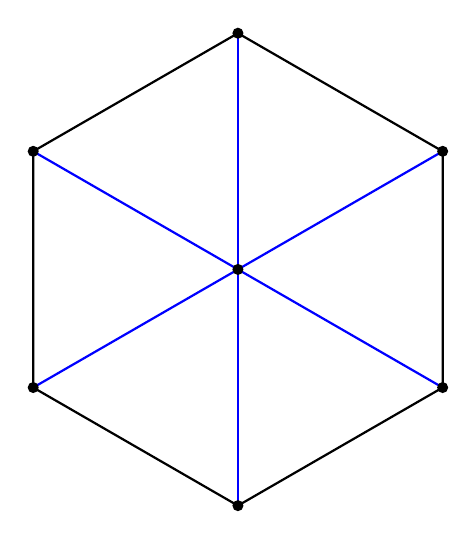
\begin{tikzpicture}
        % Define vertices of the hexagon
        \coordinate (A1) at (0, 3);      % Top
        \coordinate (A2) at (2.6, 1.5);  % Top-right
        \coordinate (A3) at (2.6, -1.5); % Bottom-right
        \coordinate (A4) at (0, -3);     % Bottom
        \coordinate (A5) at (-2.6, -1.5);% Bottom-left
        \coordinate (A6) at (-2.6, 1.5); % Top-left
        \coordinate (Center) at (0, 0);  % Center

        % Draw hexagon outline
        \draw[thick, black] (A1) -- (A2) -- (A3) -- (A4) -- (A5) -- (A6) -- cycle;

        % Draw lines from each vertex to the center
        \draw[thick, blue] (A1) -- (Center);
        \draw[thick, blue] (A2) -- (Center);
        \draw[thick, blue] (A3) -- (Center);
        \draw[thick, blue] (A4) -- (Center);
        \draw[thick, blue] (A5) -- (Center);
        \draw[thick, blue] (A6) -- (Center);

        % Draw dots at vertices and center
        \fill[black] (A1) circle (2pt);
        \fill[black] (A2) circle (2pt);
        \fill[black] (A3) circle (2pt);
        \fill[black] (A4) circle (2pt);
        \fill[black] (A5) circle (2pt);
        \fill[black] (A6) circle (2pt);
        \fill[black] (Center) circle (2pt);

    \end{tikzpicture}
    }
    \caption{Star graph}
    \label{fig_star}
\end{figure}
From now on, we assume that the set in \eqref{set_csp} is nonempty. Assume  for example that $(1,3)\in {\cal F}$. By assumption,  there exists an internal edge connecting $R_1$ and $R_3$. Then the partition can be reduced to two partitions in the smaller polygons:
$$
 {\cal P}_{(a_1,a_2,a)} ,\quad \quad  {\cal P}_{(a_3,a_4,a_5,a_6,b)}. %\quad \color{blue}{fixed}
$$
where $a$ and $b$ are two additional vertices to form two polygons. The rationale for this construction is that once $(1,3)\in {\cal F}$ is given, the original polygon
will be divided into two regions which will not ``communicate". The vertices $a$ and $b$ are added to get back to polygon language. 
Based on this observation, one can easily finish the induction proof.  
$$
 \scalebox{0.8}{\begin{minipage}{0.55\textwidth}
    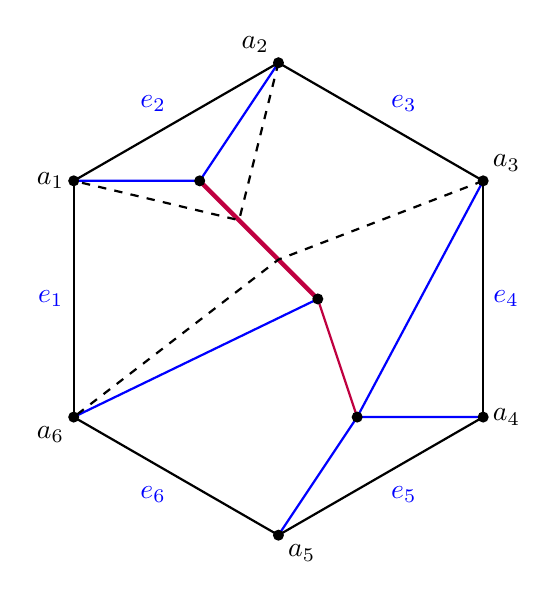
\begin{tikzpicture}
        % Define vertices of the hexagon
        \coordinate (A1) at (0, 3);      % Top
        \coordinate (A2) at (2.6, 1.5);  % Top-right
        \coordinate (A3) at (2.6, -1.5); % Bottom-right
        \coordinate (A4) at (0, -3);     % Bottom
        \coordinate (A5) at (-2.6, -1.5);% Bottom-left
        \coordinate (A6) at (-2.6, 1.5); % Top-left

        % Define inner intersection points
        \coordinate (B1) at (-1, 1.5);          % Near center but higher
        \coordinate (B2) at (-0.5, 1.0);        % Right-center
        \coordinate (B3) at (0, 0.5);       % Bottom-right center
        \coordinate (B4) at (0.5,  0);      % Bottom-left center
        \coordinate (B5) at (1, -1.5);       % Left-center

        % Draw hexagon outline with edge labels
        \draw[thick, black] (A1) -- (A2) node[midway, above right, blue] {$e_3$};
        \draw[thick, black] (A2) -- (A3) node[midway, right, blue] {$e_4$};
        \draw[thick, black] (A3) -- (A4) node[midway, below right, blue] {$e_5$};
        \draw[thick, black] (A4) -- (A5) node[midway, below left, blue] {$e_6$};
        \draw[thick, black] (A5) -- (A6) node[midway, left, blue] {$e_1$};
        \draw[thick, black] (A6) -- (A1) node[midway, above left, blue] {$e_2$};

        % Draw red lines from vertices to the intermediate points
       \draw[thick, blue] (A1) -- (B1) -- (A6);
        \draw[ultra thick, purple] (B1) -- (B4); 
        \draw[thick, blue] (B4) -- (A5);
        \draw[thick, purple] (B4) -- (B5) ;
        \draw[thick, blue] (B5) -- (A2);
        \draw[thick, blue] (A3) -- (B5) -- (A4);

        % Draw dashed lines from vertices to the opposite inner points
        \draw[thick, black, dashed] (A1) -- (B2)--(A6);
        \draw[thick, black, dashed] (A2) -- (B3)--(A5);

        % Draw dots at vertices and inner points
        \fill[black] (A1) circle (2pt);
        \fill[black] (A2) circle (2pt);
        \fill[black] (A3) circle (2pt);
        \fill[black] (A4) circle (2pt);
        \fill[black] (A5) circle (2pt);
        \fill[black] (A6) circle (2pt);
        \fill[black] (B1) circle (2pt);
        %\fill[black] (B2) circle (2pt);
       % \fill[black] (B3) circle (2pt);
        \fill[black] (B4) circle (2pt);
        \fill[black] (B5) circle (2pt);
        
        % Label outer vertices
        % Label outer vertices
        \node[above left] at (A1) {$a_2$};
        \node[above right] at (A2) {$a_3$};
        \node[right] at (A3) {$a_4$};
        \node[below right] at (A4) {$a_5$};
        \node[below left] at (A5) {$a_6$};
        \node[left] at (A6) {$a_1$};
    \end{tikzpicture}
\end{minipage}
\hfill
\begin{minipage}{0.45\textwidth}
    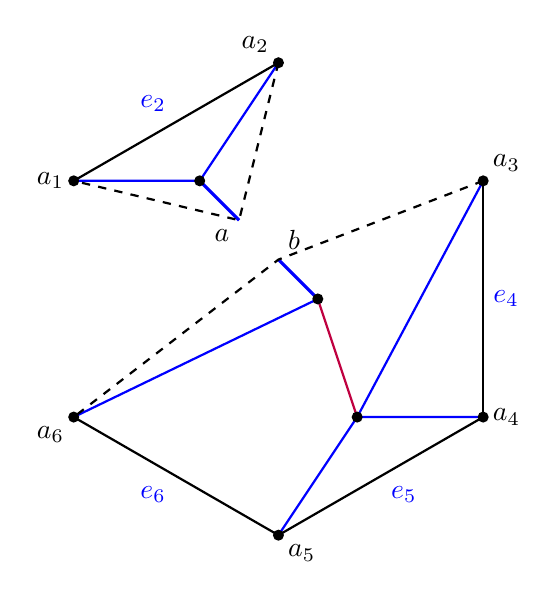
\begin{tikzpicture}
        % Define vertices of the hexagon
        \coordinate (A1) at (0, 3);      % Top
        \coordinate (A2) at (2.6, 1.5);  % Top-right
        \coordinate (A3) at (2.6, -1.5); % Bottom-right
        \coordinate (A4) at (0, -3);     % Bottom
        \coordinate (A5) at (-2.6, -1.5);% Bottom-left
        \coordinate (A6) at (-2.6, 1.5); % Top-left

        % Define inner intersection points
        \coordinate (B1) at (-1, 1.5);          % Near center but higher
        \coordinate (B2) at (-0.5, 1.0);        % Right-center
        \coordinate (B3) at (0, 0.5);       % Bottom-right center
        \coordinate (B4) at (0.5,  0);      % Bottom-left center
        \coordinate (B5) at (1, -1.5);       % Left-center

        % Draw hexagon outline with edge labels
        %\draw[thick, blue] (A1) -- (A2) node[midway, above right, blue] {$e_3$};
        \draw[thick, black] (A2) -- (A3) node[midway, right, blue] {$e_4$};
        \draw[thick, black] (A3) -- (A4) node[midway, below right, blue] {$e_5$};
        \draw[thick, black] (A4) -- (A5) node[midway, below left, blue] {$e_6$};
       % \draw[thick, blue] (A5) -- (A6) node[midway, left, blue] {$e_1$};
        \draw[thick, black] (A6) -- (A1) node[midway, above left, blue] {$e_2$};

        % Draw red lines from vertices to the intermediate points
        \draw[thick, blue] (A1) -- (B1) -- (A6);
        \draw[ very thick, blue] (B1) -- (B2); 
        \draw[ very thick, blue] (B3) -- (B4); 
        \draw[thick, blue] (B4) -- (A5);
        \draw[thick, purple] (B4) -- (B5) ;
        \draw[thick, blue] (B5) -- (A2);
        \draw[thick, blue] (A3) -- (B5) -- (A4);

        % Draw dashed lines from vertices to the opposite inner points
        \draw[thick, black, dashed] (A1) -- (B2)--(A6);
        \draw[thick, black, dashed] (A2) -- (B3)--(A5);

        % Draw dots at vertices and inner points
        \fill[black] (A1) circle (2pt);
        \fill[black] (A2) circle (2pt);
        \fill[black] (A3) circle (2pt);
        \fill[black] (A4) circle (2pt);
        \fill[black] (A5) circle (2pt);
        \fill[black] (A6) circle (2pt);
        \fill[black] (B1) circle (2pt);
        %\fill[black] (B2) circle (2pt);
       % \fill[black] (B3) circle (2pt);
        \fill[black] (B4) circle (2pt);
        \fill[black] (B5) circle (2pt);

        
        % Label outer vertices
        \node[above left] at (A1) {$a_2$};
        \node[above right] at (A2) {$a_3$};
        \node[right] at (A3) {$a_4$};
        \node[below right] at (A4) {$a_5$};
        \node[below left] at (A5) {$a_6$};
        \node[left] at (A6) {$a_1$};
 \node[below left] at (B2) {$a $}; 
 \node[above right] at (B3) {$b $};
        
    \end{tikzpicture}
\end{minipage}
}
$$



    
\end{proof}
\bigskip



\begin{definition}[Representation of ${\cal K}_{t, \boldsymbol{\sigma}, \textbf{a}}$]\label{def33} 
Let $\Gamma_{\textbf{a}}\in TSP({\cal P}_{\textbf{a}})$. To each edge $e_i$ (equivalently, to the corresponding region $R_i$), associate a charge $\sigma_i$, and write $\boldsymbol{\sigma}\in\{+,-\}^n$ for the collection of these charges.
Let $b_1,\ldots,b_m$ be the internal vertices of $\Gamma_{\textbf{a}}$. Given $\boldsymbol{\sigma}$, $\textbf{a}=(a_1,\ldots,a_n)$, $\textbf{b}=(b_1,\ldots,b_m)$, and $t\in[0,1]$, define (with a slight abuse of notation, using the same symbols for vertices and their labels)
\begin{align}\label{defGabst}
\Gamma_{\textbf{a}}^{(\textbf{b})}\left( t,\boldsymbol{\sigma}\right)=& 
\prod_{e\in {\cal E} (\Gamma)} \left(f_{ t}(e)\right)_{e_i,\,e_f},\quad \quad m_i=m(\sigma_i)\in \{m, \bar m \}
\end{align}
Here $e_i$ and $e_f$ denote the endpoints of the edge $e$, and
$f_t(e)$ is defined by
%$f_t(e)$ is a matrix depending on the edge $e$ defined as follows: 
\begin{equation}\label{def_feRR}
    f_t(e) =
 \Theta^{(B)}_{t m_k m_{l}}-{\bf 1}\Big(|k  - l|\ne 1,\mod n\Big),\quad  \quad R_k\cap R_l =e .
\end{equation}
For $\Gamma_{\textbf{a}}\in TSP({\cal P}_{\textbf{a}})$, define the value of the graph $(\Gamma_{\textbf{a}},\boldsymbol{\sigma} )$ by 
\begin{equation}\label{def_Gatsiga}
   \Gamma_{t, \boldsymbol{\sigma}, \textbf{a}}
 :=
 \Gamma_{\textbf{a}}(t, \boldsymbol{\sigma})
 := \sum_{\textbf{b}\,\in \,\mathbb Z_L^m} \Gamma^{(\textbf{b})}_{\textbf{a}}(t, \boldsymbol{\sigma}) .
\end{equation}
Here we have followed the standard convention to use the same notation for the graph and its value. 

 



\end{definition}

We can unpack the concise definition 
of $f_t(e)$ by noting the following: 
\begin{enumerate}
    \item If $e=\{a_i, b_j\}$, %, i.e., one ending point is one of the external points (i.e., $a$'s), 
    then $e$ is the boundary between $R_i$ and $R_{i+1}$, and $f_t(e)$ is defined as: 
    $$ 
    f_t(e)= \Theta^{(B)}_{t m_i m_{i+1}},\quad\quad  e=\{a_i, b_j\}
    $$
     \item If $e=\{b_i, b_j\}$, and $e$ is the boundary between   $R_k$ and $R_{l}$, then % $f_t(e)$ is defined as: 
    $$ 
    f_t(e)= \Theta^{(B)}_{t m_k m_{l}}-1,\quad \quad e=\{b_i, b_j\},\quad R_k\cap R_l =e. 
    $$
\end{enumerate}
For $n=2$ the tree has no internal vertex: it is the single edge $e=\{a_1,a_2\}$, and \eqref{def_feRR} gives $f_t(e)=\Theta^{(B)}_{tm_1m_2}$, so that \eqref{eq_trcalK} reduces to \eqref{Kn2sol}.



For example $\Gamma_{\textbf{a}}^{(\textbf{b})}$ in Fig. \ref{fig_SPPol} is given by 
\begin{align}   \nonumber
\Gamma_{\textbf{a}}^{(\textbf{b})}
=& (\Theta^{(B)}_{t m_1 m_2})_{a_1, b_1} \cdot (\Theta^{(B)}_{t m_2 m_3})_{a_2, b_1} \cdot (\Theta^{(B)}_{t m_3 m_4})_{a_3, b_1} \cdot (\Theta^{(B)}_{t m_4 m_5})_{a_4, b_3} \nonumber \\  \nonumber
& 
\times (\Theta^{(B)}_{t m_5 m_6})_{a_5, b_3} \cdot (\Theta^{(B)}_{t m_6 m_1})_{a_6, b_2}\cdot 
\left(\Theta^{(B)}_{t m_1 m_4} -1\right)_{b_1, b_2}
\cdot
\left(\Theta^{(B)}_{t m_4 m_6} -1\right)_{b_2, b_3} 
 \end{align}
The key result in this subsection is the following  representation of ${\cal K}_{t, \boldsymbol{\sigma}, \textbf{a}}$. % with  $\Gamma_{t, \boldsymbol{\sigma}, \textbf{a}}$. 

\begin{lemma}[Tree Representation of $\cal K$]\label{Lemma_TRofK}
   For $n \ge 2$, we have
   \begin{equation}\label{eq_trcalK}
    {\cal K}_{t, \boldsymbol{\sigma}, \textbf{a}} =m_{\boldsymbol{\sigma}}\cdot W^{-n+1}\sum_{\Gamma_{\textbf{a}}\, \in\,  {TSP}({\cal P}_{\textbf{a}})} \Gamma_{ \textbf{a}}(t, \boldsymbol{\sigma}),\quad \quad \quad m_{\boldsymbol{\sigma}}:=\prod_{i=1}^n m(\sigma_i);
   \end{equation}  
\end{lemma}

%\textbf{Example:} 
As an example, we give the tree graph representation of $\cal K$ for $n = 4$.
\begin{figure}[ht]
    \centering
    \scalebox{0.8}{
    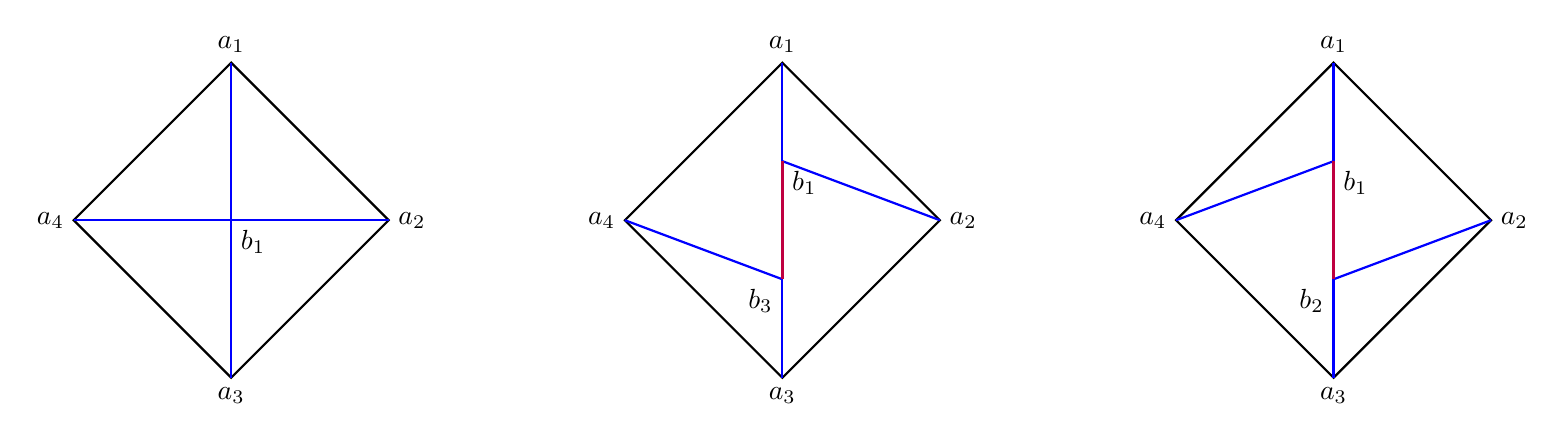
\begin{tikzpicture}
        % First Diagram
        % Define vertices
        \coordinate (A1) at (0, 2);
        \coordinate (A2) at (2, 0);
        \coordinate (A3) at (0, -2);
        \coordinate (A4) at (-2, 0);
        \coordinate (B1) at (0, 0);

        % Draw the diamond
        \draw[thick, black] (A1) -- (A2) -- (A3) -- (A4) -- cycle;

        % Draw blue lines
        \draw[thick, blue] (A1) -- (B1);
        \draw[thick, blue] (A2) -- (B1);
        \draw[thick, blue] (A3) -- (B1);
        \draw[thick, blue] (A4) -- (B1);

        % Label vertices
        \node[above] at (A1) {$a_1$};
        \node[right] at (A2) {$a_2$};
        \node[below] at (A3) {$a_3$};
        \node[left] at (A4) {$a_4$};
        \node[below right] at (B1) {$b_1$};

        % Second Diagram
        % Shifted to the right
        \begin{scope}[shift={(7, 0)}]
            % Define vertices
            \coordinate (A1) at (0, 2);
            \coordinate (A2) at (2, 0);
            \coordinate (A3) at (0, -2);
            \coordinate (A4) at (-2, 0);
            \coordinate (B1) at (0, 0.75);
            \coordinate (B2) at (0, -0.75);

            % Draw the diamond
            \draw[thick, black] (A1) -- (A2) -- (A3) -- (A4) -- cycle;

            % Draw blue lines
            \draw[thick, blue] (A1) -- (B1);
            \draw[thick, blue] (A2) -- (B1);
            \draw[thick, blue] (A3) -- (B2);
            \draw[thick, blue] (A4) -- (B2);

            % Draw the thick purple line
            \draw[very thick, purple] (B1) -- (B2);

            % Label vertices
            \node[above] at (A1) {$a_1$};
            \node[right] at (A2) {$a_2$};
            \node[below] at (A3) {$a_3$};
            \node[left] at (A4) {$a_4$};
            \node[below right] at (B1) {$b_1$};
            \node[below left] at (B2) {$b_3$};
        \end{scope}

        % Third Diagram
        % Shifted further to the right
         \begin{scope}[shift={(14, 0)}]
            % Define vertices
            \coordinate (A1) at (0, 2);
            \coordinate (A2) at (2, 0);
            \coordinate (A3) at (0, -2);
            \coordinate (A4) at (-2, 0);
            \coordinate (B1) at (0, 0.75);
            \coordinate (B2) at (0, -0.75);

            % Draw the diamond
            \draw[thick, black] (A1) -- (A2) -- (A3) -- (A4) -- cycle;

            % Draw blue lines
            \draw[thick, blue] (A1) -- (B1);
            \draw[thick, blue] (A4) -- (B1);
            \draw[thick, blue] (A3) -- (B2);
            \draw[thick, blue] (A2) -- (B2);

            % Draw the thick purple line
            \draw[very thick, purple] (B1) -- (B2);

            % Label vertices
            \node[above] at (A1) {$a_1$};
            \node[right] at (A2) {$a_2$};
            \node[below] at (A3) {$a_3$};
            \node[left] at (A4) {$a_4$};
            \node[below right] at (B1) {$b_1$};
            \node[below left] at (B2) {$b_2$};
        \end{scope}

    \end{tikzpicture}
    }
    \caption{Graphs for $n=4$}
    \label{fig_n=4}
\end{figure}
There are three graphs for the case $n = 4$, as in Figure \ref{fig_n=4}.  The blue edges are boundary edges and equal to $\Theta^{(B)}$. The purple edges are internal edges equal to  $\Theta^{(B)} - 1$.  The r.h.s. of \eqref{eq_trcalK} equals 

\begin{align}\nonumber
\sum_{\Gamma_{\textbf{a}}\, \in\,  {TSP}({\cal P}_{\textbf{a}})} \Gamma_{ \textbf{a}}(t, \boldsymbol{\sigma})= & \sum_{b_1, b_2, b_3, b_4}  \left(\prod_{i=1}^4 \left(\Theta^{(B)}_{t m_i m_{i+1}}\right)_{a_i b_i}\right) \times
\\\nonumber
& \times \left( \delta_{b_1 b_2 b_3 b_4}
+ \delta_{b_1 b_2} \delta_{b_3 b_4} \left(\Theta^{(B)}_{t m_1 m_3} - 1\right)_{b_1 b_3}
+ \delta_{b_1 b_4} \delta_{b_2 b_3} \left(\Theta^{(B)}_{t m_2 m_4} - 1\right)_{b_1 b_2}\right)
\end{align}

\begin{corollary}[Pure loop $\cal K$]\label{lem_pureloop} In the special case %$\sigma_k=1$ for $1\le k\le n$, i.e, 
$\sigma=(+,+\cdots +)$, we have 
\begin{align}\label{res_pureKes}\left|{\cal K}_{t, \boldsymbol{\sigma}, \textbf{a}}\right|\le C_n \exp\left(-c_n\max_{ij}\|a_i-a_j\|\right),\quad \|a_i-a_j\|:=\min_{q\in\mathbb Z}|a_i-a_j+qL|
\end{align} 
\end{corollary}
\begin{proof}[Proof of Corollary \ref{lem_pureloop}]
Since  $\sigma_i=+$ for all $i$,   $f_t(e)$ in \eqref{def_feRR} is either  $\Theta^{(B)}_{tm^2}$ or $\Theta^{(B)}_{tm^2}-1$. Applying  \eqref{prop:ThfadC} with $\xi=tm^2$, we obtain that $\|\Theta^{(B)}_{tm^2}\|_{\max}=O(1)$ and $\Theta^{(B)}_{tm^2}$ decays exponentially. Thus 
$$  \left|\Gamma^{(\textbf{b})}_{\textbf{a}}(t, \boldsymbol{\sigma})\right|\le C_n \exp\left(-c_n\max_{ij}\|b_i-b_j\|-c_n \max_{ij}\|a_i-b_j\|\right).
 $$
Together with the \eqref{def_Gatsiga} and \eqref{eq_trcalK}, we obtain the desired result \eqref{res_pureKes}. 
\end{proof}
\begin{proof}[Proof of Lemma \ref{Lemma_TRofK}]
 In this proof, we temporarily denote 
   $$
   \widetilde{ {\cal K}}_{t, \boldsymbol{\sigma}, \textbf{a}}:= m_{\boldsymbol{\sigma}}\cdot W^{-n+1}    \sum_{\Gamma_{\textbf{a}}\, \in\,  {TSP}({\cal P}_{\textbf{a}})}  \Gamma_{t, \boldsymbol{\sigma}, \textbf{a}},\quad \quad \quad \quad m_{\boldsymbol{\sigma}}:=\prod_{i=1}^n m(\sigma_i);
   $$
   We will show that 
  \begin{equation}\label{jlajus}
     \widetilde{ {\cal K}}_{t, \boldsymbol{\sigma}, \textbf{a}}
   =
    { {\cal K}}_{t, \boldsymbol{\sigma}, \textbf{a}},\quad  \text{for} \; \quad  t=0   \end{equation}
and   $\widetilde{\cal K}$ satisfies the dynamics equation for $ \cal K$ in \eqref{pro_dyncalK}, i.e., 
  \begin{align}\label{pjlacalK}
       \frac{d}{dt}\, \widetilde{ {\cal K}}_{t, \boldsymbol{\sigma}, \textbf{a}} 
       =  
       {W}\cdot  \sum_{1 \le k < l \le n} \sum_{a, b} \; \left( {\cal G}^{(a), L}_{k, l} \circ  \widetilde{ {\cal K}}_{t, \boldsymbol{\sigma}, \textbf{a}} \right) S^{(B)}_{ab} \left( {\cal G}^{(b), R}_{k, l} \circ  \widetilde{ {\cal K}}_{t, \boldsymbol{\sigma}, \textbf{a}} \right)  
    \end{align}
    here
    $$
    {\cal G}^{(a), L}_{k, l} \circ  \widetilde{ {\cal K}}_{t, \boldsymbol{\sigma}, \textbf{a}}  \,=\,\widetilde{ {\cal K}}_{t, \; {\cal G}^{(a), L}_{k, l}\left( \boldsymbol{\sigma}, \; \textbf{a}\right) } ,\quad \quad 
    \quad 
    {\cal G}^{(b), R}_{k, l} \circ  \widetilde{ {\cal K}}_{t, \boldsymbol{\sigma}, \textbf{a}} 
    \,=\,\widetilde{ {\cal K}}_{t, \; {\cal G}^{(b), R}_{k, l}\left( \boldsymbol{\sigma}, \; \textbf{a}\right) }.
    $$
    For  $t = 0$, we have  by definition that 
    $$
    t = 0 \implies \Theta^{(B)}_{t\, \xi} = I 
    $$
    If the tree graph $\Gamma$ has an internal edge,  then $\Gamma_{t, \boldsymbol{\sigma}, \textbf{a}} = 0$ when $t = 0$. Hence for $t=0$, the  only non-trivial graph is the star-shaped graph (Figure~\ref{fig_star}), which has only one internal vertex.
Hence  \eqref{jlajus} can be explicitly verified, i.e., 
$$
 \widetilde{{\cal K}}_{0, \boldsymbol{\sigma}, \textbf{a}} 
  =   m_{\boldsymbol{\sigma}} W^{ -n+1}\cdot\delta_{a_1, a_2, \dots, a_n}  
  = 
   W^{ -n+1}\Gamma^{(\text{star})}_{0, \boldsymbol{\sigma}, \textbf{a}} 
     = {\cal K}_{0, \boldsymbol{\sigma}, \textbf{a}} .
$$

\medskip
Now we prove \eqref{pjlacalK}. By definition,
$$
      \frac{d}{dt}\, \widetilde{ {\cal K}}_{t, \boldsymbol{\sigma}, \textbf{a}} =
     m_{\boldsymbol{\sigma}} W^{-n+1}\cdot \sum_{\Gamma_{\textbf{a}}\, \in\,  {TSP}({\cal P}_{\textbf{a}})} 
       \frac{d}{dt}\, \Gamma_{t, \boldsymbol{\sigma}
       , \textbf{a}}
       =   m_{\boldsymbol{\sigma}} W^{-n+1}\cdot \sum_{\Gamma_{\textbf{a}}\, \in\,  {TSP}({\cal P}_{\textbf{a}})}
       \sum_{\textbf{b}}
       \frac{d}{dt} \, \Gamma^{(\textbf{b})}_{t, \boldsymbol{\sigma}
       , \textbf{a}}
$$
 Recall $\Gamma^{(\textbf{b})}_{t, \boldsymbol{\sigma}, \textbf{a}}$ as defined in \eqref{defGabst}. 
 Due to $ d m_i/dt = 0$, the derivative $d/dt$  acts only on the $f_t(e)$.   By definition, 
       % of $\Gamma_{t, \boldsymbol{\sigma}, \textbf{a}}$ in \eqref{defGabst}. 
$$
\frac{d}{dt} \Theta^{(B)}_{t \xi} = \Theta^{(B)}_{t \xi} \cdot \xi S^{(B)} \cdot \Theta^{(B)}_{t \xi}
$$
Therefore, 
$$
\frac{d}{dt} \Theta^{(B)}_{t m_i m_j} = m_i m_j \left( \Theta^{(B)}_{t m_i m_j} \cdot S^{(B)} \cdot \Theta^{(B)}_{t m_i m_j}\right)
$$
In other words, the derivative of a blue edge $\Theta^{(B)}$ or a purple edge $\Theta^{(B)} - 1$ equals $m_i m_j$ times two blue edges with $S^{(B)}$ in the middle.

\begin{figure}[ht]
    \centering
    \begin{tikzpicture}[baseline=(current bounding box.center)]
        % First row: Blue derivative
        \node[blue] at (-2, 1) {\(\frac{d}{dt}\)};
        \draw[thick, blue] (-1.5, 1) -- (1.5, 1); % Blue horizontal line

        % Second row: Purple derivative
        \node[purple] at (-2, 0) {\(\frac{d}{dt}\)};
        \draw[thick, purple] (-1.5, 0) -- (1.5, 0); % Purple horizontal line

        % Equal sign
        \node at (2, 0.5) {\(=\)};

        % Right side: S^(b) and lines
        % Left blue line
        \draw[thick, blue] (2.5, 0.5) -- (4, 0.5);
        % Middle S^(b)
        \node at (4.5, 0.5) {\(S^{(B)}\)};
        % Right blue line
        \draw[thick, blue] (5 , 0.5) -- (6.5, 0.5);

        % Final blue line with "m j"
        
        \node at (7.5,0.5) {\( \cdot\; m_i m_j \)};
    \end{tikzpicture}
    \caption{Derivatives of edges}
\end{figure}


 On the other hand, we know that for fixed $\Gamma_\textbf{a}\in TSP({\cal P}_\textbf{a})$, $\boldsymbol{\sigma}$, $\textbf{a}$, $i$, $j$, there is at most one edge $e\in {\cal E}(\Gamma_\textbf{a})$ such that $e=R_i \cap R_j$. Then we can write the derivative of $\Gamma_{t, \boldsymbol{\sigma}, \textbf{a}}$  as follows
\begin{equation}\label{9aksufuo44}
  \frac{d}{dt} \, \Gamma^{(\textbf{b})}_{t, \,\boldsymbol{\sigma}
       ,\, \textbf{a}} = \sum_{1\le i < j\le n }\; \; \sum_{e\,\in \,{\cal E}(\Gamma_\textbf{a})} \textbf{1} \left(e=R_i\cap R_j\right) 
       \cdot \frac{\Gamma^{(\textbf{b})}_{t, \,\boldsymbol{\sigma}
       ,\, \textbf{a}}}{\left(f_t(e)\right)_{e_i,e_f}} 
       \cdot m_i \,m_j \,\left(\Theta^{(B)}_{t m_i m_j} \cdot S^{(B)} \cdot \Theta^{(B)}_{t m_i m_j}\right)_{e_i,e_f} 
\end{equation}
where $f_t(e)$ is defined in \eqref{def_feRR}. 
The quotient notation in \eqref{9aksufuo44} is symbolic and does not denote numerical division. Indeed, for \(e\in {\cal E}(\Gamma_\textbf{a})\) with \(e=R_i\cap R_j\), the definition
\eqref{defGabst} ensures that \((f_t(e))_{e_i,e_f}\) is one of the factors in
\(\Gamma^{(\textbf{b})}_{t,\boldsymbol{\sigma},\textbf{a}}\). Thus the quotient denotes the product defining \(\Gamma^{(\textbf{b})}_{t,\boldsymbol{\sigma},\textbf{a}}\) with this factor omitted.
 
Suppose  that there  exists $e\,\in \,{\cal E}(\Gamma_\textbf{a})$ such that  $e=R_i\cap R_j$.  Then 
$$
\frac{\Gamma^{(\textbf{b})}_{t, \,\boldsymbol{\sigma}
       ,\, \textbf{a}}}{\left(f_t(e)\right)_{e_i,e_f}} 
       \cdot m_i \,m_j \,\left(\Theta^{(B)}_{t m_i m_j} \cdot S^{(B)} \cdot \Theta^{(B)}_{t m_i m_j}\right)_{e_i,e_f}  ,\quad e=R_i\cap R_j 
       $$
    is equal to removing the edge $e$ in $\Gamma_\textbf{a}$ and adding two edges $\{e_i, a\}$, $\{e_f, b\}$, and a $S^{(B)}_{ab}$ in the middle. Here is an example with $i=1$ and $j=3$ in Figure \ref{fig:hexagons}. Note: this statement also holds for the case $|i-j|=1$. For example, if $i=1$, $j=2$, the triangle in the r.h.s. of Figure \ref{fig:hexagons} will become an $n=2$ polygon ${\cal P}_{(a_1,a)}$ with charge vector $(\sigma_1,\sigma_2)$ and a blue edge $(a_1,a)$ inside. 
   \begin{figure}[h!]
   \hspace{0.5in}
 \scalebox{0.8}{\begin{minipage}{0.55\textwidth}
   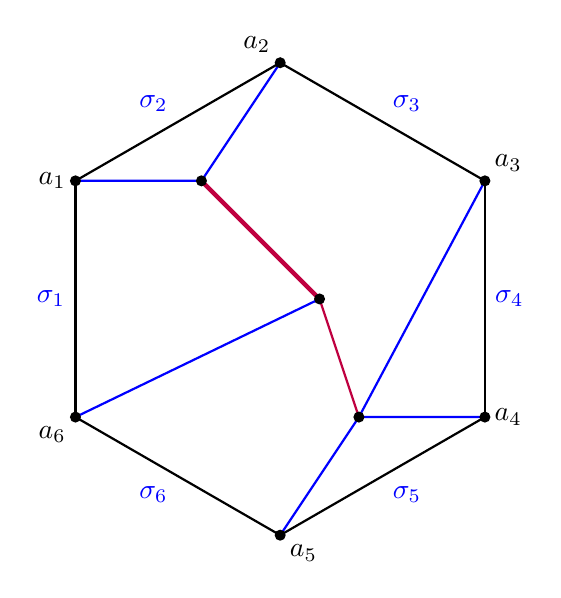
\begin{tikzpicture}
        % Define vertices of the hexagon
        \coordinate (A1) at (0, 3);      % Top
        \coordinate (A2) at (2.6, 1.5);  % Top-right
        \coordinate (A3) at (2.6, -1.5); % Bottom-right
        \coordinate (A4) at (0, -3);     % Bottom
        \coordinate (A5) at (-2.6, -1.5);% Bottom-left
        \coordinate (A6) at (-2.6, 1.5); % Top-left

        % Define inner intersection points
        \coordinate (B1) at (-1, 1.5);          % Near center but higher
        \coordinate (B2) at (-0.5, 1.0);        % Right-center
        \coordinate (B3) at (0, 0.5);       % Bottom-right center
        \coordinate (B4) at (0.5,  0);      % Bottom-left center
        \coordinate (B5) at (1, -1.5);       % Left-center

        % Draw hexagon outline with edge labels
        \draw[thick, black] (A1) -- (A2) node[midway, above right, blue] {$\sigma_3$};
        \draw[thick, black] (A2) -- (A3) node[midway, right, blue] {$\sigma_4$};
        \draw[thick, black] (A3) -- (A4) node[midway, below right, blue] {$\sigma_5$};
        \draw[thick, black] (A4) -- (A5) node[midway, below left, blue] {$\sigma_6$};
        \draw[thick, black] (A5) -- (A6) node[midway, left, blue] {$\sigma_1$};
        \draw[thick, black] (A6) -- (A1) node[midway, above left, blue] {$\sigma_2$};

        % Draw red lines from vertices to the intermediate points
       \draw[thick, blue] (A1) -- (B1) -- (A6);
        \draw[ultra thick, purple] (B1) -- (B4); 
        \draw[thick, blue] (B4) -- (A5);
        \draw[thick, purple] (B4) -- (B5) ;
        \draw[thick, blue] (B5) -- (A2);
        \draw[thick, blue] (A3) -- (B5) -- (A4);

        % Draw dashed lines from vertices to the opposite inner points
       % \draw[thick, black, dashed] (A1) -- (B2)--(A6);
       % \draw[thick, black, dashed] (A2) -- (B3)--(A5);

        % Draw dots at vertices and inner points
        \fill[black] (A1) circle (2pt);
        \fill[black] (A2) circle (2pt);
        \fill[black] (A3) circle (2pt);
        \fill[black] (A4) circle (2pt);
        \fill[black] (A5) circle (2pt);
        \fill[black] (A6) circle (2pt);
        \fill[black] (B1) circle (2pt);
        %\fill[black] (B2) circle (2pt);
       % \fill[black] (B3) circle (2pt);
        \fill[black] (B4) circle (2pt);
        \fill[black] (B5) circle (2pt);
        
        % Label outer vertices
        \node[above left] at (A1) {$a_2$};
        \node[above right] at (A2) {$a_3$};
        \node[right] at (A3) {$a_4$};
        \node[below right] at (A4) {$a_5$};
        \node[below left] at (A5) {$a_6$};
        \node[left] at (A6) {$a_1$};
        
    \end{tikzpicture}
\end{minipage}
\hfill
\begin{minipage}{0.45\textwidth}
    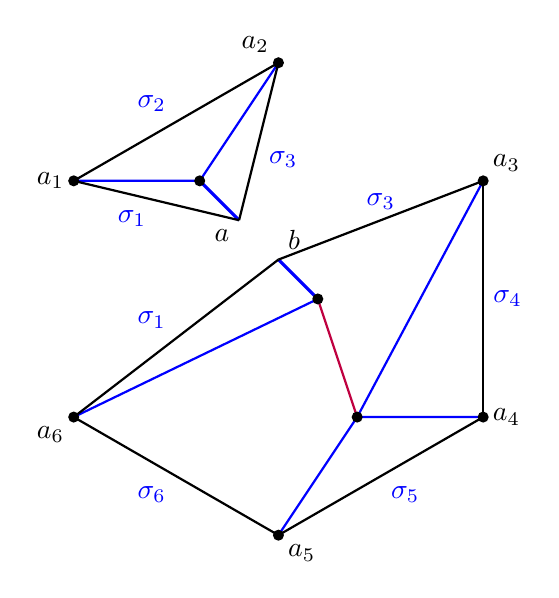
\begin{tikzpicture}
     
        % Define vertices of the hexagon
        \coordinate (A1) at (0, 3);      % Top
        \coordinate (A2) at (2.6, 1.5);  % Top-right
        \coordinate (A3) at (2.6, -1.5); % Bottom-right
        \coordinate (A4) at (0, -3);     % Bottom
        \coordinate (A5) at (-2.6, -1.5);% Bottom-left
        \coordinate (A6) at (-2.6, 1.5); % Top-left

        % Define inner intersection points
        \coordinate (B1) at (-1, 1.5);          % Near center but higher
        \coordinate (B2) at (-0.5, 1.0);        % Right-center
        \coordinate (B3) at (0, 0.5);       % Bottom-right center
        \coordinate (B4) at (0.5,  0);      % Bottom-left center
        \coordinate (B5) at (1, -1.5);       % Left-center

        % Draw hexagon outline with edge labels
        %\draw[thick, blue] (A1) -- (A2) node[midway, above right, blue] {$e_3$};
        \draw[thick, black] (A2) -- (A3) node[midway, right, blue] {$\sigma_4$};
        \draw[thick, black] (A3) -- (A4) node[midway, below right, blue] {$\sigma_5$};
        \draw[thick, black] (A4) -- (A5) node[midway, below left, blue] {$\sigma_6$};
       % \draw[thick, blue] (A5) -- (A6) node[midway, left, blue] {$e_1$};
        \draw[thick, black] (A6) -- (A1) node[midway, above left, blue] {$\sigma_2$};

        % Draw red lines from vertices to the intermediate points
        \draw[thick, blue] (A1) -- (B1) -- (A6);
        \draw[ very thick, blue] (B1) -- (B2); 
        \draw[ very thick, blue] (B3) -- (B4); 
        \draw[thick, blue] (B4) -- (A5);
        \draw[thick, purple] (B4) -- (B5) ;
        \draw[thick, blue] (B5) -- (A2);
        \draw[thick, blue] (A3) -- (B5) -- (A4);

        % Draw dashed lines from vertices to the opposite inner points
        \draw[thick, black ] (A1) -- (B2) 
        node[midway, below right, blue]{$\sigma_3$};
         \draw[thick, black ] (B2)--(A6)
         node[midway, below left, blue]{$\sigma_1$};
        \draw[thick, black ] (A2) -- (B3) 
        node[midway, above  , blue]{$\sigma_3$};
         \draw[thick, black ] (B3)--(A5)
         node[midway, above left , blue]{$\sigma_1$};

        % Draw dots at vertices and inner points
        \fill[black] (A1) circle (2pt);
        \fill[black] (A2) circle (2pt);
        \fill[black] (A3) circle (2pt);
        \fill[black] (A4) circle (2pt);
        \fill[black] (A5) circle (2pt);
        \fill[black] (A6) circle (2pt);
        \fill[black] (B1) circle (2pt);
        %\fill[black] (B2) circle (2pt);
       % \fill[black] (B3) circle (2pt);
        \fill[black] (B4) circle (2pt);
        \fill[black] (B5) circle (2pt);

       % Label outer vertices
        \node[above left] at (A1) {$a_2$};
        \node[above right] at (A2) {$a_3$};
        \node[right] at (A3) {$a_4$};
        \node[below right] at (A4) {$a_5$};
        \node[below left] at (A5) {$a_6$};
        \node[left] at (A6) {$a_1$};
 \node[below left] at (B2) {$a $}; 
 \node[above right] at (B3) {$b $};
 
 \end{tikzpicture}
  

   \end{minipage}
 
}
  \caption{Derivative of tree}
    \label{fig:hexagons}
\end{figure}

 
 
The new edges created by the partition will inherit the original charges. We denote them by 
\begin{equation}
\label{zzzrelation}
(\boldsymbol{\sigma}', \textbf{a}')= {\cal G}^{(a), L}_{i, j}(\boldsymbol{\sigma}, \textbf{a}) \quad\quad 
(\boldsymbol{\sigma}'', \textbf{a}'')={\cal G}^{(b), R}_{i, j}(\boldsymbol{\sigma}, \textbf{a}).
\end{equation}
%If $e=R_i\cap R_j$, then by definition, it is easy to see that 
Therefore, there exist 
$\Gamma'_{\textbf{a}'}\in TSP({\cal P}_{\textbf{a}'})$ and $ \Gamma''_{\textbf{a}''}\in TSP({\cal P}_{\textbf{a}''})$  such that (as in Figure \ref{fig:hexagons})
$$
  m_{\boldsymbol{\sigma}}\cdot \sum_{\textbf{b}}\frac{\Gamma^{(\textbf{b})}_{t, \,\boldsymbol{\sigma}
       ,\, \textbf{a}}}{\left(f_t(e)\right)_{e_i,e_f}} 
       \cdot m_i \,m_j \,\left(\Theta^{(B)}_{t m_i m_j} \cdot S^{(B)} \cdot \Theta^{(B)}_{t m_i m_j}\right)_{e_i,e_f}     = \sum_{a, b} 
        m_{\boldsymbol{\sigma}'}\cdot \Gamma'_{t, \boldsymbol{\sigma}', \textbf{a}'} \cdot S^{(B)}_{ab} \cdot 
         m_{\boldsymbol{\sigma}''}\Gamma''_{t, \boldsymbol{\sigma}'', \textbf{a}''}.
$$
Thus,
$$
 m_{\boldsymbol{\sigma}}\cdot \frac{d}{dt} \sum_{\Gamma} \Gamma_{t, \boldsymbol{\sigma}, \textbf{a}} = \sum_{i < j} \sum_{a, b} \left(m_{\boldsymbol{\sigma}'}\sum_{\Gamma'} \Gamma'_{t, \boldsymbol{\sigma}', \textbf{a}'}\right) \cdot S^{(B)}_{ab} \cdot \left(m_{\boldsymbol{\sigma}''}\sum_{\Gamma''} \Gamma''_{t, \boldsymbol{\sigma}'', \textbf{a}''}\right)
$$
where $i$, $j$, $a$, $b$, $\boldsymbol{\sigma}$, $\textbf{a}$, $\boldsymbol{\sigma}'$, $\textbf{a}'$, $\boldsymbol{\sigma}''$, and $\textbf{a}''$ satisfy relation \eqref{zzzrelation}. Clearly it is equivalent to \eqref{pjlacalK} and this completes the proof of Lemma  \ref{Lemma_TRofK}.  

 \end{proof}



\subsection{Ward's identity on \texorpdfstring{$\cal K$}{K}}
Recall Ward's identity for resolvents, which states that
$$
G \cdot G^\dagger =G(z)\cdot G^\dagger(z)=G(z)\cdot G(\bar z)=\frac{G(z)-G(\bar z)}{z-\bar z}= \frac{G-G^\dagger}{2i\eta}, \quad \eta=\im z.
$$
In our setting, $G_t(+)=(H_t-z_t)^{-1}=\left(G_t(-)\right)^\dagger $ and thus
\begin{equation}
    \label{WI_2G}
G_t(+)\cdot G_t(-)= \frac{G_t(+)-G_t(-)}{2i\eta_t}=\frac{G_t(+)-G_t(-)}{ 2i (1-t)\im m},\quad \eta_t=\im z_t.
\end{equation}
 From Ward's identity, we  have the following identity for a $2$-$G$-loop: 
$$
\sum_a {\cal L}_{t, (+,-), (a,b)}=\frac{1}{2Wi\eta_t}\left({\cal L}_{t, (+), (b)}-{\cal L}_{t, (-), (b)}\right).
$$
We extend this identity  to all $n-G$ loops ${\cal L}$  in the following lemma. The main purpose of this subsection is to show that the same identity holds for  $\cal K$
loop as well. 

\begin{lemma}\label{lem_WI_K} For an $n$-$G$-loop ${\cal L}_{t, \boldsymbol{\sigma}, \textbf{a}}$ with 
$\sigma_1=+$ and $\sigma_n=-$, 
we have
\begin{equation}\label{WI_calL}
  \sum_{a_n}{\cal L}_{t, \boldsymbol{\sigma}, \textbf{a}}=
\frac{1}{2Wi\eta_t}\left({\cal L}_{t, \; \boldsymbol{\sigma}+,  \; \textbf{a}/a_n}- {\cal L}_{t, \; \boldsymbol{\sigma}-,  \; \textbf{a}/a_n}\right)  
\end{equation}
and
\begin{equation}\label{WI_calK}
  \sum_{a_n}{\cal K}_{t, \boldsymbol{\sigma}, \textbf{a}}=
\frac{1}{2Wi\eta_t}\left({\cal K}_{t, \; \boldsymbol{\sigma}+,  \; \textbf{a}/a_n}
- {\cal K}_{t, \; \boldsymbol{\sigma}-,  \; \textbf{a}/a_n}\right)  
\end{equation}
where 
\begin{itemize}
\item  $\boldsymbol{\sigma}\pm$ is obtained by removing $\sigma_n$ from $\boldsymbol{\sigma}$ and replacing $\sigma_1$ with $\pm$, i.e., 
    $$
\boldsymbol{\sigma}\pm=(\pm, \sigma_2, \sigma_3,\cdots \sigma_{ n-1}).$$
Notice that  the length of $\boldsymbol{\sigma}\pm$ is $n-1$. 
\item  $\textbf{a}/a_n$ is obtained by removing $a_n$ from $\textbf{a}$:
 $$
\textbf{a}/a_n=(a_1, a_2,a_3,\cdots, a_{n-1})
$$
\end{itemize}
\end{lemma}

\begin{corollary}\label{lem_sumAinK}
    Under the assumption of Lemma \ref{lem_WI_K}, we have 
\begin{align}\label{sumallAinK}
      \sum_{a_2}\cdots\sum_{a_{n-1}}\sum_{a_n}{\cal K}_{t, \boldsymbol{\sigma}, \textbf{a}}=O((W\eta_t)^{-n+1})
\end{align}
 \end{corollary}
 


\begin{proof}[Proof of Corollary \ref{lem_sumAinK}]
By definition of $\cal K$, we know that ${\cal K}$ is  translation invariant. Then the left side  of equation \eqref{sumallAinK} is independent of $a_1$. 
Hence it is equivalent to 
$$
 \frac1L\sum_{\textbf{a}\in\mathbb Z_L^n}{\cal K}_{t, \boldsymbol{\sigma}, \textbf{a}}=O((W\eta_t)^{-n+1}).
$$
 Applying \eqref{WI_calK} repeatedly, we can reduce it to shorter pure loops to get  
\begin{align}\label{sfauuu}
 \Big | L^{-1}\cdot \sum_{\textbf{a}\in\mathbb Z_L^n}{\cal K}_{t, \boldsymbol{\sigma}, \textbf{a}}\Big |
  \le C_n \sum_{1\le m\le n}(W\eta_t)^{-n+m}\cdot L^{-1}\cdot
  \max_{\boldsymbol{\sigma}'\in \{+\}^m \cup \{-\}^m}\left| \sum_{\textbf{a}'\in\mathbb Z_L^m}{\cal K}_{t, \boldsymbol{\sigma}', \textbf{a}'}\right|,\quad 
\end{align}
Here $\boldsymbol{\sigma}'\in \{+\}^m \cup \{-\}^m$ means that $\boldsymbol{\sigma}'=(+,+,\cdots,+)\; \hbox{or }(-,-,\cdots,-)$.
By the estimate of pure loop $\cal K$  in   Lemma \ref{lem_pureloop}, we have 
$$
\sum_{\textbf{a}'\in\mathbb Z_L^m}{\cal K}_{t, \boldsymbol{\sigma}', \textbf{a}'}=O(1).
$$
Together with \eqref{sfauuu}, this  completes the proof of the corollary. 

\end{proof}



\bigskip

 \begin{proof}[Proof of Lemma \ref{lem_WI_K}]
We divide the proof into five steps. The main idea is to show that the
difference between the two sides of \eqref{WI_calK} satisfies a homogeneous
linear differential equation with zero initial value.

\medskip
\noindent{\textbf{Step 1: The identity for ${\cal L}$ and the cases $n=2,3$ for $\cal K$.}}

Since $\sum_{a_n}E_{a_n}=W^{-1}I$, cyclicity of the trace and the
two-resolvent Ward identity give
\begin{align*}
 \sum_{a_n}{\cal L}_{t,\boldsymbol{\sigma},\textbf{a}}
 &=
 \frac1W
 \left\langle
 G_t(-)G_t(+)
 E_{a_1}\prod_{j=2}^{n-1}G_t(\sigma_j)E_{a_j}
 \right\rangle                                                \\
 &=
 \frac{1}{2Wi\eta_t}
 \left(
 {\cal L}_{t,\boldsymbol{\sigma}+,\textbf{a}/a_n}
 -{\cal L}_{t,\boldsymbol{\sigma}-,\textbf{a}/a_n}
 \right).
\end{align*}
This proves \eqref{WI_calL}.

We next prove \eqref{WI_calK}. For $n=2$, the explicit two-loop formula and
the stochasticity of $S^{(B)}$ yield
\begin{equation}\label{hsgw2}
 \sum_{a_2}{\cal K}_{t,(+,-),(a_1,a_2)}
 =
 \frac1W\sum_{a_2}
 \left(\frac{|m|^2}{1-t|m|^2S^{(B)}}\right)_{a_1a_2}
 =\frac{1}{W(1-t)}.
\end{equation}
On the other hand,
\[
 \frac{{\cal K}_{t,+,a_1}-{\cal K}_{t,-,a_1}}{2Wi\eta_t}
 =\frac{m-\bar m}{2Wi\eta_t}
 =\frac{1}{W(1-t)},
\]
where we used $|m|=1$, $m-\bar m=2i\im m$, and
$\eta_t=(1-t)\im m$.

For completeness, we give the calculation for $n=3$. This also provides
a representative example of the algebra used below. Put
\[
 q:=m(\sigma_2),\qquad
 A:=\Theta^{(B)}_{tmq},\qquad
 B:=\Theta^{(B)}_{t\bar m q}.
\]
Since $\sigma_1=+$ and $\sigma_3=-$, the explicit three-loop formula gives
\[
 \sum_{a_3}{\cal K}_{t,(+,\sigma_2,-),(a_1,a_2,a_3)}
 =\frac{q}{W^2(1-t)}(AB)_{a_1a_2}.
\]
Here we used
\[
 \sum_{a_3}(\Theta^{(B)}_t)_{a_3x}=\frac{1}{1-t}
\]
and the fact that all propagators are functions of $S^{(B)}$ and hence
commute. The two loops on the right-hand side of \eqref{WI_calK} are
\[
 {\cal K}_{t,(+,\sigma_2),(a_1,a_2)}=\frac{mq}{W}A_{a_1a_2},
 \qquad
 {\cal K}_{t,(-,\sigma_2),(a_1,a_2)}=\frac{\bar m q}{W}B_{a_1a_2}.
\]
The required matrix identity follows directly from the definitions of
$A$ and $B$:
\begin{align*}
 mA-\bar mB
 &=AB\bigl(mB^{-1}-\bar mA^{-1}\bigr)                         \\
 &=AB\left[
 m\bigl(1-t\bar m qS^{(B)}\bigr)
 -\bar m\bigl(1-tmqS^{(B)}\bigr)
 \right]                                                       \\
 &=(m-\bar m)AB.
\end{align*}

\noindent Consequently,
\[
 \frac{
 {\cal K}_{t,(+,\sigma_2),(a_1,a_2)}
 -{\cal K}_{t,(-,\sigma_2),(a_1,a_2)}
 }{2Wi\eta_t}
 =\frac{q}{W^2(1-t)}(AB)_{a_1a_2},
\]
which proves \eqref{WI_calK} for $n=3$.

\medskip
\noindent{\textbf{Step 2: Induction and the difference equation.}}

Let $n\geq4$ and assume that \eqref{WI_calK} holds for all loops of length
strictly smaller than $n$. Define
\begin{equation}\label{def_calKpm}
 {\cal K}^{(*)}_{t,\boldsymbol{\sigma},\textbf{a}}
 :=\sum_{a_n}{\cal K}_{t,\boldsymbol{\sigma},\textbf{a}},
 \qquad
 {\cal K}^{(\pm)}_{t,\boldsymbol{\sigma},\textbf{a}}
 :={\cal K}_{t,\boldsymbol{\sigma}\pm,\textbf{a}/a_n},
\end{equation}
and
\[
 {\cal K}^{(**)}_{t,\boldsymbol{\sigma},\textbf{a}}
 :=\frac{{\cal K}^{(+)}_{t,\boldsymbol{\sigma},\textbf{a}}
 -{\cal K}^{(-)}_{t,\boldsymbol{\sigma},\textbf{a}}}{2Wi\eta_t},
 \qquad
 D_{t,\boldsymbol{\sigma},\textbf{a}}:={\cal K}^{(*)}_{t,\boldsymbol{\sigma},\textbf{a}}
 -{\cal K}^{(**)}_{t,\boldsymbol{\sigma},\textbf{a}}.
\]
We shall prove that $D$ vanishes identically. More precisely, the induction
will be closed once we establish
\begin{equation}\label{finK*-K}
\begin{aligned}
 \partial_tD_{t,\boldsymbol{\sigma},\textbf{a}}
 &=W\sum_{k=1}^{n-1}\sum_{a,b}
 D_{t,\boldsymbol{\sigma},\textbf{a}}\big|_{a_k\to a}
 S^{(B)}_{ab}{\cal K}_{t,(\sigma_k,\sigma_{k+1}),(a_k,b)}\\
 &\quad+\frac{1}{1-t}D_{t,\boldsymbol{\sigma},\textbf{a}}.
\end{aligned}
\end{equation}

At $t=0$, the initial condition for the primitive equation gives
\begin{align*}
 {\cal K}^{(*)}_{0,\boldsymbol{\sigma},\textbf{a}}
 &=W^{-n+1}
 \left(\prod_{j=2}^{n-1}m(\sigma_j)\right)
 \mathbf 1(a_1=\cdots=a_{n-1}),                                    \\
 {\cal K}^{(**)}_{0,\boldsymbol{\sigma},\textbf{a}}
 &=\frac{W^{-n+2}(m-\bar m)}{2Wi\eta_0}
 \left(\prod_{j=2}^{n-1}m(\sigma_j)\right)
 \mathbf 1(a_1=\cdots=a_{n-1}).
\end{align*}
Since $\eta_0=\im m$, these expressions are equal. Thus $D_0=0$.

For $1\leq k<l\leq n$, abbreviate
\[
 \mathcal J^L_{k,l,a}:={\cal G}^{(a),L}_{k,l}\circ
 {\cal K}_{t,\boldsymbol{\sigma},\textbf{a}},
 \qquad
 \mathcal J^R_{k,l,b}:={\cal G}^{(b),R}_{k,l}\circ
 {\cal K}_{t,\boldsymbol{\sigma},\textbf{a}},
\]
and define $\mathcal J^{L,(\pm)}$ and $\mathcal J^{R,(\pm)}$ analogously
with ${\cal K}^{(\pm)}$ in place of ${\cal K}$. The primitive equation gives
\begin{equation}\label{gsasawwe}
 \partial_t{\cal K}^{(*)}
 =W\sum_{1\leq k<l\leq n}\sum_{a,b}
 \left(\sum_{a_n}\mathcal J^L_{k,l,a}\right)
 S^{(B)}_{ab}\mathcal J^R_{k,l,b}.
\end{equation}
Moreover, since $\partial_t\eta_t^{-1}=(1-t)^{-1}\eta_t^{-1}$,
\begin{equation}\label{gsasawII}
\begin{aligned}
 \partial_t{\cal K}^{(**)}
 &=\frac{1}{1-t}{\cal K}^{(**)}                                  \\
 &\quad+\frac{W}{2Wi\eta_t}
 \sum_{1\leq k<l\leq n-1}\sum_{a,b}
 \left(
 \mathcal J^{L,(+)}_{k,l,a}\mathcal J^{R,(+)}_{k,l,b}
 -\mathcal J^{L,(-)}_{k,l,a}\mathcal J^{R,(-)}_{k,l,b}
 \right)S^{(B)}_{ab}.
\end{aligned}
\end{equation}

\medskip
\noindent{\textit{Road map for Steps 3--4.}}
To compare these two derivatives, we partition the pairs $(k,l)$ into
four classes. The following are the four claims that will be verified
below.
\begin{enumerate}
 \item For $2\leq k<l\leq n-1$, the non-adjacent terms $l\geq k+2$
 cancel by the induction hypothesis, while the adjacent terms give
 \[
  W\sum_{k=2}^{n-2}\sum_{a,b}
  D_{t,\boldsymbol{\sigma},\textbf{a}}\big|_{a_k\to a}
  S^{(B)}_{ab}{\cal K}_{t,(\sigma_k,\sigma_{k+1}),(a_k,b)}.
 \]

 \item For each $3\leq m\leq n-2$, the two boundary cuts $(1,m)$ and
 $(m,n)$ cancel after applying the induction hypothesis and using the
 symmetry of $S^{(B)}$.

 \item The cut $(1,n)$ contributes $(1-t)^{-1}{\cal K}^{(*)}$. Together
 with the derivative of $\eta_t^{-1}$ in $\partial_t{\cal K}^{(**)}$, this
 produces $(1-t)^{-1}D$.

 \item The four remaining cuts
 $(1,2)$, $(1,n-1)$, $(2,n)$ and $(n-1,n)$ 
 give the two endpoint terms
 \[
  W\sum_{k\in\{1,n-1\}}\sum_{a,b}
  D_{t,\boldsymbol{\sigma},\textbf{a}}\big|_{a_k\to a}
  S^{(B)}_{ab}{\cal K}_{t,(\sigma_k,\sigma_{k+1}),(a_k,b)}.
 \]
\end{enumerate}
Step 3 proves the first claim, and Step 4 proves the remaining three.

\medskip
\noindent{\textbf{Step 3: Internal cuts.}}

Suppose that $2\leq k<l\leq n-1$. The right loop produced by the
cut-and-glue operation is explicitly
\[
 \mathcal J^R_{k,l,b}
 ={\cal K}_{t,(\sigma_k,\ldots,\sigma_l),
 (a_k,\ldots,a_{l-1},b)}.
\]
Changing the first charge of the original loop or removing its last charge
does not affect this segment. Hence
\begin{equation}\label{kdjuwsz}
 \mathcal J^{R,(+)}_{k,l,b}
 =\mathcal J^{R,(-)}_{k,l,b}
 =\mathcal J^R_{k,l,b}.
\end{equation}
This is a representative calculation behind the corresponding
cut-and-glue identities used in the proof.

If $l\geq k+2$, the left loop has length at most $n-1$. The induction
hypothesis therefore gives
\begin{equation}\label{a';slw}
 \sum_{a_n}\mathcal J^L_{k,l,a}
 =\frac{\mathcal J^{L,(+)}_{k,l,a}
 -\mathcal J^{L,(-)}_{k,l,a}}{2Wi\eta_t}.
\end{equation}
Thus all non-adjacent internal cuts cancel between
$\partial_t{\cal K}^{(*)}$ and $\partial_t{\cal K}^{(**)}$.

If $l=k+1$, then
\begin{equation}\label{uaiw03}
\begin{aligned}
 \mathcal J^L_{k,k+1,a}
 ={\cal K}_{t,\boldsymbol{\sigma},\textbf{a}}\big|_{a_k\to a},
 \qquad
 \mathcal J^R_{k,k+1,b}
 ={\cal K}_{t,(\sigma_k,\sigma_{k+1}),(a_k,b)}.
\end{aligned}
\end{equation}
Therefore, the contribution of all adjacent internal cuts is
\begin{equation}\label{WI-pr-Mid}
 W\sum_{k=2}^{n-2}\sum_{a,b}
 D_{t,\boldsymbol{\sigma},\textbf{a}}\big|_{a_k\to a}
 S^{(B)}_{ab}{\cal K}_{t,(\sigma_k,\sigma_{k+1}),(a_k,b)}.
\end{equation}

\medskip
\noindent{\textbf{Step 4: Boundary cuts.}}

We first consider $(k,l)=(1,n)$. In this case
\[
 \mathcal J^L_{1,n,a}={\cal K}_{t,(+,-),(a,a_n)},
 \qquad
 \mathcal J^R_{1,n,b}
 ={\cal K}_{t,\boldsymbol{\sigma},\textbf{a}}\big|_{a_n\to b}.
\]
Using the already proved two-loop identity and
$\sum_aS^{(B)}_{ab}=1$, we obtain
\begin{equation}\label{nssfku}
 W\sum_{a,b,a_n}
 \mathcal J^L_{1,n,a}S^{(B)}_{ab}\mathcal J^R_{1,n,b}
 =\frac{1}{1-t}{\cal K}^{(*)}_{t,\boldsymbol{\sigma},\textbf{a}}.
\end{equation}

Next fix $3\leq m\leq n-2$. The two boundary cuts under consideration are
\begin{equation}\label{consjahz}
 (k,l)=(1,m)\quad\text{and}\quad(k,l)=(m,n),
 \qquad 3\leq m\leq n-2.
\end{equation}
Denote their respective contributions to $\partial_tD$ by $C_{1,m}$ and
$C_{m,n}$. Applying the induction hypothesis to the shorter left loop shows
that
\begin{equation}\label{awslw22}
 C_{1,m}=\frac{W}{2Wi\eta_t}\sum_{a,b}
 \mathcal J^{L,(-)}_{1,m,a}
 \left(\mathcal J^{R,(-)}_{1,m,b}
 -\mathcal J^{R,(+)}_{1,m,b}\right)S^{(B)}_{ab}.
\end{equation}
After interchanging $a$ and $b$, the cut $(m,n)$ gives
\begin{equation}\label{awslw33}
 C_{m,n}=-\frac{W}{2Wi\eta_t}\sum_{a,b}
 \mathcal J^{L,(-)}_{1,m,a}
 \left(\mathcal J^{R,(-)}_{1,m,b}
 -\mathcal J^{R,(+)}_{1,m,b}\right)S^{(B)}_{ab}.
\end{equation}
Here we used the symmetry of $S^{(B)}$. Hence
\begin{equation}\label{uisiip}
 C_{1,m}+C_{m,n}=0.
\end{equation}

It remains to consider
\begin{equation}\label{keayew}
 (1,2),\qquad (1,n-1),\qquad (2,n),\qquad (n-1,n).
\end{equation}
To keep track of the four terms, introduce the notation
\begin{equation}
 U_a^\pm:=\mathcal J^{L,(\pm)}_{1,2,a},
 \quad u_b^\pm:=\mathcal J^{R,(\pm)}_{1,2,b},
 \quad v_a^\pm:=\mathcal J^{L,(\pm)}_{1,n-1,a},
 \quad V_b^\pm:=\mathcal J^{R,(\pm)}_{1,n-1,b}.
\end{equation}
Thus $U^\pm,V^\pm$ are loops of length $n-1$, whereas $u^\pm,v^\pm$
are two-loops. In particular,
\begin{equation}
 {\cal K}^{(**)}\big|_{a_1\to a}
 =\frac{U_a^+-U_a^-}{2Wi\eta_t},
 \qquad
 {\cal K}^{(**)}\big|_{a_{n-1}\to a}
 =\frac{V_a^+-V_a^-}{2Wi\eta_t}.
\end{equation}

We now list the four full-loop contributions explicitly. For the two
adjacent cuts, the left loop is the original loop with one index replaced:
\begin{align*}
 \sum_{a_n}\mathcal J^L_{1,2,a}
 &={\cal K}^{(*)}\big|_{a_1\to a},
 &\mathcal J^R_{1,2,b}&=u_b^+,\\
 \sum_{a_n}\mathcal J^L_{n-1,n,a}
 &={\cal K}^{(*)}\big|_{a_{n-1}\to a},
 &\mathcal J^R_{n-1,n,b}&=v_b^-.
\end{align*}
In the second identity we used cyclicity to identify
$v_b^-={\cal K}_{t,(\sigma_{n-1},-),(a_{n-1},b)}$.

For the remaining cuts $(1,n-1)$ and $(2,n)$, the left loops have length
three. Applying the three-loop Ward identity from Step 1 gives
\begin{equation}
\begin{aligned}
 \sum_{a_n}\mathcal J^L_{1,n-1,a}
 &=\frac{v_a^+-v_a^-}{2Wi\eta_t},
 &\mathcal J^R_{1,n-1,b}&=V_b^+,\\
 \sum_{a_n}\mathcal J^L_{2,n,a}
 &=\frac{u_a^+-u_a^-}{2Wi\eta_t},
 &\mathcal J^R_{2,n,b}&=U_b^-.
\end{aligned}
\end{equation}
For example, the second line follows from
\begin{align*}
 \sum_{a_n}
 {\cal K}_{t,(+,\sigma_2,-),(a_1,a,a_n)}
 &=\frac{1}{2Wi\eta_t}
 \left[
 {\cal K}_{t,(+,\sigma_2),(a_1,a)}
 -{\cal K}_{t,(\sigma_2,-),(a,a_1)}
 \right] =\frac{u_a^+-u_a^-}{2Wi\eta_t},
\end{align*}
where the last equality again uses cyclicity of the two-loop.

We next compare these four terms with the $(1,2)$ and $(1,n-1)$ terms
in $\partial_t{\cal K}^{(**)}$. The latter are
\begin{align*}
 \frac{W}{2Wi\eta_t}\sum_{a,b}
 \bigl(
 U_a^+u_b^+-U_a^-u_b^-
 +v_a^+V_b^+-v_a^-V_b^-
 \bigr)S^{(B)}_{ab}.
\end{align*}
For the left endpoint, the cuts $(1,2)$ and $(2,n)$, after subtracting
the $(1,2)$ term above, give
\begin{align*}
 &W\sum_{a,b}{\cal K}^{(*)}\big|_{a_1\to a}S^{(B)}_{ab}u_b^+
 +\frac{W}{2Wi\eta_t}\sum_{a,b}
 (u_a^+-u_a^-)S^{(B)}_{ab}U_b^- 
 -\frac{W}{2Wi\eta_t}\sum_{a,b}
 (U_a^+u_b^+-U_a^-u_b^-)S^{(B)}_{ab}\\
 =&\;W\sum_{a,b}
 \left({\cal K}^{(*)}\big|_{a_1\to a}
 -\frac{U_a^+-U_a^-}{2Wi\eta_t}\right)
 S^{(B)}_{ab}u_b^+\\
 =&\;W\sum_{a,b}D\big|_{a_1\to a}S^{(B)}_{ab}
 {\cal K}_{t,(\sigma_1,\sigma_2),(a_1,b)}.
\end{align*}
Here the symmetry of $S^{(B)}$ was used in the first equality to interchange
$a$ and $b$ in the middle term.

Similarly, the cuts $(1,n-1)$ and $(n-1,n)$, after subtracting the
$(1,n-1)$ term in $\partial_t{\cal K}^{(**)}$, give
\begin{align*}
 &W\sum_{a,b}{\cal K}^{(*)}\big|_{a_{n-1}\to a}S^{(B)}_{ab}v_b^-
 +\frac{W}{2Wi\eta_t}\sum_{a,b}
 (v_a^+-v_a^-)S^{(B)}_{ab}V_b^+ 
 -\frac{W}{2Wi\eta_t}\sum_{a,b}
 (v_a^+V_b^+-v_a^-V_b^-)S^{(B)}_{ab}\\
=&\;W\sum_{a,b}
 \left({\cal K}^{(*)}\big|_{a_{n-1}\to a}
 -\frac{V_a^+-V_a^-}{2Wi\eta_t}\right)
 S^{(B)}_{ab}v_b^-\\
=&\;W\sum_{a,b}D\big|_{a_{n-1}\to a}S^{(B)}_{ab}
 {\cal K}_{t,(\sigma_{n-1},\sigma_n),(a_{n-1},b)}.
\end{align*}
Therefore the total contribution of the four remaining cuts is
\begin{equation}\label{uisiip222}
 W\sum_{k\in\{1,n-1\}}\sum_{a,b}
 D_{t,\boldsymbol{\sigma},\textbf{a}}\big|_{a_k\to a}
 S^{(B)}_{ab}{\cal K}_{t,(\sigma_k,\sigma_{k+1}),(a_k,b)}.
\end{equation}

\medskip
\noindent{\textbf{Step 5: Closing the induction.}}

Combining Steps 2--4, we obtain
\begin{align*}
 \partial_tD_{t,\boldsymbol{\sigma},\textbf{a}}
 &=W\sum_{k=1}^{n-1}\sum_{a,b}
 D_{t,\boldsymbol{\sigma},\textbf{a}}\big|_{a_k\to a}
 S^{(B)}_{ab}{\cal K}_{t,(\sigma_k,\sigma_{k+1}),(a_k,b)}            +\frac{1}{1-t}D_{t,\boldsymbol{\sigma},\textbf{a}}.
\end{align*}
For every $T<1$, this is a finite-dimensional homogeneous linear
differential equation on $[0,T]$. Since $D_0=0$, uniqueness gives
$D_t=0$ on $[0,T]$. As $T<1$ is arbitrary,
\[
 {\cal K}^{(*)}_{t,\boldsymbol{\sigma},\textbf{a}}={\cal K}^{(**)}_{t,\boldsymbol{\sigma},\textbf{a}},
 \qquad 0\leq t<1.
\]
This is precisely \eqref{WI_calK}, and the proof is complete.
\end{proof}


\bigskip


 
\subsection{Sum zero property of \texorpdfstring{$\cal K$}{K}}

  In this section, we will state the sum-zero property of self-energies formally. This property will serve as a key tool in estimating the correct scaling of the primitive loops.  Recall the tree representation of  $\cal K$ in  Lemma~\ref{Lemma_TRofK}. 
The key quantity $\Gamma_{ \textbf{a}}(t, \boldsymbol{\sigma})$ in this representation contains only three types of edges, namely,  %(depending on $t$ and $z_t$) 
$$
S^{(B)},\quad \Theta^{(B)}_{tm^2}, \quad \Theta^{(B)}_{t|m|^2}
$$
which  commute with one another. By explicit computations, we have 
 \begin{align}
     & \left\|\Theta^{(B)}_{t\,m^2}\right\|_{\max} \prec 1, \quad \left\|\Theta^{(B)}_{t\,|m|^2}\right\|_{\max}\prec \frac{1}{\ell_t\eta_t}; \\ 
   & \left\|\Theta^{(B)}_{tm^2}\right\|_{1} \prec 1, \quad \left\|\Theta^{(B)}_{t|m|^2}\right\|_1\prec \frac{1}{\eta_t}
 \end{align}
Due to the big difference in ranges  between $\Theta^{(B)}_{tm^2}$ and $\Theta^{(B)}_{t|m|^2}$, we  call them short and long edges respectively:
$$
\Theta^{(B)}_{\,t\xi} \; \hbox{or} \; \left(\Theta^{(B)}_{\,t\xi}-1\right)=\begin{cases}
   \;  \hbox{short $\Theta$ edge}, \quad &\xi=m^2, \; \overline m^2
     \\
     \;\hbox{long $\Theta$ edge}, \quad &\xi=|m|^2 
\end{cases}
$$

 
 

\begin{definition} 
Fix $\boldsymbol{\sigma}=(\sigma_1,\ldots,\sigma_n)$ and $\textbf{a}=(a_1,\ldots,a_n)$. For a partition $\Gamma_{\textbf{a}}\in TSP(\mathcal P_{\textbf{a}})$, recall that ${\cal F}(\Gamma_{\textbf{a}})$, defined in \eqref{set_csp}, is the collection of pairs of non-adjacent subregions that share an internal edge. Thus, the elements of ${\cal F}(\Gamma_{\textbf{a}})$ are in one-to-one correspondence with the internal edges in ${\cal E}(\Gamma_{\textbf{a}})$.

\noindent\textbf{I. The set of long internal edges ${\cal F}_{\mathrm{long}}(\Gamma_{\textbf{a}}, \boldsymbol{\sigma})$.}
Given $\boldsymbol{\sigma}$, define ${\cal F}_{\mathrm{long}}(\Gamma_{\textbf{a}}, \boldsymbol{\sigma})$ to be the collection of long internal edges:
\[
{\cal F}_{\text{long}}(\Gamma_{\textbf{a}}, \boldsymbol{\sigma}) := \Big\{\{i, j\} \in {\cal F}(\Gamma_{\textbf{a}}) : \{\sigma_i, \sigma_j\} = \{+, -\}\Big\}.
\]
In other words, for \(\{i, j\} \in {\cal F}_{\text{long}}(\Gamma_{\textbf{a}}, \boldsymbol{\sigma})\), there exists an internal (i.e., purple) edge in \(\Gamma_{\textbf{a}}\) separating \(R_i\) and \(R_j\) with \(\sigma_i \neq \sigma_j\).

By definition, 
\[
{\cal F}_{\text{long}}(\Gamma_{\textbf{a}}, \boldsymbol{\sigma}) \subset {\cal F}(\Gamma_{\textbf{a}}) \subset \mathbb{Z}_n^{\text{off}} := \big\{\{i, j\} : 1 \leq i < j \leq n, \quad |i - j| \neq 1 \mod n\big\}.
\]


\noindent\textbf{II. Partitions with a fixed set of long edges $\pi$.}
For a subset \(\pi\) satisfying \(\pi \subset \mathbb{Z}_n^{\text{off}}\), we denote by 
\[
TSP(\mathcal{P}_{\textbf{a}}, \boldsymbol{\sigma}, \pi) := \big\{\Gamma_{\textbf{a}} \in TSP(\mathcal{P}_{\textbf{a}}) : {\cal F}_{\text{long}}(\Gamma_{\textbf{a}}, \boldsymbol{\sigma}) = \pi\big\}, \quad \pi \subset \mathbb{Z}_n^{\text{off}},
\]
the subset of \(TSP(\mathcal{P}_{\textbf{a}})\) with \(\pi\) as the collection of long internal  edges (which may be empty, i.e., \(\pi = \emptyset\)).
\end{definition}


\noindent 
{\bf Example}: In the case  $\pi=\emptyset$,    $\Gamma_\textbf{a}$ contains  no internal long edges. We will ignore all  short edges
and use a big dot representing  some tree structure consisting entirely of short edges. 
In previous band papers \cite{yang2021delocalization} and \cite{yang2022delocalization}, we  called this dot a  molecule. 


\begin{figure}[ht]
    \centering
    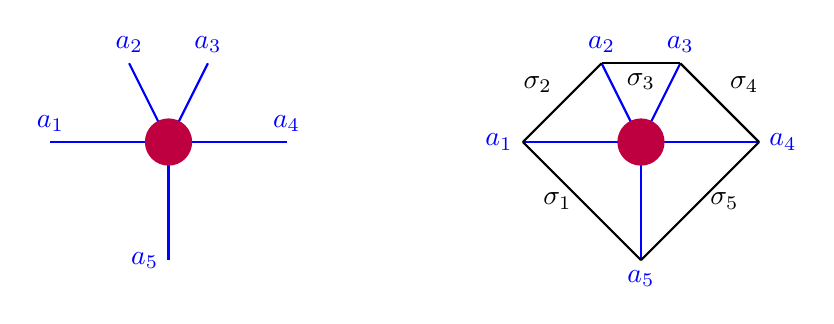
\begin{tikzpicture}[scale=1 ]
\begin{scope}[shift={(-3, 0)}]
        % Define center points
        \coordinate (D1) at (0, 1);         % Center for d1
       

        % Define vertices for d1
        \coordinate (A1) at (-1.5, 1);       % Left of d1
        \coordinate (A2) at (-0.5, 2);        % Top of d1
        \coordinate (A3) at (.5, 2);        % Top-right of d1
        \coordinate (A4) at (1.5, 1);        % Right of d1
        \coordinate (A5) at (0, -.5);
        
        

        % Draw blue arrows from d1 to its vertices
        \draw[- , thick, blue] (D1) -- (A1) node[ above ] {$a_1$};
        \draw[- , thick, blue] (D1) -- (A2) node[  above] {$a_2$};
        \draw[- , thick, blue] (D1) -- (A3) node[ above] {$a_3$};
        \draw[- , thick, blue] (D1) -- (A4) node[ above] {$a_4$};
         \draw[- , thick, blue] (D1) -- (A5) node[ left] {$a_5$};
        
 

 % Draw circles for d1, d2, d3, d4
        \fill[thick, purple] (D1) circle (0.3) node {$d_1$};
           \end{scope}


           
       \begin{scope}[shift={( 3, 0)}]
        % Define center points
        \coordinate (D1) at (0, 1);         % Center for d1
       

        % Define vertices for d1
        \coordinate (A1) at (-1.5, 1);       % Left of d1
        \coordinate (A2) at (-0.5, 2);        % Top of d1
        \coordinate (A3) at (.5, 2);        % Top-right of d1
        \coordinate (A4) at (1.5, 1);        % Right of d1
        \coordinate (A5) at (0, -.5);
        
        

        % Draw blue arrows from d1 to its vertices
        \draw[- , thick, blue] (D1) -- (A1) node[ left ] {$a_1$};
        \draw[- , thick, blue] (D1) -- (A2) node[  above] {$a_2$};
        \draw[- , thick, blue] (D1) -- (A3) node[ above] {$a_3$};
        \draw[- , thick, blue] (D1) -- (A4) node[ right] {$a_4$};
         \draw[- , thick, blue] (D1) -- (A5) node[ below] {$a_5$};
        
         
         \draw[thick, black] (A1) -- (A2) node[midway, above left, black] {$\sigma_2$};
        \draw[thick, black] (A2) -- (A3) node[midway, below,black] {$\sigma_3$};
        \draw[thick, black] (A3) -- (A4) node[midway, above right, black] {$\sigma_4$};
        \draw[thick, black] (A4) -- (A5) node[midway, right, black] {$\sigma_5$};
        \draw[thick, black] (A5) -- (A1) node[midway, left, black] {$\sigma_1$};
 

 % Draw circles for d1, d2, d3, d4
        \fill[thick, purple] (D1) circle (0.3) node {$d_1$};
           \end{scope}
    \end{tikzpicture}
    \caption{Single molecule partition}
    \label{fig:circle_arrows_0}
\end{figure}


\noindent 
{\bf Example}: In the following example in Figure \ref{fig:circle_arrows}, we have 
\begin{equation}\label{exn10}
  \textbf{a}=(a_1,a_2,\ldots,a_{10}), \quad \pi=\left\{ \{1,5\}, \{5,7\},\{8,1\}\right\}  
\end{equation} 
Then  $\Gamma_{\textbf{a}}$ has the following structure. The big dots are connected via internal long edges. Locally, each sub-tree containing a red dot ${\cal M}$ and the edges incident to this $\cal M$ matches a tree structure of a single-molecule partition. More precisely, for these 4 local sub-trees, we have  
\begin{align}
 \Gamma^{(top)}\in \;&\;TSP ({\cal P}_{(a_1,a_2,a_3,a_4, c_1)}, (\sigma_1, \sigma_2,\sigma_3,\sigma_4,\sigma_5) , \pi=\emptyset )
 \\\nonumber 
 \Gamma^{(left)}\in \;&\;TSP ({\cal P}_{(a_9,a_{10},c_2,a_8)}, (\sigma_9, \sigma_{10},\sigma_1,\sigma_8) , \pi=\emptyset )
 \\\nonumber  
 \Gamma^{(middle)}\in \;&\;TSP ({\cal P}_{(a_7,c_2,c_1,c_3)}, (\sigma_7, \sigma_8,\sigma_1,\sigma_5) , \pi=\emptyset )
   \\\nonumber   
\Gamma^{(right)}\in \;&\;TSP ({\cal P}_{(a_5,a_6,c_3)}, (\sigma_5, \sigma_6,\sigma_7) , \pi=\emptyset )
\end{align}
Here $c_1$, $c_2$ and $c_3$ are not in the initial tree $\Gamma_{\textbf{a}}$. We only use them to represent the local structure. 
\begin{figure}[ht]
    \centering
    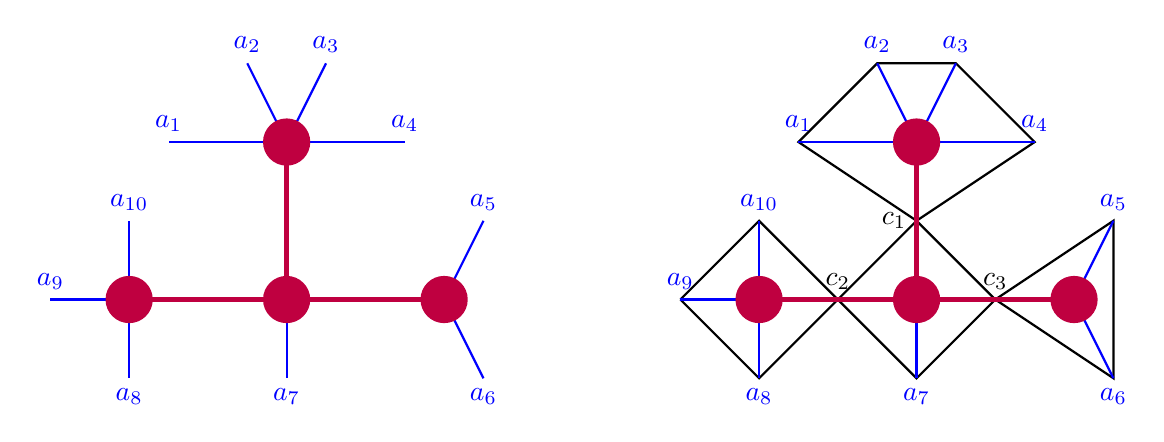
\begin{tikzpicture}[scale=1 ]
\begin{scope}[shift={(-4, 0)}]

        % Define center points
        \coordinate (D1) at (0, 1);         % Center for d1
        \coordinate (D2) at (-2, -1);    % Center for d2
        \coordinate (D3) at (0, -1);       % Center for d3
        \coordinate (D4) at (2, -1);     % Center for d4

        % Define vertices for d1
        \coordinate (A1) at (-1.5, 1);       % Left of d1
        \coordinate (A2) at (-0.5, 2);        % Top of d1
        \coordinate (A3) at (.5, 2);        % Top-right of d1
        \coordinate (A4) at (1.5, 1);        % Right of d1

        % Define vertices for d2
        \coordinate (A8) at (-2 , -2);  % Bottom-left for d2
        \coordinate (A9) at (-3, -1);    % Bottom-center for d2
        \coordinate (A10) at (-2, 0);   % Bottom-left far for d2

        % Define vertices for d3
        \coordinate (A7) at (0, -2);       % Bottom for d3

        % Define vertices for d4
        \coordinate (A5) at (2.5, 0);   % Bottom-right for d4
        \coordinate (A6) at (2.5, -2);     % Bottom-right far for d4

       

        % Draw blue arrows from d1 to its vertices
        \draw[- , thick, blue] (D1) -- (A1) node[ above ] {$a_1$};
        \draw[- , thick, blue] (D1) -- (A2) node[  above] {$a_2$};
        \draw[- , thick, blue] (D1) -- (A3) node[ above] {$a_3$};
        \draw[- , thick, blue] (D1) -- (A4) node[ above] {$a_4$};

        % Draw blue arrows from d2 to its vertices
        \draw[- , thick, blue] (D2) -- (A8) node[below] {$a_8$};
        \draw[- , thick, blue] (D2) -- (A9) node[ above] {$a_9$};
        \draw[- , thick, blue] (D2) -- (A10) node[ above] {$a_{10}$};

        % Draw blue arrows from d3 to its vertex
        \draw[- , thick, blue] (D3) -- (A7) node[below] {$a_7$};

        % Draw blue arrows from d4 to its vertices
        \draw[- , thick, blue] (D4) -- (A5) node[ above] {$a_5$};
        \draw[- , thick, blue] (D4) -- (A6) node[below] {$a_6$};

        % Draw purple arrows connecting the centers
       % \draw[- , ultra thick, purple] (D1) -- (D2);
        \draw[- , ultra thick, purple] (D1) -- (D3);
      %  \draw[- , ultra thick, purple] (D1) -- (D4);
        \draw[- , ultra thick, purple] (D2) -- (D3);
        \draw[- , ultra thick, purple] (D3) -- (D4);

 % Draw circles for d1, d2, d3, d4
        \fill[thick, purple] (D1) circle (0.3) node {$d_1$};
        \fill[thick, purple] (D2) circle (0.3) node {$d_2$};
        \fill[thick, purple] (D3) circle (0.3) node {$d_3$};
        \fill[thick, purple] (D4) circle (0.3) node {$d_4$};
        \end{scope}

        
        \begin{scope}[shift={(4, 0)}]
        % Define center points
        \coordinate (D1) at (0, 1);         % Center for d1
        \coordinate (D2) at (-2, -1);    % Center for d2
        \coordinate (D3) at (0, -1);       % Center for d3
        \coordinate (D4) at (2, -1);     % Center for d4

% Define center points
        \coordinate (C1) at (0, 0);         % Center for C1
        \coordinate (C2) at (-1, -1);    % Center for C2
        \coordinate (C3) at (1, -1);       % Center for C3
        


        % Define vertices for d1
        \coordinate (A1) at (-1.5, 1);       % Left of d1
        \coordinate (A2) at (-0.5, 2);        % Top of d1
        \coordinate (A3) at (.5, 2);        % Top-right of d1
        \coordinate (A4) at (1.5, 1);        % Right of d1

        % Define vertices for d2
        \coordinate (A8) at (-2 , -2);  % Bottom-left for d2
        \coordinate (A9) at (-3, -1);    % Bottom-center for d2
        \coordinate (A10) at (-2, 0);   % Bottom-left far for d2

        % Define vertices for d3
        \coordinate (A7) at (0, -2);       % Bottom for d3

        % Define vertices for d4
        \coordinate (A5) at (2.5, 0);   % Bottom-right for d4
        \coordinate (A6) at (2.5, -2);     % Bottom-right far for d4

        \draw[- , thick, black] (C1)--(A1) -- (A2)--(A3) -- (A4)--(C1) node[ left ] {$c_1$};
        
        \draw[- , thick, black] (C3) -- (A5) -- (A6)--(C3) node[ above] {$c_3$} ;
        
        \draw[- , thick, black]  (C2)--(C1) -- (C3)--(A7) -- (C2)node[ above] {$c_2$} ;
        
        \draw[- , thick, black] (A9) -- (A10)--(C2) -- (A8)--(A9);

        % Draw blue arrows from d1 to its vertices
        \draw[- , thick, blue] (D1) -- (A1) node[ above ] {$a_1$};
        \draw[- , thick, blue] (D1) -- (A2) node[  above] {$a_2$};
        \draw[- , thick, blue] (D1) -- (A3) node[ above] {$a_3$};
        \draw[- , thick, blue] (D1) -- (A4) node[ above] {$a_4$};

        % Draw blue arrows from d2 to its vertices
        \draw[- , thick, blue] (D2) -- (A8) node[below] {$a_8$};
        \draw[- , thick, blue] (D2) -- (A9) node[ above] {$a_9$};
        \draw[- , thick, blue] (D2) -- (A10) node[ above] {$a_{10}$};

        % Draw blue arrows from d3 to its vertex
        \draw[- , thick, blue] (D3) -- (A7) node[below] {$a_7$};

        % Draw blue arrows from d4 to its vertices
        \draw[- , thick, blue] (D4) -- (A5) node[ above] {$a_5$};
        \draw[- , thick, blue] (D4) -- (A6) node[below] {$a_6$};

        % Draw purple arrows connecting the centers
       % \draw[- , ultra thick, purple] (D1) -- (D2);
        \draw[- , ultra thick, purple] (D1) -- (D3);
      %  \draw[- , ultra thick, purple] (D1) -- (D4);
        \draw[- , ultra thick, purple] (D2) -- (D3);
        \draw[- , ultra thick, purple] (D3) -- (D4);

 % Draw circles for d1, d2, d3, d4
        \fill[thick, purple] (D1) circle (0.3) node {$d_1$};
        \fill[thick, purple] (D2) circle (0.3) node {$d_2$};
        \fill[thick, purple] (D3) circle (0.3) node {$d_3$};
        \fill[thick, purple] (D4) circle (0.3) node {$d_4$};
        \end{scope}
    \end{tikzpicture}
    \caption{Multiple molecule Tree}
    \label{fig:circle_arrows}
\end{figure}

\begin{definition}[Definition of $\cal K^{(\pi)}$ and $\Sigma^{(\pi)}$]\label{def_Kpi}
\noindent\textbf{I. Resummation of the kernel $\cal K$.}
Given a subset 
 \begin{equation}\label{defpiij}
  \pi \subset \mathbb Z_n^{off} 
 \end{equation}
we define ${\cal K}^{(\pi)}$ to be the sum of all trees whose long edges are specified by $\pi$, namely
 \begin{equation} 
     {\cal K}^{(\pi)}_{t, \boldsymbol{\sigma}, \textbf{a}} = \sum_{\Gamma_{\textbf{a}}\, \in\,  {TSP}({\cal P}_{\textbf{a}},\; \boldsymbol{\sigma},\; \pi )} \Gamma_{ \textbf{a}}(t, \boldsymbol{\sigma}).
   \end{equation} 
Here $\Gamma_{ \textbf{a}}(t, \boldsymbol{\sigma})$ is defined in Definition \ref{def33}.
Clearly, for $n\ge 2$, 
\begin{equation}\label{KKpi}
  {\cal K}_{t, \boldsymbol{\sigma}, \textbf{a}} =W^{-n+1}\cdot m_{\boldsymbol{\sigma}}\cdot \sum_{\pi}{\cal K}_{t, \boldsymbol{\sigma}, \textbf{a}} ^{(\pi)},\quad m_{\boldsymbol{\sigma}}=\prod_i m_i. 
\end{equation}
Notice that there is a factor $m_{\boldsymbol{\sigma}}W^{-n+1}$ in the last equation due to our convention that $\cal K^{(\pi)}$ is independent of $W$. 

\noindent\textbf{II. Definition of the self-energy.}
We define the self-energy $\Sigma^{(\pi)}$ of ${\cal K}^{(\pi)}$ as follows. Relabel the vertices by letting $d_i$ denote the endpoint of the boundary edge that starts at $a_i$.
When two edges ending at $d_i$ and $d_j$ meet, we identify their endpoints by inserting a Kronecker delta. We label the remaining internal vertices by $s_1,s_2,\ldots$.
The self-energy is obtained by removing the boundary edges from ${\cal K}^{(\pi)}_{t, \boldsymbol{\sigma}, \textbf{a}}$ and summing over all internal indices $s$.
Clearly, we have 
\begin{equation} 
\Sigma^{(\pi)}(t, \boldsymbol{\sigma}, \textbf{d}): 
\quad  
{\cal K}^{(\pi)}_{t, \boldsymbol{\sigma}, \textbf{a}}
=
%\left(\prod_{i=1}^n m_i\right) \cdot 
\sum_{\textbf{d}}\left(\Sigma^{(\pi)}(t, \boldsymbol{\sigma}, \textbf{d})\right)
\cdot 
\prod_{i=1}^n \left(\Theta^{(B)}_{tm_im_{i+1}}\right)_{a_i, d_i}   
\end{equation} 
\end{definition}
 

\noindent 
{\bf Example}: For Figure \ref{fig_n=4} with $n=4$ and 
$\boldsymbol{\sigma}=(+,-,+,-) $, 
$$
\Sigma^{(\emptyset)}(t, \boldsymbol{\sigma}, \textbf{d}) = \delta_{d_1 d_2 d_3 d_4}
+ \delta_{d_1 d_2} \delta_{d_3 d_4} \left(\Theta^{(B)}_{t m^2} - 1\right)_{d_1 d_3}
+ \delta_{d_1 d_4} \delta_{d_2 d_3} \left(\Theta^{(B)}_{t \bar m^2} - 1\right)_{d_1 d_2}.
$$
On the other hand, if  $\boldsymbol{\sigma}=(+,-,+,-)$  then 
$\Sigma^{(\pi)}(t, \boldsymbol{\sigma}, \textbf{d})=0$ if $\pi\ne \emptyset$.


By \eqref{prop:ThfadC} and  explicit calculations,   we have 
$\Sigma^{(\emptyset)}(t, \boldsymbol{\sigma}, \textbf{d}) =O(1) $
and  that $\Sigma^{(\emptyset)}(t, \boldsymbol{\sigma}, \textbf{d})$ is short-ranged in the sense that 
\begin{align}\label{res_SIGempdd}
  \left|\Sigma^{(\emptyset)}(t, \boldsymbol{\sigma}, \textbf{d})\right|\le C_n\exp\left(-c_n \max_{ij}\|d_i-d_j\|\right)   .
\end{align}
In addition,  we have the following sum zero property :
\[
\sum_{d_1, d_2, d_3} \Sigma^{(\emptyset)}(t, \boldsymbol{\sigma}, \textbf{d}) = O(1-t) = O(\eta_t).
\]  
(The name sum zero comes from the fact that the above quantity equals $0$ when $t=1$) 
Due to the translation invariance, the last  bound  is equivalent to 
\[
L^{-1} \cdot \sum_{d_1, d_2, d_3, d_4} \Sigma^{(\emptyset)}(t, \boldsymbol{\sigma}, \textbf{d}) = O(1-t) = O(\eta_t).
\] 
It turns out that this property holds  for all alternating  $\boldsymbol{\sigma}$ with  $\pi=\emptyset$.  

\begin{lemma}[Symmetry and sum zero property]\label{lem:SZ}
For fixed $4 \le n\in 2\mathbb Z$ and an alternating  loop $\boldsymbol{\sigma}^{(alt)}$ with 
\begin{equation}\label{assum_SZ_SinMole}
1\le k\le n, \quad \quad {\sigma}^{(alt)}_k =\begin{cases}
    +, \quad k\in 2\mathbb Z-1
    \\\nonumber
    -, \quad k\in 2\mathbb Z 
\end{cases}\; \;,\quad t\in[0,1]  ,  
\end{equation}
 the single molecule tree graph (i.e., $\pi=\emptyset$) satisfies the following two properties: 
\begin{enumerate}
    \item $\Sigma^{(\emptyset)}(t, \boldsymbol{\sigma}^{(alt)}, \textbf{d}) $ is translationally invariant and 
    symmetric in the sense that 
\[
\Sigma^{(\emptyset)}(t, \boldsymbol{\sigma}^{(alt)}, \textbf{d})
= \Sigma^{(\emptyset)}(t, \boldsymbol{\sigma}^{(alt)}, \textbf{-d})
\]    

\item $\Sigma^{(\emptyset)}(t, \boldsymbol{\sigma}^{(alt)}, \textbf{d}) $ 
has the following sum zero property  
\begin{equation}\label{res_SZ_SinMole}
L^{-1} \cdot\sum_{\textbf{d}\,\in \,\mathbb Z^{n}_L } \Sigma^{(\emptyset)}(t, \boldsymbol{\sigma}^{(alt)}, \textbf{d}) = O(1-t)=O(\eta_t)
\end{equation}
\end{enumerate}
 
\end{lemma}
The sum-zero property is the key input for the  following estimates on $\cal K^{(\pi)}$ and $\cal K$. 
\begin{lemma}[Bound on ${\cal K}$]\label{ML:Kbound+pi}
For any ${\cal K}^{(\pi)}_{t, \boldsymbol{\sigma}, \textbf{a}}$ defined in Definition \ref{def_Kpi},   we have 
\begin{equation}\label{eq:bcal_k_pi}
  {\cal K}^{(\pi)}_{t, \boldsymbol{\sigma}, \textbf{a}} =O_\prec\left((\ell_t \cdot \eta_t)^{-n+1}\right)    
\end{equation}
Together with \eqref{KKpi}, 
we have  
\begin{equation}\label{eq:bcal_k_2}
  {\cal K}_{t, \boldsymbol{\sigma}, \textbf{a}} =O_\prec\left((W \ell_t \cdot \eta_t)^{-n+1}\right)    .
\end{equation}
Notice that there is no $W$ factor in ${\cal K}^{(\pi)}$ due to its definition.
\end{lemma}




\subsection{Proof of Lemma  \ref{lem:SZ}}



\begin{proof}[ Proof of Lemma  \ref{lem:SZ}]
We note that the symmetry and translational-invariance properties are simple consequences of the explicit expression for $\Sigma^{(\pi)}(t, \boldsymbol{\sigma}, \textbf{d})$. We now turn to the sum-zero property.
By   definitions of ${\cal K}^{(\pi)}$ and $\Sigma^{(\pi)}$, for any $n\ge 3$ we have that 
\begin{equation} 
 \sum_{\textbf{a}\,\in \,\mathbb Z^{n}_L } 
{\cal K}^{(\pi)}(t, \boldsymbol{\sigma}, \textbf{a})
= \sum_{\textbf{a}\,\in \,\mathbb Z^{n}_L } \sum_{\textbf{d}\,\in \,\mathbb Z^{n}_L } \prod_{i=1}^n \left(\Theta^{(B)}_{tm_im_{i+1}}\right)_{a_i,d_i}\cdot \Sigma^{(\pi)}(t, \boldsymbol{\sigma}, \textbf{d})    
\end{equation}
Using $S^{(B)} \bf 1 = \bf 1$, we obtain  
$$
\sum_{a_i}\left(\Theta^{(B)}_{tm_im_{i+1}}\right)_{a_i,d_i}=\frac{1}{1-tm_im_{i+1}}.
$$
Therefore, we have 
\begin{equation}\label{KSIGetat}
 \sum_{\textbf{a}\,\in \,\mathbb Z^{n}_L } 
{\cal K}^{(\pi)}(t, \boldsymbol{\sigma}, \textbf{a})
 \Bigg/\sum_{\textbf{d}\,\in \,\mathbb Z^{n}_L } \Sigma^{(\pi)}(t, \boldsymbol{\sigma}, \textbf{d})    \sim \eta_t^{-\big|\{\;i: \;\sigma_i\ne \sigma_{i+1}, \; i\in \mathbb Z_n\}\big|}  .
\end{equation}
By\eqref{KKpi} and   Corollary \ref{lem_sumAinK}, we have  
\begin{align}\label{LKsigm0}
 L^{-1}\cdot \sum_{\pi}\sum_{\textbf{a}\,\in \,\mathbb Z^{n}_L } 
{\cal K}^{(\pi)}(t, \boldsymbol{\sigma}, \textbf{a})= O(\eta_t^{-n+1}).
\end{align}
We now  show that it holds without sum over $\pi$, i.e.,    for  any fixed $\boldsymbol{\sigma}$, $n\ge 3$ and   $\pi$   in \eqref{defpiij}, 
\begin{align}\label{LKsigmas}
%\forall \boldsymbol{\sigma},\; \pi, \; n\ge 3, \quad \quad\quad  
 L^{-1}\cdot \sum_{\textbf{a}\,\in \,\mathbb Z^{n}_L } 
{\cal K}^{(\pi)}(t, \boldsymbol{\sigma}, \textbf{a})=O(\eta_t^{-n+1})  
\end{align}
Assuming that  the last equation  holds in the case that
$\pi=\emptyset$ and $\boldsymbol{\sigma}=\boldsymbol{\sigma}^{(alt)}$, 
  together with \eqref{KSIGetat},   we have 
\begin{equation}
   L^{-1} \cdot \sum_{\textbf{d}\,\in \,\mathbb Z^{n}_L } \Sigma^{(\emptyset)}(t, \boldsymbol{\sigma}^{(alt)}, \textbf{d}) =O(\eta_t).
\end{equation}
This  implies the desired result \eqref{res_SZ_SinMole}. 

We now prove \eqref{LKsigmas} by  induction. If $n=3$, then $\pi$ can only be $\emptyset$. Hence \eqref{LKsigm0} implies \eqref{LKsigmas} in the case $n=3$. Next, we assume that \eqref{LKsigmas} holds with \( n \) replaced by \( m < n \). Under this assumption, we first prove that if  $\pi\ne \emptyset$ then \eqref{LKsigmas} holds, i.e., 
\begin{align} 
 \pi\ne\emptyset\implies  L^{-1}\cdot \sum_{\textbf{a}\,\in \,\mathbb Z^{n}_L } 
{\cal K}^{(\pi)}(t, \boldsymbol{\sigma}, \textbf{a})=O(\eta_t^{-n+1})  
\end{align}
If $\pi\ne \emptyset$, we can always represent 
$ 
{\cal K}^{(\pi)}(t, \boldsymbol{\sigma}, \textbf{a})
$ with the molecule structure and the self-energy  $\Sigma^{(\emptyset)}$. For example, for $n=10$ and $\pi$ in \eqref{exn10}, the molecule structure is the one in Figure \ref{fig:circle_arrows}. As shown in Figure \ref{fig:Decp}, let $d_i$ denote the vertex connected to $a_i$ (these vertices are not marked in the figure), and let $c_i$ denote the vertices of edges connecting molecules (i.e., big dots). Then
$$
{\cal K}^{(\pi)}(t, \boldsymbol{\sigma}, \textbf{a})=
\sum_{\textbf{d}}\sum_{\textbf{c}}\left(\prod_{i=1}^{10}\left(\Theta^{(B)}_{tm_im_{i+1}}\right)_{a_id_i}\right)\cdot \prod_{k=1}^3\Big(\Theta_{{t|m|^2}}-1\Big)_{c_{2k-1}c_{2k}}
\cdot
 \prod_{k=1}^4{\Sigma}^{(\emptyset)}(t, \boldsymbol{\sigma}^{(k)}, \textbf{d}^{(k)})
$$
\begin{figure}[ht]
    \centering
    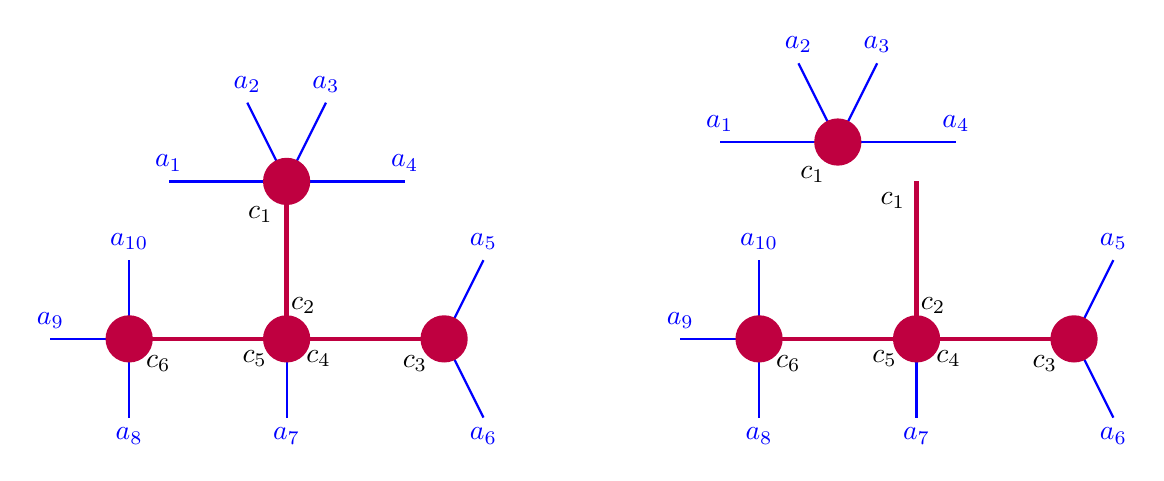
\begin{tikzpicture}[scale=1 ]
\begin{scope}[shift={(-8, 0)}]

        % Define center points
        \coordinate (D1) at (0, 1);         % Center for d1
        \coordinate (D2) at (-2, -1);    % Center for d2
        \coordinate (D3) at (0, -1);       % Center for d3
        \coordinate (D4) at (2, -1);     % Center for d4

        % Define vertices for d1
        \coordinate (A1) at (-1.5, 1);       % Left of d1
        \coordinate (A2) at (-0.5, 2);        % Top of d1
        \coordinate (A3) at (.5, 2);        % Top-right of d1
        \coordinate (A4) at (1.5, 1);        % Right of d1

        % Define vertices for d2
        \coordinate (A8) at (-2 , -2);  % Bottom-left for d2
        \coordinate (A9) at (-3, -1);    % Bottom-center for d2
        \coordinate (A10) at (-2, 0);   % Bottom-left far for d2

        % Define vertices for d3
        \coordinate (A7) at (0, -2);       % Bottom for d3

        % Define vertices for d4
        \coordinate (A5) at (2.5, 0);   % Bottom-right for d4
        \coordinate (A6) at (2.5, -2);     % Bottom-right far for d4

       

        % Draw blue arrows from d1 to its vertices
        \draw[- , thick, blue] (D1) -- (A1) node[ above ] {$a_1$};
        \draw[- , thick, blue] (D1) -- (A2) node[  above] {$a_2$};
        \draw[- , thick, blue] (D1) -- (A3) node[ above] {$a_3$};
        \draw[- , thick, blue] (D1) -- (A4) node[ above] {$a_4$}
       ; 

        % Draw blue arrows from d2 to its vertices
        \draw[- , thick, blue] (D2) -- (A8) node[below] {$a_8$};
        \draw[- , thick, blue] (D2) -- (A9) node[ above] {$a_9$};
        \draw[- , thick, blue] (D2) -- (A10) node[ above] {$a_{10}$};

        % Draw blue arrows from d3 to its vertex
        \draw[- , thick, blue] (D3) -- (A7) node[below] {$a_7$};

        % Draw blue arrows from d4 to its vertices
        \draw[- , thick, blue] (D4) -- (A5) node[ above] {$a_5$};
        \draw[- , thick, blue] (D4) -- (A6) node[below] {$a_6$};

        % Draw purple arrows connecting the centers
       % \draw[- , ultra thick, purple] (D1) -- (D2);
       \draw[-, ultra thick, purple] (D1) -- (D3)
    node[black, above, xshift=6pt, yshift=5pt] {$c_2$}
    node[black, below left, xshift=-3pt] {$c_5$}
    node[black, below right, xshift=3pt] {$c_4$};
      \draw[-, ultra thick, purple] (D3) -- (D1)
    node[black, below left, xshift=-1pt, yshift=-5pt] {$c_1$};
      %  \draw[- , ultra thick, purple] (D1) -- (D4);
        \draw[- , ultra thick, purple] (D3) -- (D2)node[black, below right, xshift=2pt, yshift=-2pt] {$c_6$};
        \draw[- , ultra thick, purple] (D3) -- (D4)node[black, below left, xshift=-2pt, yshift=-2pt] {$c_3$};

 % Draw circles for d1, d2, d3, d4
        \fill[thick, purple] (D1) circle (0.3) node {$d_1$};
        \fill[thick, purple] (D2) circle (0.3) node {$d_2$};
        \fill[thick, purple] (D3) circle (0.3) node {$d_3$};
        \fill[thick, purple] (D4) circle (0.3) node {$d_4$};
        \end{scope}
      \begin{scope}[shift={(0, 0)}]

        % Define center points
        \coordinate (D1) at (-1, 1.5);         % Center for d1
        \coordinate (D2) at (-2, -1);    % Center for d2
        \coordinate (D3) at (0, -1);       % Center for d3
        \coordinate (D4) at (2, -1); 
          \coordinate (D5) at (0, 1);% Center for d4

        % Define vertices for d1
        \coordinate (A1) at (-2.5, 1.5);       % Left of d1
        \coordinate (A2) at (-1.5, 2.5);        % Top of d1
        \coordinate (A3) at (-.5, 2.5);        % Top-right of d1
        \coordinate (A4) at ( .5, 1.5);        % Right of d1

        % Define vertices for d2
        \coordinate (A8) at (-2 , -2);  % Bottom-left for d2
        \coordinate (A9) at (-3, -1);    % Bottom-center for d2
        \coordinate (A10) at (-2, 0);   % Bottom-left far for d2

        % Define vertices for d3
        \coordinate (A7) at (0, -2);       % Bottom for d3

        % Define vertices for d4
        \coordinate (A5) at (2.5, 0);   % Bottom-right for d4
        \coordinate (A6) at (2.5, -2);     % Bottom-right far for d4

       

        % Draw blue arrows from d1 to its vertices
        \draw[- , thick, blue] (D1) -- (A1) node[ above ] {$a_1$};
        \draw[- , thick, blue] (D1) -- (A2) node[  above] {$a_2$};
        \draw[- , thick, blue] (D1) -- (A3) node[ above] {$a_3$};
        \draw[- , thick, blue] (D1) -- (A4) node[ above] {$a_4$}
       ;  \draw[- , thick, blue] (A4) -- (D1)
    node[black, below left, xshift=-1pt, yshift=-5pt] {$c_1$};

        % Draw blue arrows from d2 to its vertices
        \draw[- , thick, blue] (D2) -- (A8) node[below] {$a_8$};
        \draw[- , thick, blue] (D2) -- (A9) node[ above] {$a_9$};
        \draw[- , thick, blue] (D2) -- (A10) node[ above] {$a_{10}$};

        % Draw blue arrows from d3 to its vertex
        \draw[- , thick, blue] (D3) -- (A7) node[below] {$a_7$};

        % Draw blue arrows from d4 to its vertices
        \draw[- , thick, blue] (D4) -- (A5) node[ above] {$a_5$};
        \draw[- , thick, blue] (D4) -- (A6) node[below] {$a_6$};

        % Draw purple arrows connecting the centers
       % \draw[- , ultra thick, purple] (D1) -- (D2);
        \draw[-, ultra thick, purple] (D3) -- (D5)
    node[black, below left] {$c_1$};
       \draw[-, ultra thick, purple] (D5) -- (D3)
    node[black, above, xshift=6pt, yshift=5pt] {$c_2$}
    node[black, below left, xshift=-3pt] {$c_5$}
    node[black, below right, xshift=3pt] {$c_4$};
        %  \draw[- , ultra thick, purple] (D1) -- (D4);
        \draw[- , ultra thick, purple] (D3) -- (D2)node[black, below right, xshift=2pt, yshift=-2pt] {$c_6$};
        \draw[- , ultra thick, purple] (D3) -- (D4)node[black, below left, xshift=-2pt, yshift=-2pt] {$c_3$};

 % Draw circles for d1, d2, d3, d4
        \fill[thick, purple] (D1) circle (0.3) node {$d_1$};
        \fill[thick, purple] (D2) circle (0.3) node {$d_2$};
        \fill[thick, purple] (D3) circle (0.3) node {$d_3$};
        \fill[thick, purple] (D4) circle (0.3) node {$d_4$};
        \end{scope}
    \end{tikzpicture}
    \caption{Decomposition of $\cal K^{(\pi)}$}
    \label{fig:Decp}
\end{figure}
Here  ${\Sigma}^{(\emptyset)}(t, \boldsymbol{\sigma}^{(k)}, \textbf{d}^{(k)})$, $1\le k\le 4$, 
represent the four self-energies   (i.e., four big dots, top, bottom, left, right). More precisely,  
$$
\textbf{d}^{(top)}=(c_1,d_1,d_2,d_3,d_4),\quad
\textbf{d}^{(left)}=(c_6,d_8,d_9,d_{10}),\quad
\textbf{d}^{(bottom)}=(c_2,c_4,d_7,c_5),\quad
\textbf{d}^{(right)}=(c_3,d_5,d_6),\quad
$$
and   $\cal K^{(\pi)}$ is decomposed  into three parts: 
\begin{itemize}
    \item Edges incident to external vertices, i.e., the (blue) boundary edges.
    \item Edges connecting two different molecules, each weighted by $\left(\Theta_{{t|m|^2}}-1\right)$.
    \item The cores ${\Sigma}^{(\emptyset)}(t, \boldsymbol{\sigma}^{(k)}, \textbf{d}^{(k)})$ of the individual molecules.
\end{itemize}






One can easily extend it to the general cases. Given a set 
$\pi$ (which can be the empty set), we label all vertices of long internal edges for $\pi$ by $c_i$, $(1\le i\le 2|\pi|)$. Recall that the vertex connecting with the 
boundary vertex $a_i$ is denoted by  $d_i$. We now denote all internal vertices other than $d_i, c_j$ by $s_k$. 
The index set for $k$ has fewer than $n$ elements, but we will not specify it.
We now explain how to construct the molecule and their tree structure. Given $ \{i, j \} \in \pi$, we draw a line in the polygon from the center of edge $i$ to 
that of $j$.  In this way, we have a partition of the polygon. The set $\pi$ for which there is $\Gamma_{\textbf{a}}$ such that $ {\cal F}_{\mathrm{long}}(\Gamma_{\textbf{a}}, \boldsymbol{\sigma})=\pi $ satisfies that these lines representing the pairing are non-crossing. From now on, we will call $\pi$ a noncrossing pairing. 
Given a non-crossing pairing, we divide the polygon into several regions, say, $M$ regions (note that $M=|\pi|+1$). We represent each region by a big dot (molecule), and there is an edge connecting two dots if and only if these two regions are neighboring.    Notice that each dot typically has many vertices connecting to it, as shown in Figure \ref{fig:clockwise-decagon}. 
\usetikzlibrary{calc}
\begin{figure}[ht]
    \centering 
  \begin{tikzpicture}[scale=0.8]

   %first one
   \begin{scope} 
  
    % Define the radius of the circle
    \def\radius{2.5}
    \def\labeldist{0.3} % Distance of the labels from the vertices

    % Loop to place the 10 nodes and label them
    \foreach \i [evaluate=\i as \angle using {144 - (\i-1)*36}] in {1,...,10} {
        % Place the vertex
        \node (A\i) at ({\angle}:\radius) {};
        % Add the label slightly offset from the vertex
        \node at ({\angle}:{\radius + \labeldist}) {\(a_{\i}\)};
   
     \fill[black] ({\angle}:\radius) circle[radius=0.06];
     }
    
    
    % Draw the polygon by connecting the nodes
    \foreach \i [count=\j from 2] in {1,...,9} {
        \draw [thick] (A\i) -- (A\j);
    }
    \draw [thick] (A10) -- (A1); % Connect the last node to the first

    \usetikzlibrary{calc}
    % Calculate the midpoints of a_1a_10 and a_3a_4
    \coordinate (M1) at ($ (A1)!0.5!(A10) $);
    \coordinate (M2) at ($ (A4)!0.5!(A5) $);
    \coordinate (M3) at ($ (A6)!0.5!(A7) $);
    \coordinate (M4) at ($ (A7)!0.5!(A8) $);

    \coordinate (N1) at (0.4,-0.4);
    \coordinate (N2) at (-1,-1);
    \coordinate (N3) at (1.7,-0.6);
    \coordinate (N4) at (0,1.6);

    % Draw a curve connecting the midpoints
    \draw[black, thick, bend left=10] (M1) to (M2);
    \draw[black, thick, bend right=60] (M2) to (M3);
    \draw[black, thick, bend right=45] (M4) to (M1);

   
 

 % Add a big red dot in the middle of the graph
    \fill[purple] (N1) circle[radius=0.4];
    \fill[purple] (N2) circle[radius=0.4];
    \fill[purple] (N3) circle[radius=0.4];
    \fill[purple] (N4) circle[radius=0.4];
     
   \end{scope} 

   %second one
     \begin{scope}[xshift=8cm]
  
    % Define the radius of the circle
    \def\radius{2.5}
    \def\labeldist{0.3} % Distance of the labels from the vertices

    % Loop to place the 10 nodes and label them
    \foreach \i [evaluate=\i as \angle using {144 - (\i-1)*36}] in {1,...,10} {
        % Place the vertex
        \node (A\i) at ({\angle}:\radius) {};
        % Add the label slightly offset from the vertex
        \node at ({\angle}:{\radius + \labeldist}) {\(a_{\i}\)};
     \fill[black] ({\angle}:\radius) circle[radius=0.06];}
    
    
    % Draw the polygon by connecting the nodes
    \foreach \i [count=\j from 2] in {1,...,9} {
        \draw [thick] (A\i) -- (A\j);
    }
    \draw [thick] (A10) -- (A1); % Connect the last node to the first

    
    % Calculate the midpoints of a_1a_10 and a_3a_4
    \coordinate (M1) at ($ (A1)!0.5!(A10) $);
    \coordinate (M2) at ($ (A4)!0.5!(A5) $);
    \coordinate (M3) at ($ (A6)!0.5!(A7) $);
    \coordinate (M4) at ($ (A7)!0.5!(A8) $);

    \coordinate (N1) at (0.4,-0.4);
    \coordinate (N2) at (-1,-1);
    \coordinate (N3) at (1.7,-0.6);
    \coordinate (N4) at (0,1.6);

    % Draw a curve connecting the midpoints
    \draw[black, thick, bend left=10] (M1) to (M2);
    \draw[black, thick, bend right=60] (M2) to (M3);
    \draw[black, thick, bend right=45] (M4) to (M1);

   


 \draw[red, thick ] (N1) to (N2);
 \draw[red, thick] (N4) to (N1);
 \draw[red, thick ] (N3) to (N1);

 \draw[blue, thick ] (N1) to (A7);
\draw[blue, thick ] (N2) to (A8);
\draw[blue, thick ] (N2) to (A9);
\draw[blue, thick ] (N2) to (A10);
 \draw[blue, thick ] (N3) to (A5);
  \draw[blue, thick ] (N3) to (A6);
     \draw[blue, thick ] (N4) to (A1);
     \draw[blue, thick ] (N4) to (A2);
     \draw[blue, thick ] (N4) to (A3);
     \draw[blue, thick ] (N4) to (A4);

 % Add a big red dot in the middle of the graph
   \fill[purple] (N1) circle[radius=0.4];
    \fill[purple] (N2) circle[radius=0.4];
    \fill[purple] (N3) circle[radius=0.4];
    \fill[purple] (N4) circle[radius=0.4];
       
   \end{scope} 
    \end{tikzpicture}
    \caption{$\pi=\left\{ \{1,5\}, \{5,7\},\{8,1\}\right\} $ }
     \label{fig:clockwise-decagon}
\end{figure}


In general, there are complicated structures inside these molecules; there are short edges and other vertices labeled by $s_k$. All vertices labeled by $s_k$
 are required to be summed. 
With this convention,  for $\pi$  with   $M$ molecules, we can write 
\begin{align}\label{KThThSigma}
{\cal K}^{(\pi)}(t, \boldsymbol{\sigma}, \textbf{a})= 
\sum_{\textbf{d}}\sum_{\textbf{c}}\left(\prod_{i=1}^{n} \left(\Theta^{(B)}_{tm_im_{i+1}}\right)_{a_id_i}\right)\cdot \prod_{k=1}^{M-1}\Big(\Theta_{{t|m|^2}}-1\Big)_{c_{2k-1}c_{2k}}
\cdot
 \prod_{k=1}^{M}{\Sigma}^{(\emptyset)}(t, \boldsymbol{\sigma}^{(k)}, \textbf{d}^{(k)})   
\end{align}
Here the vertices labelled by $s_k$ are summed and thus they no longer appear explicitly in the formula above. 
Summing over  $\textbf{a}$,  we have 
\begin{align}\label{sumkpitsa}
\sum_{\textbf{a}}{\cal K}^{(\pi)}(t, \boldsymbol{\sigma}, \textbf{a})=
\sum_{\textbf{a},\,\textbf{d},\,\textbf{c}}\left(\prod_{i=1}^{n}  \left(\Theta^{(B)}_{tm_im_{i+1}}\right)_{a_id_i}\right)\cdot \prod_{k=1}^{M-1}\Big(\Theta_{{t|m|^2}}-1\Big)_{c_{2k-1}c_{2k}}
\cdot
 \prod_{k=1}^{M}{\Sigma}^{(\emptyset)}(t, \boldsymbol{\sigma}^{(k)}, \textbf{d}^{(k)})   
\end{align}
 Given a molecule structure (or equivalently a set $\pi$ representing non-crossing pairings), there must be a molecule  containing just one $c$ vertex, i.e., the big dot for this molecule  connects to only  one  $\big(\Theta^{(B)}_{t|m|^2}-1\big)_{c_{2k-1},c_{2k}}$ edge. (For example, the top, left and right molecules in Figure \ref{fig:Decp}). 
  In a different language, this molecule represents a region with exactly  one  pairing line.  
For simplicity, we assume that it is the first molecule  containing  $c_1$ and  connecting  with $a_1,a_2,\ldots,a_{m-1}$. 
With these notations, we have 
\begin{equation} \label{jjshsaa0}
\{1,m \}\in \pi, \quad \sigma_1\ne \sigma_{m }
\end{equation}
The expression in the formula of ${\cal K}^{(\pi)}$ related to this molecule is 
$$
\sum_{d_1,\cdots, d_{m-1}}\Sigma^{(\emptyset)}\Bigg(t, (\sigma_1,\ldots,\sigma_m), (d_1,\cdots, d_{m-1}, c_1)\Bigg)\cdot  \left(\prod_{i=1}^{m-1} \left(\Theta^{(B)}_{tm_im_{i+1}}\right)_{a_id_i}\right) 
$$
(For example: the top right part in Figure \ref{fig:Decp} is for the case $m=5$.) Notice that  $d_i, a_i, 1\le i\le m-1 $ do not  appear in other molecules.  The following part is separated  from  other parts in \eqref{sumkpitsa}, i.e., 
 $$
f^*(c_1):=\sum_{a_1,\cdots, a_{m-1}}\sum_{d_1,\cdots, d_{m-1}}\Sigma^{(\emptyset)}\Bigg(t, (\sigma_1,\ldots,\sigma_m), (d_1,\cdots, d_{m-1}, c_1)\Bigg)\cdot  \left(\prod_{i=1}^{m-1}\left(\Theta^{(B)}_{tm_im_{i+1}}\right)_{a_id_i}\right) 
$$
Now we can write the $\cal K^{(\pi)}$ in \eqref{sumkpitsa} in the terms of $f^*(c_1)$ as follows: 
\begin{align}\label{sumkp2itsa2}
\sum_{\textbf{a}}{\cal K}^{(\pi)}(t, \boldsymbol{\sigma}, \textbf{a})=& \sum_{c_1} f^*(c_1)\cdot  
\sum_{a_m,\cdots , a_n}
\sum_{d_m,\cdots , d_n}
\sum_{c_2,\cdots,c_{2M-2}}\\\nonumber
&\left(\prod_{i=m}^{n}\left(\Theta^{(B)}_{tm_im_{i+1}}\right)_{a_id_i}\right)\cdot \prod_{k=1}^{M-1}\Big(\Theta_{{t|m|^2}}-1\Big)_{c_{2k-1}c_{2k}}
\cdot
 \prod_{k=2}^{M}{\Sigma}^{(\emptyset)}(t, \boldsymbol{\sigma}^{(k)}, \textbf{d}^{(k)})   
\end{align}
In the Figure \ref{fig:Decp}, the upper right part represents the $f ^*(c_1)$ and the lower right part represents the 2nd line of the \eqref{sumkp2itsa2}. 

By translation invariance, $f^*(c_1)$ does not depend on $c_1$, i.e.,
$f^*(c_1)= f^*(1)\in \mathbb C$.
Inserting it  back to \eqref{sumkp2itsa2}, we obtain that
\begin{align}\label{sumkp3itsa3}
\sum_{\textbf{a}}{\cal K}^{(\pi)}(t, \boldsymbol{\sigma}, \textbf{a})=f^*(1) &\cdot  
\sum_{a_m,\cdots , a_n}\;
\sum_{d_m,\cdots , d_n}\;
\sum_{\textbf{c}}\\\nonumber
&\left(\prod_{i=m}^{n}\left(\Theta^{(B)}_{tm_im_{i+1}}\right)_{a_id_i}\right)\cdot \prod_{k=1}^{M-1}\Big(\Theta_{{t|m|^2}}-1\Big)_{c_{2k-1}c_{2k}}
\cdot
 \prod_{k=2}^{M}{\Sigma}^{(\emptyset)}(t, \boldsymbol{\sigma}^{(k)}, \textbf{d}^{(k)})   
\end{align}
Since   $c_1$  appears only  in the internal edge $ (\Theta_{{t|m|^2}}-1 )_{c_1c_2}$, we can sum over $c_1$. By definition of 
$\Theta_{{t|m|^2}}$,  $S^{(B)} \bf 1 = \bf 1$ and $|m|=1$, we have 
$$  \sum_{a}\left(\Theta_{t|m|^2}-1\right)_{ab}= \frac t { 1-t} =t \sum_{a}\left(\Theta_{t|m|^2}\right)_{ab}
$$

Thus  we can replace $(\Theta^{(B)}_{t|m|^2}-1)_{c_1c_2}$ in \eqref{sumkp3itsa3} with $t(\Theta^{(B)}_{t|m|^2})_{c_1c_2}$.  
This replacement shows that after  summing  over $c_1$, the internal edge $c_1-c_2$ becomes an external edge with a factor $t$. This will be crucial later on when we split the graph.  We can now rewrite 
\begin{align}\label{sumkp4itsa4}
\sum_{\textbf{a}}{\cal K}^{(\pi)}(t, \boldsymbol{\sigma}, \textbf{a}) \;=\;&t\cdot f^*(1) \cdot  
\sum_{a_m,\cdots , a_n}\;
\sum_{d_m,\cdots , d_n}\;
\sum_{\textbf{c}}\\\nonumber
&\left(\prod_{i=m}^{n}\left(\Theta^{(B)}_{tm_im_{i+1}}\right)_{a_id_i}\right)\cdot 
\left(\Theta^{(B)}_{t|m|^2}\right)_{c_1c_2}
\prod_{k=2}^{M-1}\Big(\Theta_{{t|m|^2}}-1\Big)_{c_{2k-1}c_{2k}}
\cdot
 \prod_{k=2}^{M}{\Sigma}^{(\emptyset)}(t, \boldsymbol{\sigma}^{(k)}, \textbf{d}^{(k)})   
\end{align}
  Define $\pi'$ to be $\pi$ with the pair for edge $\{c_1, c_2\}$ removed, i.e. 
  $$
  \pi'=\pi\setminus\{\{1,m\}\}
  $$
  Denote 
$$
\boldsymbol{\sigma}'=(\sigma_1,  \,\sigma_{m}, \,\sigma_{m+1}, \,\cdots  \,\sigma_{n}) ,\quad \textbf{a}'=(c_1, \,a_{m},\,a_{m+1},\,\cdots\, a_{n})
$$
%As show in the right hand side  of  Figure \ref{fig:Decp}, there exists $\pi'$ s.t. the r.h.s of \eqref{sumkp4itsa4} can written in terms of $\cal K^{(\pi')}$. More precisely
Then we have (see  Figure \ref{fig:Decp} for an example) 
\begin{align}\label{sumkp5itsa5}
\sum_{\textbf{a}}{\cal K}^{(\pi)}(t, \boldsymbol{\sigma}, \textbf{a})=t\cdot f^*(1) &\cdot  
\sum_{\textbf{a}'}{\cal K}^{(\pi')}(t, \boldsymbol{\sigma}', \textbf{a}') 
\end{align} 
Notice that   $\{c_1, c_2\}$  is  a boundary  edge in  
$\mathcal{K}^{\left(\pi^{\prime}\right)}\left(t, \boldsymbol{\sigma}^{\prime}, \mathbf{a}^{\prime}\right)$ and it needs to be of the form $\left(\Theta_{t|m|^2}^{(B)}\right)_{c_1 c_2}$.
Since $\textbf{a}'\in \mathbb Z_L^{n-m+2}$, we can apply the induction hypothesis  \eqref{LKsigmas} to  ${\cal K}^{(\pi')}$. Thus 
\begin{align}\label{sumkp6itsa6}
\sum_{\textbf{a}}{\cal K}^{(\pi)}(t, \boldsymbol{\sigma}, \textbf{a})= {O(t\cdot f^*(1) \cdot L\cdot (\eta_t)^{-n+m-1})}
\end{align}


%{Now we estimate $f^*(1)$} by m
Multiplying  $(\Theta^{(B)}_{t|m|^2})_{c_1,a}=(\Theta^{(B)}_{tm_1m_m})_{c_1,a}$ to   $f^*(c_1)$ and summing up $c_1$ and $a$,  we obtain 
\begin{align}\label{sumkp7itsa7}
   & \sum_{a}\sum_{c_1}(\Theta^{(B) }_{tm_1m_m})_{c_1 ,a}\cdot f^*(c_1)
    \\\nonumber
     =& \sum_{a,\,c_1}\;\sum_{a_1,\cdots, a_{m-1}}\sum_{d_1,\cdots, d_{m-1}}\Sigma^{(\emptyset)}\Bigg(t, (\sigma_1,\ldots,\sigma_m), (d_1,\cdots, d_{m-1}, c_1)\Bigg)\cdot  \left(\prod_{i=1}^{m-1}\left(\Theta^{(B)}_{tm_im_{i+1}}\right)_{a_id_i}\right)(\Theta^{(B) }_{tm_1m_m})_{c_1 ,a} 
\end{align}
By definition, the right hand side  can be written in terms of  ${\cal K}^{(\emptyset)} \big(t, (\sigma_1,\ldots,\sigma_m), (a_1,\cdots, a_{m-1}, a)\big)$, namely, 
\begin{align}\label{jyya}
 \sum_a\sum_{c_1}f^*(c_1)(\Theta^{(B) }_t)_{c_1,a}&=\sum_{a_1,\cdots, a_{m-1},\;a}{\cal K}^{(\emptyset)} \Bigg(t, (\sigma_1,\ldots,\sigma_m), (a_1,\cdots, a_{m-1}, a)\Bigg) .
\end{align}
By the induction hypothesis \eqref{LKsigmas}, the right-hand side of \eqref{jyya} is $O(L\cdot\eta_t^{-m+1})$. Thus
\begin{align}\label{jyasdfya}
\sum_a\sum_{c_1}f^*(c_1)(\Theta^{(B) }_t)_{c_1,a} = O(L\cdot\eta_t^{-m+1})
\end{align}
On the other hand, since $f^*(c_1)=f^*(1)$, we have the identity 
\begin{align}
\sum_a\sum_{c_1}f^*(c_1)(\Theta^{(B) }_t)_{c_1,a}=L\cdot f^*(1)\cdot (1-t)^{-1}.
\end{align}
Hence
 $$
  f^*(c_1)=f^*(1)=O(\eta_t^{-m+2}) $$
Together with \eqref{sumkp6itsa6}, we have proved   \eqref{LKsigmas}  if  $\pi\ne \emptyset$.  


For  $\pi=\emptyset$, we write ${\cal K}^{(\emptyset)}$  as
\begin{align}\label{LKsigmasES}
 \sum_{\textbf{a}\,\in \,\mathbb Z^{n}_L } 
{\cal K}^{(\emptyset)}(t, \boldsymbol{\sigma}, \textbf{a})
=
 \sum_{\pi}\sum_{\textbf{a}\,\in \,\mathbb Z^{n}_L } 
{\cal K}^{(\pi)}(t, \boldsymbol{\sigma}, \textbf{a})
-
\sum_{\pi\ne\emptyset}  \sum_{\textbf{a}\,\in \,\mathbb Z^{n}_L } 
{\cal K}^{(\pi)}(t, \boldsymbol{\sigma}, \textbf{a}) 
=
  O(L\cdot \eta_{t}^{-n+1}) 
\end{align}
Here  we have used \eqref{LKsigm0} to bound the first term on the right hand side and  \eqref{LKsigmas} for the second term. 
We  have thus proved  \eqref{LKsigmas} and Lemma \ref{lem:SZ}. 
 
\end{proof} 

\subsection{Proof of Lemma   \ref{ML:Kbound+pi}}

\begin{proof}[Proof of Lemma  \ref{ML:Kbound+pi}]
 We first focus on the case $\pi=\emptyset$. By symmetry, without loss of generality, we can split it into three cases
 \begin{enumerate}
     \item Pure loop, i.e., $\sigma_k=+$ for all $1\le k\le n$ or  $\sigma_k=-$ for all $1\le k\le n$. In this case, all edges are short edges, hence we can easily obtain \eqref{eq:bcal_k_pi}. 
     \item $\sigma_1=+$, $\sigma_2=-$, and  there exists $j$ s.t. $\sigma_j=\sigma_{j+1}=+$. 
    \item $\boldsymbol{\sigma}$ is alternating as in \eqref{assum_SZ_SinMole}, i.e. $\boldsymbol{\sigma}=\boldsymbol{\sigma}^{(alt)}$. 
 \end{enumerate}
  Recall  that for $\sigma_1\ne\sigma_2$, and $\pi=\emptyset$, we have 
\begin{align*}
{\cal K}^{(\emptyset)}_{t, \boldsymbol{\sigma}, \textbf{a}}
=\;&
 \sum_{\textbf{d}}\left(\Sigma^{(\emptyset)}(t, \boldsymbol{\sigma}, \textbf{d})\right)
\cdot 
\prod_{i=1}^n \left(\Theta^{(B)}_{tm_im_{i+1}}\right)_{a_i, d_i}
\\\nonumber
=\;&\sum_{d_1}\left(\Theta^{(B)}_{t|m|^2}\right)_{a_1, d_1}
\cdot \sum_{d_2,\,\cdots,\, d_n}\left(\Sigma^{(\emptyset)}(t, \boldsymbol{\sigma}, \textbf{d})\right)
\cdot 
\prod_{i=2}^n \left(\Theta^{(B)}_{tm_im_{i+1}}\right)_{a_i, d_i}  
\end{align*}
We are going to prove the following statement, which is  slightly stronger than \eqref{eq:bcal_k_pi}:
\begin{align}\label{spwow3}
    \sum_{d_2,\,\cdots,\, d_n}\left(\Sigma^{(\emptyset)}(t, \boldsymbol{\sigma}, \textbf{d})\right)
\cdot 
\prod_{i=2}^n \left(\Theta^{(B)}_{tm_im_{i+1}}\right)_{a_i, d_i}
=O((\ell_t\eta_t)^{-n+2})\cdot \left(\min_{2\le k\le n} \|a_k-d_1\|+1\right)^{-1}
\end{align}
First, if there exists $2\le j\le n$ s.t.  $\sigma_j=\sigma_{j+1}=+$, then  \eqref{prop:ThfadC} shows that  
$$
\left(\Theta^{(B)}_{tm_jm_{j+1}}\right)_{a_j, d_j}= \left(\Theta^{(B)}_{tm^2}\right)_{a_j, d_j}=O(1)
$$
It implies that
$$
\prod_{i=2}^n \left(\Theta^{(B)}_{tm_im_{i+1}}\right)_{a_i, d_i}=O((\ell_t\eta_t)^{-n+2})
$$
On the other hand, due to the short range property of $\Sigma^{(\emptyset)}(t, \boldsymbol{\sigma}, \textbf{d})$ (in \eqref{res_SIGempdd}), we have
$$
\left|\sum_{d_2,\,\cdots,\, d_n}\left(\Sigma^{(\emptyset)}(t, \boldsymbol{\sigma}, \textbf{d})\right)
\cdot 
\prod_{i=2}^n \left(\Theta^{(B)}_{tm_im_{i+1}}\right)_{a_i, d_i}\right|\le C \prod_{i=2}^n \left\|\Theta^{(B)}_{tm_im_{i+1}}\right\|_{\max}
$$
By combining these two bounds, we derive \eqref{spwow3} for this case.


Next we prove \eqref{spwow3}  in the case that $\pi=\emptyset$ and $\boldsymbol{\sigma}=\boldsymbol{\sigma}^{(alt)}$. 
In this case, 
$$
\prod_{i=2}^n \left(\Theta^{(B)}_{tm_im_{i+1}}\right)_{a_i, d_i}
=
\prod_{i=2}^n \left(\Theta^{(B)}_{t|m|^2}\right)_{a_i, d_i} 
$$
With short range property of $\Sigma^{(\emptyset)}(t, \boldsymbol{\sigma}, \textbf{d})$ (in \eqref{res_SIGempdd}), and the estimate of $(\Theta^{(B)}_{t|m|^2})_{a_id_i}$  in \eqref{prop:ThfadC}, one can easily bound the left-hand side of \eqref{spwow3} by 
$ 
  O((\ell_t\eta_t)^{-n+1}) 
$. To obtain the missing factor for \eqref{spwow3}, we need to apply the sum zero property which  we proved in Lemma \ref{lem:SZ}, i.e., 
\begin{equation}\label{SZjadljsk}
   \sum_{d_2,\,\cdots,\,d_n}\left(\Sigma^{(\emptyset)}(t, \boldsymbol{\sigma}, \textbf{d})\right)=O(\eta_t) 
\end{equation}
Here we use the translation invariance of \(\Sigma^{(\emptyset)}\). More precisely, the left-hand side of \eqref{SZjadljsk}
is independent of \(d_1\). Hence the full sum over \(d_1,\ldots,d_n\) is \(L\) times this partial sum. Lemma~\ref{lem:SZ}, applied to the full sum, therefore yields \eqref{SZjadljsk}.  For simplicity, for fixed $d_1$ and $\textbf{a}$, we temporarily denote $s$, $f$ and $g$ as follows 
$$
s_i:=d_i-d_1,\quad \quad f(a_i, s_i):=\left(\Theta^{(B)}_{t|m|^2}\right)_{a_i,(d_1+s_i)}, \quad g(s_2, \cdots,s_n):=\Sigma^{(\emptyset)}(t, \boldsymbol{\sigma}, \textbf{d})$$
Then the l.h.s. of \eqref{spwow3} can be written as 
\begin{align} \label{Kfadgd}
 \sum_{d_2,\,\cdots,\, d_n}\left(\Sigma^{(\emptyset)}(t, \boldsymbol{\sigma}, \textbf{d})\right)
\cdot 
\prod_{i=2}^n \left(\Theta^{(B)}_{tm_im_{i+1}}\right)_{a_i, d_i}
= \sum_{s_2\,\cdots,\,s_n} \prod_{i=2}^nf(a_i, s_i)\cdot g(\textbf{s})
\end{align}
Note due the fast decay of $g(\textbf{s})$, we can focus on the case that $\max_i|s_i|\prec 1$. 
 By Lemma~\ref{lem:SZ},  we have 
$$
g(\textbf{s})=g(-\textbf{s}), \quad 
 \sum_{s_2,\,\cdots,\,s_n} g(s_2, \cdots,s_n) = O(\eta_t).
$$ 
For each $i$, we write 
$$
f(a_i, s_i)=f_0(a_i,s_i)+f_1(a_i,s_i )+f_2(a_i,s_i)
$$
where 
\begin{align}
f_0(a_i,s_i)=&f(a_i,0)
\\\nonumber
f_1(a_i,s_i)=&\frac12\left(f(a_i,s_i)-f(a_i, -s_i)\right)  
\\\nonumber
f_2(a_i,s_i)=&f(a_i,s_i)-f(a_i,0)-\frac12\left(f(a_i,s_i)-f(a_i,-s_i)\right)  
\end{align}
%Use  $$
%f(x-y)=\sum_{k=0}^\infty \left(tS^{(B)}\right)^k_{xy}$$
%and  the smoothness of random walk, we have 
By Lemma \ref{lem_propTH}
\begin{align}
f_0(a_i,s_i)=&O((\ell_t\eta_t)^{-1}), 
\\\nonumber
f_1(a_i,s_i)=&O(\ell_t^{-1}\eta_t^{-1/2}),
\\\nonumber
f_2(a_i,s_i)=&O((\|a_i-d_1\|+1)^{-1}) .
\end{align}
Inserting 
$$\prod_if(a_i,s_i)=\prod_i \left(f_0(a_i,s_i)+f_1(a_i,s_i)+f_2(a_i,s_i)\right)$$
into \eqref{Kfadgd}, we obtain 
\begin{align} \label{Kfs2dgd}
 \sum_{d_2,\,\cdots,\, d_n}\left(\Sigma^{(\emptyset)}(t, \boldsymbol{\sigma}, \textbf{d})\right)
\cdot 
\prod_{i=2}^n \left(\Theta^{(B)}_{tm_im_{i+1}}\right)_{a_i, d_i}
= 
\sum_{s_2\,\cdots,\,s_n}\;  \sum_{0\le \xi_2, \,\xi_3, \cdots,  \xi_n \le 2 }\;  \prod_{i=2}^nf_{\xi_i}(a_i, s_i)\cdot g(\textbf{s})
\end{align}
 We claim that for $g$ and $f$ satisfying the estimates just stated and  any fixed $\xi$'s, 
\begin{equation}\label{aauduyuadw}
\sum_{s_2\,\cdots,\,s_n}    \prod_{i=2}^nf_{\xi_i}(a_i, s_i)\cdot g(\textbf{s})= O((\ell_t\eta_t)^{-n+2})\cdot \left(\min_{2\le k\le n} \|a_k-d_1\|+1\right)^{-1} .
\end{equation}


We estimate the l.h.s. in the following cases: 
\begin{itemize}
    \item If $\xi_k=2$ for some $k$, assume without loss of generality that $\xi_n=2$. Then 
    $$
     \prod_{i=2}^nf_{\xi_i}(a_i, s_i)=O\left((\ell_t\eta_t)^{-n+2}\right)\cdot  \|a_n-d_1\|^{-1}
    $$
    It implies that in this case \eqref{aauduyuadw} holds.  
  
\item If $0\le \xi_k\le 1$ for all $2\le k\le n$ and two of the $\xi_k$ are equal to $1$, then, similarly to the previous case, 
$$
    \prod_{i=2}^nf_{\xi_i}(a_i, s_i)=O\left((\ell_t\eta_t)^{-n+1}\right)\cdot \eta_t
    =O\left((\ell_t\eta_t)^{-n+2}\right)\cdot \ell_t^{-1}
    $$
 If $\|a_k-d_1\|=O(\ell_t)$ for all $2 \le k \le n$, this  implies  \eqref{aauduyuadw};   if $\|a_k-d_1\|\gg \ell_t$ for some $2 \le k \le n$, then the l.h.s. of \eqref{aauduyuadw} is  exponentially small. 

    \item If $0\le \xi_k\le 1$ for all $2\le k\le n$ and exactly one of the $\xi_k$ equals $1$, assume without loss of generality that $\xi_n=1$. Similarly to the previous case, 
$$
   \prod_{i=2}^nf_{\xi_i}(a_i, s_i)g(\textbf{s})=
\prod_{i=2}^{n-1}f(a_i,0) f_{1}(a_n,s_n)  g(\textbf{s})
    $$
By definition, we have  
$$
f_{1}(a_n,s_n) =-f_{1}(a_n,-s_n). 
$$
By symmetry and the property $g(\textbf{s})=g(-\textbf{s})$,  the left-hand side of \eqref{aauduyuadw} equals zero in this case. 
    \item At last, if  $\xi_k=0$ for all $2\le k\le n$. Then 
    $$
    \prod_{i=2}^nf_{\xi_i}(a_i, s_i)g(\textbf{s})=
  \prod_{i=2}^{n }f(a_i,0)   g(\textbf{s})
$$
Applying \eqref{SZjadljsk}, we have 
$$
 \sum_{\textbf{s}}g(\textbf{s})=O(\eta_t)
$$
 It implies that in this case \eqref{aauduyuadw} holds. 
\end{itemize}

Therefore, we have proved that for any $\xi$'s, the \eqref{aauduyuadw} holds, which completes the proof of \eqref{spwow3} for the case of $\pi=\emptyset$ and $\sigma_1=+$, $\sigma_2=-$. 

\bigskip

We  now prove  \eqref{eq:bcal_k_pi} in the case $\pi\ne \emptyset$. As above, we use the decomposition method as in Figure \ref{fig:Decp}.  By \eqref{KThThSigma} we write  \begin{align} 
{\cal K}^{(\pi)}(t, \boldsymbol{\sigma}, \textbf{a})=
\sum_{\textbf{d}}\sum_{\textbf{c}}\left(\prod_{i=1}^{n}\left(\Theta^{(B)}_{tm_im_{i+1}}\right)_{a_id_i}\right)\cdot \prod_{k=1}^{M-1}\Big(\Theta_{{t|m|^2}}-1\Big)_{c_{2k-1}c_{2k}}
\cdot
\prod_{k=1}^{M}{\Sigma}^{(\emptyset)}(t, \boldsymbol{\sigma}^{(k)}, \textbf{d}^{(k)})   \end{align}
Here, each molecule contains at least one $c$-vertex; equivalently, each
molecule has degree at least one with respect to the internal $(\Theta-1)$
edges. On the other hand, if every molecule had degree larger than one, then
the molecule graph would contain an internal $(\Theta-1)$-edge cycle,
contradicting its tree structure. Therefore at least one molecule has degree
one, i.e. the big dot corresponding to this molecule connects to only one
$(\Theta^{(B)}_{t|m|^2}-1)_{c_{2k-1},c_{2k}}$ edge. (For example, the top, left and right molecules in Figure \ref{fig:Decp}). For simplicity, we assume that it is the first molecule, and it contains $c_1$ and  connects with $a_1,a_2,\ldots,a_{m-1}$. Note that in this case 
\begin{equation} \label{jjshsaa}
\{1,m \}\in \pi, \quad \sigma_1\ne \sigma_{m }
\end{equation}
As in the r.h.s of Figure \ref{fig:Decp}, we decompose  ${\cal K}^{(\pi)}(t, \boldsymbol{\sigma}, \textbf{a})$ into a  product of two parts,  ${\cal A}$ and ${\cal B}$, such that 
\begin{align} \label{aklsdjfyuadsfyo}
{\cal K}^{(\pi)}(t, \boldsymbol{\sigma}, \textbf{a})
& =
\sum_{c_1} \left({\cal A}_{a_1,\cdots,a_{m-1},c_1}\right)\cdot \left({\cal B}_{c_1, a_m,\cdots,a_{n}}\right)
\\\nonumber
{\cal A}_{a_1,\cdots,a_{m-1},c_1}& =\sum_{d_1,\,\cdots,\,d_{m-1}} \left(\prod_{i=1}^{m-1}\left(\Theta^{(B)}_{tm_im_{i+1}}\right)_{a_id_i}\right)
\cdot
 {\Sigma}^{(\emptyset)}(t, \boldsymbol{\sigma}^{(1)}, \textbf{d}^{(1)}),
 \quad  \textbf{d}^{(1)}  =(d_1,d_2,\ldots,d_{m-1},c_1)  
\\\nonumber
 {\cal B}_{c_1, a_m,\cdots,a_{n}} &=\sum_{d_m,\cdots,d_n}\; \sum_{c_2,\cdots,c_{2M-2}}\left(\prod_{i=m}^{n}\left(\Theta^{(B)}_{tm_im_{i+1}}\right)_{a_id_i}\right)\cdot \prod_{k=1}^{M-1}\Big(\Theta_{{t|m|^2}}-1\Big)_{c_{2k-1}c_{2k}}
\cdot
 \prod_{k=2}^{M}{\Sigma}^{(\emptyset)}(t, \boldsymbol{\sigma}^{(k)}, \textbf{d}^{(k)}). 
\end{align}
Using \eqref{spwow3}, we have 
$$
 {\cal A}_{a_1,\cdots,a_{m-1},c_1}=O((\ell_t\eta_t)^{-m+2})\cdot \left(\min_{1\le k\le m} \|a_k-c_1\|+1\right)^{-1}
$$
On the other hand, with the induction hypothesis and $(\Theta_t-1)_{c_1c_2}=t\left(S^{(B)}\cdot \Theta_t\right)_{c_1c_2}$,   we have 
$$
{\cal B}_{c_1, a_m,\cdots,a_{n}}=O((\ell_t\eta_t)^{-n+m-1})
$$
Combining  these two bounds and inserting  them back to \eqref{aklsdjfyuadsfyo}, we obtain \eqref{eq:bcal_k_pi} for the case that $\pi\ne \emptyset$, and complete the proof of Lemma  \ref{ML:Kbound+pi}

\end{proof}
 





\section{\texorpdfstring{$G$}{G}-entry estimates}
In this section, we bound $G$-entries and 1-loops in terms of 2-loops. The proof of Lemma \ref{lem_GbEXP} uses a time-independent method.
It relies on a standard decomposition widely employed for Wigner matrices (e.g., \cite{erdHos2012rigidity}) and band matrices (e.g., \cite{Average_fluc}).


\begin{lemma}[Resolvent entry estimate]\label{lem_GbEXP}  
Recall   $z_t$ and  $G_t$ (which depend on  $N$ ) from  Definitions \ref{def_flow} and \ref{Def:G_loop}. 
Suppose that $|E| < 2 - \kappa, 0 \leq t <  1$.
For a fixed constant $c > 0$, define the event
\begin{equation}\label{def_asGMc}
    \Omega(t, c) := \big\{\|G_t - m\|_{\max} \leq W^{-c} \big\}.
\end{equation}
Then the entries of $G_t$ can be bounded in terms of $2$-$G$-loops as follows:
\begin{equation}\label{GijGEX}
    {\bf 1}_{\Omega(t, c)} \cdot \max_{i \in {\cal I}_a} \max_{j \in {\cal I}_b} |(G_t)_{ij}|^{\,2} \prec 
    \sum_{a' = a - 1}^{a + 1} \; \sum_{b' = b - 1}^{b + 1} {\cal L}_{t, (+,-), (a', b')}
    + W^{-1} \cdot {\bf 1}(|a - b| \leq 1),
\end{equation}
\begin{equation}\label{GiiGEX}
    {\bf 1}_{\Omega(t, c)} \cdot \max_{i} \left|(G_t)_{ii} - m\right|^{\,2} \prec \max_{a, b} {\cal L}_{t, (+,-), (a, b)}.
\end{equation}
 In particular, if for some $c > 0$, 
\begin{equation}\label{asGMc} 
    \|G_t - m\|_{\max} \prec W^{-c},
\end{equation}
then \eqref{GijGEX} and \eqref{GiiGEX} hold without the indicator ${\bf 1}_{\Omega(t, c)}$. 
Furthermore, under the same assumption, the $1$-loop estimate (interpreted as an average local law) holds:
\begin{equation}\label{GavLGEX}
    \max_{a} \left| \left\langle \left(G_t - m\right) E_a \right\rangle \right| \prec \max_{a, b} {\cal L}_{t, (+,-), (a, b)}.
\end{equation} 
\end{lemma}
 We first recall the following perturbation formulas from  Lemma 4.2 of \cite{erdHos2012bulk}:

\begin{lemma} Let $H$ be a Hermitian matrix and let $H^{(i)}$ denote the $ (N-1)\times(N-1)$ submatrix of $H$ obtained by removing the $i$-th row and column. Define
\begin{align}\label{def_G(i)}
 G_{kl}^{(i)}:=\left[H^{(i)}-z\right]^{-1}(k,l). 
 \end{align}
Then we have 
\begin{align}\label{GiiSCP}
    G_{ii} &\;\;= \left(H_{ii}-z-\sum_{kl}H_{ik}G^{(i)}_{kl}H_{li}\right)^{-1},
    \\\label{GijSCP2}
   G_{ij} &\;\;= -G_{ii} \sum_{k}H_{ik}G^{(i )}_{kj},
\\\label{GijkSCP}
   G^{(i)}_{jk} &\;\;= G_{jk}-\frac{G_{ji}G_{ik}}{G_{ii}} .
   \end{align}
\end{lemma}


\begin{proof}[Proof of Lemma \ref{lem_GbEXP}]
For simplicity, we ignore the subscript \( t \) in our proof and write \( \Omega = \Omega(t, c) \). For \( i \neq j \), using \eqref{GijSCP2}, we have
\[
|G_{ij}| = |G_{ii}| \left| \sum_{k} H_{ik} G^{(i)}_{kj} \right|.
\]
Here \( \mathbb{E} |H_{ij}|^2 = t \cdot S_{ij} \leq S_{ij} \). By definition in \eqref{asGMc}, we have $
{\bf 1}_{\Omega} |G_{ii}| = O(1)$. 
Since \( G^{(i)} \) is independent of the \( i \)-th row of \( H \), we can apply Lemma 3.3 in \cite{erdHos2012rigidity} to get
\[
\left| \sum_{k} H_{ik} G^{(i)}_{kj} \right| \prec 
\left( \sum_{k} S_{ik} \left| G^{(i)}_{kj} \right|^2 \right)^{1/2}.
\]
Using \eqref{GijkSCP}, we further deduce that
\[
{\bf 1}_{\Omega} \cdot |G^{(i)}_{kj}| \leq |G_{kj}| + O\left(W^{-c} |G_{ij}|\right).
\]
Combining these estimates, we obtain
\begin{align}
{\bf 1}_{\Omega} \cdot |G_{ij}|^2 & \;\prec\; \sum_{k} S_{ik} \left| G_{kj} \right|^2 + O\left(W^{-c} |G_{ij}|^2\right) 
 \;\prec\; \sum_{k} S_{ik} \left| G_{kj} \right|^2.
\end{align}
Applying this bound on \( G_{kj} \) and iterating the process (for the special case \( k = j \), we can bound \( G_{kk} \prec 1 \)), we find
\begin{align}
{\bf 1}_{\Omega} \cdot |G_{ij}|^2 & \;\prec\; \sum_{kl} S_{ik} \left| G_{kl} \right|^2 S_{lj} +
W^{-1} {\bf 1}\Big(|[j] - [i]| \leq 1\Big).
\end{align}
This implies \eqref{GijGEX}.

Now we prove \eqref{GiiGEX}. Using \eqref{GiiSCP} and Lemma 3.3 in \cite{erdHos2012rigidity}, we get
\[
 \sum_{kl} H_{ik} G^{(i)}_{kl} H_{li} =
\sum_{k} tS_{ik} G^{(i)}_{kk} +
O_\prec\left(\left(\sum_{kl} S_{ik} \left| G^{(i)}_{kl} \right|^2 S_{li}\right)^{1/2}\right).
\]
As above, using \eqref{GijkSCP} to remove the \( (i) \) superscript and applying \eqref{GijGEX}, we find
\[
{\bf 1}_{\Omega} \cdot \sum_{kl} H_{ik} G^{(i)}_{kl} H_{li} =
{\bf 1}_{\Omega} \cdot \sum_{k} t S_{ik} G_{kk} + O_\prec\left({\bf 1}_{\Omega} \cdot {\cal E}\right),
\]
where
\[
{\cal E}^2 = {\bf 1}_{\Omega} \cdot \max_{a,b} {\cal L}_{t,(+,-),(a,b)} +
\left(\max_{a,b} {\cal L}_{t,(+,-),(a,b)}\right)^2 + W^{-1}.
\]
On the other hand, it is easy to verify that in \( \Omega(t, c) \),
\[
c W^{-1} \leq \max_{a,b} {\cal L}_{t,(+,-),(a,b)} \leq C W^{-1} + W^{-c}.
\]
Substituting back into \eqref{GiiSCP}, we get
\[
{\bf 1}_{\Omega} \cdot G_{ii} =
{\bf 1}_{\Omega} \left(-z - \sum_{k} tS_{ik} G_{kk} - O_\prec\left(\left(\max_{a,b} {\cal L}_{t,(+,-),(a,b)}\right)^{1/2}\right) \right)^{-1}.
\]
By definition, one can easily check that \( m = -(tm + z)^{-1} \). Expanding the right-hand side around \( (-z - tm)^{-1} \), we have
\[
{\bf 1}_{\Omega} \cdot \left( G_{ii} - m \right) =
\sum_j \left[ (1 - t m^2  S)^{-1} \right]_{ij} \cdot {\cal E}_j, \quad {\cal E}_j \prec \left( \max_{a,b} {\cal L}_{t,(+,-),(a,b)} \right)^{1/2}+W^{-c}\cdot \max_j|G_{jj}-m|.
\]
Together with the fact that \( \|(1 - t m^2 S)^{-1}\|_{\max \to \max} = O(1) \), we conclude \eqref{GiiGEX}.

Next, we prove \eqref{GavLGEX}, which is a type of estimate commonly referred to as fluctuation averaging. A brief historical context is provided in Section 10.3.1 of \cite{erdHos2017dynamical}. In particular, very similar results are established in equation (3.7) of \cite{Average_fluc} and equation (4.11) of \cite{erdHos2013local}. 

Recall the definition of $H^{(i)}$ introduced above \eqref{def_G(i)}. Denote $\mathbb{E}_i[X] = \mathbb{E}[X \mid H^{(i)}]$, i.e., the conditional expectation with respect to the $i$-th row and column of $H$. Previously, we showed that 
\[
\max_{i,j}|G_{ij}-m\delta_{ij}|^2 \prec \Psi^2 := \max_{\mathbf{a}} \mathcal{L}_{t, (+,-), \mathbf{a}},
\]
where $\Psi$ aligns with the notation in \cite{erdHos2013local}. It is established in equation (4.11) of \cite{erdHos2013local} that, for any $\{t_k\}_{k \in \mathbb{Z}_N}$ satisfying 
\[
0 \leq \left|t_k\right| \leq W^{-1}, \quad \sum_k \left|t_k\right| \leq 1,
\]
we have
\begin{align} \label{jasdu}
\sum_k t_k (1 - \mathbb{E}_k)(G_{kk} - m) \prec \Psi^2 = \max_{\mathbf{a}} \mathcal{L}_{t, (+,-), \mathbf{a}}.
\end{align}

On the other hand, using the identity $G - m = m(-H - tm)G$ and applying Gaussian integration by parts, we obtain 
\[
\mathbb{E}_i(G_{ii} - m) =  \mathbb{E}_i[m(-H -tm)G]_{ii} = \sum_k \mathbb{E}_i[m(G_{kk} - m) tS_{ki} G_{ii}] = t m^2 \sum_k S_{ik} \cdot \mathbb{E}_i(G_{kk} - m) + O_\prec(\Psi^2).
\]

Using \eqref{GijkSCP}, we deduce that
\[
\mathbb{E}_i(G_{kk} - m) = \mathbb{E}_i(G_{kk}^{(i)} - m) + O_\prec(\Psi^2) = (G_{kk}^{(i)} - m) + O_\prec(\Psi^2) = G_{kk} - m + O_\prec(\Psi^2).
\]

Substituting this into the earlier equation, we find
\[
\mathbb{E}_i(G_{ii} - m) =t m^2 \sum_k S_{ik} \cdot (G_{kk} - m) + O_\prec(\Psi^2) 
= t m^2 \sum_k S_{ik} \cdot \mathbb{E}_k(G_{kk} - m) + O_\prec(\Psi^2),
\]
where the last estimate follows from \eqref{jasdu}. Solving this equation, we conclude that
\[
\mathbb{E}_i(G_{ii} - m) = O_\prec(\Psi^2).
\]

Combining this with \eqref{jasdu}, we derive \eqref{GavLGEX} with $t_k = W^{-1}\cdot \mathbf{1}(k \in \mathcal{I}_a)$.




 \end{proof}

\section{Analysis of loop hierarchy}\label{Sec:Stoflo}

In this section, we prove Theorem \ref{lem:main_ind}. Except for Step 1, the proof primarily relies on analyzing the G-loop hierarchy.

\subsection{Proof of Theorem \ref{lem:main_ind}, step 1}

\begin{proof}

Our goal is to establish \eqref{lRB1} and \eqref{Gtmwc}. Using the assumption \eqref{con_st_ind} and the definitions \(\ell_t = \ell(z_t)\) and \(\eta_t = \im z_t\), we have 
$$
1 - u \gg N^{-1}, \quad \eta_u \gg N^{-1}, \quad s\le u\le t.
$$
Given that \(\partial_z (H - z)^{-1} = (H - z)^{-2}\) and the entries of \(H_t\) follow a Gaussian distribution, it follows that for any \(C > 0\), there exists a constant \(C'\) such that 
\begin{equation}\label{Gopboundu}
    \max_{u \ge N^{-1}} \max_{|u - u'| \leq N^{-C'}} \| G_u - G_{u'} \|_{\max} \leq N^{-C},
\end{equation}
holds up to events that are exponentially small (negligible). Hence, through a standard \(N^{-C}\) net argument, we can reduce the proof of \eqref{lRB1} and \eqref{Gtmwc} for all \(u\) to the case \(u = t\). This standard procedure, which we will refer to as a continuity argument, will be used repeatedly in this paper. We now focus on the proof for the case \(u = t\).

\paragraph{Case 1: \(s < t \leq 1/2\).} 
Under this assumption on \(t\),  
$$
\|G_t\|_{op} = 1/\eta_t = O(1).
$$
Combined with the fact that \(\|E_a\|_{op} \leq W^{-1}\) for all \(a \in \mathbb{Z}_L\), we have  
\begin{equation}\label{Lboundfor1/2}
    {\cal L}_{t, \boldsymbol{\sigma}, \textbf{a}} = \left\langle \prod_{i=1}^n \bigl(G_t(\sigma_i)E_{a_i}\bigr) \right\rangle = O(W^{-n+1}), \quad t \leq 1/2, 
\end{equation}
which implies \eqref{lRB1} for \(t \leq 1/2\). Applying \eqref{GijGEX} and \eqref{GiiGEX} from Lemma \ref{lem_GbEXP} to \(\|G_t - m\|_{\max}\), and using the bound \(\cal L\) in \eqref{Lboundfor1/2}, we find that for \(t \leq 1/2\),
$$
{\bf 1}\left(\|G_t - m\|_{\max} \leq W^{-1/10}\right) \cdot \|G_t - m\|_{\max} \prec W^{-1/2}, \quad t \leq 1/2, 
$$
where we have used the fact that \(\ell_t\) and \(\eta_t\) are of order one. On the other hand, using the assumption \eqref{Gt_bound+IND} for \(s\), we have \(\|G_s - m\|_{\max} \prec W^{-1/2}\). Then, applying a standard continuity argument (with an \(N^{-C}\) net between \(s\) and \(t\)) and \eqref{Gopboundu}, we obtain that for any \(u \in [s, t]\), 
\begin{equation}\label{Gtmt12}
    \|G_u - m\|_{\max} \prec W^{-1/2}, \quad u \leq 1/2.
\end{equation}
Hence, we have proved \eqref{lRB1} and \eqref{Gtmwc} for the case \(t \leq 1/2\).

\paragraph{Case 2: \(t > s \geq 1/2\).} 
Combining the assumption \eqref{Eq:L-KGt+IND} and \eqref{eq:bcal_k} from Lemma \ref{ML:Kbound}, i.e., 
$$
{\cal K}_{s, \boldsymbol{\sigma}, \textbf{a}} \prec (W\ell_s\eta_s)^{-n+1}, 
$$
we obtain that for any fixed \(n\) and \(s\), 
\begin{equation}\label{Lboundfors}
    {\cal L}_{s, \boldsymbol{\sigma}, \textbf{a}} \prec (W\ell_s\eta_s)^{-n+1}.
\end{equation}
The following lemma will be proved in Section \ref{sec:Inh_LE}.



\begin{lemma}[Continuity  estimate on loops]\label{lem_ConArg}
Suppose that \(c < t_1 \leq t_2 \leq 1\) for some constant \(c > 0\). Assume that for any fixed \(n \in \mathbb{N}\), the following bounds hold at time \(t_1\): 
\begin{equation}\label{55}
    \max_{\boldsymbol{\sigma}, \textbf{a}} {\cal L}_{t_1, \boldsymbol{\sigma}, \textbf{a}} \prec \left( W \ell_1 \eta_1 \right)^{-n+1}, \quad \eta_i = \eta_{t_i}, \quad \ell_i = \ell_{t_i}.
\end{equation}
Define \(\Omega\) as 
\begin{equation}\label{usuayzoo}
    \Omega := \left\{\|G_{t_2}\|_{\max} \leq 2\right\}.
\end{equation}
Then, for any fixed \(n \geq 1\), we have
\begin{equation}\label{res_lo_bo_eta}
    {\bf 1}_\Omega \cdot \max_{\boldsymbol{\sigma}, \textbf{a}} {\cal L}_{t_2, \boldsymbol{\sigma}, \textbf{a}} \prec \left( W \ell_1 \eta_2 \right)^{-n+1} = \left( \frac{\ell_2}{\ell_1} \right)^{n-1} \cdot \left( W \ell_2 \eta_2 \right)^{-n+1}, \quad \eta_i = \eta_{t_i}, \quad \ell_i = \ell_{t_i}.
\end{equation}
\end{lemma}

Using \eqref{Lboundfor1/2} and \eqref{Lboundfors}, we know that the estimate \eqref{55} for \({\cal L}_s\) holds. Applying Lemma \ref{lem_ConArg}, we obtain
\begin{equation}\label{jsajufua}
    {\bf 1}\left(\|G_{u}\|_{\max} \leq 2\right) \cdot \max_{\boldsymbol{\sigma}, \textbf{a}} {\cal L}_{u, \boldsymbol{\sigma}, \textbf{a}} \prec \left( \frac{\ell_u}{\ell_s} \right)^{n-1} \cdot \left( W \ell_u \eta_u \right)^{-n+1}, \quad s \leq u \leq t.
\end{equation}
Combining the special case \(n = 2\) of \eqref{jsajufua} with Lemma \ref{lem_GbEXP}, we have
$$
{\bf 1}\left(\|G_u - m\|_{\max} \leq (W \ell_u \eta_u)^{-1/6}\right) \cdot \|G_u - m\|_{\max} \prec \left( \frac{\ell_u}{\ell_s} \right)^{1/2} \cdot \left( W \ell_u \eta_u \right)^{-1/2}, \quad s \leq u \leq t.
$$
Using the assumption \eqref{con_st_ind}, we find that for any fixed \(D > 0\),
\begin{equation}
    \mathbb{P}\left((W \ell_u \eta_u)^{-1/4} \leq \|G_u - m\|_{\max} \leq (W \ell_u \eta_u)^{-1/6}\right) \leq N^{-D}, \quad s \leq u \leq t.
\end{equation}
This shows that the interval \(\big((W \ell_u \eta_u)^{-1/4}, (W \ell_u \eta_u)^{-1/6}\big)\) is a forbidden region for \(\|G_u - m\|_{\max}\) for any \(u\) between \(s\) and \(t\). Since the complement of this event holds with very high probability, the standard continuity argument implies that the forbidden region is avoided for all times between \(s\) and \(t\) simultaneously.

On the other hand, by assumption and \eqref{Gtmt12}, we have the initial bound at time \(s\):
$$
\|G_s - m\|_{\max} \prec (W \ell_s \eta_s)^{-1/2}.
$$
Using a standard continuity argument between \(s\) and \(t\), we conclude
$$
\|G_t - m\|_{\max} \prec (W \ell_t \eta_t)^{-1/4}.
$$
Combining this with \eqref{jsajufua}, we have proved \eqref{lRB1} in this case.

\paragraph{Case 3: \(t > 1/2 > s\).} From Case 1, we know that \eqref{Lboundfor1/2} and \eqref{Gtmt12} hold for \(t = 1/2\). Note that the proof of Case 2 uses only these two conditions. Therefore, the current case follows as a consequence of Case 2 with \(s = 1/2\).

\end{proof}



\subsection{Dynamics of  \texorpdfstring{$\cal L-\cal K$}{L-K}}

 Recall the loop hierarchy from Lemma \ref{lem:SE_basic}. Using the notations
$$
\mathcal{L}_{t,\;  \mathcal{G}^{(a), \,L}_{k, \,l}\left(\boldsymbol{\sigma},\, \textbf{a}\right)} := \left( \mathcal{G}^{(a), L}_{k, l} \circ \mathcal{L}_{t, \boldsymbol{\sigma}, \textbf{a}} \right), \quad  
\mathcal{L}_{t,\;  \mathcal{G}^{(b), \,R}_{k, \,l}\left(\boldsymbol{\sigma},\, \textbf{a}\right)} := \left( \mathcal{G}^{(b), R}_{k, l} \circ \mathcal{L}_{t, \boldsymbol{\sigma}, \textbf{a}} \right),
$$
the hierarchy takes the compact form:
\begin{align}
    d\mathcal{L}_{t, \boldsymbol{\sigma}, \textbf{a}} =& 
    \mathcal{E}^{(M)}_{t, \boldsymbol{\sigma}, \textbf{a}} +
    \mathcal{E}^{(\widetilde{G})}_{t, \boldsymbol{\sigma}, \textbf{a}}dt +
    W\cdot\sum_{1 \leq k < l \leq n} \sum_{a, b} \mathcal{L}_{t,\;  \mathcal{G}^{(a), \,L}_{k, \,l}\left(\boldsymbol{\sigma},\, \textbf{a}\right)} \cdot  S^{(B)}_{ab} \cdot \mathcal{L}_{t,\;  \mathcal{G}^{(b), \,R}_{k, \,l}\left(\boldsymbol{\sigma},\, \textbf{a}\right)}  \, dt.
\end{align}

The primitive hierarchy governing the evolution of \(\mathcal{K}\) is given by:
\begin{align}
    d\mathcal{K}_{t, \boldsymbol{\sigma}, \textbf{a}} = 
    W\cdot\sum_{1 \leq k < l \leq n} \sum_{a, b}\mathcal{K}_{t,\;  \mathcal{G}^{(a), \,L}_{k, \,l}\left(\boldsymbol{\sigma},\, \textbf{a}\right)} \cdot S^{(B)}_{ab} \cdot \mathcal{K}_{t,\;  \mathcal{G}^{(b), \,R}_{k, \,l}\left(\boldsymbol{\sigma},\, \textbf{a}\right)} \, dt.
\end{align}
Combining the two equations, we obtain:
\begin{align}\label{eq_L-K-1}
    d(\mathcal{L} - \mathcal{K})_{t, \boldsymbol{\sigma}, \textbf{a}} 
    = &\; 
   W\cdot \sum_{1 \leq k < l \leq n} \sum_{a, b} 
   \Big( 
   (\mathcal{L} - \mathcal{K})_{t,\;  \mathcal{G}^{(a), \,L}_{k, \,l}\left(\boldsymbol{\sigma},\, \textbf{a}\right)} 
   \cdot S^{(B)}_{ab}
   \cdot 
   \mathcal{K}_{t,\;  \mathcal{G}^{(b), \,R}_{k, \,l}\left(\boldsymbol{\sigma},\, \textbf{a}\right)} 
     +  
     \left(\mathcal{K} \iff \mathcal{L-K} \right)
   \Big) \, dt \nonumber \\ 
    & + \mathcal{E}^{((\mathcal{L} - \mathcal{K}) \times (\mathcal{L} - \mathcal{K}))}_{t, \boldsymbol{\sigma}, \textbf{a}}dt 
    + \mathcal{E}^{(\widetilde{G})}_{t, \boldsymbol{\sigma}, \textbf{a}}\,dt+ \mathcal{E}^{(M)}_{t, \boldsymbol{\sigma}, \textbf{a}} 
    , 
\end{align}
where
\begin{equation}\label{def_ELKLK}
    \mathcal{E}^{((\mathcal{L} - \mathcal{K}) \times (\mathcal{L} - \mathcal{K}))}_{t, \boldsymbol{\sigma}, \textbf{a}} :=
    W\cdot\sum_{1 \leq k < l \leq n} \sum_{a, b} (\mathcal{L} - \mathcal{K})_{t,\;  \mathcal{G}^{(a), \,L}_{k, \,l}\left(\boldsymbol{\sigma},\, \textbf{a}\right)} \cdot  S^{(B)}_{ab} \cdot (\mathcal{L} - \mathcal{K})_{t,\;  \mathcal{G}^{(b), \,R}_{k, \,l}\left(\boldsymbol{\sigma},\, \textbf{a}\right)}  .
\end{equation}
Here \( \mathcal{K} \iff \mathcal{L-K} \) represents the terms obtained by swapping \(\mathcal{K}\) and \(\mathcal{L-K}\). The terms on the first line of the right-hand side correspond to \((\mathcal{L} - \mathcal{K})\) "loops" connected with a \(\mathcal{K}\) "loop" via \(S^{(B)}_{ab}\). These terms can be rearranged by the rank of $\mathcal{K}$, i.e., the length of the corresponding $G$-loop. For \(2\le l_{\cal K}\le n\), define
\begin{align}\label{DefKsimLK}
&\Big[\mathcal{K} \sim (\mathcal{L} - \mathcal{K})\Big]^{l_\mathcal{K}}_{t, \boldsymbol{\sigma}, \textbf{a}}
 := W\cdot \sum_{1 \leq k < l \leq n} \sum_{a, b}
   \Big( \nonumber \\
&\hspace{1cm}
   (\mathcal{L} - \mathcal{K})_{t,\;  \mathcal{G}^{(a), \,L}_{k, \,l}\left(\boldsymbol{\sigma},\, \textbf{a}\right)}
   \cdot S^{(B)}_{ab} \nonumber \\
&\hspace{1cm}
   \cdot
   \mathcal{K}_{t,\;  \mathcal{G}^{(b), \,R}_{k, \,l}\left(\boldsymbol{\sigma},\, \textbf{a}\right)}
   \cdot \textbf{1}\bigl(\operatorname{length}(\mathcal{K})=l_\mathcal{K}\bigr) \nonumber \\
&\hspace{1cm} + \left(\mathcal{K} \iff \mathcal{L-K} \right) \Big).
\end{align}
The first line on the right-hand side of \eqref{eq_L-K-1} is therefore
\(\sum_{l_{\cal K}=2}^n\big[\mathcal{K}\sim(\mathcal{L}-\mathcal{K})\big]^{l_\mathcal{K}}_{t,\boldsymbol{\sigma},\textbf{a}}\).
Separating the special case $l_\mathcal{K} =2$, we have 
 the  $\cal L-K$ hierarchy 
\begin{align}\label{eq_L-Keee}
    d(\mathcal{L} - \mathcal{K})_{t, \boldsymbol{\sigma}, \textbf{a}} = &
    \Big[\mathcal{K} \sim (\mathcal{L} - \mathcal{K})\Big]^{l_\mathcal{K} = 2}_{t, \boldsymbol{\sigma}, \textbf{a}}\,dt + \sum_{l_\mathcal{K} > 2} \Big[\mathcal{K} \sim (\mathcal{L} - \mathcal{K})\Big]^{l_\mathcal{K}}_{t, \boldsymbol{\sigma}, \textbf{a}}\,dt + \mathcal{E}^{((\mathcal{L} - \mathcal{K}) \times (\mathcal{L} - \mathcal{K}))}_{t, \boldsymbol{\sigma}, \textbf{a}}\,dt +
    \mathcal{E}^{(\widetilde{G})}_{t, \boldsymbol{\sigma}, \textbf{a}}\,dt +
    \mathcal{E}^{(M)}_{t, \boldsymbol{\sigma}, \textbf{a}} .
\end{align} 
Clearly, we can view $\Big[\mathcal{K} \sim (\mathcal{L} - \mathcal{K})\Big]^{l_\mathcal{K} = 2}_{t, \boldsymbol{\sigma}, \textbf{a}}$ as a linear transform of  the  tensor $(\mathcal{L} - \mathcal{K})_{t, \boldsymbol{\sigma}, \textbf{a}}$.



\begin{definition}[Definition of ${\varTheta}_{\,t, \,\boldsymbol{\sigma}}$ and ${\cal U}_{\,s,\, t, \,\boldsymbol{\sigma}}$]\label{DefTHUST}
Define the linear operator ${\varTheta}_{t, \boldsymbol{\sigma}}$ on a tensor ${\cal A}: \mathbb Z^n_L\to \mathbb C$ by 
\begin{align}
    \left({{\varTheta}}_{t, \boldsymbol{\sigma}} \circ \mathcal{A}\right)_{\textbf{a}} & = \sum_{i=1}^n \sum_{b_i} \left(\frac{m_i m_{i+1} S^{(B)} }{1 - t m_i m_{i+1} S^{(B)}}\right)_{a_i b_i} \cdot \mathcal{A}_{\textbf{a}^{(i)}},\quad m_i=m(\sigma_i) \nonumber \\
    \quad \textbf{a}^{(i)}&  = (a_1, \ldots, a_{i-1}, b_i, a_{i+1}, \ldots, a_n).
\end{align}  
We also define the evolution kernel 
    \begin{align}\label{def_Ustz}
        \left(\mathcal{U}_{s, t, \boldsymbol{\sigma}} \circ \mathcal{A}\right)_{\textbf{a}} = \sum_{b_1, \ldots, b_n} \prod_{i=1}^n \left(\frac{1 - s \cdot m_i m_{i+1} S^{(B)}}{1 - t \cdot m_i m_{i+1} S^{(B)}}\right)_{a_i b_i} \cdot \mathcal{A}_{\textbf{b}}, \quad \textbf{b} = (b_1, \ldots, b_n), \quad m_i=m(\sigma_i)
    \end{align}
\end{definition}
For any $\xi \in \mathbb{C}$, we have 
 \begin{align}\label{def_Ustz_2}
\left(\frac{1 - s \xi S^{(B)}}{1 - t \xi S^{(B)}}\right) = I - (s - t) \xi \cdot \Theta^{(B)}_{t \xi} \cdot S^{(B)}.
\end{align}
Using these notations and the rank-2 $\mathcal{K}$ tensor from \eqref{Kn2sol}, we derive the following identity for the first term on the right-hand side of \eqref{eq_L-Keee}, for $n\ge 2$.

\begin{align}
    \left({\varTheta}_{t, \boldsymbol{\sigma}} \circ (\mathcal{L} - \mathcal{K})\right)_{\textbf{a}} = \Big[\mathcal{K} \sim (\mathcal{L} - \mathcal{K})\Big]^{l_\mathcal{K} = 2}_{t, \boldsymbol{\sigma}, \textbf{a}}.
\end{align}
 The following lemma is just a form of  Duhamel formula. 

\begin{lemma}[Integrated loop hierarchy] 
    \label{Sol_CalL}
Let $\mathcal{A}_t$ be a tensor satisfying the stochastic equation:
$$
    d \mathcal{A}_t = {\varTheta}_{t, \boldsymbol{\sigma}} \circ \mathcal{A}_t \; dt + \mathcal{D}_t \; dt + \mathcal{C}_t \cdot d{\cal B}_t.
$$
Then for $s<t$ the $\mathcal{A}_t$ satisfies
 $$
    \mathcal{A}_t = \mathcal{U}_{s, t, \boldsymbol{\sigma}} \circ \mathcal{A}_s +
    \int_{s}^t \mathcal{U}_{u, t, \boldsymbol{\sigma}} \circ \mathcal{D}_u \; du +
    \int_{s}^t \mathcal{U}_{u, t, \boldsymbol{\sigma}} \circ 
    \left(\mathcal{C}_u \cdot d{\cal B}_u\right). 
$$
Inserting this solution into \eqref{eq_L-Keee}, we have the following integrated loop hierarchy  
\begin{align}\label{int_K-LcalE}
    (\mathcal{L} - \mathcal{K})_{t, \boldsymbol{\sigma}, \textbf{a}} \;=\; \; &
    \left(\mathcal{U}_{s, t, \boldsymbol{\sigma}} \circ (\mathcal{L} - \mathcal{K})_{s, \boldsymbol{\sigma}}\right)_{\textbf{a}} \nonumber \\
    &+ \sum_{l_\mathcal{K} > 2} \int_{s}^t \left(\mathcal{U}_{u, t, \boldsymbol{\sigma}} \circ \Big[\mathcal{K} \sim (\mathcal{L} - \mathcal{K})\Big]^{l_\mathcal{K}}_{u, \boldsymbol{\sigma}}\right)_{\textbf{a}} du \nonumber \\
    &+ \int_{s}^t \left(\mathcal{U}_{u, t, \boldsymbol{\sigma}} \circ \mathcal{E}^{((\mathcal{L} - \mathcal{K}) \times (\mathcal{L} - \mathcal{K}))}_{u, \boldsymbol{\sigma}}\right)_{\textbf{a}} du  \nonumber \\
    &+ \int_{s}^t \left(\mathcal{U}_{u, t, \boldsymbol{\sigma}} \circ \mathcal{E}^{(\widetilde{G})}_{u, \boldsymbol{\sigma}}\right)_{\textbf{a}} du + \int_{s}^t \left(\mathcal{U}_{u, t, \boldsymbol{\sigma}} \circ \mathcal{E}^{(M)}_{u, \boldsymbol{\sigma}}\right)_{\textbf{a}}  
\end{align}
Furthermore, let $T$ be a stopping time with respect to the matrix Brownian motion $H_t$ and denote  $\tau:= T\wedge t$. 
Then we have the stopped integrated loop hierarchy  
\begin{align}\label{int_K-L_ST}
   (\mathcal{L} - \mathcal{K})_{\tau , \boldsymbol{\sigma}, \textbf{a}} \;=\; \; &
    \left(\mathcal{U}_{s, \tau, \boldsymbol{\sigma}} \circ (\mathcal{L} - \mathcal{K})_{s, \boldsymbol{\sigma}}\right)_{\textbf{a}}  \nonumber \\
    &+ \sum_{l_\mathcal{K} > 2} \int_{s}^\tau \left(\mathcal{U}_{u, \tau, \boldsymbol{\sigma}} \circ \Big[\mathcal{K} \sim (\mathcal{L} - \mathcal{K})\Big]^{l_\mathcal{K}}_{u, \boldsymbol{\sigma}}\right)_{\textbf{a}} du  \nonumber \\
    &+ \int_{s}^\tau \left(\mathcal{U}_{u, \tau, \boldsymbol{\sigma}} \circ \mathcal{E}^{((\mathcal{L} - \mathcal{K}) \times (\mathcal{L} - \mathcal{K}))}_{u, \boldsymbol{\sigma}}\right)_{\textbf{a}} du  \nonumber \\
    &+ \int_{s}^\tau \left(\mathcal{U}_{u, \tau, \boldsymbol{\sigma}} \circ \mathcal{E}^{(\widetilde{G})}_{u, \boldsymbol{\sigma}}\right)_{\textbf{a}} du + 
    {\cal U}_{t,\tau}\circ \int_{s}^\tau \left(\mathcal{U}_{u, t, \boldsymbol{\sigma}} \circ \mathcal{E}^{(M)}_{u, \boldsymbol{\sigma}}\right)_{\textbf{a}}
    .
\end{align}
  
 %$$
 %\left({\cal U}_{\tau, t}\right)^{-1}\circ\int_s^\tau\left(\mathcal{U}_{u, t, \boldsymbol{\sigma}} \circ \mathcal{E}^{(M)}_{u, \boldsymbol{\sigma}}\right)_{\textbf{a}} ,\quad \left( {\cal U}_{\tau, t}\right)^{-1}={\cal U}_{t,\tau}$$
 
\end{lemma}

Here and below, \(\mathcal E^{(M)}\) denotes an It\^o differential containing \(d\mathcal B_u\). Its stochastic integral is therefore written without an additional factor \(du\). All other \(\mathcal E\)-terms in \eqref{int_K-LcalE} are drift terms and are integrated with respect to \(du\).
The equation \eqref{int_K-LcalE} will serve as our fundamental equation for estimating $\mathcal{L} - \mathcal{K}$. To analyze this equation, we first introduce the following notation, which is necessary to compute the quadratic variation of the martingale term.

 
\begin{definition}[Definition of $\mathcal{E}\otimes  \mathcal{E}$]\label{def:CALE} 
Denote 
  \begin{align}\label{defEOTE}
 \left( \mathcal{E}\otimes  \mathcal{E} \right)_{t, \,\boldsymbol{\sigma}, \,\textbf{a}, \,\textbf{a}'} \; := \; &
 \sum_{k=1}^n\left( \mathcal{E}\otimes  \mathcal{E} \right)^{(k)}_{t, \,\boldsymbol{\sigma}, \,\textbf{a}, \,\textbf{a}'}
 \nonumber \\
 \left( \mathcal{E}\otimes  \mathcal{E} \right)^{(k)}_{t, \,\boldsymbol{\sigma}, \,\textbf{a}, \,\textbf{a}'}
\; := \; & W \sum_{b,b'} S^{(B)}_{b,b'}{\cal L}_{t, \boldsymbol{\sigma}^{(k ) },\textbf{a}^{(k )}},\quad \boldsymbol{\sigma}^{(k ) }\in \{+,-\}^{2n+2}, 
\end{align}
where the loop ${\cal L}_{t, \boldsymbol{\sigma}^{(k)},\textbf{a}^{(k)}}$ is obtained by cutting the $k$-th edge of ${\cal L}_{t,\boldsymbol{\sigma},\textbf{a}}$ and attaching it to its complex-conjugate loop (with indices $\textbf{a}'$) to form a larger loop, with new indices $b$ and $b'$. Hence, there are $n$ indices between $b$ and $b'$ so that
%the following integrated loop hierarchy $\textbf{a}^{(k )}(n)=b', \; \textbf{a}^{(k )}(2n )=b $, i.e., 
%where $\textbf{a}^{(k )}(m)$ is the $m$-th component of $\textbf{a}^{(k )}$. More precisely
\begin{align}\label{def_diffakn_k}
   & \textbf{a}^{(k )}=(a_k,a_{k+1},\ldots,a_n,a_1,\ldots,a_{k-1},b',a'_{k-1},\ldots,a'_1,a'_n,\ldots,a'_k,b)
    \nonumber \\
  &  \boldsymbol{\sigma}^{(k )}=(\sigma_k,\sigma_{k+1},\ldots,\sigma_n,\sigma_1,\ldots,\sigma_k,\overline\sigma_k,\ldots,\overline\sigma_1,\overline\sigma_n,\ldots,\overline\sigma_k)
\end{align}
The symbol $\otimes$ in the notation $\mathcal{E} \otimes \mathcal{E}$ was used  to emphasize the symmetric structure (as illustrated in Figure \ref{fig:8shapedgraph}); it  does not denote a tensor product.  

Example: For a $3\text{-}G$ loop $\mathcal{L}_{\boldsymbol{\sigma}, \mathbf{a}}$, Figure \ref{fig:8shapedgraph} represents one loop that appears in $\mathcal{E} \otimes \mathcal{E}$. Although $S^{(B)}$ is not part of the loop, it does appear within $\mathcal{E} \otimes \mathcal{E}$.

 
\begin{figure}[ht]
\centering
\begin{minipage}{0.45\textwidth} % Adjust width as needed
    \centering
    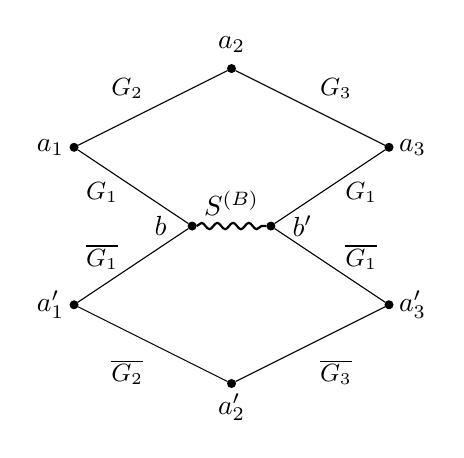
\begin{tikzpicture}[scale=1.0]

    % Define nodes with visible dots for origin
    \node[draw, circle, inner sep=1pt, fill=black] (A1) at (-2, 2) {};
    \node at (-2.3, 2) {$a_1$}; % Offset label above

    \node[draw, circle, inner sep=1pt, fill=black] (A2) at (0, 3) {};
    \node at (0 , 3.3) {$a_2$}; % Offset label to the right

    \node[draw, circle, inner sep=1pt, fill=black] (A3) at (2, 2) {};
    \node at (2.3, 2 ) {$a_3$}; % Offset label above

    \node[draw, circle, inner sep=1pt, fill=black] (B) at (-0.5, 1) {};
    \node at (-0.9, 1) {$b$}; % Offset label to the left

    \node[draw, circle, inner sep=1pt, fill=black] (B1) at (0.5, 1) {};
    \node at (0.9, 1) {$b'$}; % Offset label to the right

    \node[draw, circle, inner sep=1pt, fill=black] (A1b) at (-2, 0) {};
    \node at (-2.3, -0) {$a'_1$}; % Offset label below

    \node[draw, circle, inner sep=1pt, fill=black] (A2b) at (0, -1) {};
    \node at (0, -1.3) {$a'_2$}; % Offset label to the right

    \node[draw, circle, inner sep=1pt, fill=black] (A3b) at (2, 0) {};
    \node at (2.3, -0) {$a'_3$}; % Offset label below

    % Draw connections (upper diamond)
    \draw (A1) -- (A2) node[midway, above left] {\small $G_2$}; % Reduced font size
    \draw (A2) -- (A3) node[midway, above right] {\small $G_3$}; % Reduced font size
    \draw (A1) -- (B) node[midway, below left, xshift=-2pt, yshift= 5pt] {\small $G_1$}; % Adjusted position
    \draw (A3) -- (B1) node[midway, below right, xshift=2pt, yshift= 5pt] {\small $G_1$}; % Adjusted position

    % Draw connections (lower diamond)
    \draw (B) -- (A1b) node[midway, above left,  xshift=-2pt, yshift=-5pt] {\small $\overline{G_1}$}; % Reduced font size
    \draw (A1b) -- (A2b) node[midway, below left, yshift=-2pt] {\small $\overline{G_2}$}; % Adjusted position
    \draw (A2b) -- (A3b) node[midway, below right, yshift=-2pt] {\small $\overline{G_3}$}; % Adjusted position
    \draw (B1) -- (A3b) node[midway, above right, xshift=2pt, yshift=-5pt] {\small $\overline{G_1}$}; % Adjusted position

    % Connect b and b' with a wavy line and add "S" label
    \draw[decorate, decoration={snake, amplitude=0.4mm, segment length=2mm}, thick] (B) -- (B1)
        node[midway, above] {$S^{(B)}$};

    \end{tikzpicture}
   
\end{minipage}%
\hfill
\begin{minipage}{0.45\textwidth} % Adjust width as needed
    \raggedright
     % Adjust vertical alignment as needed
    $$k=1 $$\\ 
    $$\textbf{a}^{(1 )}=( a_1, a_2, a_3, b', a_3', a_2', a_1',b);$$
    \\  
     $$\boldsymbol{\sigma}^{(1 )}=(\;\sigma_1, \sigma_2, \sigma_3,\sigma_1, \overline{\sigma_1},\overline{\sigma_3}, \overline{\sigma_2},\overline{\sigma_1} ).$$
\end{minipage}
 \caption{Example of the $8-G$ loop in $\mathcal{E}\otimes  \mathcal{E}$: for $\sigma\in \{+,-\}^3$}
    \label{fig:8shapedgraph}
\end{figure}


\end{definition}

 

\begin{lemma}[The martingale term]\label{lem:DIfREP}
For any stopping time $T$ with respect to  $H_t$ and  $\tau:= t\wedge T$, we have  
 \begin{equation}\label{alu9_STime}
   \mathbb{E} \left| \int_{s}^\tau\left(\mathcal{U}_{u, t, \boldsymbol{\sigma}} \circ \mathcal{E}^{(M)}_{u, \boldsymbol{\sigma}}\right)_{\textbf{a}} \right|^{2p} 
   \le C_{n,p} \; 
   \mathbb{E} \left(\int_{s}^\tau 
   \left(\left(
   \mathcal{U}_{u, t,  \boldsymbol{\sigma}}
   \otimes 
   \mathcal{U}_{u, t,  \overline{\boldsymbol{\sigma}}}
   \right) \;\circ  \;
   \left( \mathcal{E} \otimes  \mathcal{E} \right)
   _{u, \,\boldsymbol{\sigma}  }
   \right)_{{\textbf a}, {\textbf a}}du 
   \right)^{p}
  \end{equation} 
  where  $\overline{\boldsymbol{\sigma}}$ is the conjugate sign vector of ${\boldsymbol{\sigma}}$. More precisely, as in \eqref{def_Ustz}, 
  $$
  \left[\left(
   \mathcal{U}_{u, t,  \boldsymbol{\sigma}}
   \otimes 
   \mathcal{U}_{u, t,  \overline{\boldsymbol{\sigma}}}
   \right)\circ \cal A\right]_{\textbf{a},\textbf{a}'}=
   \sum_{\textbf{b},\;\textbf{b}'} \; \prod_{i=1}^n \left(\frac{1 - u \cdot m_i m_{i+1} S^{(B)}}{1 - t \cdot m_i m_{i+1} S^{(B)}}\right)_{a_i b_i}
   \;\cdot \;\prod_{i=1}^n \left(\frac{1 - u \cdot \overline{m_i m_{i+1}} S^{(B)}}{1 - t \cdot \overline{m_i m_{i+1}} S^{(B)}}\right)_{a'_i b'_i} \cdot \mathcal{A}_{\textbf{b},\textbf{b}'}.
  $$
\end{lemma}
\begin{proof}[Proof of Lemma \ref{lem:DIfREP}]


 

We will prove the case $\tau =t$; the general case is identical. 
By Definition \ref{def_Edif}, $
 \mathcal{E}^{(M)}_{t, \boldsymbol{\sigma}, \textbf{a}}=\sum_{\alpha=(i,j)} \mathcal{E}^{(M)}_{t, \boldsymbol{\sigma}, \textbf{a}}(\alpha)\cdot d{\cal B}_\alpha(t) $ 
 and 
 $$
 \left(\mathcal{U}_{u, t, \boldsymbol{\sigma}}\circ \mathcal{E}^{(M)}_{u, \boldsymbol{\sigma}}\right)_{\textbf{a}}=
 \sum_{\alpha=(i,j)}
 \left(
 \mathcal{U}_{u, t, \boldsymbol{\sigma}} \circ\mathcal{E}^{(M)}_{u, \boldsymbol{\sigma}}
 (\alpha)
 \right)_{\textbf{a}}\cdot d{\cal B}_\alpha(u)
 $$
Here with $\quad \alpha=(i,j)$ we have 
$$
\mathcal{E}^{(M)}_{t, \boldsymbol{\sigma},\textbf{a}}
 (\alpha)
 =(S_{ij})^{1/2}\cdot \partial_{(H_t)_{ij}} {\cal L}_{t,\boldsymbol{\sigma},\textbf{a}}.
$$
Using  the chain rule and the structure of $\cal L$, we can write 
 $$
\mathcal{E}^{(M)}_{t, \boldsymbol{\sigma},\textbf{a}}
 (\alpha)=\sum_{k=1}^{n}\;\mathcal{E}^{(M)}_{t, \boldsymbol{\sigma},\textbf{a}}
 (\alpha, k), \quad \quad \mathcal{E}^{(M)}_{t, \boldsymbol{\sigma},\textbf{a}}
 (\alpha, k):=(S_{ij})^{1/2}\cdot  {\cal L}_{t,\boldsymbol{\sigma},\textbf{a}}\Big|\left(G_k\to \partial_{(H_t)_{ij}}G_k\right)$$
 where $(\alpha,k)$ denotes the term in which the derivative acts on the $k$-th $G$-edge of $\cal L$.  By definition  \eqref{defEOTE},  we have 
 $$
 \sum_\alpha   \mathcal{E}^{(M)}_{t, \boldsymbol{\sigma},\textbf{a}}
 (\alpha, k)\cdot \overline {\mathcal{E}^{(M)}_{t, \boldsymbol{\sigma},\textbf{a}'}(\alpha, k)}=
 \left(\mathcal{E}\otimes  \mathcal{E}\right)^{(k)}_{t, \,\boldsymbol{\sigma}, \,\textbf{a},\,\textbf{a}'}
 $$
 Since  $\cal U$ is a deterministic linear operator,   the  quadratic  variation of the martingale  term in \eqref{int_K-LcalE}
 can be bounded by 
 \begin{align} \label{UEUEdif}
  \left[\int \left(\mathcal{U}_{u, t, \boldsymbol{\sigma}} \circ \mathcal{E}^{(M)}_{u, \boldsymbol{\sigma}}\right)_{\textbf{a}} \right ]_t
\;=\; & \int_s^t
\sum_{\alpha}\left| \left(\mathcal{U}_{u, t, \boldsymbol{\sigma}} \circ\mathcal{E}^{(M)}_{u, \boldsymbol{\sigma}}(\alpha )\right)_{\textbf{a}}
 \right|^2 du 
 = \int_s^t
\sum_{\alpha}\left|\left(\sum_{k=1}^n \mathcal{U}_{u, t, \boldsymbol{\sigma}} \circ\mathcal{E}^{(M)}_{u, \boldsymbol{\sigma}}(\alpha, k)\right)_{\textbf{a}}
 \right|^2 du
 \nonumber \\
\; \;\le C_n\; &\int_s^t
\sum_{\alpha}\sum_{k=1}^n\left| \left(\mathcal{U}_{u, t, \boldsymbol{\sigma}} \circ\mathcal{E}^{(M)}_{u, \boldsymbol{\sigma}}(\alpha, k)\right)_{\textbf{a}}
 \right|^2 du
\nonumber \\
\;=\;C_n \; &\int_{s}^t
\left(\left(
   \mathcal{U}_{u, t,  \boldsymbol{\sigma}}
   \otimes 
   \mathcal{U}_{u, t,  \overline{\boldsymbol{\sigma}}}
   \right) \;\circ  \;
   \left( \mathcal{E} \otimes  \mathcal{E} \right)
   _{u, \,\boldsymbol{\sigma}  }
   \right)_{{\textbf a}, {\textbf a}} du.
\end{align}
Here we have used the Schwarz inequality in expanding the square. 
Our desired result,  \eqref{alu9_STime}, follows from the BDG inequality.
  
 
    
\end{proof}





 
  




\subsection{Proof of Theorem \ref{lem:main_ind}, step 2}
In this section,  we focus on the $(+,-)$ $2$-$G$-loop, i.e. $\boldsymbol{\sigma}=(+,-)$. The subscript $\boldsymbol{\sigma}$ will be dropped  in this subsection.  We will prove \eqref{Eq:Gdecay_w} first, and  \eqref{Gt_bound_flow} will be proved at the end of this  section. 
Define the tail functions ${\cal T}^{(\cal L-K)}_u (\ell)$ and ${\cal T}_{u,D} (\ell)$ 
\begin{equation}\label{def_WTu}
      {\cal T}^{(\cal L-K)}_u (\ell):= \max_{a,\,b\; : \; |a-b|\ge \ell} \left| ({\cal L-K})_{u,  \boldsymbol{\sigma},  ( a, b)}\right|,\quad  \boldsymbol{\sigma}=(+,-),
\end{equation}
\begin{equation}\label{def_WTuD}
{\cal T} _{u, D} (\ell) :=  (W\ell_u\eta_u)^{-2}
\exp \left(- \left( \ell /\ell_u \right)_+^{1/2} \right)+W^{-D}.
\end{equation} 
Both ${\cal T}^{(\cal L-K)}_u$ and ${\cal T}_{u,D}$ are non-increasing functions:
 $$
 0\le \ell_1\le \ell_2,\quad \quad 
 {\cal T}^{(\cal L-K)}_u (\ell_1)\ge {\cal T}^{(\cal L-K)}_u (\ell_2),\quad {\cal T} _{u,D} (\ell_1)\ge{\cal T} _{u,D}(\ell_2)
 $$
 Denote  the ratio between them by  % (the plus 1 is for the simplicity of future argument).
\begin{equation}\label{def_Ju}
     {\cal J} _{u,D} (\ell):=   \left({\cal T}^{(\cal L-K)}_u (\ell) \Big/{\cal T}_{u,D} (\ell)\right)+1
\end{equation} 
We aim to bound $ {\cal J} _{u,D} (\ell)$ for any $u\in [s,t]$ and large $D>0$, i.e., 
 \begin{align}\label{shoellJJ}
    {\cal J}^* _{u,D} :=\max_{\ell}   {\cal J} _{u,D} (\ell)\le (\eta_s/\eta_u)^4 
  \end{align}
Define a  scale parameter 
$$
  \ell^{*}_t := (\log W)^{3/2}\cdot \ell_t .
$$
In this scale $\ell_t^*$,  $\Theta_t$ is exponentially small, whereas ${\cal T}_t$ is not. 
More precisely, we have the following lemma.  
\begin{lemma}\label{lem_dec_calE_0}
For any fixed large $D$ and small $\delta>0$,  
 \begin{align}
 \label{Kell*}
   |b -a|\ge \delta \cdot \ell_t^* &\implies 
   \left({\Theta}_t\right)_{ab } \le W^{-D} ,\quad    \left({\Theta}_s^{-1}{\Theta}_t\right)_{ab } \le W^{-D}
   \\
  |b -a|\ge \delta \cdot \ell_t^* 
 & \implies  {\cal L}_{t, (-,+),(a, b)} \prec {\cal J}^*_{t,D}\cdot{\cal T}_{t,D}(|a-b|) . \label{auiwii}
\end{align}
For any constant $C>0$, \begin{equation}\label{Tell*}
       { {\cal T}_{u,D} \left(\ell-C\cdot \ell_u^*\right)}\;\prec \;  {\cal T}_{u,D} \left(\ell \right).
\end{equation} 

\end{lemma}
\begin{proof} We will only prove \eqref{auiwii}. By definition, 

\[
{\cal L}_{t, (-,+),(a, b)} = \left({\cal L} - \cal K\right)_{t, (-,+),(a, b)} + {\cal K}_{t, (-,+),(a, b)}.
\]
Using the $\Theta$ representation of the 2-\(\cal K\) in \eqref{Kn2sol} and the decay property of \(\Theta\) from \eqref{prop:ThfadC}, we have  for any \(D > 0\) that 
\[
{\cal K}_{t, (-,+),(a, b)} \prec N^{-D} \leq {\cal T}_{t, D}(|a-b|).
\]
Together with the definition \eqref{shoellJJ}  of \(\cal J^*\), \eqref{def_Ju}, and \eqref{def_WTu}, we have proved  \eqref{auiwii}.
We remark that \eqref{auiwii} is significant because ${\cal T}_{t,D}$ is smaller by a factor of
$(W\eta_t\ell_t)^{-1}$ than the typical size of a 2-${\cal L}$ loop. The extra small factor comes from the assumption $|b-a|\ge \delta\ell_t^*$.
\end{proof} 

Our proof of \eqref{Eq:Gdecay_w}   relies on the loop hierarchy \eqref{int_K-L_ST} in the special case $n=2$. 
We begin the analysis of the hierarchy by  bounding  terms in \eqref{int_K-L_ST}.  

\begin{lemma}\label{lem_dec_calE}  Suppose  the assumptions of Theorem  \ref{lem:main_ind} and the conclusions  of Step 1, i.e., \eqref{lRB1} and \eqref{Gtmwc}, 
hold. Assume that 
\begin{align} 
s\le u\le t, \quad  D\ge 10, \; \textbf{a}=(a_1,a_2),\; \textbf{a}'=(a'_1,a'_2),\; \boldsymbol{\sigma}=(+,-), \quad 
\max_i |a_i-a_i'|\le \ell_t ^*. \label{57}
\end{align}
 We  have 
\begin{align}\label{res_deccalE_lk}
       {\cal E}^{( (L-K)\times(L-K) )}
       _{u, \boldsymbol{\sigma},\textbf{a}} \Big/\; 
  {\cal T}_{t,D}(|a_1-a_2|) \quad 
 \;  &\; \prec \; 
   \left(\eta_u\right)^{-1} 
   \cdot  
   \left(W\eta_u\ell_u\right)^{-1}
    \cdot 
 \left({\cal J}^{*}_{u,D} \right)^{2}
 \\
      \mathcal{E}^{( \widetilde{G} )}_{u, \boldsymbol{\sigma},\textbf{a}} 
    \;\Big/\; 
 {\cal T}_{t,D}(|a_1-a_2|)
 \;  &\; \prec \; 
 \left(\eta_u\right)^{-1} 
  \cdot \left(\ell_u/\ell_s\right)^2\cdot{\bf 1}(|a_1-a_2|\le \ell_u^*)
    \nonumber  \\
       \;  &\; + \;  \left(\eta_u\right)^{-1} 
  \cdot
       \left(W \eta_u \ell_u\right)^{-3/7}  \cdot 
       \left({\cal J}^{*}_{u,D} \right)^{3}
 \label{res_deccalE_wG}\\
\label{res_deccalE_dif}
    \left(
   \mathcal{E}\otimes  \mathcal{E} \right)
   _{u, \,\boldsymbol{\sigma},  \,{\textbf a} ,\, {\textbf a}'
     }
     \;\Big/\; 
 \left( {\cal T}_{t,D}(|a_1-a_2|)\right)^2
 \;  &\; \prec \; 
  \left(\eta_u\right)^{-1} 
  \cdot \left(\ell_u/\ell_s\right)^5\cdot{\bf 1}(|a_1-a_2|\le 4\ell_t^*)
     \nonumber \\
       \;  &\; + \;  \left(\eta_u\right)^{-1} \cdot \left(\ell_u/\ell_s\right)^{3/2} 
  \cdot
       \left(W \eta_u \ell_u\right)^{-1/2}  \cdot 
    \left({\cal J}^{*}_{u,D} \right)^{3}
\end{align} 
  \end{lemma}
By assumption  \eqref{con_st_ind},  $s$ and $t$ are near each other.  So the exact exponents  on the right side  of \eqref{res_deccalE_lk}-\eqref{res_deccalE_dif} are not important for our purpose.  We only need the errors to be of the form 
$$
  (\eta_s/\eta_t)^\alpha\cdot \left(W \eta_u \ell_u\right)^{-\beta}\cdot \left({\cal J}^{*}_{u,D} \right) ^{\gamma}
  $$
for some positive constants $\alpha$, $\beta$ and $\gamma$. 

We now provide a power counting to guess the sizes of terms in the previous lemma. Since 
$ {\cal E}^{( (L-K)\times(L-K) )}$ is a higher order term, we will ignore it in the following heuristic. 
Denote by $A_u \sim  W\ell_u\eta_u$. By definition, $\mathcal{E}^{( \widetilde{G} )}_u$ is a product of a $1$-$\cal L-\cal K$ loop and 
a $3$-$\cal L$ loop. We know that  $1$-$\cal L -\cal K$ loop is of order $A_u^{-1}$ and $3$-$\cal L$ loop is of order $A_u^{-2}$. In addition, 
the  summation index in $\mathcal{E}^{( \widetilde{G} )}$ yields a factor $\ell_u$ if we assume the correct decay property. Since there is an additional $W$ factor in $\mathcal{E}^{( \widetilde{G} )}_u$, 
\begin{align}
\mathcal{E}^{( \widetilde{G} )}_u \sim A_u^{-3} W \ell_u = \eta_u^{-1} A_u^{-2}.
\end{align}
The factor $A_u^{-2}$ is exactly the prefactor  in the definition of $ {\cal T}_u$ in \eqref{res_deccalE_wG}.  For $ \mathcal{E}\otimes  \mathcal{E}_u $, it is a $6$-$\cal L$ loop of order $A_u^{-5}$. Hence 
\begin{align}
(\mathcal{E}\otimes  \mathcal{E})_u \sim A_u^{-5} W \ell_u = \eta_u^{-1} A_u^{-4}, 
\end{align}
which explains the order in \eqref{res_deccalE_dif}.  Notice that in both \eqref{res_deccalE_wG} and  \eqref{res_deccalE_dif}, 
we used $ {\cal T}_t$ on the left sides of the equations while both $\mathcal{E}^{( \widetilde{G} )}_u$ and $(\mathcal{E}\otimes  \mathcal{E})_u$ are at the time $u$. 

So far we only used the loop bounds which are consequences of Step 1. 
It remains to understand the last terms in \eqref{res_deccalE_wG} and  \eqref{res_deccalE_dif}. Assuming  Lemma \ref{lem_dec_calE}, we now  prove  \eqref{Eq:Gdecay_w}. We will use extensively the kernel estimates concerning  the operator $\cal U$ in Section \ref{ks}. 


\begin{proof}[Proof of \eqref{Eq:Gdecay_w}]
By  assumption \eqref{Eq:Gdecay+IND} on $({ \cal L-\cal K})_s$, the operator norm bound on $\cal U$ in Lemma \ref{lem:sum_Ndecay},  and the  tail estimate  \eqref{neiwuj}, 
%of Lemma \ref{TailtoTail}, 
we can  bound the first term on the right side  of \eqref{int_K-L_ST} by 
\begin{equation} \label{res_deccalE_0}
\left(\mathcal{U}_{s, t, \boldsymbol{\sigma}} \circ (\mathcal{L} - \mathcal{K})_{s, \boldsymbol{\sigma}}\right)_{\textbf{a}}\;\Big/\; 
  {\cal T}_{t, D}(|a_1-a_2|) \quad 
  \prec \;   (\ell_t/\ell_s)^2\cdot {\bf 1}(|a_1-a_2|\le \ell_t^*) + 1,
\end{equation}
where the last term of order one comes from applying \eqref{neiwuj}. Notice that the expansion factor $\left(\eta_u / \eta_t\right)^2$  from applying Lemma \ref{lem:sum_Ndecay} has become 
$ (\ell_t/\ell_s)^2$ due to the prefactors in $ {\cal T}_{s, D}$ and  ${\cal T}_{t, D}$.
For  any $\textbf{a}$ fixed and any function $f$,  we decompose $f  = f_1  + f_2   $ where 
$f_1 (\textbf{b}) = f (\textbf{b}) {\bf 1} ( \| \textbf{b}-\textbf{a}\|\le \ell_t^*) $. 
From the decay of ${\cal U}_{u,t}$,  $\Big ( {\cal U}_{u,t, \boldsymbol{\sigma}} \circ f_2 \Big)_\textbf{a}$ is exponentially small.  
Hence we only have to bound $  {\cal U}_{u,t, \boldsymbol{\sigma}} \circ f_1$, for which we apply  Lemma \ref{lem:sum_Ndecay}. Therefore,  
we can bound the second  term of \eqref{int_K-L_ST} by 
$$
 \Big({\cal U}_{u,t, \boldsymbol{\sigma}}\circ  {\cal E}^{( (L-K)\times(L-K) )}_{u, \boldsymbol{\sigma}}\Big)_\textbf{a}
 \prec (\eta_u/\eta_t)^2 \max_{\| \textbf{b}-\textbf{a}\|\le \ell_t^*}{\cal E}^{( (L-K)\times(L-K) )}_{u, \boldsymbol{\sigma}, \textbf{b}}+W^{-D}, 
$$
$$
 \|\textbf{b}-\textbf{a}\|=\max_i |b_i-a_i|\le \ell_t^*.
 $$
Under the last  condition, \eqref{Tell*} implies that 
$$
 {\cal T}_{t, D}(|b_1-b_2|)\prec  {\cal T}_{t, D}(|a_1-a_2|).
$$
Using the estimate \eqref{res_deccalE_lk} for ${\cal E}^{((L-K)\times(L-K))}$ and the $(s,t)$-condition \eqref{con_st_ind}, we have 
\begin{align} 
\label{res_deccalE_1}
     \Big({\cal U}_{u,t, \boldsymbol{\sigma}}\circ  {\cal E}^{( (L-K)\times(L-K) )}_{u, \boldsymbol{\sigma}}\Big)_\textbf{a}\;\Big/\; 
 {\cal T}_{t, D}(|a_1-a_2|) \quad 
  & \prec \; 
  \frac{1}{\eta_u}\left(\eta_u / \eta_t\right)^2 
   \cdot  
   \left(W\eta_u\ell_u\right)^{-1 }
    \cdot 
\left({\cal J}^*_{u,D}\right)^2
\end{align} 
Similarly,   the estimate \eqref{res_deccalE_wG} on ${\cal E}^{(\widetilde{G} )}$ implies   
\begin{align}  \label{res_deccalE_2}
     \Big(\mathcal{U}_{u,t, \boldsymbol{\sigma}} \circ  \mathcal{E}^{( \widetilde{G} )}_{u, \boldsymbol{\sigma}}\Big)_{\mathbf{a}} 
    \;\Big/\; 
{\cal T}_{t, D}(|a_1-a_2|)
 &\prec \;  {\bf1}(|a_1-a_2|\le 3\ell_t^*)\cdot  \frac{1} {\eta_u} \cdot \left(\eta_u / \eta_t\right)^2\cdot \left(\ell_u / \ell_s\right)^2 
 \nonumber \\
  &+\;    \frac{1}{\eta_u} 
  \cdot\left(\eta_u / \eta_t\right)^2 \cdot
       \left(W \eta_u \ell_u\right)^{-3/7}  \cdot \left({\cal J}^{*}_{u,D} \right)^{3 }, 
       \end{align} 
and  the  estimate  \eqref{res_deccalE_dif} on $\cal E\otimes\cal E$  implies  
\begin{align} \label{res_deccalE_3}
  \left(\left(
   \mathcal{U}_{u, t,  \boldsymbol{\sigma}}
   \otimes 
   \mathcal{U}_{u, t,  \overline{\boldsymbol{\sigma}}}
   \right) \;\circ  \;
   \left( \mathcal{E} \otimes  \mathcal{E} \right)
   _{u, \,\boldsymbol{\sigma}  }
   \right)_{{\textbf a}, {\textbf a}}
     \;\Big/\; 
 \left({\cal T}_{t, D}(|a_1-a_2|)\right)^2
 &\prec \;  {\bf1}(|a_1-a_2|\le 6\ell_t^*)\cdot  \frac{1} {\eta_u} \cdot \left(\eta_u / \eta_t\right)^4\cdot \left(\ell_u / \ell_s\right)^5 
 \nonumber \\
 &+ \;  \frac{1}{\eta_u} 
  \cdot
       \left(W \eta_u \ell_u\right)^{-1/3}  \cdot \left({\cal J}^{*}_{u,D} \right)^{3 }  
\end{align}
In the last inequality, we have absorbed the  expansion factor $\left(\eta_u / \eta_t\right)^4$ by the change of the exponent in $   \left(W \eta_u \ell_u\right)$ from $-1/2$ to $-1/3$.  


We now insert  these bounds   into the $2$-$G$-loop equation \eqref{int_K-L_ST} and 
bound  the martingale term by \eqref{alu9_STime}.
Denote by $T$ the stopping time 
\begin{align}
T:=\min \{u: {\cal J}^*_{u,D} \ge N^{\delta}\left(\eta_s / \eta_t\right)^4\}
\end{align}
where $\delta>0$ is fixed and arbitrarily small, and set $\tau = T \wedge t$. 
Clearly, the stopped versions of Lemma \ref{lem_dec_calE} and the previous bounds in this proof are valid by similar arguments. 
The quadratic variation of the stopped  martingale term is then bounded by 
\begin{align}\label{51}
& \int_s^\tau  \left( \left(\mathcal{U}_{u,t,  \boldsymbol{\sigma}}
   \otimes 
   \mathcal{U}_{u, t,  \overline{\boldsymbol{\sigma}}}
   \right) \;\circ  \;
   \left( \mathcal{E} \otimes  \mathcal{E}  \right)
   _{u, \,\boldsymbol{\sigma},\, \overline{\boldsymbol{\sigma}} }
   \right)_{{\textbf a}, {\textbf a}}  d u
 \Big/{\cal T}_{t, D}(|a_1-a_2|)^2  \nonumber \\
 \;\prec \; &   \int_s^\tau   d u \Big \{ 
 {\bf1}(|a_1-a_2|
\le 6\ell_t^*)\cdot  \frac{1} {\eta_u} \cdot \left(\eta_u / \eta_t\right)^4\cdot \left(\ell_u / \ell_s\right)^5 
+ \;  \frac{1}{\eta_u} 
  \cdot
       \left(W \eta_u \ell_u\right)^{-1/3}  \cdot \left({\cal J}^{*}_{u,D} \right)^{3 }  \Big \}   \nonumber \\
\;\prec \; &    \big [ (\eta_s/\eta_t)^{4}(\ell_t/\ell_s)^{5}  \cdot {\bf 1}(|a_1-a_2|\le 6\ell_t^*)+(\eta_s/\eta_t)^{3} \big ].
 \end{align}
Applying  \eqref{alu9_STime}, we have 
 $$
 \int_s^\tau\left(\mathcal{U}_{u, t, \sigma} \circ \mathcal{E}_{u, \sigma}^{(M)}\right)_{\textbf{a}}\;\Big/{\cal T}_{t, D}(|a_1-a_2|)
 \prec \big [ (\eta_s/\eta_t)^{2}(\ell_t/\ell_s)^{5/2}  \cdot {\bf 1}(|a_1-a_2|\le 6\ell_t^*)+(\eta_s/\eta_t)^{3/2} \big ].
 $$
 This statement holds for any $t\ge s$. Furthermore, due to the monotonicity of $\ell$ and $\eta$, for any $s\le t'\le t$ we have
\begin{align}\label{bsluwous1}
  \int_s^{T\wedge t'}\left(\mathcal{U}_{u,t', \sigma} \circ \mathcal{E}_{u, \sigma}^{(M)}\right)_{\textbf{a}}\;\Big/{\cal T}_{t', D}(|a_1-a_2|)
   & \; \prec \; \big [ (\eta_s/\eta_{t'})^{2}(\ell_{t'}/\ell_s)^{5/2}  \cdot {\bf 1}(|a_1-a_2|\le 6\ell_{t'}^*)+(\eta_s/\eta_{t'})^{3/2} \big ]
 \\\nonumber
  & \; \prec \;  \big [ (\eta_s/\eta_{t })^{2}(\ell_{t }/\ell_s)^{5/2}  \cdot {\bf 1}(|a_1-a_2|\le 6\ell_{t }^*)+(\eta_s/\eta_{t })^{3/2} \big ]
 \end{align}
 We extend this bound to a $N^{-C}$ net between $s$ and $t$, i.e., $t^{(k)}=s+(t-s)\cdot k\cdot N^{-C}$   for a fixed large $C$.  
 \begin{align}\label{bsluwous2}
  & \max_k\int_s^{T\wedge t^{(k)}} \left(\mathcal{U}_{u,\, t^{(k)},\, \sigma} \circ \mathcal{E}_{u, \sigma}^{(M)}\right)_{\textbf{a}}\;\Big/{\cal T}_{t^{(k)}, \,D}(|a_1-a_2|) \prec  \big [ (\eta_s/\eta_{t })^{2}(\ell_{t }/\ell_s)^{5/2}  \cdot {\bf 1}(|a_1-a_2|\le 6\ell_{t }^*)+(\eta_s/\eta_{t })^{3/2} \big ]
 \end{align}
For any $k$, we can rewrite  the last term in   \eqref{int_K-L_ST} as follows: 
%equals the following term.  
$$
 %t^{(k)}\ge \tau=T\wedge t\; \implies \;  
 {\cal U}_{t,\tau}\circ \int_{s}^\tau \left(\mathcal{U}_{u, t, \boldsymbol{\sigma}} \circ \mathcal{E}^{(M)}_{u, \boldsymbol{\sigma}}\right)_{\textbf{a}}\;=\;{\cal U}_{t^{(k)},\tau }\int_s^{\tau } \left(\mathcal{U}_{u,\, t^{(k)},\, \sigma} \circ \mathcal{E}_{u, \sigma}^{(M)}\right)_{\textbf{a}} 
$$
Choose  a $k$ such that  $t^{(k-1)}\le \tau < t^{(k)}$. Then $T\wedge t^{(k)}= \tau$. 
Since $C$ can be chosen arbitrarily large,  $ {\cal U}_{t^{(k)},\tau }$ is  nearly an identity operator. Then
$$
{\cal U}_{t^{(k)},\tau }\int_s^{\tau } \left(\mathcal{U}_{u,\, t^{(k)},\, \sigma} \circ \mathcal{E}_{u, \sigma}^{(M)}\right)_{\textbf{a}} =\int_s^{\tau } \left(\mathcal{U}_{u,\, t^{(k)},\, \sigma} \circ \mathcal{E}_{u, \sigma}^{(M)}\right)_{\textbf{a}} +O(N^{-C/2})
$$
and
$$
{\cal T}_{t^{(k)}, \,D}(|a_1-a_2|)\Big/{\cal T}_{\tau, \,D}(|a_1-a_2|)=1+O(N^{-C/2})
$$
Combining  these two bounds, we have 
$$
 {\cal U}_{t,\tau}\circ \int_{s}^\tau \left(\mathcal{U}_{u, t, \boldsymbol{\sigma}} \circ \mathcal{E}^{(M)}_{u, \boldsymbol{\sigma}}\right)_{\textbf{a}} \; \Big/\; {\cal T}_{\tau, \,D}(|a_1-a_2|) \prec  \big [ (\eta_s/\eta_{t })^{2}(\ell_{t }/\ell_s)^{5/2}  \cdot {\bf 1}(|a_1-a_2|\le 6\ell_{t }^*)+(\eta_s/\eta_{t })^{3/2} \big ]
 $$
 Combining this  bound with  \eqref{res_deccalE_0}, \eqref{res_deccalE_1},   \eqref{res_deccalE_2}  and  \eqref{int_K-L_ST}, we have 
$$
\left({\cal L}-{\cal K}\right)_{\tau, \textbf{a}}\Big/{\cal T}_{t, D}(|a_1-a_2|) \prec   \big [ (\eta_s/\eta_t)^{2}(\ell_t/\ell_s)^{5/2}  \cdot {\bf 1}(|a_1-a_2|\le 6\ell_t^*)+(\eta_s/\eta_t)^{3/2} \big ], 
$$
where we have used the initial condition ${\cal J}^*_{s,D} \prec 1$ from \eqref{Eq:L-KGt+IND} and \eqref{Eq:Gdecay+IND}.  


 
This implies that 
\begin{align}\label{52}
 {\cal J}^*_{\tau,D}\prec     (\eta_s/\eta_t)^{2}(\ell_t/\ell_s)^{5/2}+(\eta_s/\eta_t)^{3/2}  
\end{align}
Since $\ell_t/\ell_s\le(\eta_s/\eta_t)^{1/2}$ and $\eta_s/\eta_t\ge 1$, the right side of \eqref{52} is at most $2(\eta_s/\eta_t)^{13/4} < N^{\delta}(\eta_s/\eta_t)^4$. Hence  ${\mathbb P} (T\le t )\le N^{-D}$ and we have completed  the proof of \eqref{Eq:Gdecay_w}.
We remark that integrating the near-field drift jointly in time yields the stronger bound ${\cal J}^*_{\tau,D}\prec(\eta_s/\eta_t)^{2}$.
 Notice that we have also proved 
\begin{align}\label{53}
\left({\cal L}-{\cal K}\right)_{t, \textbf{a}}\Big/{\cal T}_{t, D}(|a_1-a_2|) \prec   \big [ (\eta_s/\eta_t)^{2}(\ell_t/\ell_s)^{5/2}  \cdot {\bf 1}(|a_1-a_2|\le 6\ell_t^*)+(\eta_s/\eta_t)^{3/2} \big ].
\end{align}

\smallskip
\noindent\emph{The region $|a_1-a_2|>6\ell^*_t$.} The far-field prefactor $(\eta_s/\eta_t)^{3/2}$ in \eqref{53} is not bounded; we remove it by a second pass. Applying \eqref{52} with $t$ replaced by any $u\in[s,t]$ and using $\ell_u/\ell_s\le(\eta_s/\eta_u)^{1/2}$, we have ${\cal J}^*_{u,D}\prec(\eta_s/\eta_u)^{13/4}$ uniformly in $u\in[s,t]$. Fix $v\in[s,t]$ and write $r:=\eta_s/\eta_v$ and $A:=W\ell_v\eta_v$, so that $r^{30}\le A$ by \eqref{con_st_ind}. We insert this bound once more into \eqref{res_deccalE_0}--\eqref{res_deccalE_3}, with $t$ replaced by $v$, using $\eta_s/\eta_u\le r$ and $W\ell_u\eta_u\ge A$ for $u\le v$, and we localize the martingale term at the stopping time $T':=\min\{u:{\cal J}^*_{u,D}\ge N^{\delta'}r^{13/4}\}$ for a fixed small $\delta'>0$; ${\mathbb P}(T'\le v)$ is negligible by the first pass. For $|a_1-a_2|>6\ell^*_v$ all terms containing an indicator function vanish. Relative to ${\cal T}_{v,D}(|a_1-a_2|)$, and up to the factor $\int_s^v\eta_u^{-1}du=O(\log N)$, the remaining terms are bounded by $r^{17/2}A^{-1}\le A^{-43/60}$ (from \eqref{res_deccalE_1}), $r^{47/4}A^{-3/7}\le A^{-31/840}$ (from \eqref{res_deccalE_2}) and, for the quadratic variation, $r^{39/4}A^{-1/3}\le A^{-1/120}$ (from \eqref{res_deccalE_3}), so that the martingale term is $\prec A^{-1/240}$; the far part of \eqref{res_deccalE_0} is $\prec 1$. Since $A\ge W\ell_t\eta_t\ge N^{c}$ for some $c>0$ (by $t\le 1-N^{-1+\tau}$), these negative powers of $A$ absorb the factors $N^{\varepsilon}$. Hence
\begin{equation*}
\big({\cal L}-{\cal K}\big)_{v, \textbf{a}}\Big/{\cal T}_{v, D}(|a_1-a_2|) \prec 1,\qquad |a_1-a_2|>6\ell_v^*,
\end{equation*}
uniformly in $v\in[s,t]$.

    
\end{proof}
 

 \begin{proof}[Proof of Lemma \ref{lem_dec_calE}]
\emph{Proof of \eqref{res_deccalE_lk}.}  
We first  note the monotonicity properties 
$$
u\le t\implies \ell_u\le \ell_t,   \quad {\cal T}_{u,D}\le {\cal T}_{t,D} .$$
By definition, 
\begin{align} {\cal E}^{( ({\cal L-K})\times({\cal L-K}) )}_{u,  \boldsymbol{\sigma},  \textbf{a} }
= &W\sum_{b_1,b_2}({\cal L-K})_{u,
\boldsymbol{\sigma}, 
( a_1, b_1)
}
S^{(B)}_{b_1,b_2}
({\cal L-K})_{u,  \boldsymbol{\sigma},  ( b_2, a_2)}
\end{align}
By definition of $S^{(B)}$,  we have $|b_1-b_2|\le 1$.  
Using 
$$
\int_{0 }^a\exp\left(-\sqrt{(a-x)}-\sqrt x+ \sqrt a\right)dx\le C\approx 6.12
,\quad \text{ and } \quad 
\int_{0 }^\infty\exp\left({-\sqrt x}\right)dx=2
$$
we have 
\begin{align}\nonumber
{\cal E}^{( ({\cal L-K})\times({\cal L-K}) )}_{u,  \boldsymbol{\sigma},  \textbf{a} }
\; \prec \;& W ({\cal J}_{u,D}^*) ^2\cdot 
\sum_{x }  {\cal T}_{u, \,D}(|a_1-x|) \cdot {\cal T}_{u, \,D}(|a_2-x|)   
\\\label{mmxiaoxi}
\; \prec \;&
({\cal J}_{u,D}^*) ^2 \cdot 
 \eta_u^{-1}\cdot (W\ell_u\eta_u)^{-1}\cdot  {\cal T}_{u,D }(|a_1-a_2|) .
\end{align} 
We  have thus proved   \eqref{res_deccalE_lk}.

 
\medskip
\noindent 
\emph{Proof of   \eqref{res_deccalE_wG}}.    By definition, we  write 
\begin{align}
 \max_{\textbf{a}}{\cal E}^{(\widetilde G)}_{u,  \boldsymbol{\sigma},  \textbf{a} }
 \prec W \sum_{b_1,b_2} \langle \widetilde G_u E_{b_1}\rangle\cdot S^{(B)}_{b_1,b_2}\cdot  {\cal L}_{u, (-,+,+),(a_2, b_2, a_1)}+c.c.,\quad \widetilde{G}=G-m
 \end{align}
By \eqref{GavLGEX} and \eqref{Gtmwc}, we have 
$$
\langle \widetilde G_u E_{b_1}\rangle\prec \Xi^{(\cal L)}_{u,2}\cdot (W\ell_u\eta_u)^{-1}\prec  (W\ell_u\eta_u)^{-1}+ {\cal J}^*_{u,D}\cdot (W\ell_u\eta_u)^{-2}.
$$
Therefore 
 \begin{align}\label{jiizziy}
\max_{\textbf{a}}{\cal E}^{(\widetilde G)}_{u,  \boldsymbol{\sigma},  \textbf{a} } \prec \frac{1}{ \ell_u\eta_u} \cdot \sum_{b }   \left|{\cal L}_{u, (-,+,+),(a_1, b , a_2)}\right|(1+{\cal J}^*_{u,D}(W\ell_u\eta_u)^{-1})
\end{align}
Consider first the case  $|a_1-a_2|\le \ell_u^*$.  Denote 
$$
\ell_u^{**}:= \ell_u\cdot (\log W)^3=\ell^*_u\cdot (\log W)^{3/2}
$$
Clearly,  ${\cal T}_{u,D}(\ell_u^{**})\prec W^{-D}$. 
For $|b-a_1|\le  \ell_u^{**}$, 
the loop bound \eqref{lRB1}  proved in the Step 1 implies that 
\begin{align}\label{alkkj}
 \sum_{b }{\bf 1}\big(|b-a_1|\le  \ell_u^{** }\big)\cdot  \left|{\cal L}_{u, (-,+,+),(a_1, b , a_2)}\right|\prec (\ell_u/\ell_s)^2\cdot (W\ell_u\eta_u)^{-2} \cdot \ell_u   
\end{align}
where the summation over $b$ provides a factor $ \ell_u^{** } \prec\ell_u$. 
If $|b-a_1|\ge \ell_u^{**}$, we can easily bound 
 $$
 \left|{\cal L}_{u, (-,+,+),(a_1, b , a_2)}\right|\prec \max_{x_1\in {\cal I}_{a_1},y\in {\cal I}_{b}}|G_{x_1,y}|.
$$
Using  \eqref{GijGEX}, we have that 
$$
\max_{x_1\in {\cal I}_{a_1},y\in {\cal I}_{b}}|G_{x_1,y}|\prec \sum_{a_1', b'}\left({\cal L}_{u,(+,-),{(a_1',b')}}\right)^{1/2}{\bf1}\left(|a'_1-a_1|\le 1, |b-b'|\le 1\right).
$$
Since $|b-a_1|\ge \ell_u^{** }$, by  \eqref{auiwii} and ${\cal T}_{u,D}(|a_1-b|)\prec W^{-D}$, we obtain that  
$$
{\cal L}_{u,(+,-),{(a_1',b')}} \prec {\cal J}^*_{u,D}\cdot W^{-D}.
$$
Therefore, the contribution from $|b-a_1|\ge  \ell_u^{** }$ part is negligible in the sense 
\begin{align}\label{alkkj2}
 \sum_{b }{\bf 1}\big(|b-a_1|\ge  \ell_u^{** }\big)\cdot  \left|{\cal L}_{u, (-,+,+),(a_1, b , a_2)}\right|\prec  {\cal J}^*_{u,D}\cdot W^{-10}. 
\end{align}
It  is easy to check that the contribution of the last term does not affect the argument given below.  Furthermore,  the contributions from both  \eqref{alkkj} and  \eqref{jiizziy} are bounded by 
\begin{align}\label{82jjdopasj}
 |a_1-a_2|\le \ell_u^*\implies  \mathcal{E}_{u, \boldsymbol{\sigma}, \mathbf{a}}^{(\widetilde{G})} \Big/{\cal T}_{u,D}(|a_1-a_2|)\prec 
 (\eta_u)^{-1} \cdot \left(\ell_u / \ell_s\right)^2\cdot   \left(1+  (\mathcal{J}_{u, D}^*)^2 \left(W \ell_u \eta_u\right)^{-1 }\right).
 \end{align}
This implies that   \eqref{res_deccalE_wG} holds for $|a_1-a_2|\le \ell_u^*$. Here the term $(\eta_u)^{-1}(\ell_u/\ell_s)^2({\cal J}^*_{u,D})^2(W\ell_u\eta_u)^{-1}$ of \eqref{82jjdopasj} is bounded by the second term of \eqref{res_deccalE_wG}, since ${\cal J}^*_{u,D}\ge 1$ and $(\ell_u/\ell_s)^2\le \eta_s/\eta_u\le (W\ell_u\eta_u)^{1/30}$ by \eqref{con_st_ind}.



For   $|a_1-a_2|\ge \ell_u^*$,  we split it into  two cases  
 $$
 (1): \min_i|a_i-b|\le \ell_u^*/2,\quad \quad 
 (2): \min_i|a_i-b|\ge \ell_u^*/2.
 $$
In the first case,  we assume without loss of generality that $|a_1-b|\le \ell_u^*/2$. Applying  the Schwarz inequality to  the two $G$ edges  in ${\cal L}_{u, (-,+,+),(a_1, b , a_2)}$ connecting the block $a_2$,  we have 
$$
G_{x_1x_2}G_{x_2y}G_{yx_1}\prec |G_{x_1x_2}|^2|G_{yx_1}|+
|G_{ x_2 y}|^2|G_{yx_1}|.
$$
Therefore, we have 
\begin{align}\label{kskjw}
  {\cal L}_{u, (-,+,+),(a_1, b , a_2)}
  \;\prec\; &\;  W^{-1} \Big ( {\cal L}_{u, (-,+),(a_1, a_2)} \ \max_{x_1\in {\cal I}_{a_1}}\sum_{y\in {\cal I}_{b}}|G_{x_1y}|+ {\cal L}_{u, (-,+),(a_2, b)}\ \max_{y\in {\cal I}_{b}}\sum_{x_1\in {\cal I}_{a_1}}|G_{x_1y}| \Big )  .
\end{align}
Using \eqref{GijGEX},  the $\cal K$ bound and the trivial fact $\sqrt { 1+c } \le 1+c $,  we can bound $|G_{x_1x_2}|$ by 
$$
{\bf 1}(x_1\ne x_2)|G_{x_1x_2}|\prec (W\ell_u\eta_u)^{-1/2}(1+{\cal J}^*_{u,D}(W\ell_u\eta_u)^{-1}).
$$
It implies that for any $a $ and $b$, 
\begin{align}\label{jaysw2002}
  W^{-1}  \max_{y\in{\cal I}_b}\sum_{x\in{\cal I}_a}|G_{xy}|\prec (W\ell_u\eta_u)^{-1/2}(1+{\cal J}^*_{u,D}(W\ell_u\eta_u)^{-1}).
\end{align}
Inserting  this bound  into \eqref{kskjw}, we have 
\begin{align}
  {\cal L}_{u, (-,+,+),(a_1, b , a_2)}
     \;\prec\; &\;\left( {\cal L}_{u, (-,+),(a_1, a_2)}   + {\cal L}_{u, (-,+),(a_2, b)}  \right)  \cdot (W\ell_u\eta_u)^{-1/2}(1+{\cal J}^*_{u,D}(W\ell_u\eta_u)^{-1})
\end{align}
 Since $|a_2-b|\ge \ell_u^*/2$ and $|a_1-a_2|\ge  \ell_u^*$,  we can estimate  $ {\cal L}_{u, (-,+),(a_1, a_2)}   + {\cal L}_{u, (-,+),(a_2, b)}$ 
with \eqref{auiwii} to have  
$$
 {\cal L}_{u, (-,+,+),(a_1, b , a_2)} \;\prec\; {\cal J}^*_{u,D}\cdot \left(  {\cal T}_{u,D}(|a_1-a_2|)+{\cal T}_{u,D}(|b-a_2|) \right)  \cdot (W\ell_u\eta_u)^{-1/2}(1+{\cal J}^*_{u,D}(W\ell_u\eta_u)^{-1}).
 $$
Furthermore since $|b-a_2|\ge |a_1-a_2|-|a_1-b|\ge |a_1-a_2|-\ell_u^*/2$, then
$${\cal T}_{u,D}(|b-a_2|) \prec  {\cal T}_{u,D}(|a_1-a_2|).
$$
Combining these bounds,  we obtain,   for $|a_1-a_2|\ge \ell_u^*$, that  
\begin{align}
    \label{lwjufw}
    \sum_{b } ^{\text{Case } 1} \left|{\cal L}_{u, (-,+,+),(a_1, b , a_2)}\right|\prec \left({\cal J}^*_{u,D}\right)^2\cdot{\cal T}_{u,D}(|a_1-a_2|) \cdot \ell_u(W\ell_u\eta_u)^{-1/2} .
\end{align}
For case (2),  we bound  ${\cal L}_{u, (-,+,+),(a_1, b , a_2)}$ as follows
\begin{align}\label{LGGGXXX}
{\cal L}_{u, (-,+,+),(a_1, b , a_2)}
\prec \max_{x_1,x_2, y} \left|G_{x_1y}\right| \left|G_{yx_2}\right|\left|G_{x_1x_2}\right|{\bf 1}(x_1\in {\cal I}_{a_1}){\bf 1}(x_2\in {\cal I}_{a_2}){\bf 1}(y\in {\cal I}_{b}).
\end{align}
 In this case, since $a_1$, $a_2$ and $b$ are all different,  $x_1$, $x_2$ and $y$ must be different.  
 
 
 Next we use   \eqref{GijGEX} to bound a single $G$ with the $2$-$G$-loops.   Because $a_1$, $a_2$ and $b$ are away from each other by $\ell_u^*/2$, we have, by  \eqref{auiwii}, 
 \begin{align}\label{GGTLJ}
 \left|G_{yx_2}\right|\cdot \left|G_{x_1x_2}\right| \cdot
\left|G_{x_1y}\right|
\;\prec \; & \left({\cal J}^*_{u,D}\right)^{3/2} \Big( {\cal T}_{u,D}(|a_1-a_2|) {\cal T}_{u,D}(|a_1-b|){\cal T}_{u,D}(|a_2-b|)\Big)^{1/2}
 \end{align}
Then we can bound 
\begin{align}
    \sum_{b}^{ \text {Case } 2 }{\cal L}_{u, (-,+,+),(a_1, b , a_2)} 
 \;\prec \;  &\;\left({\cal J}^*_{u,D}\right)^{3/2}\Big( {\cal T}_{u,D}(|a_1-a_2|)\Big)^{1/2} \sum_b \Big({\cal T}_{u,D}(|a_1-b|){\cal T}_{u,D}(|a_2-b|)\Big)^{1/2}
 \nonumber \\
  \;\prec \; &\;\left({\cal J}^*_{u,D}\right)^{3/2}\Big( {\cal T}_{u,D}(|a_1-a_2|)\Big) \cdot  \ell_u\cdot  (W\ell_u\eta_u)^{-1}
\end{align}
where we have used
$$
\int_{0 }^a\exp\left(-\sqrt{(a-x)}/2-\sqrt x/2+ \sqrt a/2\right)dx\le C .
$$
Combining  this estimate with \eqref{lwjufw}, we obtain that if $|a_1-a_2|\ge \ell_u^*$ then
\begin{align}
    \sum_{b} {\cal L}_{u, (-,+,+),(a_1, b , a_2)} 
  \;\prec \; &\;\left({\cal J}^*_{u,D}\right)^2\Big( {\cal T}_{u,D}(|a_1-a_2|)\Big) \cdot  \ell_u\cdot  (W\ell_u\eta_u)^{-1/2}
\end{align}
Inserting  it into \eqref{jiizziy} and using  \eqref{82jjdopasj}, we have completed the proof of  \eqref{res_deccalE_wG}.

 \medskip
\emph{Proof of \eqref{res_deccalE_dif}. } By definition \eqref{defEOTE},  $(\mathcal{E} \otimes \mathcal{E})$ is the sum of  $(\mathcal{E} \otimes \mathcal{E})^{(k)}$, and the latter ones can be written in terms of the following loops $
{\cal L}^{(k )}:= {\cal L}_{u, \boldsymbol{\sigma}^{(k ) },\textbf{a}^{(k )}} $. Here
$ \boldsymbol{\sigma}^{(1 )}=( +,-,+,-,+,-)$, $\textbf{a}^{(1 )}=( a_1,a_2, b', a_2',a_1',b)$
and $\boldsymbol{\sigma}^{( 2)}= $ $(-,+,-,+,-,+)$, $\textbf{a}^{( 2)}=( a_2,a_1, b', a_1',a_2',b)$. Hence  by symmetry, we only need to prove \eqref{res_deccalE_dif} for $(\mathcal{E} \otimes \mathcal{E})^{(1)}$, i.e.,  $k=1$ case. Notice that $|b-b'| = 1$ in this case and 
we can treat $b=b'$ for all practical purposes in the following proof. 
 
\begin{figure}[ht]
\centering
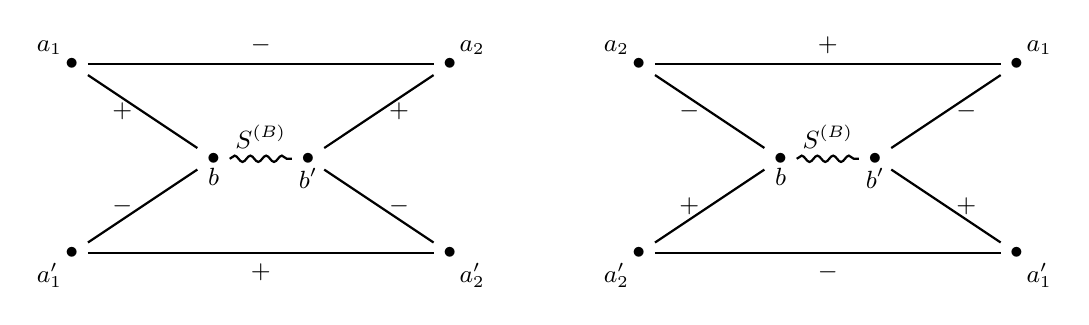
\begin{tikzpicture}[scale=1.2, every node/.style={font=\small}]

% Left graph
\node (a1) at (0, 2) {$\bullet$};
\node[above left] at (a1) {$a_1$};

\node (a2) at (4, 2) {$\bullet$};
\node[above right] at (a2) {$a_2$};

\node (b) at (1.5, 1) {$\bullet$};
\node[below] at (b) {$b$};

\node (b') at (2.5, 1) {$\bullet$};
\node[below] at (b') {$b'$};

\node (a1') at (0, 0) {$\bullet$};
\node[below left] at (a1') {$a_1'$};

\node (a2') at (4, 0) {$\bullet$};
\node[below right] at (a2') {$a_2'$};

\draw[thick] (a1) -- (b) node[midway, left] {$+$};
 \draw[thick] (b') -- (a2) node[midway, right] {$+$};
\draw[thick] (b') -- (a2') node[midway, right] {$-$};
 \draw[thick] (b) -- (a1') node[midway, left] {$-$};
\draw[thick] (a1) -- (a2) node[midway, above] {$-$};
\draw[thick] (a1') -- (a2') node[midway, below] {$+$};
\draw[decorate, decoration={snake, amplitude=0.4mm, segment length=2mm}, thick] (b) -- (b')
        node[midway, above] {$S^{(B)}$};

% Right graph
\node (a1r) at (6, 2) {$\bullet$};
\node[above left] at (a1r) {$a_2$};

\node (a2r) at (10, 2) {$\bullet$};
\node[above right] at (a2r) {$a_1$};

\node (br) at (7.5, 1) {$\bullet$};
\node[below] at (br) {$b$};

\node (b'r) at (8.5, 1) {$\bullet$};
\node[below] at (b'r) {$b'$};

\node (a1r') at (6, 0) {$\bullet$};
\node[below left] at (a1r') {$a_2'$};

\node (a2r') at (10, 0) {$\bullet$};
\node[below right] at (a2r') {$a_1'$};

\draw[thick] (a1r) -- (br) node[midway, left] {$-$};
 \draw[thick] (b'r) -- (a2r) node[midway, right] {$-$};
\draw[thick] (b'r) -- (a2r') node[midway, right] {$+$};
 \draw[thick] (br) -- (a1r') node[midway, left] {$+$};
\draw[thick] (a1r) -- (a2r) node[midway, above] {$+$};
\draw[thick] (a1r') -- (a2r') node[midway, below] {$-$};
\draw[decorate, decoration={snake, amplitude=0.4mm, segment length=2mm}, thick] (br) -- (b'r)
        node[midway, above] {$S^{(B)}$};
        
\end{tikzpicture}
\caption{\hspace{.1in} Left: $k=1$; \hspace{1.4in} right: $k=2$.}
\label{fig:graph-6Gfor2G}
\end{figure}

\noindent 
{\bf Case 1: $|a_1-a_2|\le 4\ell_t^*$ } 
%First   prove \eqref{res_deccalE_dif}  for $(\mathcal{E} \otimes \mathcal{E})^{(1)}$ in the case  $|a_1-a_2|\le 4\ell_t^*$.  
We split the sum $\sum_{b,b'}$ into two parts 
$$
|b-a_1|\le \ell_u^{** }:=(\log W)^3 \ell_u,\quad |b-a_1|\ge \ell_u^{** } 
$$
Using ${\cal T}_{u,D}(\ell_u^{** }) $ is very small,  one can easily bound 
$$
\sum_{b,b'} {\bf 1}\left(|b-a_1|\ge \ell_u^{** }\right){\cal L}^{(1)}\prec {\cal J}^*_{u,D}\cdot W^{-3},
$$
by arguments similar to those used in \eqref{alkkj2}.
For $|b-a_1|\le  \ell_u^{** } $, we use 
the loop bound \eqref{lRB1} proved in Step 1 to have 
\begin{align}\label{alkkj3}
\sum_{b,b'}{\bf 1}\big(|b-a_1|\le  \ell_u^{** }\big) {\cal L}^{(1)}  \prec (\ell_u/\ell_s)^5\cdot (W\ell_u\eta_u)^{-5} \cdot \ell_u   .
\end{align}
Combining  these two bounds, we obtain that \eqref{res_deccalE_dif} holds for $|a_1-a_2|\le 4\ell_t^*$. Notice that the application of the loop bound of length $6$ yields a very strong bound $(W\ell_u\eta_u)^{-5}$ which is not easy to see without the loop estimate. 

 \medskip


 \noindent 
{\bf Case 2: $|a_1-a_2|\ge 4\ell_t^*$ .} 
% Recall  $|a'_i-a_i|\le \ell_t^*, \quad a_1-a_2\ge 4\ell_t^*$.
Recall  the assumption  $|a'_i-a_i|\le \ell_t^*$ \eqref{57} and the fact  that we can treat $b=b'$  in the following proof.  
We  split the sum over $b$ (and $b'$) into two parts 
$$
(1): |b -a_1|\le |b-a_2|,\quad (2): |b-a_1|\ge |b-a_2|.
$$
By symmetry (exchanging $a_1\leftrightarrow a_2$ and cutting the loop at $b'$ instead of $b$), we only consider  the first case.   Similar to \eqref{LGGGXXX} (see also figure \ref{fig:graph-6Gfor2G}), we  bound ${\cal L}^{(1)}$ by the product of four $G$'s and  $G^\dagger E_b G$ as follows: 
\begin{align} 
{\cal L}^{(1)}\le W^{-2}   \max_{ x_2\in {\cal I}_{a _2}}\max_{ y'\in {\cal I}_{b'}}\max_{x_2'\in {\cal I}_{a'_2}} \sum_{x_1\in {\cal I}_{a_1}}\sum_{x'_1\in {\cal I}_{a'_1}}
\left|G_{x_1x_2}\right|
\left|G_{x_2y'}\right|
\left|G_{y'x_2'}\right|
\left|G_{ x_2'x_1'}\right|
\left|\left(G^\dagger E_b G\right)_{ x_1x_1'}\right|.
\end{align}
Using the Cauchy--Schwarz inequality (on $\sum_{x_1,x'_1}$) and the definition $\cal L$, we have
\begin{align}\label{L6G6X}
{\cal L}^{(1)}\le \max^*_{x_1,x_2,y',x_1',x_2'}  
\left|G_{x_1x_2}\right|
\left|G_{x_2y'}\right|
\left|G_{y'x_2'}\right|
\left|G_{ x_2'x_1'}\right|
\cdot \left(\max_{ \textbf{a}}\max_{\boldsymbol{\sigma}\in \{+,-\}^4 }{\cal L}_{u,\boldsymbol{\sigma},\textbf{a}}\right)^{1/2}, 
\end{align}
where the $\max $ is over  the condition 
$$
 {\bf 1}(x_1\in {\cal I}_{a_1}){\bf 1}(x_2\in {\cal I}_{a_2}){\bf 1}(y'\in {\cal I}_{b'}){\bf 1}(x'_1\in {\cal I}_{a'_1}){\bf 1}(x'_2\in {\cal I}_{a'_2}).
$$
We claim that 
\begin{align} \label{GGTLJ4G}
|G_{y'x_2}|\cdot |G_{y'x_2'}| 
\cdot 
|G_{x_1x_2}|\cdot |G_{x_1'x_2'}|
\prec 
\left({\cal J}^*_{u,D}\right)^2\cdot 
{\cal T} _{t,D}(|a_1-a_2|)\cdot {\cal T} _{t,D}( |b-a_2|)  .  
\end{align}
To prove this bound, we split it into two cases:  
\begin{align}
(1a): \;&\; |a_1-b|\le \ell_u^*,\quad \text{or}\quad |a_1'-b|\le \ell_u^*\nonumber \\
(1b):   \;&\;  |a_1-b|\ge \ell_u^*,\quad and\quad |a_1'-b|\ge \ell_u^*.
\end{align} 
Since $|a_1-a_2|\ge 4\ell_t^*$, we have,  similar to \eqref{GGTLJ}, that 
\begin{align} 
 |G_{x_1x_2}|^2\prec  & {\cal J}^*_{u,D}\cdot {\cal T}_{u,D}(|a_1-a_2|), \\
 |G_{x_1'x_2'}|^2\prec & {\cal J}^*_{u,D}\cdot {\cal T}_{u,D}\left( |a_1'-a_2'|\right)  \prec {\cal J}^*_{u,D}\cdot {\cal T}_{t,D}\left( |a_1-a_2|\right), 
\end{align} 
where  we have used ${\cal T}_u\le {\cal T}_t$, the assumption $|a_i'-a_i|\le \ell_t^*$ and \eqref{Tell*} in the   second inequality.  Thus we have 
$$
|G_{x_1x_2}|\cdot |G_{x_1'x_2'}|\prec   {\cal J}^*_{u,D}\cdot {\cal T}_{t,D}\left( |a_1-a_2|\right).
$$ 
For edges connecting with $b'$, we have 
$$
|G_{y'x_2}|\cdot |G_{y'x_2'}| \prec 
{\cal J}^*_{u,D}\cdot  {\cal T}^{1/2}_{u,D}\left( |b-a_2| \right)\cdot   {\cal T}^{1/2}_{u,D}\left(  |b-a_2'| \right),
$$
where we have used that  both  $|b-a_2|$ and $|b-a_2'|$ are larger than $\ell_t^*\ge \ell_u^*$.
Using  ${\cal T}_u\le {\cal T}_t$ and $|a_2-a_2'|\le \ell_t^*$, we have 
$$
|G_{y'x_2}|\cdot |G_{y'x_2'}|\prec {\cal J}^*_{u,D}\cdot  {\cal T} _{t,D}\left(  |b-a_2| \right).
$$
Combining  these  bounds, we have proved \eqref{GGTLJ4G}. 

Next, applying  \eqref{lRB1} on $\cal L$ term in \eqref{L6G6X}, together with \eqref{GGTLJ4G} we obtain that 
$$
{\cal L}^{(1)}\prec (\ell_u/\ell_s)^{3/2}\left(W\ell_u\eta_u\right)^{-3/2}\cdot \left({\cal J}^*_{u,D}\right)^2\cdot 
{\cal T} _{t,D}(|a_1-a_2|)\cdot {\cal T} _{t,D}( |b-a_2|)  . 
$$
Consider the case (1a) so that   $|a_2-b|\ge |a_1-a_2|-\ell_t^*$. Therefore, ${\cal T} _{t,D}\left(  |b-a_2| \right) \prec 
{\cal T} _{t,D}\left(  |a_1-a_2| \right)$. 
Combining  these bounds  with \eqref{GGTLJ4G}, we have 
\begin{align}
  \sum_{b,b'}^{(1a)} {\cal L}^{(1)}
 \prec &(\ell_u/\ell_s)^{3/2} \cdot \ell_u \cdot\left(W \ell_u \eta_u\right)^{-3/2}
\cdot\left({\cal J}^*_{u,D}\right)^2  \cdot \left({\cal T}_{t,D}(|a_1-a_2|)\right)^2.
\end{align}
For (1b), we bound  $(G^\dagger E_bG)_{x_1x_1'}$ by 
$$
(G^\dagger E_bG)_{x_1x_1'}\le \max_{y\in {\cal I}_b}|G_{yx_1}||G_{yx'_1}|.
$$
Since  $ |a_1-b|,\; |a_1'-b| \ge \ell_u^*$,    we have, similar to \eqref{GGTLJ}, 
$$
(G^\dagger E_bG)_{x_1x_1'}
\prec {\cal J}^*_{u,D} \cdot  {\cal T}_{t,D}(|b-a_1|) .
$$
Together  with \eqref{GGTLJ4G}, we have  
\begin{align}
  \sum_{b,b'}^{(1b)} {\cal L}^{(1)}
 \prec\; & \left( {\cal J}^*_{u,D}\right)^3 \cdot  {\cal T}_{t,D}(|a_1-a_2|)\cdot \sum_b {\cal T}_{t,D}(|b-a_1|) {\cal T}_{t,D}(|b-a_2|)
 \nonumber \\
\prec \; &  \left( {\cal J}^*_{u,D}\right)^3 \cdot \ell_t \cdot (W\ell_t\eta_t)^{-2} 
\cdot \left({\cal T}_{t,D}(|a_1-a_2|)\right)^{2}.
 \end{align}
Here the last line was bounded as in the proof of \eqref{mmxiaoxi}.  Putting  the bounds for (1a) and (1b) together, we obtain \eqref{res_deccalE_dif} and complete the proof of Lemma  \ref{lem_dec_calE}. 
\end{proof}

 

\noindent 
\begin{proof}[Proof of \eqref{Gt_bound_flow}] Combining  the $\cal L-\cal K$ estimate  \eqref{Eq:Gdecay_w} and the $\cal K$ bound in Lemma \ref{ML:Kbound}, we obtain that
\begin{equation}
\label{lk2safyas}
 \max_{a, b}{\cal L }_{u, (+,-), (a,b)}\prec \left(\eta_s/\eta_u\right)^4\cdot (W\ell_u\eta_u)^{-2}+(W\ell_u\eta_u)^{-1}\prec (W\ell_u\eta_u)^{-1}  ,\quad u\in [s,t]    
\end{equation}
where we have used the induction hypothesis  \eqref{con_st_ind}. 
Then we can apply  the resolvent entry estimate in Lemma \ref{lem_GbEXP}.  The weak local law in \eqref{Gtmwc} implies the assumptions of  Lemma \ref{lem_GbEXP}. From \eqref{GiiGEX}, \eqref{GijGEX} and  \eqref{lk2safyas}, we have 
$$
\|G_u-m\|^2_{\max}\prec  \max_{a, b}{\cal L }_{u, (+,-), (a,b)}\prec (W\ell_u\eta_u)^{-1} .
$$
This completes the proof of \eqref{Gt_bound_flow}.   
\end{proof}

  
\subsection{Fast decay property}
In the second step of the proof for Theorem \ref{lem:main_ind}, we established the decay property of the $2\text{-}G$ loop in \eqref{Eq:Gdecay_w}. In this subsection, we extend this decay property to general loops $\mathcal{L}$ and $\mathcal{L} - \mathcal{K}$. This decay property is highly useful for bounding the $\mathcal{E}$ terms in equation \eqref{int_K-LcalE}. We begin by defining the $\ell_u$-decay property.


\begin{definition}[The decay property]\label{Def_decay}
   Let  $\cal A$ be a tensor $\mathbb Z_L^n\to \mathbb R$. We say $\cal A$ has $(u, \tau, D)$ decay at the  time $u$ if  for some fixed small $\tau>0$ and large $D>0$, we have  
\begin{equation}\label{deccA}
    \max_{1\le i,j\le n}\|a_i-a_j\|\ge \ell_u W^{\tau} \implies  {\cal A}_{\textbf{a}}=O(W^{-D}),\quad \textbf{a}=(a_1,a_2,\ldots,a_n) .
\end{equation}
\end{definition}
\begin{lemma}[The decay property of ${\cal L}_u$]\label{lem_decayLoop}  
Assume that \eqref{Gt_bound_flow} and \eqref{Eq:Gdecay_w} hold. Then  for 
any $n\ge 2$, any small $\tau$, large $D$ and $D'>0$,  the  ${\cal L}_u$ has $(u, \tau, D)$ decay  with probability $1-O(W^{-D'})$. More precisely, 
\begin{align}\label{res_decayLK}
\mathbb P\left( \max_{\boldsymbol{\sigma},\,\textbf{a}}  \Big(\left|{\cal L}_{u,\boldsymbol{\sigma},\textbf{a}}\right|+\left|({\cal L}-{\cal K})_{u,\boldsymbol{\sigma},\textbf{a}}\right|\Big)\cdot{\bf 1}\left(\max_{  i, j } \|a_i-a_j\|\ge \ell_u W^{\tau}\right) \ge W^{-D}\right)\le W^{-D'} .
\end{align}
 \end{lemma}
 \begin{proof}[Proof of Lemma \ref{lem_decayLoop}] Combining  the decay properties  of ${\cal K}_{u,(+,-)}$ and $\cal L-\cal K$  \eqref{Eq:Gdecay_w}, we obtain that  
 ${\cal L}_{u,(+,-)}$ has $(u, \tau, D)$ decay property  for any fixed $(\tau, D)$  with high probability.
 Applying the $G_{ij}$ estimate in \eqref{GijGEX} and  the new ${\cal L}_u$ decay property, we have 
 $$
   \forall \tau, D, D', \quad \mathbb P\left( \max_{i\in {\cal I}_{a_1}}\max_{j\in {\cal I}_{a_2}}|G_{ij}|
 \cdot{\bf 1}\left( |a_1-a_2|\ge \ell_u W^{\tau}\right) \ge W^{-D}\right)\le W^{-D'} .
 $$
By definition  ${\cal L}=\langle \prod\limits_{i=1}^n \bigl(G_iE_{a_i}\bigr)\rangle $  has the $(u, \tau, D)$ decay property.  On the other hand, by the decay of $\Theta^{(B)}_t$ and  the tree representation of $\cal K$ in Lemma \ref{eq_trcalK},  $\cal K$ also   has $(u, \tau, D)$ decay property. Therefore $({\cal L-\cal K})_u$ has $(u, \tau, D)$ decay property. 
 
 \end{proof}


The evolution kernel satisfies a straightforward $L_\infty \to L_\infty$ bound, stated as a bound on $\|{\cal U}_{u,t}\|_{\max\to \max}$ in Lemma \ref{lem:sum_Ndecay}.
When the tensor acted on by ${\cal U}_{u,t}$ is short-ranged and satisfies a sum-zero property, Lemma \ref{lem:sum_decay} gives a substantial improvement.
These two estimates yield the following bounds on the $\cal E$ terms.


%The decay property enables us to use  Lemma \ref{lem:sum_decay} for $\|{\cal U}_{u,t}\|_{\max\to \max}$ on fast decay tensors. This provides a major  improvement over using Lemma \ref{lem:sum_Ndecay} to bound $\|{\cal U}_{u,t}\|_{\max\to \max}$.  




 \begin{lemma}[Bounds on $\cal E$ terms] \label{lem_BcalE} 
Assume  that \eqref{Gt_bound_flow} and \eqref{Eq:Gdecay_w} hold.  
Define $\Xi^{({\cal L})}$ and  $\Xi^{({\cal L}-{\cal K})}$ as follows
\begin{align}\label{def:XIL-K}
  \Xi^{({\cal L} )}_{t, m} &:= \max_{\boldsymbol{\sigma}, \textbf{a}} \left|{\cal L} _{t, \boldsymbol{\sigma}, \textbf{a}} \right|\cdot \left(W\ell_t \eta_t\right)^{m-1} \cdot {\bf 1}(\boldsymbol{\sigma} \in \{+, -\}^m),  
\\\nonumber
     \Xi^{({\cal L}-{\cal K})}_{t, m} &:= \max_{\boldsymbol{\sigma}, \textbf{a}} \left|({\cal L}-{\cal K})_{t, \boldsymbol{\sigma}, \textbf{a}} \right|\cdot \left(W\ell_t \eta_t\right)^{m} \cdot {\bf 1}(\boldsymbol{\sigma} \in \{+, -\}^m).
\end{align}
Then 
\begin{align}\label{CalEbwXi}
\big[\mathcal{K} \sim(\mathcal{L}-\mathcal{K})\big]_{u, \boldsymbol{\sigma}}^{l_{\mathcal{K}}}
   \; \prec \; &
   \left( \max_{k<n }\Xi^{(\cal L-\cal K)}_{u,k}\right)\cdot (W\ell_u\eta_u)^{-n }\cdot \frac{1}{\eta_u}  , 
   \nonumber \\
    \mathcal{E}_{u, \boldsymbol{\sigma}}^{((\mathcal{L} - \mathcal{K}) \times (\mathcal{L} - \mathcal{K}))}
    \; \prec \; &
   \left( \max_{k:\;2\le k\le n }\Xi^{(\cal L-\cal K)}_{u,k}\cdot \Xi^{(\cal L-\cal K)}_{u,n-k+2}\cdot(W\ell_u\eta_u)^{-1}\right)\cdot (W\ell_u\eta_u)^{-n }\cdot \frac{1}{\eta_u}  , 
  \nonumber \\  \mathcal{E}_{u, \boldsymbol{\sigma}}^{(\widetilde{G})}
 \; \prec \; &
     \Xi^{(\cal L)}_{u,n+1} \cdot (W\ell_u\eta_u)^{-n }\cdot \frac{1}{\eta_u}   ,  
  \nonumber \\   
(\mathcal{E} \otimes \mathcal{E}) _{u, \boldsymbol{\sigma}}
\; \prec \; &  \; \Xi^{(\cal L)}_{u, {2n+2}}\cdot   (W\ell_u\eta_u)^{-2n } \cdot \frac1{\eta_u}. 
\end{align}
Furthermore, 
all these  $\cal E$ terms have the $(u, \tau, D)$ decay property for  $u\in [s,t]$.  
 \end{lemma}
 
 \begin{proof}[Proof of Lemma \ref{lem_BcalE}] The proof  follows directly from the definitions of these  terms  %and the  $\cal E$ terms, 
 and the decay properties in Lemma \ref{lem_decayLoop}.  
     \begin{itemize}
    \item By definition \eqref{DefKsimLK},  $\mathcal{K} \sim(\mathcal{L}-\mathcal{K})$ can be written as the product of $\cal K$  and $\cal L-\cal K$ loops.   Bounding  $\cal K$  with \eqref{eq:bcal_k}, we have  
    \begin{align}
    \big[\mathcal{K} \sim(\mathcal{L}-\mathcal{K})\big]_{u, \boldsymbol{\sigma}}^{l_{\mathcal{K}}}
 \; \prec \; &
 W\cdot (W\ell_u\eta_u)^{-l_{\mathcal{K}}+1}\cdot \ell_u\cdot \Xi^{(\cal L-\cal K)}_{u,(n-l_{\mathcal{K}}+2)}\cdot (W\ell_u\eta_u)^{-(n-l_{\mathcal{K}}+2)}
    \end{align}
    where we used $l_{\mathcal{K}}\ge 3$ and the $\ell_u$ factor comes from the sum of the index $a$, which was restricted by the decay property of $\mathcal K$. 
    As a side remark, the other index  $b$ was restricted by    $S^{(B)}_{ab}$. 
    
    \item By  definition \eqref{def_ELKLK},  $ \mathcal{E}^{((\mathcal{L} - \mathcal{K}) \times (\mathcal{L} - \mathcal{K}))}$ can be written as the product of two loops, whose total length is $n+2$.
    \begin{align}
   \mathcal{E}^{((\mathcal{L} - \mathcal{K}) \times (\mathcal{L} - \mathcal{K}))}
 \; \prec \; &
 W\cdot \sum_{k=2}^{n} \Xi^{(\cal L-\cal K)}_{u, \,k}
 \cdot (W\ell_u\eta_u)^{-k}
 \cdot \ell_u\cdot \Xi^{(\cal L-\cal K)}_{u,(n-k+2)}
 \cdot (W\ell_u\eta_u)^{-(n-k+2)}
      \end{align}
    
    \item By definition \eqref{def_EwtG}, 
    $\mathcal{E}^{(\widetilde{G})}$  can be written as the product of  a  $(\cal L-\cal K)$ loop of length one and an  $(n+1)-G$  loop. With  \eqref{GavLGEX}, we have 
    \begin{align}
  \mathcal{E}^{(\widetilde{G})}
 \; \prec \; &
 W\cdot   \max_{a,b}{\cal L}_{u,(+,-),(a,b)}
 \cdot \ell_u\cdot \Xi^{\cal L }_{u,(n+1)}
 \cdot (W\ell_u\eta_u)^{-n} 
    \end{align} 
    Furthermore, by \eqref{Eq:Gdecay_w}, Lemma \ref{ML:Kbound} and \eqref{con_st_ind} (see \eqref{lk2safyas}), we have $\max_{a,b}{\cal L}_{u,(+,-),(a,b)}\prec (W\ell_u\eta_u)^{-1}$. 
 \item By definition  \eqref{def_diffakn_k}, 
    $(\mathcal{E} \otimes \mathcal{E})$ can be written in terms of  $(2n+2)$-$G$-loops.  Thus 
    \begin{align}
(\mathcal{E} \otimes \mathcal{E}) \prec  \Xi^{(\cal L)}_{u, {2n+2}}\cdot  W\cdot\ell_u\cdot (W\ell_u\eta_u)^{-2n-1 } .
    \end{align} 
\end{itemize}
Here all  $\ell_u$ factors  come from summing an index restricted to a range $\ell_u$. 
 \end{proof}
  
In the remainder of this subsection, we will use %hese estimates in 
Lemma \ref{lem_BcalE} to  improve estimates on $\cal L-\cal K$.  

\begin{lemma}\label{lem:STOeq_NQ} 
Assume that $\boldsymbol{\sigma}$ is not an alternating sign vector, i.e., 
\begin{equation}\label{NALsigm}
    \exists k,\; s.t.\; \sigma_k=\sigma_{k+1}.
\end{equation} 
Suppose that the   assumptions of  Theorem \ref{lem:main_ind},  the local law \eqref{Gt_bound_flow} and the decay property for $\cal L-\cal K$ \eqref{Eq:Gdecay_w} hold. If 
 $$
 \max_{u\in [s,t]}\, \Xi^{(\cal L)}_{u, {2n+2}}\prec {  \Lambda}
 $$
 for some deterministic quantity $ \Lambda \ge 1$, 
then 
\begin{align}\label{am;asoiuw}
 \Xi^{({\cal L-\cal K})}_{u,n}
 \;\prec\;  &\; { \Lambda}^{1/2}+\max_{u\in [s,t]}
  \left(\; \max_{k<n }\Xi^{({\cal L-\cal K})}_{u,k}+\max_{k:\;2\le k\le n }\Xi^{({\cal L-\cal K})}_{u,k}\cdot \Xi^{({\cal L-\cal K})}_{u,n-k+2}\cdot(W\ell_u\eta_u)^{-1}+\Xi^{({\cal L})}_{u,n+1}\right).
\end{align}
 
 
\end{lemma}

\begin{proof}[Proof of Lemma \ref{lem:STOeq_NQ}]
 By  case 1 of \eqref{sum_res_2}, %for fast decay tensors satisfying \eqref{NALsigm},  
$$
\big\|{\cal U}_{u,t,\boldsymbol{\sigma}}\big\|_{\max\to \max}\Big|({\rm fast\; decay \;tensor satisfying \eqref{NALsigm}})\le C_n W^{C_n \tau} \cdot\left(\frac{\ell_u \eta_u}{\ell_t \eta_t}\right)^n.
$$
 By  assumptions of  
 Theorem \ref{lem:main_ind} on  $({\cal L-K})_{s}$, the $\cal E$ estimates in Lemma \ref{lem_BcalE}, and   the previous bound on  $\max\to \max$ norm of ${\cal U}_{u,t}$, 
 we have 
\begin{align}\label{sahwNQ}
  (W\ell_t\eta_t)^n\cdot      (\mathcal{L} - \mathcal{K})_{t, \boldsymbol{\sigma}, \textbf{a}} \;\prec\; \; &
  1+   \int_{s}^t  \left( \max_{k<n }\Xi^{({\cal L-\cal K})}_{u,k}\right) \cdot \frac{1}{\eta_u}   du 
    \nonumber \\
    &+ \int_{s}^t \left( \max_{k:\;2\le k\le n }\Xi^{({\cal L-\cal K})}_{u,k}\cdot \Xi^{({\cal L-\cal K})}_{u,n-k+2}\cdot(W\ell_u\eta_u)^{-1}\right)\cdot \frac{1}{\eta_u} du 
    \nonumber \\
    &+ \int_{s}^t \Xi^{(\cal L)}_{u,n+1}\cdot \frac1{\eta_u} du 
   +
   (W\ell_t\eta_t)^n\cdot\int_{s}^t \left(\mathcal{U}_{u, t, \boldsymbol{\sigma}} \circ    \mathcal{E}^{(M)}_{u, \boldsymbol{\sigma}}\right)_{\textbf{a}} du. 
\end{align}
By Lemma \ref{lem:DIfREP},  we know that 
\begin{equation} \label{sahwNQ2}
   \mathbb{E} \left [    \int_{s}^t \left(\mathcal{U}_{u, t, \boldsymbol{\sigma}} \circ \mathcal{E}^{(M)}_{u, \boldsymbol{\sigma}}\right)_{\textbf{a}} \right ]^{2p} 
   \le C_{n,p} \; 
   \mathbb{E}    \left(\int_{s}^t 
   \left(\left(
   \mathcal{U}_{u, t,  \boldsymbol{\sigma}}
   \otimes 
   \mathcal{U}_{u, t,  \overline{\boldsymbol{\sigma}}}
   \right) \;\circ  \;
   \left( \mathcal{E} \otimes  \mathcal{E} \right)
   _{u, \,\boldsymbol{\sigma}  }
   \right)_{{\textbf a}, {\textbf a}}du 
   \right)^{p}.
\end{equation} 
Using  \eqref{CalEbwXi} to bound $\mathcal{E} \otimes  \mathcal{E}$, we have 
\begin{align}\label{sahwNQ3}
   (W\ell_t\eta_t)^{2n}\cdot  \int_{s}^t  \left(\mathcal{U}_{u, t, (\boldsymbol{\sigma}, \overline{\boldsymbol{\sigma}})} \;\circ  \;
   \left( \mathcal{E} \otimes  \mathcal{E} \right)
   _{u, \,\boldsymbol{\sigma}  }
   \right)_{{\textbf a}, {\textbf a}}du
   \prec \int_{s}^t \Xi^{(\cal L)}_{u, {2n+2}}\cdot \frac{1}{\eta_u}du . 
\end{align}
This completes the proof of Lemma \ref{lem:STOeq_NQ}. 
 
\end{proof}






 

\subsection{Sum zero operator \texorpdfstring{${\cal Q}_t$}{Qt}}
In this subsection, we introduce another key tool, ${\cal Q}_t$,  for estimating the loop hierarchy. 
\begin{definition}[Definition of ${\cal Q}_t$]\label{Def:QtPt} Let ${\cal A}_\textbf{a}$ be a tensor with $\textbf{a}\in\mathbb Z_L^n$, $n\ge 2$.   Define ${\cal P}$  by
$$
\left( {\cal P} \circ {\cal A}\right)_{a_1}= \sum_{a_2,\, a_3\cdots a_n}  {\cal A}_{\textbf{a}} ,\quad \textbf{a}=(a_1,\cdots,a_n), 
$$
where the index $a_1$ was fixed. A tensor $A$ has a sum zero property if and only if $ {\cal P} \circ {\cal A}= 0$.   Define 
$$
 \left({\cal Q}_t\circ {\cal A}\right)_{\textbf{a}}={\cal A}_{\textbf{a}}-\left({\cal P} \circ {\cal A}\right)_{a_1}
 \cdot {  \vartheta}_{t,\,\textbf{a}},\quad 
 {  \vartheta}_{t, \textbf{a}}:=\big(1-t\big)^{n-1}\prod_{i=2}^n \left(\Theta^{(B)}_t\right)_{a_1a_i}.
$$
Since $\sum_b\left(\Theta^{(B)}_t\right)_{ab}=(1-t)^{-1}$, it is easy to check that $ {\cal P} \circ  \vartheta_{t,\textbf{a}}=1$ 
and  ${\cal P} \circ {\cal Q}_t =0$. 
\end{definition}
The reason for using $\vartheta_{t,\textbf{a}}$ in the definition of ${\cal Q}_t$ is to preserve both  the $\max$ norm and the rapid decay properties of ${\cal A}$, provided that ${\cal A}$ possesses such properties.

\begin{lemma}[Properties of ${\cal Q}_t$]\label{lem_+Q} 
Let  $\cal A$ be a tensor $\mathbb Z_L^n\to \mathbb R$. Assume that  $\cal A$ has ($t, \tau, D$) decay property. % at time $t$ as in Def. \ref{Def_decay}. 
Then  
\begin{align}\label{normQA}
        \max_{\textbf{a}} \left|\left({\cal Q}_t\circ \cal A\right)_{\textbf{a}}\right| \le W^{C_n \tau} \cdot \max_{\textbf{a}} \left|{\cal A}_{\textbf{a}}\right|+W^{-D+C_n}. 
\end{align}
Furthermore,   
$\left({\cal Q}_t\circ \cal A\right)_{\textbf{a}}$ has the ($ t, \tau, D$) decay property. 
\end{lemma}


We  now use  ${\cal Q}_t$ to improve our estimates on  ${\cal L} - {\cal K}$ integral representation \eqref{int_K-LcalE}.
Denote by $\dot \vartheta_{t,  \textbf{a}}=\frac{d}{dt}\vartheta_{t,  \textbf{a}}$. 
 From the hierarchy of \(\mathcal{L} - \mathcal{K}\) \eqref{eq_L-Keee}, we have 
\begin{align} \label{zjuii1}
    d{\cal Q}_t \circ (\mathcal{L} - \mathcal{K})_{t, \boldsymbol{\sigma}, \textbf{a}} 
    = & {\cal Q}_t \circ \Big[\mathcal{K} \sim (\mathcal{L} - \mathcal{K})\Big]^{l_\mathcal{K} = 2}_{t, \boldsymbol{\sigma}, \textbf{a}} \,dt
    + \sum_{l_\mathcal{K} > 2} {\cal Q}_t \circ \Big[\mathcal{K} \sim (\mathcal{L} - \mathcal{K})\Big]^{l_\mathcal{K}}_{t, \boldsymbol{\sigma}, \textbf{a}} \,dt
    \\\nonumber
    & + {\cal Q}_t \circ \mathcal{E}^{((\mathcal{L} - \mathcal{K}) \times (\mathcal{L} - \mathcal{K}))}_{t, \boldsymbol{\sigma}, \textbf{a}} \,dt
    + {\cal Q}_t \circ \mathcal{E}^{(M)}_{t, \boldsymbol{\sigma}, \textbf{a}} 
    + {\cal Q}_t \circ \mathcal{E}^{(\widetilde{G})}_{t, \boldsymbol{\sigma}, \textbf{a}}\,dt 
    -\left[{\cal P} \circ \left(\mathcal{L} - \mathcal{K}\right)_{t, \boldsymbol{\sigma}} \cdot \dot \vartheta_t \right]_{\textbf{a}}\,dt.
\end{align} 
To  match the form appearing in Lemma \ref{Sol_CalL}, we write the first term on the right-hand side as 
\begin{align}\label{zjuii2}
{\cal Q}_t \circ \Big[\mathcal{K} \sim (\mathcal{L} - \mathcal{K})\Big]^{l_\mathcal{K} = 2}_{t, \boldsymbol{\sigma}, \textbf{a}}
& = {\cal Q}_t \circ \varTheta_{t, \boldsymbol{\sigma}} \circ (\mathcal{L} - \mathcal{K})_{t, \boldsymbol{\sigma}, \textbf{a}}
\\\nonumber
& = \varTheta_{t, \boldsymbol{\sigma}} \circ {\cal Q}_t \circ (\mathcal{L} - \mathcal{K})_{t, \boldsymbol{\sigma}, \textbf{a}}
+ \big[{\cal Q}_t , \varTheta_{t, \boldsymbol{\sigma}} \big] \circ (\mathcal{L} - \mathcal{K})_{t, \boldsymbol{\sigma}, \textbf{a}},
\end{align}
where  $\big[{\cal Q}_t , \varTheta_{t, \boldsymbol{\sigma}} \big] $ is the commutator
of ${\cal Q}_t $ and $\varTheta_{t, \boldsymbol{\sigma}}$.
Since \({\cal P} \circ {\cal Q}_t = 0\), the left-hand side of \eqref{zjuii2} satisfies the sum-zero property. Furthermore, recall the definition of \(\varTheta_{t,\boldsymbol{\sigma}}\) in
Definition \ref{DefTHUST}. We use the identity
\[
\sum_{a_i}
\left(
\frac{m_i m_{i+1}}{1-tm_i m_{i+1}S^{(B)}}
\right)_{a_i b_i}
=
\frac{m_i m_{i+1}}{1-tm_i m_{i+1}},
\]
whose right-hand side is independent of \(b_i\). It follows directly that the
sum-zero property is preserved under multiplication by
\(\varTheta_{t,\boldsymbol{\sigma}}\). More precisely, if \({\cal A}\) has the
sum-zero property, then so does
\(\varTheta_{t,\boldsymbol{\sigma}}\circ{\cal A}\); equivalently,
\[
{\cal P}\circ{\cal A}=0
\quad\Longrightarrow\quad
{\cal P}\circ\varTheta_{t,\boldsymbol{\sigma}}\circ{\cal A}=0.
\]
It implies the first term in the right hand side of \eqref{zjuii2} has the sum-zero property. Since the left hand side of \eqref{zjuii2} also has this property, we obtain that the last term in \eqref{zjuii2} has sum zero property too, i.e., 
\begin{align}\label{pqthlk}
   {\cal P}\circ \big[{\cal Q}_t , \varTheta_{t,\boldsymbol{\sigma}} \big]\circ (\mathcal{L} - \mathcal{K}) _{t, \boldsymbol{\sigma}, \textbf{a}}=0. 
\end{align}
Then combining \eqref{zjuii1} and \eqref{zjuii2}, and applying Lemma \ref{Sol_CalL}, we obtain the following equation, analogous to \eqref{int_K-LcalE}, 
 \begin{align}\label{int_K-L+Q}
  {\cal Q}_t\circ   (\mathcal{L} - \mathcal{K})_{t, \boldsymbol{\sigma}, \textbf{a}} \;=\; \; &
    \left(\mathcal{U}_{s, t, \boldsymbol{\sigma}} \circ  {\cal Q}_s\circ (\mathcal{L} - \mathcal{K})_{s, \boldsymbol{\sigma}}\right)_{\textbf{a}} \nonumber \\
    &+ \sum_{l_\mathcal{K} > 2} \int_{s}^t \left(\mathcal{U}_{u, t, \boldsymbol{\sigma}} \circ  {\cal Q}_u\circ \Big[\mathcal{K} \sim (\mathcal{L} - \mathcal{K})\Big]^{l_\mathcal{K}}_{u, \boldsymbol{\sigma}}\right)_{\textbf{a}} du \nonumber \\
    &+ \int_{s}^t \left(\mathcal{U}_{u, t, \boldsymbol{\sigma}} \circ  {\cal Q}_u\circ \mathcal{E}^{((\mathcal{L} - \mathcal{K}) \times (\mathcal{L} - \mathcal{K}))}_{u, \boldsymbol{\sigma}}\right)_{\textbf{a}} du \nonumber \\
    &+ \int_{s}^t \left(\mathcal{U}_{u, t, \boldsymbol{\sigma}} \circ  {\cal Q}_u\circ \mathcal{E}^{(\widetilde{G})}_{u, \boldsymbol{\sigma}}\right)_{\textbf{a}} du + \int_{s}^t \left(\mathcal{U}_{u, t, \boldsymbol{\sigma}} \circ  {\cal Q}_u\circ \mathcal{E}^{(M)}_{u, \boldsymbol{\sigma}}\right)_{\textbf{a}} 
    \nonumber \\
     &+ \int_{s}^t 
     \left(\mathcal{U}_{u, t, \boldsymbol{\sigma}} 
     \circ \left( \big[{\cal Q}_u , \varTheta_{u,\boldsymbol{\sigma}} \big]\circ (\mathcal{L} - \mathcal{K}) _{u, \boldsymbol{\sigma} }\right) \right)_{\textbf{a}} du
        \\\nonumber
    & - \int_{s}^t 
     \left(\mathcal{U}_{u, t, \boldsymbol{\sigma}} 
     \circ \left[ {\cal P} \circ
      \left(\mathcal{L} - \mathcal{K}\right)_{u, \boldsymbol{\sigma}}
        \cdot \dot \vartheta_{u } \right]\right)_{\textbf{a}} du.
\end{align}
In the next lemma, we will utilize the fact that all terms on the right-hand side of \eqref{int_K-L+Q} exhibit both fast decay and sum-zero properties.


\begin{lemma}\label{lem:STOeq_Qt} 
Suppose that  the assumptions of 
 Theorem \ref{lem:main_ind},  the local law \eqref{Gt_bound_flow} and the decay property of $\cal L-\cal K$ \eqref{Eq:Gdecay_w} hold. 
Let $n\ge 2$. If 
 $$
 \max_{u\in [s,t]}\, \Xi^{(\cal L)}_{u, {2n+2}}\prec {  \Lambda}
 $$
 for some deterministic quantity $ \Lambda \ge 1$, 
then 
\begin{align}\label{am;asoi222}
 \Xi^{({\cal L-\cal K})}_{u,n}
 \;\prec\;  &\; { \Lambda}^{1/2}+\max_{u\in [s,t]}
  \left(\; \max_{k<n }\Xi^{({\cal L-\cal K})}_{u,k}+\max_{k:\;2\le k\le n }\Xi^{({\cal L-\cal K})}_{u,k}\cdot \Xi^{({\cal L-\cal K})}_{u,n-k+2}\cdot(W\ell_u\eta_u)^{-1}+\Xi^{({\cal L})}_{u,n+1}\right).
\end{align}
Notice that  there is no prefactor depending on  $(\eta_s/\eta_t)$ on the right hand side of the last inequality. For $n=2$, the sum over $l_{\cal K}>2$ in \eqref{int_K-L+Q} is empty.
\end{lemma}

\begin{proof}[Proof of Lemma \ref{lem:STOeq_Qt}]
In the previous subsection, we have proved \eqref{am;asoi222} for the non-alternating case, i.e., \eqref{NALsigm}. Hence we only need to focus on the alternating case 
$
\forall \; k \quad \sigma_k=\overline \sigma_{k+1} $.
By Lemma \ref{lem_+Q},  % the following terms in   the r.h.s. of \eqref{int_K-L+Q}
$$
{\cal Q}_s\;\circ ({\cal  L-K})_s,\quad {\cal Q}\;\circ ({\cal K\sim L-K}),\quad {\cal Q}\;\circ{\cal E}^{(({\cal L}-{\cal K})\times({\cal L}-{\cal K}))}, \quad {\cal Q}\;\circ {\cal E}^{(\widetilde G)} 
$$  
have
the sum zero and  fast decay properties. Furthermore, their $\max$ norms can be bounded with \eqref{normQA}, which amounts to  
$
\|{\cal Q}\|_{\max\to \max}\prec 1$.
By %emma \ref{lem:sum_decay}, 
\eqref{sum_res_2},    we have the following bound for  sum zero fast decay tensors: 
\begin{align}\label{jsaudyfa}
    \big\|{\cal U}_{u,t,\boldsymbol{\sigma}}\big\|_{\max\to \max}\Big |({\rm fast\; decay \;and \; sum \; zero\;tensor})\le C_n W^{C_n \tau} \cdot\left(\frac{\ell_u \eta_u}{\ell_t \eta_t}\right)^n.
\end{align}
Following the same argument as in the proof of Lemma \ref{lem:STOeq_NQ}, we have 
  \begin{align}\label{sahwmis}
  (W\ell_t\eta_t)^n\cdot  {\cal Q}_t\circ   (\mathcal{L} - \mathcal{K})_{t, \boldsymbol{\sigma}, \textbf{a}} \;\prec\; \; &
  \; 1+\max_{u\in [s,t]}
  \left(\; \max_{k<n }\Xi^{({\cal L-\cal K})}_{u,k}+\max_{2\le k\le n }\Xi^{({\cal L-\cal K})}_{u,k}\cdot \Xi^{({\cal L-\cal K})}_{u,n-k+2}\cdot(W\ell_u\eta_u)^{-1}+\Xi^{({\cal L})}_{u,n+1}\right)
  \nonumber \\
 \; + \; & \;(W\ell_t\eta_t)^n\cdot\int_{s}^t \left(\mathcal{U}_{u, t, \boldsymbol{\sigma}} \circ {\cal Q}_u\circ \mathcal{E}^{(M)}_{u, \boldsymbol{\sigma}}\right)_{\textbf{a}} 
   \nonumber \\ 
     \; + \; &\; (W\ell_t\eta_t)^n\int_{s}^t 
     \left(\mathcal{U}_{u, t, \boldsymbol{\sigma}} 
     \circ \left( \big[{\cal Q}_u , \varTheta_{u,\boldsymbol{\sigma}} \big]\circ (\mathcal{L} - \mathcal{K}) _{u, \boldsymbol{\sigma} }\right) \right)_{\textbf{a}} du
        \\\nonumber
 \; - \; &\;(W\ell_t\eta_t)^n\int_{s}^t 
     \left(\mathcal{U}_{u, t, \boldsymbol{\sigma}} 
     \circ \left[ {\cal P} \circ
      \left(\mathcal{L} - \mathcal{K}\right)_{u, \boldsymbol{\sigma}}
        \cdot \dot \vartheta_{u } \right]\right)_{\textbf{a}} du.
 \end{align}

Next, we estimate the last line in \eqref{sahwmis}. Since ${\cal P}  \circ \vartheta_{t,  \textbf{a}}=1$, we have ${\cal P}   \circ \dot  \vartheta_{t,  \textbf{a}}=0$ and 
$$
 {\cal P}  \circ \left[ {\cal P} \circ
      \left(\mathcal{L} - \mathcal{K}\right)_{u, \boldsymbol{\sigma}}
        \cdot \dot \vartheta_{u } \right]_{\textbf{a}}
        =\left({\cal P} \circ
      \left(\mathcal{L} - \mathcal{K}\right)_{u, \boldsymbol{\sigma}}\right)_{a_1} {\cal P}  \circ \dot \vartheta_{u,  \textbf{a}}=0.
$$
 Therefore, this term also has the sum zero property. From its  definition,  $\vartheta$ has a fast decay property. Then with \eqref{sum_res_2} (case 2), we have 
\begin{align}\label{jfasiuu}
 \int_{s}^t 
     \left(\mathcal{U}_{u, t, \boldsymbol{\sigma}} 
     \circ \left[ {\cal P} \circ
      \left(\mathcal{L} - \mathcal{K}\right)_{u, \boldsymbol{\sigma}}
        \cdot \dot \vartheta_{u } \right]\right)_{\textbf{a}} du  
         \;   \prec \;&\;\int_s^t \left(\frac{\ell_u\eta_u}{\ell_t\eta_t}\right)^{n}\cdot 
          \max_{a} \left|\left[{\cal P} \circ
      \left(\mathcal{L} - \mathcal{K}\right)_{u, \boldsymbol{\sigma}}\right]_a\right|
      \max_{\textbf{a}}\left| 
          \dot \vartheta_{u,\textbf{a} } \right|du .
\end{align}
We claim that for non-constant $\boldsymbol{\sigma}$, i.e., $\{\sigma_1, \cdots, \sigma_n\} = \{+, -\}$, the following holds:  
\begin{align}\label{jywiiwsoks}
    \left[{\cal P} \circ
    \left(\mathcal{L} - \mathcal{K}\right)_{u, \boldsymbol{\sigma}}\right]_a \prec (W\eta_u)^{-n} \ell_u^{-1} \cdot \Xi^{(\mathcal{L}-\mathcal{K})}_{u, n-1}
\end{align}
for any loop length $n$.   To see this, for a fixed non-constant $\boldsymbol{\sigma}$, there exists $1 < k \leq n$ such that $\sigma_k = \overline{\sigma}_{k+1}$ (i.e., a pair of opposite charges). By Ward's identity (Lemma \ref{lem_WI_K}), we can sum $\mathcal{L} - \mathcal{K}$ of rank $n$ over the index $a_k$ and express the resulting sum in terms of $\mathcal{L} - \mathcal{K}$ of rank $n-1$ with a multiplicative factor $(W \eta_u)^{-1}$. The summation over the remaining indices contributes an additional factor of $\ell_u^{n-2}$ due to the fast decay property.


  
 On the other hand, with the definition of $\vartheta$ and $\Theta^{(B)}$, we have 
$$
   \max_{\textbf{a}}\left| 
       \dot \vartheta_{u,\textbf{a} } \right|\prec \ell_u^{-n+1}\cdot \eta_u^{-1}.  
$$
 Inserting them back to \eqref{jfasiuu}, we obtain that
\begin{align}\label{kkuuwsaf}
  \int_{s}^t 
     \left(\mathcal{U}_{u, t, \boldsymbol{\sigma}} 
     \circ \left[ {\cal P} \circ
      \left(\mathcal{L} - \mathcal{K}\right)_{u, \boldsymbol{\sigma}}
        \cdot \dot \vartheta_{u } \right]\right)_{\textbf{a}} du  \prec (W\ell_t\eta_t)^{-n}\max_{u\in [s,t]} \Xi^{(\cal L-K)}_{u,\; n-1}. 
 \end{align}
Similarly, we can estimate the second line of \eqref{sahwmis}.  By definition of $\varTheta$ and Lemma \ref{lem_+Q},    $ {\varTheta}_u \circ {\cal A}$ and ${\cal Q}_u  \circ {\cal A}$
are rapidly decaying if ${\cal A}_u$ is rapidly decaying. Since $(\mathcal{L}-\mathcal{K})_u$ has the fast-decay property at time $u$, so does $\left[\mathcal{Q}_u, \varTheta_{u,\boldsymbol{\sigma}}\right] \circ(\mathcal{L}-\mathcal{K})$. On the other hand, we just showed that $
\left[\mathcal{Q}_u, \varTheta_{u,\boldsymbol{\sigma}}\right] \circ(\mathcal{L}-\mathcal{K})
$ also has sum zero property from \eqref{pqthlk}.  
Therefore,  with  \eqref{sum_res_2} (case 2), we have 
\begin{align}\label{jfasiuu222}
 \int_{s}^t 
   \left(\mathcal{U}_{u, t, \boldsymbol{\sigma}} 
     \circ \left( \big[{\cal Q}_u , \varTheta_{u,\boldsymbol{\sigma}} \big]\circ (\mathcal{L} - \mathcal{K}) _{u, \boldsymbol{\sigma} }\right) \right)_{\textbf{a}} du  
         \;   \prec \;&\;\int_s^t \left(\frac{\ell_u\eta_u}{\ell_t\eta_t}\right)^{n}\cdot 
          \max_{\textbf{a}} 
          \left|\left(\big[{\cal Q}_u , \varTheta_{u,\boldsymbol{\sigma}} \big]\circ (\mathcal{L} - \mathcal{K}) _{u, \boldsymbol{\sigma} }\right)_{\textbf{a}}\right|du.
\end{align}
By definition, we can bound 
\begin{align}
   \big[{\cal Q}_u , \varTheta_{u,\boldsymbol{\sigma}} \big]\circ (\mathcal{L} - \mathcal{K}) _{u, \boldsymbol{\sigma}, \textbf{a}}
   \;=\; & \; -\left[ \left({\cal P} \circ \left(\varTheta_{u, \boldsymbol{\sigma}} \circ (\mathcal{L} - \mathcal{K})\right)\right) \cdot \vartheta_u \right]_{\textbf{a}} 
    + \varTheta_{u, \boldsymbol{\sigma}} \circ \left[ {\cal P} \circ \left( \mathcal{L} - \mathcal{K} \right) \cdot \vartheta_u \right]_{\textbf{a}}.
\\\nonumber
 \;\prec \; & \;  \|\vartheta_u\|_{\max}\|\cdot \eta_u^{-1}\max_a\left[ {\cal P} \circ \left(  \mathcal{L} - \mathcal{K} \right)_{u,\boldsymbol{\sigma}} \right]_{a} .
\end{align} 
Substituting it into \eqref{jfasiuu222} and using \eqref{jywiiwsoks}, we obtain that 
\begin{align}\label{jfasiuu333}
 \int_{s}^t 
   \left(\mathcal{U}_{u, t, \boldsymbol{\sigma}} 
     \circ \left( \big[{\cal Q}_u , \varTheta_{u,\boldsymbol{\sigma}} \big]\circ (\mathcal{L} - \mathcal{K}) _{u, \boldsymbol{\sigma} }\right) \right)_{\textbf{a}} du  
         \;   \prec  (W\ell_t\eta_t)^{-n}\max_{u\in [s,t]} \Xi^{(\cal L-K)}_{u,\; n-1}.
\end{align}
Furthermore, we can write the left hand side  of \eqref{sahwmis} as 
\begin{align}\label{kolkisaf} 
{\cal Q}_t\circ   (\mathcal{L} - \mathcal{K})_{t, \boldsymbol{\sigma}, \textbf{a}}
 =(\mathcal{L} - \mathcal{K})_{t, \boldsymbol{\sigma}, \textbf{a}}-{\cal P} \circ   (\mathcal{L} - \mathcal{K})_{t, \boldsymbol{\sigma}, \textbf{a}}\cdot \vartheta_{t,\textbf{a}}
 =(\mathcal{L} - \mathcal{K})_{t, \boldsymbol{\sigma}, \textbf{a}}
 +O_{\prec} \left((W\ell_t\eta_t)^{-n}  \Xi^{(\cal L-K)}_{t,\; n-1}\right).
\end{align}
Inserting \eqref{kkuuwsaf}, \eqref{jfasiuu333} and \eqref{kolkisaf} into \eqref{sahwmis}, we obtain 
 \begin{align}\label{sahwmis2ws}
  (W\ell_t\eta_t)^n\cdot    (\mathcal{L} - \mathcal{K})_{t, \boldsymbol{\sigma}, \textbf{a}} \;\prec\; \; &
  \; 1+\max_{u\in [s,t]}
  \left(\; \max_{k<n }\Xi^{({\cal L-\cal K})}_{u,k}+\max_{k:\;2\le k\le n }\Xi^{({\cal L-\cal K})}_{u,k}\cdot \Xi^{({\cal L-\cal K})}_{u,n-k+2}\cdot(W\ell_u\eta_u)^{-1}+\Xi^{({\cal L})}_{u,n+1}\right)
  \nonumber \\
 \; + \; & \;(W\ell_t\eta_t)^n\cdot\int_{s}^t \left(\mathcal{U}_{u, t, \boldsymbol{\sigma}} \circ {\cal Q}_u\circ \mathcal{E}^{(M)}_{u, \boldsymbol{\sigma}}\right)_{\textbf{a}} du .
 \end{align}
For the martingale term, one can easily derive that 
\begin{align} \label{UEUEdif+Q}
  \left[\int \left(\mathcal{U}_{u, t, \boldsymbol{\sigma}} \circ {\cal Q}_u\circ \mathcal{E}^{(M)}_{u, \boldsymbol{\sigma}}\right)_{\textbf{a}} \right ]_t
\;=\; &  
  \int_s^t
\sum_{\alpha}\left|\sum_{k=1}^n \mathcal{U}_{u, t, \boldsymbol{\sigma}} \circ {\cal Q}_u\circ\mathcal{E}^{(M)}_{u, \boldsymbol{\sigma}}(\alpha, k)
 \right|^2 du
 \nonumber \\
 \;\le \; & C_n\;  \int_s^t
\sum_{\alpha}\sum_{k=1}^n\left| \mathcal{U}_{u, t, \boldsymbol{\sigma}} \circ {\cal Q}_u\circ\mathcal{E}^{(M)}_{u, \boldsymbol{\sigma}}(\alpha, k)
 \right|^2 du
\nonumber \\
 \;=  \; & C_n\;  \int_{s}^t
 \left( \left(
   \mathcal{U}_{u, t,  \boldsymbol{\sigma}}
   \otimes 
   \mathcal{U}_{u, t,  \overline{\boldsymbol{\sigma}}}
   \right)\circ 
\left( \mathcal{Q}_u\otimes \mathcal{Q}_u\right) \circ \left( \mathcal{E}\otimes  \mathcal{E} \right)_{u, \,\boldsymbol{\sigma}}\right)_{\textbf{a}, \textbf{a}}du, 
\end{align}
where 
\begin{align}
\left(\left( \mathcal{Q} _u\otimes \mathcal{Q}_u \right)\circ {\cal A}\right)_{\textbf{a}, \textbf{b}}
 \;=\; & \;
{\cal A }_{\textbf{a}, \textbf{b}}
-\sum_{\textbf{a}'}\delta_{a_1',a_1}{\cal A}_{\textbf{a}',\textbf{b}}\cdot\vartheta_{u,\textbf{a}}
-\sum_{\textbf{b}'}\delta_{b_1',b_1}{\cal A}_{\textbf{a},\textbf{b}'}\cdot\vartheta_{u,\textbf{b}}
\nonumber \\ \;+\; & \;
\sum_{\textbf{a}'}\sum_{\textbf{b}'}
\delta_{a_1',a_1}\delta_{b_1',b_1}
{\cal A}_{\textbf{a}',\textbf{b}'}\cdot\vartheta_{u,\textbf{a}}\cdot\vartheta_{u,\textbf{b}}.
\end{align}
Equivalently, since \(\mathcal Q_u=I-\vartheta_u\mathcal P\),
\[
\mathcal Q_u\otimes\mathcal Q_u
=I\otimes I-(\vartheta_u\mathcal P)\otimes I
-I\otimes(\vartheta_u\mathcal P)
+(\vartheta_u\mathcal P)\otimes(\vartheta_u\mathcal P).
\]
where 
$
\textbf{a}=(a_1,\cdots, a_n), \quad \textbf{a}'=(a'_1,\cdots, a'_n)$ and similarly for 
 $\textbf{b}$ and $\textbf{b}'$. Recall $ {\cal P} \circ  \vartheta_{u,\textbf{a}}=1$, i.e.
 $$
\sum_{a_2,\cdots,a_n}\vartheta_{u,\textbf{a}}=1,\quad \sum_{b_2,\cdots,b_n}\vartheta_{u,\textbf{b}}=1
 $$
Consequently,
\[
(\mathcal P\otimes I)\circ\left((\mathcal Q_u\otimes\mathcal Q_u)\circ{\cal A}\right)=0,
\qquad
(I\otimes\mathcal P)\circ\left((\mathcal Q_u\otimes\mathcal Q_u)\circ{\cal A}\right)=0.
\]
Using \eqref{jsaudyfa} on the fast decay tensor $\mathcal{E}\otimes  \mathcal{E} $, we have 
\begin{align}
  &  \left( \left(
   \mathcal{U}_{u, t,  \boldsymbol{\sigma}}
   \otimes 
   \mathcal{U}_{u, t,  \overline{\boldsymbol{\sigma}}}
   \right)\circ 
\left( \mathcal{Q}_u\otimes \mathcal{Q}_u\right) \circ \left( \mathcal{E}\otimes  \mathcal{E} \right)_{u, \,\boldsymbol{\sigma}}\right)_{\textbf{a}, \textbf{a}}
\;\prec\; \; \left(\frac{\ell_u \eta_u}{\ell_t \eta_t}\right)^{2n}\max_{\textbf{a},\textbf{a}'}
\left|\left(  
\left( \mathcal{Q}_u\otimes \mathcal{Q}_u\right) \circ \left( \mathcal{E}\otimes  \mathcal{E} \right)_{u, \,\boldsymbol{\sigma}}\right)_{\textbf{a}, \textbf{a}'}\right|
\nonumber \\\;\prec\;&\;
 \left(\frac{\ell_u \eta_u}{\ell_t \eta_t}\right)^{2n}\max_{\textbf{a},\textbf{a}'}
\left|\left(     \left( \mathcal{E}\otimes  \mathcal{E} \right)_{u, \,\boldsymbol{\sigma}}\right)_{\textbf{a}, \textbf{a}'}\right| \;\prec\;\;
 \left(W \ell_t \eta_t\right)^{-2n}\cdot \eta_u^{-1}\cdot \Xi^{\cal L}_{u,2n+2}, 
\end{align}
where we have used \eqref{CalEbwXi}. Substituting it into \eqref{UEUEdif+Q} and   using  BDG inequality and the  assumption $\Xi^{\cal L}_{u,2n+2}\prec \Lambda$,  we  obtain that  
$$
\left(W \ell_t \eta_t\right)^n \cdot \int_s^t\left(\mathcal{U}_{u, t, \boldsymbol{\sigma}} \circ {\cal Q}_u \circ \mathcal{E}_{u, \boldsymbol{\sigma}}^{(\mathrm{M})}\right)_{\mathbf{a}}  \prec \Lambda ^{1/2}.
$$
This completes the proof of Lemma \ref{lem:STOeq_Qt}. 
 
\end{proof}
 
 \subsection{Proof of Theorem \ref{lem:main_ind}, step 3}
Recall  that in this step, in addition to the assumptions in Theorem \ref{lem:main_ind}, we also have the local law \eqref{Gt_bound_flow} and the decay property for $\cal L-\cal K$ \eqref{Eq:Gdecay_w}. With these inputs, we obtained \eqref{am;asoi222} %nd \eqref{sadfuy} 
in Lemma \ref{lem:STOeq_Qt}.  In this step,  we aim to prove the correct bound \eqref{Eq:LGxb} on $G$-loop. 
We  have proved in  Step 1 the following bounds 
\begin{align}\label{sef8w483r324}
  \Xi^{(\cal L)}_{u,n}\prec(\ell_u/\ell_s)^{n-1}, \quad 
 \Xi^{({\cal L-K})}_{u, n}\prec (W\ell_u\eta_u)\cdot (\ell_u/\ell_s)^{n-1} .
\end{align}
Using  the bound \eqref{eq:bcal_k} on $\cal K$, we can relate $\Xi^{(\cal L)}$ with $\Xi^{(\cal L-\cal K)}$ as follows:
\begin{align}\label{rela_XILXILK}
    \Xi^{(\cal L)}_{u,n}\prec 1+(W\ell_u\eta_u)^{-1}\cdot \Xi^{({\cal L-\cal K})}_{u, n},\quad \quad \Xi^{({\cal L-\cal K})}_{u, n}
\prec (W\ell_u\eta_u) \left(\Xi^{(\cal L)}_{u,n}+1\right).
\end{align}
Denote by 
\begin{equation}\label{adsyzz0s8d6}
      \Psi(n,k,s,u,t):=  (W\ell_s\eta_s)^{1/2}+(\ell_t/\ell_s)^{n-1}\times
    \begin{cases}
        (W\ell_u\eta_u)^{1-k/4} &  k=0\\
        (W\ell_s\eta_s)^{1-k/4} &  k\ge 1 
    \end{cases},\quad u\in [s,t] .
\end{equation}
We say that the estimate $ {\cal S}(n,k,s,u,t)$ holds if $\Xi^{({\cal L-K})}_{ u,n}\prec   \Psi(n,k,s,u,t)$.
We will prove that for any $n \ge 3$ and $k \ge 1$ %{aysdof}
\begin{align}\label{St3MnAsm} 
{\cal S}(m, l,s,u,t)  \text{ holds for }  \{(m, l) : l=k \text{ and }  m \le n-1, \text{ or } l=k-1,   m \le n+2 \}  
\implies 
{\cal S}(n,k,s,u,t)  \text{ holds}.
\end{align} 
Suppose the last statement  holds. We now prove  \eqref{Eq:LGxb}. 

After the detailed proof, we provide a high-level, intuitive explanation of the argument.
%
%
%
%

\begin{proof}[Proof of \eqref{Eq:LGxb}]
With the bound \eqref{lRB1} for $\cal L$ and \eqref{eq:bcal_k_2} for $\cal K$, 
${\cal S}(m, l,s,u,t)$  holds for $l=0$ and any  $m\ge 1$. 
By \eqref{Gt_bound_flow}, \eqref{Eq:Gdecay_w}, and a standard continuity argument based on Step 1, \eqref{am;asoi222}, and the initial bound \eqref{inasfua}, 
${\cal S}(m, l,s,u,t)$ holds for every $l$ and $m=1,2$. By \eqref{St3MnAsm}, ${\cal S}(m, l,s,u,t)$ holds for $(3, 1)$. 
Then we apply  \eqref{St3MnAsm} again and ${\cal S}(m, l,s,u,t)$ holds for $(4, 1)$. We can continue this procedure until 
${\cal S}(m, l,s,u,t)$ holds for  $(n, 1)$ for any $n$. We can now repeat this process and prove that ${\cal S}(m, l,s,u,t)$ holds for  $(n, 2)$ for any $n$. Eventually, the induction implies that ${\cal S}(n,k,s,u,t)$ holds for any $n,k$. 
By   condition \eqref{con_st_ind}, for any fixed $n$  there is a large enough $k$ so that 
$$
 (\ell_t/\ell_s)^{n-1}(W\ell_s\eta_s)^{1 -k/4} \ll  1.
$$
Thus the fact that $ {\cal S}(n,k,s,u,t)$ holds for such $n, k$ implies that 
$\Xi^{({\cal L-K})}_{ u,n}\prec (W\ell_s\eta_s)^{1/2}$. Together with   \eqref{rela_XILXILK}, we have proved   \eqref{Eq:LGxb}. 

Now we only need to prove \eqref{St3MnAsm}. Recall 
at the time $s$ that the following initial bound holds: 
\begin{equation}\label{inasfua}
    \Xi_{s,n }^{(\mathcal{L}-\mathcal{K})} \prec 1.
\end{equation}
We claim that 
 \begin{align} \label{xiu2n+2psi}
    \Xi^{({\cal L})}_{u, 2n+2}
 \prec \Psi(n,k,s,u,t)^2.
\end{align}
Using  this bound as an input, from  \eqref{am;asoi222} we obtain that 
\begin{align} \label{sadui_w0}
 \Xi_{t',\,n }^{(\mathcal{L}-\mathcal{K})}  \prec\;  &\; \max_{v\in [s,t']}
  \left(\Psi(n,k,s,v,t')+\; \max_{m<n }\Xi^{({\cal L-\cal K})}_{v,m}+\max_{m:\;2\le m\le n }\Xi^{({\cal L-\cal K})}_{v,m}\cdot \Xi^{({\cal L-\cal K})}_{v,n-m+2}\cdot(W\ell_v\eta_v)^{-1}+\Xi^{({\cal L})}_{v,n+1}\right)
 \end{align}
 for any $s \le t' \le t$.  We aim to prove the conclusion of  \eqref{St3MnAsm} for a fixed $(n, k)$.  Using \eqref{rela_XILXILK}, the last term $ \Xi^{({\cal L})}_{v,n+1}$ can be bounded by $ \Xi^{({\cal L}-{\cal K})}_{v,n+1}$ with a  small prefactor.  
Inserting  this  bound and the assumption \eqref{St3MnAsm} into the last display,  we have 
\begin{align}\label{sadui-w}
    \Xi_{t',\,n }^{(\mathcal{L}-\mathcal{K})} \; \prec\; \max_{v\in[s,t']}\Psi(n,k ,s,v,t').
\end{align}
Here we have used $k\ge 1$.  Setting $t'=u$ and using the monotonicity of $\Psi$ in the $t$ variable, we have proved  the conclusion of  \eqref{St3MnAsm}. 

We now  prove \eqref{xiu2n+2psi} for $\Xi^{(\cal L)}_{u, {2n+2}}$ under the assumption in \eqref{St3MnAsm}.  First, the long loop can be bounded with  short chains.  Let 
\[
\boldsymbol{\sigma} = (\sigma_1, \sigma_2, \ldots, \sigma_n), \quad \textbf{a} = (a_1, a_2, \ldots, a_{n-1}), \quad \sigma_k \in \{+, -\}, \quad a_k \in \mathbb{Z}_L.
\]
We temporarily define a $G$-chain as
\begin{equation}\label{defC=GEG}
    {\cal C}_{t, \boldsymbol{\sigma}, \textbf{a}} = G_t(\sigma_1) E_{a_1} G_t(\sigma_2) E_{a_2} \cdots E_{a_{n-1}} G_t(\sigma_n).
\end{equation}
Given an arbitrary loop ${\cal L}^{(2n+2)}_{u,\boldsymbol{\sigma},\ba}$ of length $2n+2$, with
$$\boldsymbol{\sigma}=(\sigma, \sigma_1,\ldots, \sigma_n, \sigma',\sigma_1',\ldots, \sigma_n'),\quad \ba=(b, a_1 ,\ldots, a_n , b'  , a_1' ,\ldots, a_n' ),$$ 
we can write it as 
\begin{align*}
{\cal L}^{(2n+2)}_{u,\boldsymbol{\sigma},\ba}=W^{-2}\sum_{i\in{\cal I}_b,\,j\in{\cal I}_{b'}} \left({\cal C}^{(n+1)}_{u,\boldsymbol{\sigma}_1,\ba_1}\right)_{ij} \left({\cal C}^{(n+1)}_{u,\boldsymbol{\sigma}_2,\ba_2}\right)_{ji} ,  
\end{align*}
where $\boldsymbol{\sigma}_1=(\sigma_1,\ldots, \sigma_n, \sigma')$, $\boldsymbol{\sigma}_2=(\sigma_1',\ldots, \sigma_n',\sigma)$, $\ba_1=(a_1,\ldots, a_n )$, and $\ba_2=( a_1' ,\ldots, a_n' )$. Applying the Cauchy-Schwarz inequality, we obtain that 
\begin{equation}\label{suauwiioo1}
\max_{\ba }\max_{\boldsymbol{\sigma}\in \{+,-\}^{2n+2}}\left|{\cal L}^{(2n+2)}_{u,\boldsymbol{\sigma},\ba}\right|
\le 
\max_{\ba_1}\max_{\boldsymbol{\sigma}_1 \in\{+,-\}^{n+1}} W^{-2 }\sum_{i\in{\cal I}_b,\,j\in{\cal I}_{b'}}
\left|\left({\cal C}^{(n+1)} _{u,\boldsymbol{\sigma}_1,\ba_1}\right)_{ij} 
\right|^2 .
\end{equation}
We now split the $(n+1)$ chain further into an $l_1$-$G$ chain and an $l_2$-$G$ chain, where $l_1=\lfloor(n+1)/{2}\rfloor$ and $l_2=n+1-l_1$. 
Using the Cauchy-Schwarz inequality again, we get that  \begin{align}\label{suauwiioo2}
    W^{-2 }\sum_{i\in{\cal I}_b,\,j\in{\cal I}_{b'}}
\left|\left({\cal C}^{(n+1)} _{u,\boldsymbol{\sigma}_1,\ba_1}\right)_{ij} 
\right|^2 &\le W^{-2 }\sum_{i\in{\cal I}_b,\,j\in{\cal I}_{b'}} \left({\cal C}^{(2l_1)}_{u,\boldsymbol{\sigma}_1',\ba_1'}\right)_{ii} \left({\cal C}^{(2l_2)}_{u,\boldsymbol{\sigma}_2',\ba_2'}\right)_{jj}  \;=\; {\cal L}^{(2l_1)}_{u,\boldsymbol{\sigma}_1',\wt\ba_1}\cdot {\cal L}^{(2l_2)}_{u,\boldsymbol{\sigma}_2',\wt\ba_2},
\end{align}
where $\boldsymbol{\sigma}_1'$, $\ba_1'$, $\boldsymbol{\sigma}_2'$, $\ba_2'$ are defined by  
\begin{align*}
\boldsymbol{\sigma}_1'=(\sigma_1,\ldots,\sigma_{l_1},-\sigma_{l_1},\ldots,-\sigma_1),\quad  &\ba_1'=( a_1 ,\ldots,  a_{l_1-1} , a_{l_1} , a_{l_1-1} ,\ldots,  a_1 ),\\
\boldsymbol{\sigma}_2'=(-\sigma_{n+1},\ldots,-\sigma_{l_1+1},\sigma_{l_1+1},\ldots,\sigma_{n+1}),\quad &\ba_2'=( a_{n} ,\ldots,  a_{l_1+1} , a_{l_1} , a_{l_1+1} ,\ldots,  a_{n} ),
\end{align*}
$\wt\ba_1$ is obtained by adding $b$ to $\ba_1'$, and $\wt\ba_2$ is obtained by adding $b'$ to $\ba_2'$. Plugging \eqref{suauwiioo2} into \eqref{suauwiioo1} and using that $l_1+l_2=n+1$, we obtain
\begin{align} \label{asu-2w}
   \max_{\ba }\max_{\boldsymbol{\sigma}\in \{+,-\}^{2n+2}}\left|{\cal L}^{(2n+2)}_{u,\boldsymbol{\sigma},\ba}\right|\le 
    \left(\max_{\ba }\max_{\boldsymbol{\sigma}\in \{+,-\}^{2l_1}}\left|{\cal L}^{(2l_1)}_{u,\boldsymbol{\sigma},\ba}\right|\right)\cdot \left(\max_{\ba }\max_{\boldsymbol{\sigma}\in \{+,-\}^{2l_2}}\left|{\cal L}^{(2l_2)}_{u,\boldsymbol{\sigma},\ba}\right|\right), 
\end{align}
i.e.
\begin{align} \label{asuwmpwpisu}
\Xi^{({\cal L})}_{u, 2n+2}\le \Xi^{({\cal L})}_{u, 2l_1}\cdot \Xi^{({\cal L})}_{u, 2l_2}\cdot (W\ell_u\eta_u).
\end{align}  
Since   $\max(2l_1, 2l_2)\le n+2$, with the assumption of \eqref{St3MnAsm} and \eqref{asuwmpwpisu}, we can bound $\Xi^{({\cal L})}_{u, 2n+2}$ as follows. Here \(m\in\{1,2\}\) is a dummy product index.
\begin{align}
 \Xi^{({\cal L})}_{u, 2n+2}
\; \prec \; &(W\ell_u\eta_u)\cdot \prod_{m=1}^2\left(1+(W\ell_u\eta_u)^{-1}\cdot \Psi(2l_m, k-1, s,u,t)\right) . 
 \end{align} 
 Then with $l_1+l_2=n+1$, and $|l_1-l_2|\le 1$,  we obtain  that
 \begin{align}
\Xi^{({\cal L})}_{u, 2n+2}\; \prec \; &\left((W\ell_s\eta_s)^{1/2}+(\ell_t/\ell_s)^{n-1}(W\ell_s\eta_s)^{1-k/4}\right)^2
\; = \; &\Psi(n,k,s,u,t)^2.
 \end{align} 
Hence we have proved  \eqref{xiu2n+2psi}. This completes the proof of \eqref{Eq:LGxb}, i.e., Step 3 in the proof of Theorem \ref{lem:main_ind}. 


\end{proof}

\noindent 
{\bf An intuitive explanation for the proof of \eqref{Eq:LGxb}:} 
 Roughly speaking,  an  $n-{\cal L}_u$ loop is of order $A_u^{-n+1}$ with $A_u \sim  W\ell_u\eta_u$. 
 Assuming $n$ is odd for simplicity,  from \eqref{asuwmpwpisu} we  have that
 \begin{equation} 
  \Xi^{({\cal L})}_{u,2n+2} 
\le \big ( \Xi^{({\cal L})}_{u,n+1} \big )^2 A_u 
\end{equation}
Hence    \eqref{am;asoi222} takes the form 
\begin{align} %\label{sadui_w0}
 \Xi_{t',\,n }^{(\mathcal{L}-\mathcal{K})}  \prec\;  \; \max_{v\in [s,t']}
  \left(   \Xi^{({\cal L})}_{v,n+1}  A_v^{1/2} +\; \max_{m<n }\Xi^{({\cal L-\cal K})}_{v,m}+\max_{m:\;2\le m\le n }\Xi^{({\cal L-\cal K})}_{v,m}\cdot \Xi^{({\cal L-\cal K})}_{v,n-m+2}A_v^{-1}+\Xi^{({\cal L})}_{v,n+1}\right)
 \end{align}
 The third term on the right hand side is of lower order while the second term is bounded by induction on $n$. We are left with the first and the last terms involving  $n+1$ (and $n+2$ in case $n$ is even) $\cal L$ loops. By \eqref{rela_XILXILK}, 
 \begin{align} 
    \Xi^{(\cal L)}_{v,n+1}\prec 1+A_v^{-1} \Xi^{({\cal L-\cal K})}_{v, n+1}.
\end{align}
Therefore, up to  terms which are either negligible or can  be bounded by induction, we have 
\begin{align} %\label{sadui_w0}
 \Xi_{t',\,n }^{(\mathcal{L}-\mathcal{K})}  \prec\;  \; \max_{v\in [s,t']}
  \left(    A_v^{1/2} +A_v^{-1/2} \Xi^{({\cal L-\cal K})}_{v, n+1} +A_v^{-1} \Xi^{({\cal L-\cal K})}_{v, n+1}\right)
\end{align}
Although we cannot bound  $ \Xi_{n }^{(\mathcal{L}-\mathcal{K})}$ by $ \Xi_{n+1 }^{(\mathcal{L}-\mathcal{K})}$ by induction, 
we can derive rough bounds on  $ \Xi_{n }^{(\mathcal{L}-\mathcal{K})}$ for all $n$ and then bootstrap the argument. This is basically our procedure to arrive at $ \Xi_{t,\,n }^{(\mathcal{L}-\mathcal{K})}  \prec \;    A_t^{1/2}$. 



\subsection{Proof of Theorem \ref{lem:main_ind}, Steps 4 and 5}
 

\begin{proof}[Step 4: Proof of  \eqref{Eq:L-KGt-flow} ] 
 Recall the key inequalities \eqref{xiu2n+2psi} and  \eqref{sadui_w0} in the proof of step 3. 
We can now use \eqref{Eq:LGxb} to bound the $\Xi^{(\cal L)}_{2n+2}$ in \eqref{xiu2n+2psi} and $\Xi^{(\cal L)}_{n+1}$ in \eqref{sadui_w0}.    Then we obtain 
 \begin{align} \label{saww02}
 \Xi_{t,\,n }^{(\mathcal{L}-\mathcal{K})}  \prec\;  &\; 1+\max_{u\in [s,t]}
  \left(\; \max_{k<n }\Xi^{({\cal L-\cal K})}_{u,k}+\max_{k:\;2\le k\le n }\Xi^{({\cal L-\cal K})}_{u,k}\cdot \Xi^{({\cal L-\cal K})}_{u,n-k+2}\cdot(W\ell_u\eta_u)^{-1} \right).
\end{align}
 By   \eqref{Eq:Gdecay_w}, \eqref{GavLGEX} and Step 3 for $(\cal L-\cal K)$-loops of length $1$ and $2$ and 
 the  condition \eqref{con_st_ind}, we have 
 $$
  \Xi_{t,\,1 }^{(\mathcal{L}-\mathcal{K})}\prec 1, \quad 
   \Xi_{t,\,2 }^{(\mathcal{L}-\mathcal{K})}\prec (W\ell_t\eta_t)^{1/4}.
 $$
Using  \eqref{saww02} and induction on $n$, one can easily prove   
 $ \Xi_{t,\,n }^{(\mathcal{L}-\mathcal{K})}\prec 1
 $ for any fixed $n$. Indeed, for $n=2$ the quadratic term in \eqref{saww02} is $(\Xi^{({\cal L-\cal K})}_{u,2})^2(W\ell_u\eta_u)^{-1}\prec (W\ell_u\eta_u)^{-1/2}$, so \eqref{saww02}, applied at every $u\in[s,t]$, gives $\Xi^{({\cal L-\cal K})}_{u,2}\prec 1$. For $n\ge 3$, the terms $k=2$ and $k=n$ of the quadratic sum in \eqref{saww02} are linear in $\Xi^{({\cal L-\cal K})}_{u,n}$, and they are $\prec 1$ by $\Xi^{({\cal L-\cal K})}_{u,2}\prec 1$ and the a priori bound $\Xi^{({\cal L-\cal K})}_{u,n}\prec W\ell_u\eta_u$, which follows from \eqref{Eq:LGxb} and \eqref{rela_XILXILK}. This completes the proof of  \eqref{Eq:L-KGt-flow}. 
 Notice that the prefactor $(\eta_s/\eta_t)^2$  in Step 2 was eliminated in Lemma \ref{lem:STOeq_Qt}  partly by using the sum zero property. 
 It is important that this factor is eliminated so it will not  accumulate from    the time splitting argument  in the proof of Theorem \ref{lem:main_ind}.
\end{proof}
 
 
 
 

\begin{proof}[Step 5: Proof of \eqref{Eq:Gdecay_flow}]   
Our goal is to prove ${\cal J}^*_{t,D} \prec  1$. To this end,  note that 
we have  proved  in Step 4 that 
$$
\left({\cal L}-{\cal K}\right)_{t,\, \boldsymbol{\sigma},  \,\textbf{a}}\prec (W\ell_t\eta_t)^{-2} 
$$
for the ${\cal L}-{\cal K}$-loop of length $2$.  It implies that 
$$
 \left({\cal L}-{\cal K}\right)_{t,\, \boldsymbol{\sigma},  \,\textbf{a}}\Big/{\cal T}_{t, D}(|a_1-a_2|) \prec 1, \quad \text{ for } |a_1-a_2|=O(\ell_t^*).
$$
It remains to consider  the case $|a_1-a_2| > 6 \ell_t^*$. But \eqref{Eq:Gdecay_flow} is a consequence of the bound for $|a_1-a_2|>6\ell_v^*$ proved after \eqref{53}, with $v=t$. 
This completes the proof of Step 5. 

\end{proof}

 


 \subsection{Proof of Theorem \ref{lem:main_ind}, step 6}\label{sec:step6E}
In this step, we have the estimates in the assumption \eqref{Eq:Gtlp_exp+IND} and all  results from step 4 and 5, i.e., \eqref{Eq:L-KGt-flow} and \eqref{Eq:Gdecay_flow}. Our goal is to prove \eqref{Eq:Gtlp_exp_flow}. 
We first  prove the following bound on   $\mathbb E{(\cal L-\cal K)}$ which improves the $1$ loop bound on  ${(\cal L-\cal K)}$.
\begin{lemma}\label{lem_ELK_n=1}
  \begin{align}\label{res_ELK_n=1}
  \max_a \left|\mathbb E({\cal L-\cal K})_{u, \;(+),\; (a)} \right|=  \max_a  \left|\mathbb E\langle (G_u-m) E_a\rangle\right|
  \prec (W\ell_u\eta_u)^{-2}  .
  \end{align} 
\end{lemma}
\begin{proof}[Proof of Lemma \ref{lem_ELK_n=1}]
We will denote $G_u$ by $G$ in this proof.  
Recall that $G-m=m(-H-um)G$. Using Gaussian integration by parts, we have  
\begin{align}
    \mathbb{E} \langle (G - m) E_a \rangle &= m \mathbb{E} \langle (-H - um) G E_a \rangle \nonumber \\
    &= u m \sum_b \mathbb{E} \langle (G - m) E_b \rangle W \cdot S^{(B)}_{bb'} \langle E_{b'} G E_a \rangle \nonumber \\
    &= u m \sum_b \mathbb{E} \langle (G - m) E_b \rangle S^{(B)}_{ba} \langle G E_a \rangle.
\end{align}
Writing $\langle G E_a \rangle = m + \langle (G - m) E_a \rangle$, we obtain  
\begin{align}
    \mathbb{E} \langle (G - m) E_a \rangle 
    &= \sum_{a'} \left((1 - um^2 S^{(B)})^{-1}\right)_{aa'} \mathbb{E} \left( um \sum_b \langle (G - m) E_b \rangle S^{(B)}_{ba'} \langle (G - m) E_{a'} \rangle \right) \nonumber \\
    &= \sum_{a'} \left(\Theta^{(B)}_{um^2}\right)_{aa'} \cdot \mathbb{E} \left( um \sum_b \langle (G - m) E_b \rangle S^{(B)}_{ba'} \langle (G - m) E_{a'} \rangle \right).
\end{align}
From \eqref{Eq:L-KGt-flow}, we know that $\langle (G - m) E_{a'} \rangle \prec (W \ell_u \eta_u)^{-1}$. Substituting this into the above estimate, we obtain \eqref{res_ELK_n=1} and  have completed the proof of Lemma \ref{lem_ELK_n=1}.
\end{proof}

\begin{proof}[Proof of \eqref{Eq:Gtlp_exp_flow}]
Taking expectation of both sides of  \eqref{int_K-LcalE} for the case $n=2$, we have  
\begin{align}\label{Eexpint_K-L}
 \mathbb E\;    (\mathcal{L} - \mathcal{K})_{t, \boldsymbol{\sigma}, \textbf{a}} \;=
 \; \; &
    \left(\mathcal{U}_{s, t, \boldsymbol{\sigma}} \circ  \mathbb E\, (\mathcal{L} - \mathcal{K})_{s, \boldsymbol{\sigma}}\right)_{\textbf{a}} \\ 
    &+ \;  \int_{s}^t \left(\mathcal{U}_{u, t, \boldsymbol{\sigma}}  \circ \mathbb E\,\mathcal{E}^{((\mathcal{L} - \mathcal{K}) \times (\mathcal{L} - \mathcal{K}))}_{u, \boldsymbol{\sigma}}\right)_{\textbf{a}} du \\
    &+   \int_{s}^t \left(\mathcal{U}_{u, t, \boldsymbol{\sigma}} \circ  \mathbb E\, \mathcal{E}^{(\widetilde{G})}_{u, \boldsymbol{\sigma}}\right)_{\textbf{a}} du.
\end{align} 
By assumption, we have 
\begin{align}\label{jdasfuao01}
  \mathbb E\;  (\mathcal{L} - \mathcal{K})_{s, \boldsymbol{\sigma},\textbf{a}}\prec (W\ell_s\eta_s)^{-3}.
\end{align}
Similarly ${\cal E}^{( (L-K)\times(L-K) )}_{u, \boldsymbol{\sigma}}$ can be bounded as the product of two ${\cal (L-K)}$, and with the fast decay property, we obtain  
\begin{align}\label{jdasfuao02}
 {\cal E}^{( (L-K)\times(L-K) )}_{u, \boldsymbol{\sigma}}\prec W\ell_u (W\ell_u\eta_u)^{-4}\prec (\eta_u)^{-1} (W\ell_u\eta_u)^{-3}
\end{align}
Similarly to the arguments used in proving \eqref{jiizziy}, we can bound $\mathbb E \mathcal{E}^{(\widetilde{G})}$ as   the product of a 
$1$-${\cal (L-K)}$ loop and a $3$-$\cal L$ loop. Writing  ${\cal L}={\cal K}+({\cal L} -{\cal K})$, we  obtain  
\begin{align}
    \mathbb E \mathcal{E}^{(\widetilde{G})}_{u, \boldsymbol{\sigma},\textbf{a}}
   \; \prec \; & \;
W\cdot\ell_u\cdot  \max_a \max_{\textbf{a}}\max_{ \boldsymbol{\sigma}\in \{+,-\}^3} \Big|\mathbb E
\Big [ \langle (G-m) E_a\rangle \cdot {\cal L}_{u,\boldsymbol{\sigma},\textbf{a}} \Big ] \Big|
 \nonumber \\
  \; \prec \; & \;
W\cdot\ell_u\cdot \max_a  \big|\mathbb E \langle (G-m) E_a\rangle \big|
 \cdot 
 \max_{\textbf{a}}\max_{ \boldsymbol{\sigma}\in \{+,-\}^3} \left|{\cal K}_{u,\boldsymbol{\sigma},\textbf{a}}\right|
\nonumber \\
 + \; \;& W\cdot\ell_u\cdot \max_a \left|({\cal L}-{\cal K})_{u,(+),(a)}\right|
 \cdot 
 \max_{\textbf{a}} \max_{ \boldsymbol{\sigma}\in \{+,-\}^3} \left|({\cal L}-{\cal K})_{u,\boldsymbol{\sigma},\textbf{a}}\right|.
 \end{align}
Using  \eqref{res_ELK_n=1} for $\mathbb E \langle (G-m) E_a\rangle$, \eqref{eq:bcal_k} for $\cal K$, 
and \eqref{Eq:L-KGt-flow} for $\cal L-\cal K$, we have   
 \begin{align} \label{jdasfuao03}
  \mathbb E \mathcal{E}^{(\widetilde{G})}_{u, \boldsymbol{\sigma},\textbf{a}} \prec \; \;& (\eta_u)^{-1} (W\ell_u\eta_u)^{-3}. 
 \end{align}
One can easily see that all tensors discussed above  have  fast decay. Applying \eqref{sum_res_1} to bound  $\max\to \max$ norm of ${\cal U}_{u,t}$ and using   \eqref{jdasfuao01}, \eqref{jdasfuao02} and \eqref{jdasfuao03}, we can estimate the right hand side  of  \eqref{Eexpint_K-L} by 
 \begin{align}
   (W\ell_t\eta_t)^{3}\cdot   \mathbb E\;    (\mathcal{L} - \mathcal{K})_{t, \boldsymbol{\sigma}, \textbf{a}} \;\prec 
 (\ell_t/\ell_s)\frac{\ell_t\eta_t}{\ell_s\eta_s}+
  \int_{s}^t(\ell_t/\ell_u)\frac{\ell_t\eta_t}{\ell_u\eta_u}\cdot \eta_u^{-1}
 du 
 \prec 1, 
\end{align}
where  we have used 
 $$
u\le t\implies\frac{\ell^2_t\eta_t}{\ell^2_u\eta_u}\le 1.
 $$
This  completes the proof of \eqref{Eq:Gtlp_exp_flow}. 
\end{proof}
            

\section{Continuity Estimates on Loops}\label{sec:Inh_LE}
In this section, we prove Lemma \ref{lem_ConArg}. Recall that $t_1\le t_2\le 1$, $G_{t_1}=(H_{t_1}-z_{t_1})^{-1}$, and $G_{t_2}=(H_{t_2}-z_{t_2})^{-1}$. Throughout this section, we use the notation

$$
\widetilde{ G}_{t_1}:= 
\left(  H_{t_2}-
 \widetilde z_{t_1}\right)^{-1},\quad 
 \widetilde z_{t_1}:=\left(\frac{t_2}{t_1}\right)^{1/2}z_{t_1}
$$
and denote by   \(\widetilde{\cal L}_{t_1}\)  the loops   with resolvent  \(\widetilde{G}_{t_1}\).
By scaling, we have 
\begin{equation}\label{calLcalL}
  \widetilde{\cal L}_{t_1}\sim \left(\frac{t_1}{t_2}\right)^{n/2} {\cal L}_{t_1}, \quad  
  \widetilde{ G}_{t_1}\sim \left(\frac{t_1}{t_2}\right)^{1/2}\cdot { G}_{t_1} \quad \hbox{in distribution}.  
\end{equation}
One can check that $|z_{t_2}-\widetilde{z}_{t_1}|\le C(1-t_1)$ for  $t_1>c>0$.   From now on,  we drop the $t$ subscript 
and use the following notations 
\begin{align}\label{GGLLzz}
G_{t_2} \longleftrightarrow  G,\quad \widetilde{G}_{t_1} \longleftrightarrow   \widetilde{G},\quad\quad
{\cal L}_{t_2} \longleftrightarrow  {\cal L},\quad \widetilde{{\cal L}}_{t_1} \longleftrightarrow   \widetilde{{\cal L}},
\quad\quad
{z}_{t_2} \longleftrightarrow  {z},\quad \widetilde{{z}}_{t_1} \longleftrightarrow   \widetilde{{z}}.
\end{align}
With these notations and the resolvent formula, 
\begin{equation}\label{GGZGG}
  G=\widetilde{G}+(z-\widetilde{z})\cdot G\cdot \widetilde{G}  .
\end{equation}
We first recall a basic linear algebra fact. 

\begin{lemma}\label{lem_L2Loc}
Let $v$ and $w_i$ ($1 \le i \le m$) be vectors in a Hilbert space $H$ and  $A_{ij} = (w_i, w_j)$.
Then for any $p \ge 1$,
$$
\sum_i |(v, w_i)|^2 \le \|v\|_2^2 \cdot (\operatorname{tr} A^p)^{1/p}.
$$
\end{lemma}

\begin{proof}
Define a linear operator $T: H \to \mathbb{C}^m$ by $w \to \sum_i (w, w_i) e_i$. Then
$$
\frac{\sum_i |(v, w_i)|^2}{\|v\|_2} = \frac{\|Tv\|^2}{\|v\|^2} = \|T^* T\|_{l_2 \to l_2} = \|TT^*\|_{l_2 \to l_2} = \|A\|_{l_2 \to l_2} \le (\operatorname{tr} A^p)^{1/p}.
$$
\end{proof}


 
\begin{proof}[Proof of Lemma \ref{lem_ConArg}]
Using the Cauchy-Schwarz inequality, we know that the $G$ loop with length $2m+1$ ($m\ge 1$) can be bounded by the $G$ loop with lengths $2m$ and $2m+2$, i.e.,
\begin{align}\label{adummzps}
    \max_{\textbf{a}, \boldsymbol{\sigma}} \left|\mathcal{L}^{(\text{length} = 2m+1)}_{t, \boldsymbol{\sigma}, \textbf{a}}\right|^2 \le \left(\max_{\textbf{a}, \boldsymbol{\sigma}} \left|\mathcal{L}^{(\text{length} = 2m)}_{t, \boldsymbol{\sigma}, \textbf{a}}\right|\right) \cdot \left(\max_{\textbf{a}, \boldsymbol{\sigma}} \left|\mathcal{L}^{(\text{length} = 2m+2)}_{t, \boldsymbol{\sigma}, \textbf{a}}\right|\right).  
  \end{align}
Therefore, we will only prove \eqref{res_lo_bo_eta} for even loop lengths. Using the Cauchy-Schwarz inequality again, we can assume that the loop is symmetric (recall $G$ chain $\cal C$ defined in \eqref{defC=GEG}), i.e., 
\begin{align}\label{sym_calL}
        \mathcal{L}_{t, \boldsymbol{\sigma}', \textbf{a}'} = & \langle E_{a_0} \cdot \mathcal{C}_{t, \boldsymbol{\sigma}, \textbf{a}} \cdot E_{a_m} \cdot \mathcal{C}^\dagger_{t, \boldsymbol{\sigma}, \textbf{a}} \rangle, \quad \boldsymbol{\sigma} = (\sigma_1, \sigma_2, \ldots, \sigma_m), \quad \textbf{a} = (a_1, a_2, \ldots, a_{m-1}) \nonumber \\
 \boldsymbol{\sigma}' = & (\sigma_1, \sigma_2, \ldots, \sigma_m, \bar{\sigma}_m, \bar{\sigma}_{m-1}, \ldots, \bar{\sigma}_1), \quad \textbf{a}' = ( a_1, a_2, \ldots, a_{m-1}, a_m, a_{m-1}, \ldots, a_1, a_0).
\end{align}
We only need to prove that for any fixed $m\ge 1$, the following holds 
\begin{equation}\label{eq_main_ConAr}
        {\bf 1}_{\Omega}\cdot  \mathcal{L}_{t_2, \boldsymbol{\sigma}', \textbf{a}'}
        \prec
        \left( W \cdot \ell_{t_1}\cdot \eta_{t_2} \right)^{-2m+1},
\end{equation}
under the induction hypothesis that this bound holds for $  m' \le m-1$  for all $\textbf{a}$ and $\boldsymbol{\sigma}$.
Recall  the identity 
\begin{equation}\label{abform1}
        \prod_{k=1}^m (a_k + b_k) = \prod_{k=1}^m a_k + \sum_{l=1}^m \left(\prod_{j=1}^{l-1} (a_j + b_j)\right) b_l \left(\prod_{j=l+1}^m a_j\right). 
\end{equation}
With the notations $ G_i = G_{t_2}(\sigma_i), \quad \widetilde{G}_i = {\widetilde G}_{t_1}(\sigma_i)$, 
we apply this identity with $  a_i+b_i\to G_i,\quad a\to \widetilde{G}_i$.
Together with  the resolvent identity \eqref{GGZGG}, we have
\begin{align}
        G_1 E_{a_1} \cdots G_{m-1} E_{a_{m-1}} G_m = & \; \widetilde{G}_1 E_{a_1} \cdots \widetilde{G}_{m-1} E_{a_{m-1}} \widetilde{G}_m 
        \nonumber \\
        & + (z - \widetilde{z}) \cdot \sum_{l=1}^m G_1 E_{a_1} \cdots G_{l-1} E_{a_{l-1}} \cdot \left( G_l \cdot \widetilde{G}_l\right)
        E_{a_l} \widetilde{G}_{l+1} \cdots \widetilde{G}_m.
\end{align}
In the last term, there are \( l \) instances of \( G \) and \( m - l + 1 \) instances of \( \widetilde{G} \)
and there is no matrix $E$ between $G_l$ and $\widetilde{G}_l$. 
It implies that for any $i$ and $j$,
    \begin{align}\label{GwGtC}
        \left| \left( G_1 E_{a_1} \cdots G_{m-1} E_{a_{m-1}} G_m \right)_{ij} \right|^2 \le C_m & \;
        \left| \left( \widetilde{G}_1 E_{a_1} \cdots \widetilde{G}_{m-1} E_{a_{m-1}} \widetilde{G}_m \right)_{ij} \right|^2 \nonumber \\
        & + C_m \left|z_{t_2} - \widetilde{z}_{t_1}\right|^2 \cdot \sum_{l=1}^m \left| \left( G_1 E_{a_1} \cdots G_l \cdot \widetilde{G}_l E_{a_l} \cdots \widetilde{G}_m \right)_{ij} \right|^2.
    \end{align}
For any  $l, j$, denote by $ v^{(l)} \in \mathbb C^{N}, \; w^{(l)}_j\in \mathbb C^{N}$  the vectors with components given by  
$$
    v^{(l)}(k) = \left( G_1 E_{a_1} \cdots E_{a_{l-1}} G_l \right)_{ik}, \quad 
   \overline{  w^{(l)}_j(k)} = \left( \widetilde{G}_l E_{a_l} \cdots E_{a_{m-1}} \widetilde{G}_m \right)_{kj}.
$$
Here $i$ is treated as a given  index and it will not play any active role in the following proof. Denote by  $A^{(l)}$   the matrix with  elements given by 
$$
    A^{(l)}_{jj'} = \left( w^{(l)}_j, w^{(l)}_{j'} \right), \quad j, j' \in \mathcal{I}_{a_m}.
$$
Applying Lemma \ref{lem_L2Loc} to the last term in \eqref{GwGtC}, we have 
\begin{align}\label{jziwmas}
      \sum_{j \in \mathcal{I}_{a_m}} \left| \left( G_1 E_{a_1} \cdots G_l \cdot \widetilde{G}_l E_{a_l} \cdots \widetilde{G}_m \right)_{ij} \right|^2
    = \sum_{j \in \mathcal{I}_{a_m}} \left| \left( v^{(l)}, w^{(l)}_j \right)\right|^2
    \le \|v^{(l)}\|_2^2 \left( \operatorname{tr} \left( A^{(l)} \right)^p \right)^{1/p}.  
\end{align}
 
With  the identity $\widetilde{G} \cdot \widetilde{G}^\dagger = \frac{\widetilde{G} - \widetilde{G}^\dagger}{2 i\operatorname{Im} \widetilde{z}}$ 
$  A^{(l)}_{jj'}$ can be written as $\widetilde{\cal C}$ chain of length $2m-2l+1$, namely,   
$$
     A^{(l)}_{jj'}
     =  \frac{1}{2i \operatorname{Im}\widetilde{z}}
   \left[ \left(
    \widetilde{G}_m  E_{a_{m-1}}  \cdots E_{a_l}\widetilde{G}_l \overline{ E_{a_l} \cdots E_{a_{m-1}} \widetilde{G}_m}
  \right)_{j' j}   
  -
    \left(
    \widetilde{G}_m  E_{a_{m-1}}  \cdots E_{a_l}\overline{\widetilde{G}_l E_{a_l} \cdots E_{a_{m-1}} \widetilde{G}_m} \right)_{j' j} 
    \right].
$$
Hence we can write $\left( \frac{2 i\operatorname{Im} \widetilde{z}}{W} \right)^p \cdot \operatorname{tr} \left( A^{(l)} \right)^p$
as a sum of $2^p$ $\widetilde{\cal L}_{t_1}$-loops of length $2p(m-l)+p$. Using \eqref{calLcalL}, we can bound
 $\widetilde{\cal L}_{t_1}$ with $ {\cal L}_{t_1}$.  Using the induction hypothesis for $ {\cal L}_{t_1}$, we have 
    $$
    \left( \operatorname{tr} \left( A^{(l)} \right)^p \right)^{1/p} 
    \prec \frac{W}{\operatorname{Im} \widetilde{z}} 
    \left( W \ell_{t_1} \eta_{t_1} \right)^{-2(m-l)-1+1/p}, \quad \im \widetilde{z}_{t_1}\sim \im z_{t_1}. 
    $$
Inserting  this bound  into \eqref{jziwmas} and \eqref{GwGtC} and averaging  over $i \in \mathcal{I}_{a_0}$ and $j \in \mathcal{I}_{a_m}$,  we can bound \eqref{sym_calL} by 
\begin{align}\label{LLVWL}
        \mathcal{L}_{t_2, \boldsymbol{\sigma}', \textbf{a}'} 
        & \; = \left\langle E_{a_0} \cdot \mathcal{C}_{t, \boldsymbol{\sigma}, \textbf{a}} \cdot E_{a_m} \cdot \mathcal{C}^\dagger_{t, \boldsymbol{\sigma}, \textbf{a}} \right\rangle 
     \nonumber    \\
         & \;  \prec \; \widetilde{\mathcal{L}}_{t_1 , \;  \boldsymbol{\sigma}' , \textbf{a}'} 
         +\frac{|z_{t_2}-\widetilde{z}_{t_1}|^2}{W\operatorname{Im} \widetilde{z}_{t_1}}
         \sum_{l=1}^m 
         \left(\sum_{i \in \mathcal{I}_{a_0}}  \|v^{(l)}\|_2^2\right)\cdot 
         \left( W \ell_{t_1} \eta_{t_1} \right)^{-2(m-l)-1}.
\end{align} 
Here we have taken $p$ to be large enough so that  $1/p$ can be absorbed  in  the $\prec$ notation.  
By definition, one can easily check that (here  we use the assumption that   $t_1>c>0$ for some $c$)
$$
    |z_{t_2}-\widetilde{z}_{t_1}|^2\le C |t_2-t_1|^2\le C\left(\eta _{t_1}\right)^2,\quad \frac{|z_{t_2}-\widetilde{z}_{t_1}|^2}{\operatorname{Im} \widetilde{z}_{t_1}}
    \le C \eta _{t_1} .
$$
Using Ward's  identity $G \cdot G^\dagger = \frac{G - G^\dagger}{2 i\operatorname{Im} z}$ again, we have 
\begin{align} 
 &   \frac{1}{W} \sum_{i \in \mathcal{I}_{a_0}} \|v^{(l)}\|_2^2  = \frac{1}{2i \operatorname{Im} z} \left( \mathcal{L}_{t_2, \boldsymbol{\sigma}_l^{(1)}, \textbf{a}_l} - \mathcal{L}_{t_2, \boldsymbol{\sigma}_l^{(2)}, \textbf{a}_l} \right), \quad 
     \textbf{a}_l = (a_0, a_1, \ldots, a_{l-1}, a_{l-1}, \ldots, a_1), \nonumber \\
& \boldsymbol{\sigma}_l^{(1)}  = (\sigma_1, \sigma_2, \ldots, \sigma_{l-1}, \sigma_l, \bar{\sigma}_{l-1}, \ldots, \bar{\sigma}_2, \bar{\sigma}_1),\quad 
\boldsymbol{\sigma}_l^{(2)}  = (\sigma_1, \sigma_2, \ldots, \sigma_{l-1}, \bar{\sigma}_l, \bar{\sigma}_{l-1}, \ldots, \bar{\sigma}_2, \bar{\sigma}_1).    
\end{align} 
Here the  $\cal L$ loops are length $2l-1$. 
We can bound these loops by  induction so that 
$$
  {\bf 1}_{\Omega}\cdot   \frac{1}{W} \sum_{i \in \mathcal{I}_{a_0}} \|v^{(l)}\|_2^2 \prec \frac{1}{\operatorname{Im} z} \left( W \ell_{t_1} \eta_{t_2} \right)^{-2l+2}, \quad l < m,\quad z=z_{t_2}. 
$$
Inserting  this bound  to \eqref{LLVWL},   we have proved that
    \begin{equation}\label{LWLIMZ}
      {\bf 1}_{\Omega}\cdot    \mathcal{L}_{t_2, \boldsymbol{\sigma}', \textbf{a}'} \prec \left( W \ell_{t_1} \eta_{t_2} \right)^{-2m+1} + \frac{\eta_{t_1}}{\eta_{t_2}}
        \cdot
        \left(
        \left|\mathcal{L}_{t_2, \boldsymbol{\sigma}_m^{(1)}, \textbf{a}_m} - \mathcal{L}_{t_2, \boldsymbol{\sigma}_m^{(2)}, \textbf{a}_m}\right| \right) \left( W \ell_{t_1}\eta_{t_1} \right)^{-1}.
\end{equation}
Here $\mathcal{L}_{t_2, \boldsymbol{\sigma}_m^{(1)}, \textbf{a}_m}$ and $\mathcal{L}_{t_2, \boldsymbol{\sigma}_m^{(2)}, \textbf{a}_m}$ are   $G$ loops with the length $2m-1$ and   $\boldsymbol{\sigma}_m^{(1)}, \; \boldsymbol{\sigma}_m^{(2)}\in \{+,-\}^{2m-1}$.

For  $m=1$, by definition \eqref{usuayzoo}, 
\[
      {\bf 1}_{\Omega}\cdot  \mathcal{L}_{t_2, \boldsymbol{\sigma}_m^{(1)}, \textbf{a}_m},\; \;
         {\bf 1}_{\Omega}\cdot \mathcal{L}_{t_2, \boldsymbol{\sigma}_m^{(2)}, \textbf{a}_m}
    \prec 1, \quad m=1,\quad \boldsymbol{\sigma}_m^{(1)}, \;\boldsymbol{\sigma}_m^{(2)}\in\{+,-\}.
\]
Inserting  these bounds  to \eqref{LWLIMZ}, we obtain \eqref{eq_main_ConAr} in the case $m=1$.  
For $m>1$,  applying \eqref{adummzps} again,  we can bound the $(2m-1)$-$G$-loop by a $G$-loop of length $2m-2$ and a $G$-loop of length $2m$. Furthermore, we can use assumption \eqref{eq_main_ConAr} to  bound this  $G$ loop with length $2m-2$. Then we obtain that 
$$
   {\bf 1}_{\Omega}\cdot  \mathcal{L}_{t_2, \boldsymbol{\sigma}_m^{(1,2)}, \textbf{a}_m} \prec \left[ \left( W \ell_{t_1} \eta_{t_2} \right)^{-2m+3} \max_{\boldsymbol{\sigma} , \textbf{a} } \left| \mathcal{L}^{\text{length=2m}}_{t_2, \boldsymbol{\sigma} , \textbf{a} } \right| \right]^{1/2}.
    $$
Inserting  this bound to \eqref{LWLIMZ}, we obtain 
$$
      {\bf 1}_{\Omega}\cdot\max_{\boldsymbol{\sigma}' , \textbf{a}' } \left| \mathcal{L}^{\text{length=2m}}_{t_2, \boldsymbol{\sigma}' , \textbf{a}' } \right|
    \prec \left( W \ell_{t_1} \eta_{t_2} \right)^{-2m+1 } 
    +\left( W \ell_{t_1} \eta_{t_2} \right)^{-m+1/2}
     \max_{\boldsymbol{\sigma}' , \textbf{a}' } \left| \mathcal{L}^{\text{length=2m}}_{t_2, \boldsymbol{\sigma}' , \textbf{a}' } \right|^{1/2}. 
$$
This  implies  \eqref{eq_main_ConAr} and we have thus proved  Lemma \ref{lem_ConArg}.
\end{proof}
 

\section{Auxiliary proofs and technical estimates}

\subsection{Evolution kernel estimates}\label{ks}

We first prove a simple $L_{\max\to \max}$ bound  for $\cal U$ \ref{def_Ustz} in the following lemma. 

\begin{lemma}[$\|{\cal U}\|_{\max\to \max}$ estimate]\label{lem:sum_Ndecay}
Let $\cal A$ be a tensor $\mathbb Z_L^n\to \mathbb C$ and $n\ge 2$.  
Then 
\begin{align}\label{sum_res_Ndecay}
   \| {\cal U}_{s,t,\boldsymbol{\sigma}}\;\circ {\cal A}\|_{\max } \prec \|{\cal A}\|_{\max}
    \cdot \left(  \eta_s/ \eta_t\right)^{n } ,\quad s<t<1. 
\end{align}
\end{lemma}
 

\begin{proof} 
Recall that ${\cal U}_{s,t,\boldsymbol{\sigma}}$ was defined in \ref{def_Ustz}. We write  
\[
\left({\cal U}_{s,t,\boldsymbol{\sigma}}\circ {\cal A} \right)_{\textbf{a}}
=\sum_{\textbf{b}} \prod_{i=1}^n
\left(\Theta^{(B)}_{t\xi_i }(\Theta^{(B)}_{s \xi_i})^{-1}\right)_{a_i b_i}
{\cal A}_{\textbf{b}},
\qquad
\xi_i=m_i m_{i+1}.
\]
Using
\[
 \Theta^{(B)}_{t \xi }(\Theta^{(B)}_{s  \xi})^{-1}
 =
 1-(t-s)\xi\cdot S^{(B)}\cdot \Theta_{t\xi}^{(B)},
\]
we obtain
\[
\| {\cal U}_{s,t,\boldsymbol{\sigma}}\circ {\cal A}\|_{\max }
\prec
\|{\cal A}\|_{\max}\cdot
\left(
1+|1-s|\cdot
\max_{\xi: |\xi|\le 1}
\|\Theta^{(B)}_{t\xi}\|_{\max\to\max}
\right)^n .
\]
The claim now follows from $|1-s|\sim \eta_s$ and
\[
\|\Theta^{(B)}_{t\xi}\|_{\max\to\max}=O((1-t)^{-1})=O(\eta_t^{-1}),
\]
which are consequences of the entry bounds in \eqref{prop:ThfadC}.
\end{proof} 





Next, we prove that if $\cal A $ decays on the scale $\ell_s$, then ${\cal U}_{s,t, (+,-)}\circ \cal A$ decays on the scale $\ell_t$. 


\begin{lemma}[Tail Estimates]\label{TailtoTail}
Recall  
 $${\cal T}_{t}(\ell) := \frac{1}{(W\ell_t\eta_t)^2} \exp \left(- \left| \ell /\ell_t\right|^{1/2} \right).
$$
For $\boldsymbol{\sigma}=(+,-)$, assume that for ${\cal A}_{\textbf{a}}$, $\textbf{a}\in \mathbb Z^2_L$ and some large $D>0$, we have 
$$
{\cal A}_{\textbf{a}}\le {\cal T}_{s }(a_1-a_2)+W^{-D}. 
$$
Recalling  $\cal U$ defined in Definition  \ref{def_Ustz}, we have 
\begin{align}
\label{neiwuj} 
\left({\cal U}_{s,t,\boldsymbol{\sigma}} \circ 
{\cal A}\right)_{\textbf{a}} & \prec
 {\cal T}_{t}( a_1-a_2)+W^{-D} \cdot(\eta_s/\eta_t)^2, \quad {\rm if}\quad  |a_1-a_2|\ge \ell_t^* :=(\log W)^{3/2}\ell_t . 
\end{align}
 \end{lemma}
We first give a heuristic argument for the proof. Notice that the key term in ${\cal U}_{s,t,\boldsymbol{\sigma}}$ is 
\[
(t-s)^2    \Theta_{t, a_1b_1} \Theta_{t, a_2b_2}
\sim  (\eta_s/\eta_t)^2 \omega_{t}( a_1-b_1)\omega_{t}( a_2-b_2);  \quad 
\omega_{t}(a-b) =  \eta_t  \Theta_{t, ab}.
\]
With this definition, we have the normalization $ \sum_b \omega_{t} (b) = O(1)$.
The corresponding term in $\left({\cal U}_{s,t,\boldsymbol{\sigma}} \circ 
{\cal A}\right)_{\textbf{a}} $ is bounded by 
\begin{align}
(t-s)^2   \sum_{b_1, b_2}  \Theta_{t, a_1b_1} \Theta_{t, a_2b_2} {\cal T}_{s }(b_1-b_2)
\sim (\eta_s/\eta_t)^2  \sum_{b_1, b_2} \omega_{t}( a_1-b_1) \omega_{t}( a_2-b_2) {\cal T}_{s }(b_1-b_2).
\end{align}
Using $\omega_{t} \ast  \omega_{t} \sim  \omega_{t}$ and denoting $a_1-a_2 = x$, the last line is bounded by 
\begin{align}\label{72} 
& (\eta_s/\eta_t)^2  (W\ell_s\eta_s)^{-2}  \ell_t^{-1} \sum_{b}  \exp \left(- | x-b |/\ell_t - \sqrt { | b |/\ell_s  } \right) \nonumber \\
& \le   (W\ell_t\eta_t)^{-2}  \big ( \ell_t \ell_s^{-2} ) \sum_{b}  \exp \left(- | x-b |/\ell_t - \sqrt { | b |/\ell_s  } \right) .
\end{align}
We can also assume that $|b| \le \ell_s (\log W)^{2+1/4}$ . Otherwise, the last line  is exponentially  small.   By assumption,  $x \ge (\log W)^{3/2}\ell_t$.  If  $(\log W) \ell_s \le \ell_t$,   then  $ |x-b| \ge (\log W)^{3/2}\ell_t/2$  and the last line is exponentially small.  Hence we can assume that  $(\log W) \ell_s \ge \ell_t$. In this case,  we use the trivial bound  $-\sqrt { | b |/\ell_s  } \le -\sqrt { | b |/\ell_t  }$   and perform the $b$ summation to bound   \eqref{72}  by 
\begin{align}
(\log W)^C  (W\ell_t\eta_t)^{-2}    \exp \left( - \sqrt {  x/\ell_t } \right). 
\end{align}


 
\begin{proof}[Proof of Lemma \ref{TailtoTail}] We split $\cal A$ into two parts:
$$
{\cal A}={\cal A}^{\cal T} + {\cal A}^{D},\quad {\cal A}^{\cal T}_{\textbf{a}}\le {\cal T}_{s }(a_1-a_2),\quad {\cal A}^{D}\le W^{-D}.
$$ 
Since $\cal U$ is linear, we only need to prove that 
 \begin{align}\label{AAbound}
&\left({\cal U}_{s,t,\boldsymbol{\sigma}} \circ 
{\cal A}^{\cal T}\right)_{\textbf{a}}  \prec
 \; {\cal T}_{t}( a_1-a_2)+W^{-D}, 
\quad 
& &\left({\cal U}_{s,t,\boldsymbol{\sigma}} \circ  
{\cal A}^{D}\right)_{\textbf{a}} \prec 
W^{-D} \cdot(\eta_s/\eta_t)^2.
\end{align}
One can easily use the  $\cal U_{\max\to \max}$ bound in Lemma \ref{lem:sum_Ndecay} to prove
the estimate on ${\cal A}^D$. It remains  to prove the ${\cal A}^{\cal T}$ part in \eqref{AAbound}. 
Recall the assumption $\boldsymbol{\sigma}=(+,-)$, the  ${\cal U}_{s,t,\boldsymbol{\sigma}}$  defined in \ref{def_Ustz},  and the bound 
\begin{align}\label{asfawwws}
  \|\Theta^{(B)}_t\|_{\max}\prec (\ell_t\eta_t)^{-1} . 
\end{align}
 Due to  the decay of  $\Theta_t$ and  ${\cal A}^{\cal T}$, we can restrict $\textbf{b}$ in $\sum_{\textbf{b}}$ to 
\begin{equation}\label{UATSI}
\left({\cal U}_{s, t}\circ {\cal A}^{\cal T}\right)_{\textbf{a}} =\sum_{b_1,\,b_2}^*\;\prod_{i=1}^2 (\Theta_{t  }\Theta^{-1}_{s })_{a_ib_i}
{\cal A}_{\textbf{b}}+W^{-D},
\end{equation}
where 
\begin{align}\label{condbbb}
\sum_{b_1,\,b_2}^*=\sum_{b_1,\,b_2}\prod_{i=1}^2{\bf 1}\left(|a_i-b_i|\le \frac14\ell^*_t\right)\cdot {\bf 1}\left(|b_1-b_2|\le \log^3 W \cdot \ell_s\right).
\end{align}
By assumption $|a_1-a_2|\ge \ell^*_t=(\log W)^{3/2}\cdot  \ell_t$, the above summation is nontrivial only if 
$$
\ell_s\ge \ell_t \cdot (\log  W)^{-2}.
$$
In other words,  if $|a_1-a_2|\ge \ell_t^*$, then for any $D>0$,
$$
\ell_s\le \ell_t \cdot (\log  W)^{-2}\implies \left(\mathcal{U}_{s, t, \sigma} \circ \mathcal{A}\right)_a\le W^{-D}.
$$
From now on, we  assume that % $\ell_t\prec \ell_s$  
$$\ell_t\prec \ell_s,\quad\sum_{b_1,\,b_2}^* 1 \prec \ell_t\ell_s, \quad \sum_{b_1,\,b_2}^* \delta_{a_1b_1}\prec \ell_s.
$$ 
We drop the superscript $(B)$ for simplicity, write
\begin{align}\nonumber
  \prod_{i=1}^2  (\Theta_{t  }\Theta^{-1}_{s })_{a_ib_i}
  = &  \prod_{i=1}^2 \delta_{a_ib_i}
  -(t-s) \delta_{a_1b_1}\cdot \left(S^{(B)}\cdot \Theta_t\right)_{a_2b_2}
 -(t-s) \delta_{a_2b_2}\cdot \left(S^{(B)}\cdot \Theta_t\right)_{a_1b_1}
 \\\label{ajzuis}
 + &(t-s)^2   \left(S^{(B)}\cdot \Theta_t\right)_{a_1b_1}\left(S^{(B)}\cdot \Theta_t\right)_{a_2b_2}  
 := {\cal V} ^{(1)}_{\textbf{a}, \textbf{b}}+ {\cal V} ^{(2)}_{\textbf{a}, \textbf{b}}+ {\cal V} ^{(3)}_{\textbf{a}, \textbf{b}}+ {\cal V} ^{(4)}_{\textbf{a}, \textbf{b}}.
\end{align}
Together with \eqref{asfawwws}, assumption ${\cal A}^{\cal T}_{b_1b_2}\prec {\cal T}_{s}(b_1-b_2)$, and $t-s=O(\eta_s)$,  we  have 
\begin{samepage}
\begin{align}\label{jssfgyz2}
    \left( \sum_{\textbf{b}}^* {\cal V}^{(1,2,3,4)}\circ
{\cal A}^{\cal T}_{\textbf{b}}\right)\Bigg/{\cal T}_{t }(a_1-a_2)
 \prec   &\max_{\textbf{b}}^*\;  \exp\left(  \ell_t^{-1/2}\left( |a_1-a_2|^{1/2}-|b_1-b_2|^{1/2} \right)\right),  
\end{align}
\end{samepage}
where $\max_{\textbf{b}}^*$ satisfies the condition in \eqref{condbbb}. Under this condition, we have 
$$
 |a_1-a_2|-|b_1-b_2|\le \sum_i|a_i-b_i|\le \frac12 (\log W)^{3/2}\ell_t. 
$$
Note that there is no absolute values on the left hand side. 
It is easy to prove that 
\begin{equation}\label{maxbaabb}
     \max_{\textbf{b}}^*\left( |a_1-a_2|^{1/2}-|b_1-b_2|^{1/2}\right) \le C\log^{3/4 } W\cdot \ell^{1/2}_t.
\end{equation}
Together with \eqref{jssfgyz2} and \eqref{UATSI},  %we obtain the l.h.s. of  \eqref{AAbound}, and 
we have proved  Lemma \ref{TailtoTail}.  
 \end{proof}
 
 \bigskip
 
\begin{lemma}[${\cal U}_{s,t}$ on fast decay tensor]\label{lem:sum_decay}
%Recall $\cal U$ defined in \ref{def_Ustz}. 
Let $\cal A$ be a tensor $\mathbb Z_L^n\to \mathbb R$, $n\ge 2$. We say $\cal A$ is $(\tau, D)$ decay at time $s$ if  for some fixed small $\tau>0$ and large $D>0$,   
\begin{equation}\label{deccA0}
    \max_{i,j}\|a_i-a_j\|\ge \ell_s W^{\tau} \implies  {\cal A}_{\textbf{a}}=O(W^{-D}),\quad \textbf{a}=(a_1,a_2,\ldots,a_n) .
\end{equation}
Then we have the following $\max\to \max$ norm for ${\cal U}_{s,t,\boldsymbol{\sigma}}$ for  $n\ge 2$: 
\begin{align}\label{sum_res_1}
    \left|\left({\cal U}_{s,t,\boldsymbol{\sigma}} \circ {\cal A}\right)_\textbf{a}\right| \le C_n W^{C_n\tau}\cdot   \|{\cal A}\|_{\max}
    \cdot \left(\frac{\ell_t}{\ell_s}\right) 
    \cdot \left(\frac{\ell_s\eta_s}{\ell_t\eta_t}\right)^{n} +W^{-D+C_n}.
\end{align}
Suppose either of the following two assumptions holds: 
Case 1: For some $k:$ $1\le k\le n$,  
$$ 
\sigma_k=\sigma_{k-1}, \quad \boldsymbol{\sigma}=(\sigma_1,\cdots, \sigma_n).
$$
Case 2: ${\cal A}_{\textbf{b}}$ has the sum zero property in the sense that 
\begin{align}\label{sumAzero}
 \sum_{a_2,\,\cdots,\, a_n}{\cal A}_{\textbf{a}}=0, \quad \forall a_1 \; .
\end{align}
Then we have the following  stronger bound % on $\max\to \max$ norm for ${\cal U}_{s,t}$
\begin{align}\label{sum_res_2}
    \left|\left({\cal U}_{s,t,\boldsymbol{\sigma}} \circ {\cal A}\right)_\textbf{a}\right| \le W^{C_n\tau}\cdot   \|{\cal A}\|_{\max} 
    \cdot \left(\frac{\ell_s\eta_s}{\ell_t\eta_t}\right)^{n } +W^{-D+C_n}. 
\end{align} 
\end{lemma} 

Lemma \ref{lem:sum_decay} can be understood as follows. The evolution kernel is approximately given by 
\[
(\eta_s/\eta_t)^n  {\otimes^n}   \omega_{t}
\]
where $\omega_{t}$ is an $L^1$-normalized convolution kernel of width $\ell_t$. 
So operator norm of this kernel in $L_\infty$ is $(\eta_s/\eta_t)^n $.  The decay length of 
$A$ is $ \ell_s < \ell_t$. Hence we gain a factor $\ell_s/\ell_t$ for each summation restricted by $A$. Since there are $n-1$ summations restricted by $A$, we gain $ (\ell_s/\ell_t)^{n-1}$
and this explains \eqref{sum_res_1}. For the sum zero case, we gain an extra 
$(\ell_s/\ell_t)$ as we can sum by parts once  and the ratio of smoothness between $\omega_t$ and $A$ is $(\ell_s/\ell_t)$. For the case that  $\sigma_k=\sigma_{k-1}$, the $\Theta$ operator has become significantly smaller and we also gain  an extra factor. The details will be given in the proof. 

\begin{proof}[Proof of Lemma \ref{lem:sum_decay}]
We first prove \eqref{sum_res_1}.  By definition of ${\cal U}_{s, t}$ in \eqref{def_Ustz} and \eqref{def_Ustz_2}, we have 
\begin{align}
      \left(\mathcal{U}_{s, t, \boldsymbol{\sigma}} \circ \mathcal{A}\right)_a=\sum_{b_1, \ldots, b_n} \prod_{i=1}^n\psi_i  \cdot \mathcal{A}_{\boldsymbol{b}}, \quad \boldsymbol{b}=\left(b_1, \ldots, b_n\right),
\end{align}
\begin{align}\label{def_psixi}
     \psi_i=\delta_{a_ib_i}+\Xi_i,  \quad \quad 
\Xi_i:=-(s-t)\xi_i \cdot \left(S^{(B)}\cdot \Theta^{(B)}_{t \xi_i}\right)_{a_ib_i},\quad\quad \xi_i=m(\sigma_i)m(\sigma_{i+1}).
 \end{align} 
Recall the following identity for all $\textbf{x}$ and $\textbf{y}$:
$$
\prod_i(x_i)-\prod_i (x_i-y_i) 
=-\sum_{\emptyset\ne A\subset[[1,n]]}\left(\prod_{j\in A^c}x_j \right)
\left(\prod_{j\in A }(-y_j)\right).
$$
Choosing   $x_i=\psi_i$ and $y_i=\delta_{a_ib_i}$, we have  $x_i-y_i=\Xi_i$ and  
 \begin{align}
    \prod_{i=1}^n  \psi_i 
    -\prod_{i=1}^n \ \Xi_i = \sum_{\emptyset\ne A\subset[[1,n]]}\left(\prod_{j\in A^c}\psi_j \right)
(-1)^{|A|+1}\left(\prod_{j\in A }\delta_{a_jb_j} \right).
\end{align}
The terms with $|A^c|\le 1$ (in particular all terms if $n=2$) contain at most one factor $\psi_j$ and are estimated directly: since $\Xi_j=O(\eta_s\ell_t^{-1}\eta_t^{-1})$ and $\Theta^{(B)}_t$ decays on the scale $\ell_t$, we have $\sum_{b_j}|\psi_j|\le CW^{\tau}\eta_s/\eta_t+W^{-D}$, so these terms are bounded by $CW^{\tau}\|{\cal A}\|_{\max}\,\eta_s/\eta_t+W^{-D}$, which is at most the right side of \eqref{iukwjn}. Assume that we have proved Lemma \ref{lem:sum_decay} for any $2\le k<n$.  Then by the induction hypothesis, 
\begin{align}\label{iukwjn}
\sum_{\textbf{b}} \left(\prod_{i=1}^n  \psi_i- \prod_{i=1}^n  \Xi_i\right) \cdot 
{\cal A}_{\textbf{b}} 
 \; \le \; & C_n W^{C_n\tau}\|{\cal A}\|_{\max}\cdot \left(\frac{\ell_t}{\ell_s}\right) 
    \cdot \left(\frac{\ell_s\eta_s}{\ell_t\eta_t}\right)^{n-1 } +W^{-D+C_n}
    \\\nonumber
  \; \le \; &  C_n W^{C_n\tau}\|{\cal A}\|_{\max}\left(\frac{\ell_s\eta_s}{\ell_t\eta_t}\right)^{n  }    +W^{-D+C_n} ,  
\end{align}
where we have used $\ell_t/\ell_s\le \left( \ell_s\eta_s\right)/\left(\ell_t\eta_t\right)$. 

For \eqref{sum_res_1} we only need to bound
\begin{align}
    \sum_{\textbf{b}}  \left(\prod_{i=1}^n  \Xi_i \right) \cdot 
{\cal A}_{\textbf{b}} \le C_n W^{C_n \tau} \cdot\|\mathcal{A}\|_{\max } \cdot\left(\frac{\ell_t}{\ell_s}\right) \cdot\left(\frac{\ell_s \eta_s}{\ell_t \eta_t}\right)^n+W^{-D+C_n}.
\end{align}
By definition of $\Theta^{(B)}$, we have 
$$
\Xi_i=O\left( \eta_s \,\ell_t^{-1}\eta_t^{-1}\right).
$$
By  $\ell_s$-decay property of $\cal A$ in \eqref{deccA0}, 
\begin{align}\label{llswuwg}
  \sum_{\textbf{b}}   \prod_{i=1}^n  \Xi_i  \cdot 
{\cal A}_{\textbf{b}}
\;\le\; & C W^{\tau}\cdot \frac{\ell_s \eta_s}{\ell_t \eta_t} \max_{b_n}
\left|\sum_{b_1\cdots b_{n-1}} \prod_{i=1}^{n-1}  \Xi_i  \cdot 
{\cal A}_{\textbf{b}}\right|+W^{-D+C}
\\\nonumber
\;\le\; & C_n W^{C_n\tau} \left(\frac{\ell_s \eta_s}{\ell_t \eta_t} \right)^{n-1} \max_{b_2,\cdots, b_n}  \left|\sum_{b_1 }\Xi_1 {\cal A}_{\textbf{b}}\right|+W^{-D+C_n}. 
\end{align}
By the decay of $\Theta^{(B)}_t$, we have 
\begin{align}\label{tyzcsq}
  \left|\sum_{b_1 }\Xi_1 {\cal A}_{\textbf{b}}\right|\le CW^\tau (\eta_s/\eta_t)\|{\cal A}\|_{\max}+W^{-D}  .
\end{align}
 Together with \eqref{llswuwg} and \eqref{iukwjn}, we have proved  \eqref{sum_res_1}. 

Next we prove Case 1 of \eqref{sum_res_2}. Without loss of generality, we assume that $\sigma_1=\sigma_2=+$. In this case, $\xi_1=m^2$, and thus  $\sum_{b_1}|\Xi_1|=O(1)$. This implies that 
$$
\left|\sum_{b_1 }\Xi_1 {\cal A}_{\textbf{b}}\right|\le  C\|{\cal A}\|_{\max} .
$$
Together with \eqref{llswuwg} and \eqref{iukwjn}, we have proved  \eqref{sum_res_2} in this case. 


We finally  prove Case 2 of \eqref{sum_res_2}, i.e., $\cal A$ has the sum zero property \eqref{sumAzero}. 
Since we have proved \eqref{sum_res_2} for the case 1,  we can now assume  that $\sigma_i\ne \sigma_{i+1}$ for any $1\le i\le n$. It implies $\xi_i=|m|^2=1$ (in \eqref{def_psixi}).    For each $\Xi_i$ with $1\le i\le n$, we write it as
$\Xi_i=\Xi^0_i+\Xi^*_i$ where
$$
\frac{\Xi^0_i}{-(s-t)\xi_i }:= \left(S^{(B)}\cdot \Theta^{(B)}_{t \xi_i}\right)_{a_ib_1},\quad
\frac{\Xi^*_i}{-(s-t)\xi_i }:= \left(\left(S^{(B)}\cdot \Theta^{(B)}_{t \xi_i}\right)_{a_ib_i}-\left(S^{(B)}\cdot \Theta^{(B)}_{t \xi_i}\right)_{a_ib_1}\right).
$$
Note that the subscript of $\Xi^0_i$ is $a_ib_1$, but the one for $\Xi_i$ is $a_ib_i$.  Thus 
$$\sum_{\textbf{b}}   \left(\prod_{i=1}^n  \Xi_i\right)  \cdot 
{\cal A}_{\textbf{b}}=\sum_{\textbf{b}} 
\left(\prod_{i=1}^n  \left(\Xi^0_i+  \Xi^*_i \right)\right)\cdot 
{\cal A}_{\textbf{b}}.
$$
After expanding the $\prod_i$, the leading term disappears due to the sum zero property (and the fact that $\Xi_i^0$ is independent of  $b_2,\cdots, b_n$), namely,  
$$
\sum_{\textbf{b}}
\left(\prod_{i=1}^n \Xi^0_i\right)\cdot {\cal A}_{\textbf{b}}=0.
$$
For the other terms, we bound them by 
$$
\left|\Xi_i^0\right|\le C\frac{\eta_s}{\ell_t\eta_t}, \quad \quad   \left|\Xi_i^*\right|\le C\frac{\eta_s}{\ell _t\,\eta_t}\cdot \frac{|b_i-b_1|}{\ell_t}.
$$
By the decay  property of $\cal A$  \eqref{deccA0},  the main contribution to the last equation comes from $|b_i-b_1|\le W^\tau \ell_s$. Therefore, we obtain an improved bound for  \eqref{llswuwg}, i.e., 
\begin{align}\label{llswuwg2}
  \sum_{\textbf{b}}   \prod_{i=1}^n  \Xi_i  \cdot 
{\cal A}_{\textbf{b}}
\;\le\; & C_n W^{C_n\tau} \left(\frac{\ell_s \eta_s}{\ell_t \eta_t} \right)^{n-1} \cdot \frac{\ell_s}{\ell_t}\cdot  \max_{b_2,\cdots, b_n}  \left|\sum_{b_1 }\Xi_1 {\cal A}_{\textbf{b}}\right|+W^{-D+C_n}. 
\end{align}
Together with \eqref{tyzcsq}, we have proved Case 2 of   \eqref{sum_res_2}. This completes the proof of Lemma \ref{lem:sum_decay}. 
 
\end{proof}

\subsection{Auxiliary proofs for universality}\label{Apu}

In this subsection, we prove \eqref{WeakQUE} and \eqref{Weakloclaw} for the process $H_t$ defined in \eqref{defUnivHt}. The notation $H_t$ used here is specific to the universality proof and differs from the process defined in \eqref{def_mainHT} for the main argument.
For the present process, $t=0$ corresponds to the original band matrix. The cases $0<t<t_U$ are handled similarly to the case $t=t_U$. We therefore present only the proof at $t=t_U$, namely the estimates for $H_{t_U}$. Define
\begin{equation}\label{defwtHHtu}
     \widetilde{H} := H_{t_U}
\end{equation}
 
 By definition, \( \widetilde{ H} \) has entry variances given by  
\[
\mathbb{E} \big| \widetilde{H}_{xy} \big|^2 =\mathbb{E} \big|  \left(H_{t_U}\right)_{xy} \big|^2= \widetilde{S}_{xy}  = (1-\zeta_U) S_{xy} + \frac{\zeta_U}{N}, \quad \zeta_U \sim  N^{-1+\tau_U}, \quad \zeta_U=1-e^{-t_U}
\]


  

In our main proof, we use the flow 
 $$
  z^{(E)}_t=E+(1-t) m^{(E)}  ,\quad 0\le t\le 1.   
$$ 
Then for \( z \in \mathbb{C} \), we choose \( t_0 \) and \( E \) such that  
\[
z = t_0^{-1/2} z_{t_0}^{(E)},
\]
and study \( G(z) \) via \( t_0^{1/2} \cdot G^{(E)}_{t_0} \) as in \eqref{GtEGz}. Here for fixed $z$,  we keep the same stochastic flow for \( z^{(E)}_t \), but the  flow for \( \widetilde{H}_t \) is defined by \( \widetilde{H}_0 = 0 \) and  
\[
d\widetilde{H}_{t,ij} =
\begin{cases}
    \sqrt{S_{ij}} \cdot d{\cal B}_{t,ij} & 0\le t \le t_1 := (1-\zeta_U)t_0, \\[6pt]
      N^{-1/2} \cdot d{\cal B}_{t,ij} &   t_1 \le   t\le t_0.
\end{cases} 
\]
It is easy to check that for any fixed $z$ satisfying $z = t_0^{-1/2} z_{t_0}^{(E)}$, 
\begin{align}\label{whheiyslwuw}
(\widetilde{H}-z)^{-1}\; \overset{d}{\sim}\;  t_0^{1/2}(\widetilde{H}_{t_0}-z_{t_0})^{-1} 
\end{align}
Define $\widetilde{G}_t$ and $\widetilde{{\cal L}}_t$ with $\widetilde{H}_t$ as in Definitions \ref{def_flow} and  \ref{Def:G_loop}. By definition for $t<t_1$, 
$$
 \widetilde{H}_t\; \overset{d}{\sim}\; H_t,\quad
\widetilde{{\cal L}}_t\;\overset{d}{\sim}\; {{\cal L}}_t, \quad t\le t_1.
 $$
 Here  $H_t$ and ${{\cal L}}_t$ are defined in \eqref{def_mainHT} and \eqref{Eq:defGLoop} respectively.  We aim to estimate $\widetilde{{\cal L}}_t$ with $\widetilde{{\cal K}}_t$ for $t\in [t_1,t_0]$. Recall  $\widetilde{{\cal K}}$ is the solution to the primitive equation in Definition \ref{Def_Ktza}. For  $t\in  [t_1,t_0]$ the flow equation    becomes 
$$\frac{d}{d t} \mathcal{\widetilde{K}}_{t, \sigma, \textbf{a}}=W \cdot \sum_{1 \leq k<l \leq n} \sum_{a, b}\left(\mathcal{G}_{k, l}^{(a), L} \circ \mathcal{\widetilde{K}}_{t, \sigma, \textbf{a}}\right) \left(S_{GUE}^{(B)}\right)_{a b}\left(\mathcal{G}_{k, l}^{(b), R} \circ \mathcal{\widetilde{K}}_{t, \sigma, \textbf{a}}\right),\quad t\in [t_1,t_0]
$$
with 
$$ \left(S^{(B)}_{GUE}\right)_{ab}=1/L, \quad \mathcal{\widetilde{K}}_{t, \sigma, \textbf{a}}=\mathcal{ {K}}_{t, \sigma, \textbf{a}},\quad t\in [0,t_1].
$$ 
To prove  \eqref{WeakQUE} and \eqref{Weakloclaw}, we only need to focus on the following case: for small enough $\tau_U$ with 
$$
z=E+\eta i, \quad \quad  N^{-1+2\tau_U }\le \eta\le N^{-1+\mathfrak c/3}, 
$$
and $t\in [t_1,t_0]$,   we have 
\begin{align} \label{WLKNE1}
\max_{\boldsymbol{\sigma}, \textbf{a}}\left|{\cal \widetilde{L}}_{t , \boldsymbol{\sigma}, \textbf{a}} \right|&\;\prec\; (N\eta_{t })^{-n+1}, \quad \boldsymbol{\sigma}\in\{+,-\}^n
\\ \label{WLKNE2}
\max_{\boldsymbol{\sigma}, \textbf{a}}\left|{\cal \widetilde{L}}_{t , \boldsymbol{\sigma}, \textbf{a}}-{\cal \widetilde{K}}_{t , \boldsymbol{\sigma}, \textbf{a}}\right|&\;\prec\; (N\eta_{t })^{-n}, \quad \boldsymbol{\sigma}\in\{+,-\}^n
\\ \label{WLKNE3}
\max_{\textbf{a}}\left|\mathbb E {\cal \widetilde{L}}_{t , \boldsymbol{\sigma}, \textbf{a}}-\mathbb E{\cal \widetilde{K}}_{t , \boldsymbol{\sigma}, \textbf{a}}\right|&\;\prec\; (N\eta_{t })^{-3},\quad  \boldsymbol{\sigma}\in\{+,-\}^2.
\end{align} 
In this setting ($\im z= \eta$) 
\begin{equation}\label{seywoim29}
     1-t_0\sim 1-t_1\sim \eta,\quad \quad   t_0-t_1\sim N^{-1+ \tau_U},\quad\quad N^{-1+2\tau_U }\le \eta\le N^{-1+\mathfrak c/3}.
\end{equation}
 Notice that $t_0-t_1 \ll \eta$. By Lemma \ref{ML:Kbound} and \ref{ML:GLoop}, for $t\in [0,t_1]$, 
\begin{align}
 \max_{\boldsymbol{\sigma}, \textbf{a}}\left|{\cal \widetilde{L}}_{t, \boldsymbol{\sigma}, \textbf{a}}-{\cal \widetilde{K}}_{t, \boldsymbol{\sigma}, \textbf{a}}\right|\prec (W\ell_t\eta_t)^{-n},\quad \eta_t:=\im z_t,  %\quad \ell_t:=\ell(z_t)
\\\nonumber
\max_{\boldsymbol{\sigma}, \textbf{a}}\left|{\cal \widetilde{K}}_{t, \boldsymbol{\sigma}, \textbf{a}} \right| \prec (W\ell_t\eta_t)^{-n+1},\quad \quad \max_{\boldsymbol{\sigma}, \textbf{a}}\left|{\cal \widetilde{L}}_{t, \boldsymbol{\sigma}, \textbf{a}} \right|\prec (W\ell_t\eta_t)^{-n+1}. %\quad \eta_t:=\im z_t,\quad \ell_t:=\ell(z_t)    
\end{align} 
With assumption \eqref{seywoim29},  we have $\ell_{t_1}=L$.  
Then for $t=t_1$,
\begin{align}\label{uwi2oo1}
\quad & \max_{\boldsymbol{\sigma}, \textbf{a}}\left|{\cal \widetilde{L}}_{t_1, \boldsymbol{\sigma}, \textbf{a}}-{\cal \widetilde{K}}_{t_1, \boldsymbol{\sigma}, \textbf{a}}\right|\prec (N\eta_{t_1})^{-n}, 
\quad \max_{\boldsymbol{\sigma}, \textbf{a}}\left(\left|{\cal \widetilde{K}}_{t_1, \boldsymbol{\sigma}, \textbf{a}} \right| +\left|{\cal \widetilde{L}}_{t_1, \boldsymbol{\sigma}, \textbf{a}} \right|\right)\prec (N\eta_{t_1})^{-n+1}.  \end{align} 

 
For $  t_1\le t\le t_0$, we will have a new  loop hierarchy and primitive equation. The new versions of these equations are the same as the standard versions in  \eqref{eq:mainStoflow} and \eqref{pro_dyncalK} except that  $S^{(B)}$ and $S$ are replaced by $S^{(B)}_{GUE}$ and $S_{GUE}$ respectively, i.e., 
$$
S^{(B)}\to S^{(B)}_{GUE},\quad \quad \left(S^{(B)}_{GUE}\right)_{ab}=1/L,\quad  \quad S \to S _{GUE},\quad \quad \left(S _{GUE}\right)_{xy}=1/N.
$$ 
Thus we can bound  $\mathcal{\widetilde{K}}$ by 
\begin{align}
\left|\frac{d}{d t} \mathcal{\widetilde{K}}_{t, \sigma, \textbf{a}}\right|&\;\le\;  C_nN\max_{ab}\max_{kl}   \left|\mathcal{G}_{k, l}^{(a), L} \circ \mathcal{\widetilde{K}}_{t, \sigma, \textbf{a}}\right|\cdot   \left|\mathcal{G}_{k, l}^{(b), R} \circ \mathcal{\widetilde{K}}_{t, \sigma, \textbf{a}}\right|,\quad t\in [t_1,t_0], 
\\ &
\;\le\; C_n\cdot   N \sum_{2\le k\le n}\left(\max_{\boldsymbol{\sigma}, \textbf{a}}
\left|\mathcal{\widetilde{K}}^{(k)}_{t, \boldsymbol{\sigma}, \textbf{a}}\right|\right)\cdot \left(\max_{\boldsymbol{\sigma}, \textbf{a}}
\left|\mathcal{\widetilde{K}}^{(n-k+2)}_{t, \boldsymbol{\sigma}, \textbf{a}}\right|\right). 
\end{align}
Then for $t\in [t_1,t_0]$, 
\begin{align}
|\mathcal{\widetilde{K}}_{t, \sigma, \textbf{a}}|
\le |\mathcal{\widetilde{K}}_{t_1, \sigma, \textbf{a}}|+C_n N\cdot(t -t_1)
\cdot \sum_{2\le k\le n}\max_{u\in [t_1,t]}\left(\max_{\boldsymbol{\sigma}, \textbf{a}}
\left|\mathcal{\widetilde{K}}^{(k)}_{u, \boldsymbol{\sigma}, \textbf{a}}\right|\right)\cdot \left(\max_{\boldsymbol{\sigma}, \textbf{a}}
\left|\mathcal{\widetilde{K}}^{(n-k+2)}_{u, \boldsymbol{\sigma}, \textbf{a}}\right|\right)
\end{align}
By \eqref{seywoim29},  $t-t_1\le t_0-t_1$ and  
$$
N(t-t_1) \le  N\eta_{t }\cdot N^{-\tau_U} , \quad t\in [t_1,t_0].
$$  
By a continuity argument and the initial estimate  \eqref{uwi2oo1}, we have 
\begin{equation}\label{45} 
 {\cal \widetilde{K}}_{t , \boldsymbol{\sigma}, \textbf{a}}  \prec (N\eta_{t })^{-n+1}, \quad t\in [t_1,t_0]. 
\end{equation}
  

To bound $\cal L$, we apply the  main flow estimates from  Lemmas \ref{Sol_CalL} and \ref{lem:DIfREP} with  $s=t_1$ and $t\in [t_1,t_0]$. Together with Lemma \ref{lem:sum_Ndecay} which implies that 
$$
\|{\cal U}_{t_1,t,\boldsymbol{\sigma}}\|_{\max\to\max}\prec (\eta_{t_1}/\eta_{t})^n \prec 1, 
$$
we have 
\begin{align} \label{WLK1}
    (\mathcal{\widetilde{L}} - \mathcal{\widetilde{K}})_{t, \boldsymbol{\sigma}, \textbf{a}} \;\prec \; \; &
    \max_{\boldsymbol{\sigma}, \,\textbf{a}} \left|(\mathcal{\widetilde{L}} - \mathcal{\widetilde{K}})_{t_1, \boldsymbol{\sigma}, \textbf{a}} \right|
    +   \int_{t_1}^t \left(\mathcal{U}_{u, t, \boldsymbol{\sigma}} \circ \mathcal{\widetilde{E}}^{(M)}_{u, \boldsymbol{\sigma}}\right)_{\textbf{a}} \nonumber \\
    &+  \int_{t_1}^t \max_{\boldsymbol{\sigma}, \,\textbf{a}}   \left(\sum_{l_\mathcal{K} > 2} \left|\Big[\mathcal{\widetilde{K}} \sim (\mathcal{\widetilde{L}} - \mathcal{\widetilde{K}})\Big]^{l_\mathcal{K}}_{u, \boldsymbol{\sigma},\textbf{a}} \right|+ 
    \left|\mathcal{\widetilde{E}}^{((\mathcal{L} - \mathcal{K}) \times (\mathcal{L} - \mathcal{K}))}_{u, \boldsymbol{\sigma}, \textbf{a}}\right|
+\left|\mathcal{\widetilde{E}}^{(\widetilde{G})}_{u, \boldsymbol{\sigma}, \textbf{a}}\right|\right)du  \end{align}
and 
 \begin{equation} \label{WLK1.5}
   \mathbb{E} \left| \int_{t_1}^\tau\left(\mathcal{U}_{u, t, \boldsymbol{\sigma}} \circ \mathcal{\widetilde{E}}^{(M)}_{u, \boldsymbol{\sigma}}\right)_{\textbf{a}} \right|^{2p} 
   \le C_{n,p} \; 
   \mathbb{E}  \left(
   \int_{t_1}^\tau 
   \max_{\boldsymbol{\sigma}, \,\textbf{a}}   
   \left( \mathcal{\widetilde{E}} \otimes  \mathcal{\widetilde{E}} \right)
   _{u, \,\boldsymbol{\sigma},{\textbf a}, {\textbf a}}du 
   \right)^{p}. 
  \end{equation} 
We  have the following estimates
   \begin{itemize}
       \item Similar to \eqref{def_ELKLK} and \eqref{DefKsimLK},  with $S^{(B)}$ replaced by $S^{(B)}_{GUE}$, we have 
      \begin{equation}
       \label{WLK2}\sum_{l_\mathcal{K} > 2} \left|\Big[\mathcal{\widetilde{K}} \sim (\mathcal{\widetilde{L}} - \mathcal{\widetilde{K}})\Big]^{l_\mathcal{K}}_{u, \boldsymbol{\sigma},\textbf{a}} \right|
       \prec N\cdot
       \sum_{2<k\le n} (N\eta_u)^{-k+1}\cdot \max_{\boldsymbol{\sigma}, \,\textbf{a}}   \left|(\mathcal{\widetilde{L}}-\mathcal{\widetilde{K}})^{(n-k+2)}_{u, \boldsymbol{\sigma}, \textbf{a}}\right|
       \end{equation}
        and  \begin{equation}\label{WLK3}\mathcal{\widetilde{E}}^{((\mathcal{L} - \mathcal{K}) \times (\mathcal{L} - \mathcal{K}))}_{u, \boldsymbol{\sigma}, \textbf{a}}\prec N\cdot \sum_{2\le k\le n} \max_{\boldsymbol{\sigma}, \,\textbf{a}}   \left|(\mathcal{\widetilde{L}}-\mathcal{\widetilde{K}})^{(k)}_{u, \boldsymbol{\sigma}, \textbf{a}}\right|\cdot \max_{\boldsymbol{\sigma}, \,\textbf{a}}   \left|(\mathcal{\widetilde{L}}-\mathcal{\widetilde{K}})^{(n-k+2)}_{u, \boldsymbol{\sigma}, \textbf{a}}\right|
        \end{equation}
      where superscript $(k)$ represents the rank, i.e., ${\cal L}^{(n)}$ is an $n$-loop.        \bigskip


 
 
 \item For $\mathcal{\widetilde{E}}^{ (\widetilde{G})}$, similarly one can prove \eqref{GavLGEX} for $\widetilde{G}_t$. Then
 \begin{align}\label{WLK4}
       \mathcal{\widetilde{E}}^{ (\widetilde{G})}_{u, \boldsymbol{\sigma}, \textbf{a}}
       \;\prec\; & N\cdot  \max_{\boldsymbol{\sigma}, \,\textbf{a}}   \left| \mathcal{\widetilde{L}} ^{(2)}_{u, \boldsymbol{\sigma}, \textbf{a}}\right|\cdot \max_{\boldsymbol{\sigma}, \,\textbf{a}}  \left|\mathcal{\widetilde{L}} ^{(n+1)} _{u, \boldsymbol{\sigma}, \textbf{a}}\right|
        \end{align}   
 By the Cauchy--Schwarz inequality, we can bound an $(n+1)$-loop by a product of 
a $2$-loop and a $2n$-loop. On the other hand, with \eqref{asu-2w}, a $2n$-loop can be bounded by the square of an $n$-loop. Inserting all these bounds into the previous inequality, we have    
        \begin{align}\label{WLK5} 
        \mathcal{\widetilde{E}}^{ (\widetilde{G})}_{u, \boldsymbol{\sigma}, \textbf{a}}
       \;\prec\; &N\cdot  \max_{\boldsymbol{\sigma}, \,\textbf{a}}   \left| \mathcal{\widetilde{L}} ^{(2)}_{u, \boldsymbol{\sigma}, \textbf{a}}\right|^{3/2}\cdot \max_{\boldsymbol{\sigma}, \,\textbf{a}}   \left|\mathcal{\widetilde{L}} ^{(n )} _{u, \boldsymbol{\sigma}, \textbf{a}}\right|
      \end{align}
      \item For $\mathcal{\widetilde{E}} \otimes  \mathcal{\widetilde{E}}$ term, recall the loops in Definition \ref{def:CALE}. The $S^{(B)}$ in $(\mathcal{\widetilde{E}} \otimes  \mathcal{\widetilde{E}})^{(k)}$ is replaced by $S^{(B)}_{GUE}$ in  $(\mathcal{\widetilde{E}} \otimes  \mathcal{\widetilde{E}})^{(k)}$. Since $S_{GUE}^{(B)}$ is a constant matrix, we can use Ward's identity to sum up the $b$ and $b'$ in the definition of $(\mathcal{\widetilde{E}} \otimes  \mathcal{\widetilde{E}})^{(k)}$ and obtain that  
     \begin{equation}\label{WLK6}
      \left(\mathcal{\widetilde{E}} \otimes  \mathcal{\widetilde{E}} \right)
   _{u, \,\boldsymbol{\sigma},{\textbf a}, {\textbf a}}
   \prec N^{-1}\cdot \eta_u^{-2} \cdot \max_{\boldsymbol{\sigma}, \,\textbf{a}}   \left|\mathcal{\widetilde{L}} ^{(2n )} _{u, \boldsymbol{\sigma}, \textbf{a}}\right|
 \end{equation}
   Then, using \eqref{asu-2w}, we can bound the $2n$-loop with $n$-loops.
   \begin{equation}\label{WLK7}
    \left(\mathcal{\widetilde{E}} \otimes  \mathcal{\widetilde{E}} \right)
   _{u, \,\boldsymbol{\sigma},{\textbf a}, {\textbf a}}\prec  N^{-1}\cdot \eta_u^{-2} \cdot \max_{\boldsymbol{\sigma}, \,\textbf{a}}   \left|\mathcal{\widetilde{L}} ^{( n )} _{u, \boldsymbol{\sigma}, \textbf{a}}\right|^2
\end{equation}
   \end{itemize}
Combining \eqref{uwi2oo1}, \eqref{WLK1}, \eqref{WLK1.5}, \eqref{WLK2}, \eqref{WLK3}, \eqref{WLK5} and \eqref{WLK7} we obtain that 
     \begin{align} \nonumber
    (\mathcal{\widetilde{L}} - \mathcal{\widetilde{K}})_{t, \boldsymbol{\sigma}, \textbf{a}} \;\prec \; \; &
     \left(N|t-t_1|\right)\cdot \sup_{u\in [t_1,t]}\;\sum_{2\le k\le n} \left((N\eta_u)^{-k+1}+\max_{\boldsymbol{\sigma}, \,\textbf{a}}   \left|(\mathcal{\widetilde{L}}-\mathcal{\widetilde{K}})^{(k)}_{u, \boldsymbol{\sigma}, \textbf{a}}\right|\right)\cdot \max_{\boldsymbol{\sigma}, \,\textbf{a}}   \left|(\mathcal{\widetilde{L}}-\mathcal{\widetilde{K}})^{(n-k+2)}_{u, \boldsymbol{\sigma}, \textbf{a}}\right| 
    \\\label{WLK8}
    &\;+\;(N\eta_t)^{-n}
    +   \left(N|t-t_1|\right)\cdot \sup_{u\in [t_1,t]} \max_{\boldsymbol{\sigma}, \,\textbf{a}}   \left| \mathcal{\widetilde{L}} ^{(2)}_{u, \boldsymbol{\sigma}, \textbf{a}}\right|^{3/2}\cdot \max_{\boldsymbol{\sigma}, \,\textbf{a}}   \left|\mathcal{\widetilde{L}} ^{(n )} _{u, \boldsymbol{\sigma}, \textbf{a}}\right|
    \\\nonumber
    &\;+\; |t-t_1|^{1/2}\cdot \sup_{u\in [t_1,t]}\left(  N^{-1}\eta_u^{-2}\right)^{1/2} \cdot \max_{\boldsymbol{\sigma}, \,\textbf{a}}   \left|\mathcal{\widetilde{L}} ^{( n )} _{u, \boldsymbol{\sigma}, \textbf{a}}\right| 
    \end{align} 
By writing $\mathcal{\widetilde{L}} 
= (\mathcal{\widetilde{L}} - \mathcal{\widetilde{K}}) + \mathcal{\widetilde{K}} $ and using the bound \eqref{45} on $\mathcal{\widetilde{K}}$, 
the last inequality becomes an inequality on $\mathcal{\widetilde{L}} $.     
By assumption  \eqref{seywoim29}, we have 
    $$
    \eta_u\sim 1-u \ge N^{-1+2\tau_U}\gg N^{-1+ \tau_U}\sim |t_0-t_1|\ge |t-t_1| .
    $$
With  a continuity argument and an  induction on $n\ge 2$, this inequality thus implies the estimate  \eqref{WLKNE1} on $\mathcal{\widetilde{L}}$. 

We emphasize one point concerning the form of the estimate in \eqref{WLK8}.
For the purpose of carrying out the induction, the right-hand side of
\eqref{WLK8} was written so that all loop lengths appearing there are no
larger than the loop length on the left-hand side. Therefore, \eqref{WLK8}
is not the sharpest possible estimate for \({\cal L}-{\cal K}\). After the
induction for \({\cal L}\) has been completed, however, we already have
estimates for \({\cal L}\) at all relevant loop lengths. We may then return
to \eqref{WLK8} and replace its right-hand side by the optimal bound obtained
from these estimates. This gives the improved form below, where the loop
lengths appearing on the right-hand side may be larger than the loop length
on the left-hand side.

Combining \eqref{uwi2oo1}, \eqref{WLK1}, \eqref{WLK1.5}, \eqref{WLK2}, \eqref{WLK3}, \eqref{WLK4} and \eqref{WLK6},   we obtain that 
     \begin{align} \nonumber
    (\mathcal{\widetilde{L}} - \mathcal{\widetilde{K}})_{t, \boldsymbol{\sigma}, \textbf{a}} \;\prec \; \; &
     \left(N|t-t_1|\right)\cdot \sup_{u\in [t_1,t]}\;\sum_{2\le k\le n} \left((N\eta_u)^{-k+1}+\max_{\boldsymbol{\sigma}, \,\textbf{a}}   \left|(\mathcal{\widetilde{L}}-\mathcal{\widetilde{K}})^{(k)}_{u, \boldsymbol{\sigma}, \textbf{a}}\right|\right)\cdot \max_{\boldsymbol{\sigma}, \,\textbf{a}}   \left|(\mathcal{\widetilde{L}}-\mathcal{\widetilde{K}})^{(n-k+2)}_{u, \boldsymbol{\sigma}, \textbf{a}}\right| 
    \\\label{WLK9}
    &\;+\;(N\eta_t)^{-n}
    +   \left(N|t-t_1|\right)\cdot \sup_{u\in [t_1,t]} \max_{\boldsymbol{\sigma}, \,\textbf{a}}   \left| \mathcal{\widetilde{L}} ^{(2)}_{u, \boldsymbol{\sigma}, \textbf{a}}\right| \cdot \max_{\boldsymbol{\sigma}, \,\textbf{a}}   \left|\mathcal{\widetilde{L}} ^{(n+1 )} _{u, \boldsymbol{\sigma}, \textbf{a}}\right|
    \\\nonumber
    &\;+\; |t-t_1|^{1/2}\cdot \sup_{u\in [t_1,t]}\left(  N^{-1}\eta_u^{-2}\right)^{1/2} \cdot \max_{\boldsymbol{\sigma}, \,\textbf{a}}   \left|\mathcal{\widetilde{L}} ^{( 2n )} _{u, \boldsymbol{\sigma}, \textbf{a}}\right| ^{1/2}.
    \end{align}  
 Inserting  the $\cal \widetilde{L}$ bound \eqref{WLKNE1} into the above $\cal \widetilde{L}- \cal \widetilde{K}$ estimate, we have proved that  \eqref{WLKNE2} holds. 
Finally  \eqref{WLKNE3} can be proved by following  the proof of \eqref{Eq:Gtlp_exp_flow} in subsection \ref{sec:step6E}. Since    
  $$
  \ell_u\sim L, \quad \eta_u\sim \eta_{t_0}, \quad u\in [t_1,t_0]$$
in the current setting
 we can prove \eqref{WLKNE3} similarly to  \eqref{Eq:Gtlp_exp_flow} in subsection \ref{sec:step6E}  with very minor changes. 


We now prove  \eqref{Weakloclaw} and  \eqref{WeakQUE} for $\widetilde{H}$ (defined in \eqref{defwtHHtu}) by using  \eqref{WLKNE1}, \eqref{WLKNE2}, \eqref{WLKNE3} and the identity \eqref{whheiyslwuw}. First, \eqref{Weakloclaw} follows from \eqref{whheiyslwuw} and \eqref{WLKNE2}, together with Lemma \ref{lem_GbEXP} applied to $\widetilde G_u$, $u\in[t_1,t_0]$, whose assumption \eqref{asGMc} is carried along $[t_1,t_0]$ by a standard continuity argument. To prove \eqref{WeakQUE},  by  \eqref{WLKNE3}  we have  the following estimates similar to  \eqref{Meq:QdS1} and \eqref{Meq:QdS2}, namely, with the notations 
$$\widetilde{G}=(\widetilde{H}-z)^{-1},\quad  \im z=\eta=N^{-1+\mathfrak c/ 3}, 
$$ 
and 
 \[
  \widetilde{S}^{(B)}_{xy}  = (1-\zeta_U) S^{(B)}_{xy} + \frac{\zeta_U}{L}, \quad \zeta_U \sim  N^{-1+\tau_U}, \quad \zeta_U=1-e^{-t_U}, 
\]
 we have 
  \begin{align} 
 \max_{a,b }   \left|\mathbb E\tr \widetilde{G} E_a \widetilde{G}^\dagger E_b- W^{-1}\left(\frac{|m|^2}{1-|m|^2 \widetilde{S}^{(B)}} \right)_{ab}\right|\le  \left(N\eta \right)^{-3} \cdot W^\tau,   \\
 \nonumber
 \max_{a,b }   \left|\mathbb E\tr \widetilde{G} E_a \widetilde{G}  E_b- W^{-1}\left(\frac{m^2}{1-m^2 \widetilde{S}^{(B)}} \right)_{ab}\right|\le \left(N\eta \right)^{-3} \cdot W^\tau   .
\end{align}
We have thus proved the  conclusion of Theorem \ref{MR:QDiff} except that $S^{(B)}$ is replaced by $\widetilde{S}^{(B)}$.  We claim that  the proof for \eqref{Meq:QUE} 
from \eqref{ssfa2} to \eqref{que2} can be used 
to derive the   \eqref{WeakQUE} for $\widetilde{H}$ with only very minor modifications.
%Here the only change is replacing the $S^{(B)}$ above \eqref{me} with  $\widetilde{S}^{(B)}$.
By definition of $\widetilde{S}^{(B)}$, we can remove the zero mode in $\widetilde{S}^{(B)}$ and write
  $$\left| \left(\frac{1}{1-\xi\cdot \widetilde{S}^{(B)}}\right)_{ab}-\left(\frac{1}{1-\xi\cdot \widetilde{S}^{(B)}}\right)_{a'b'}\right|
 =
 \left| \left(\frac{1}{1-\xi\cdot  (1-\zeta_U){S}^{(B)}}\right)_{ab}-\left(\frac{1}{1-\xi\cdot  (1-\zeta_U){S}^{(B)}}\right)_{a'b'}\right|.
 $$
For both $\xi=m^2$ and $\xi=|m|^2$, with $m=m(z)$, we have $|1-\xi|\ge 1-|m|^2\ge c\,\eta$ by \eqref{me}, while $\zeta_U\le t_U=N^{-1+\tau_U}\ll \eta$ for $\tau_U<\mathfrak c/3$; hence
$$
|1-\xi |\sim |1-\xi (1-\zeta_U)|.
$$
%Therefore the change of $S^{(B)}$ above \eqref{me} with  $\widetilde{S}^{(B)}$  will not affect the argument  used in the proof of \eqref{Meq:QUE}.
We can now follow the argument from \eqref{ssfa2} to \eqref{que2} to prove 
\eqref{WeakQUE} for $\widetilde{H}$ \eqref{WLKNE3}. This completes the proof of \eqref{WeakQUE}. 
 
 
\appendix
 \section{\texorpdfstring{$G$}{G}-chains}\label{sec:Gchains}
%\subsection{\texorpdfstring{$G$}{G} chain estimates}
 In addition to loops of \(G\)-entries defined in Definition~\ref{Def:G_loop}, we can also bound certain \textit{chains} of \( G \) entries. Although the following  results were not used in the proof of our main theorem, they might  be useful in the future applications of the methods discussed  in this paper. 

\begin{definition}[$G$-chains]\label{def_Gchain}
Let 
\[
\boldsymbol{\sigma} = (\sigma_1, \sigma_2, \ldots, \sigma_n), \quad \mathbf{a} = (a_1, a_2, \ldots, a_{n-1}), \quad \sigma_k \in \{+, -\}, \quad a_k \in \mathbb{Z}_L.
\]
Following the structure in~\eqref{defC=GEG}, we define a \emph{$G$-chain} as
\begin{equation}
    \mathcal{C}_{t, \boldsymbol{\sigma}, \mathbf{a}} = G_t(\sigma_1) E_{a_1} G_t(\sigma_2) E_{a_2} \cdots E_{a_{n-1}} G_t(\sigma_n).
\end{equation}
By definition, $\mathcal{C}_{t, \boldsymbol{\sigma}, \mathbf{a}}$ is an \( N \times N \) matrix. We classify its entries as
\[
\left( \mathcal{C}_{t, \boldsymbol{\sigma}, \mathbf{a}} \right)_{ij} \sim 
\begin{cases}
    \text{off-diagonal terms of } \mathcal{C}_{t, \boldsymbol{\sigma}, \mathbf{a}}, & \text{if } i \neq j, \\ 
    \text{diagonal terms of } \mathcal{C}_{t, \boldsymbol{\sigma}, \mathbf{a}}, & \text{if } i = j.
\end{cases}
\]
\end{definition}

Before presenting the lemmas for estimating $G$-chains, we provide a heuristic argument for the following bounds on  $G$-chains:
\begin{equation}\label{res:heur_Chain}
    \left( \mathcal{C}_{t, \boldsymbol{\sigma}, \mathbf{a}} \right)_{ii} \prec (W\ell_t\eta_t)^{-n+1}, \quad 
    \left( \mathcal{C}_{t, \boldsymbol{\sigma}, \mathbf{a}} \right)_{ij} \prec (W\ell_t\eta_t)^{-n+1/2}.
\end{equation}
A $G$-chain can be converted into a $G$-loop by multiplication with an $E_a$ operator followed by taking the trace:
\[
\mathcal{L}_{t, \boldsymbol{\sigma}, \mathbf{a}'} = \langle \mathcal{C}_{t, \boldsymbol{\sigma}, \mathbf{a}} E_a \rangle, \quad \mathbf{a}' = (a_1, a_2, \ldots, a_{n-1}, a).
\]
Assuming that \( \left(\mathcal{C}_{t, \boldsymbol{\sigma}, \mathbf{a}}\right)_{ii} \) is of comparable size for all \( i \in \mathcal{I}_a \), we obtain from~\eqref{Eq:LGxb}
\[
\left(\mathcal{C}_{t, \boldsymbol{\sigma}, \mathbf{a}}\right)_{ii} \sim \mathcal{L}_{t, \boldsymbol{\sigma}, \mathbf{a}'} \sim (W\ell_t\eta_t)^{-n+1}.
\]
Similarly, a different $G$-loop can be constructed by multiplying a $G$-chain with two operators $E_a$ and $E_b$ and taking the trace:
\[
\mathcal{L}_{t, \boldsymbol{\sigma}'', \mathbf{a}''} = \langle E_a \cdot \mathcal{C}_{t, \boldsymbol{\sigma}, \mathbf{a}} \cdot E_b \cdot \mathcal{C}^\dagger_{t, \boldsymbol{\sigma}, \mathbf{a}} \rangle,
\]
where
\[
\boldsymbol{\sigma}'' = (\sigma_1, \sigma_2, \ldots, \sigma_n, \bar{\sigma}_n, \bar{\sigma}_{n-1}, \ldots, \bar{\sigma}_1), \quad 
\mathbf{a}'' = (a_1, a_2, \ldots, a_{n-1}, b, a_{n-1}, \ldots, a_1, a).
\]
Assuming that \( \left(\mathcal{C}_{t, \boldsymbol{\sigma}, \mathbf{a}}\right)_{ij} \) has a typical size across all \( i \in \mathcal{I}_a \), \( j \in \mathcal{I}_b \), we deduce from~\eqref{Eq:LGxb} that
\[
\left(\mathcal{C}_{t, \boldsymbol{\sigma}, \mathbf{a}}\right)_{ij} \sim \left( \mathcal{L}_{t, \boldsymbol{\sigma}'', \mathbf{a}''} \right)^{1/2} \sim (W\ell_t\eta_t)^{-n+1/2}.
\]

\begin{lemma}[$n$-chain estimate]\label{lem_GbEXP_n2}  
Under the assumptions of Lemma~\ref{ML:GLoop}, for any fixed \( n \in \mathbb{N} \) and \( \boldsymbol{\sigma} \in \{+, -\}^n \), we have
\begin{align}\label{res_XICdi}
    \max_{\mathbf{a}} \max_i \left| \left( \mathcal{C}_{t, \boldsymbol{\sigma}, \mathbf{a}} \right)_{ii} \right| 
    &\prec \left(W \ell_t \eta_t\right)^{-n+1}, \\\label{res_XICoff}
    \max_{\mathbf{a}} \max_{i \ne j} \left| \left( \mathcal{C}_{t, \boldsymbol{\sigma}, \mathbf{a}} \right)_{ij} \right| 
    &\prec \left(W \ell_t \eta_t\right)^{-n + 1/2}.
\end{align}
\end{lemma}

The proof relies on a standard decomposition widely used for Wigner matrices (see, e.g.,~\cite{erdHos2012rigidity}) and random band matrices (e.g.,~\cite{Average_fluc}).

\begin{proof}[Proof of Lemma~\ref{lem_GbEXP_n2}]
We begin by introducing the following shorthand:
\begin{align}
\Xi_n^{(\mathrm{d})} := \Xi_{t,n}^{(\mathcal{C}, \mathrm{diag})} 
&:= \max_{\boldsymbol{\sigma}, \mathbf{a}} \max_i \left| \left( \mathcal{C}_{t, \boldsymbol{\sigma}, \mathbf{a}} \right)_{ii} \right| 
\cdot (W \ell_t \eta_t)^{n-1} \cdot \mathbf{1}\left( \boldsymbol{\sigma} \in \{+, -\}^n \right), \\
\Xi_n^{(\mathrm{o})} := \Xi_{t,n}^{(\mathcal{C}, \mathrm{off})} 
&:= \max_{\boldsymbol{\sigma}, \mathbf{a}} \max_{i \ne j} \left| \left( \mathcal{C}_{t, \boldsymbol{\sigma}, \mathbf{a}} \right)_{ij} \right| 
\cdot (W \ell_t \eta_t)^{n - 1/2} \cdot \mathbf{1}\left( \boldsymbol{\sigma} \in \{+, -\}^n \right).
\end{align}
For the base case \( n = 1 \), Theorem~\ref{MR:locSC} implies
\[
\Xi_1^{(\mathrm{d})} + \Xi_1^{(\mathrm{o})} \prec 1.
\]
Applying the Cauchy–Schwarz inequality to the diagonal part of a 2-chain yields
\[
\Xi_2^{(\mathrm{d})} \prec \left( \Xi_1^{(\mathrm{d})} \right)^2 + \left( \Xi_1^{(\mathrm{o})} \right)^2 \prec 1.
\]

We prove by induction that, for each \(n\ge 2\), the following implication holds:
\begin{align}\label{aspchain}
\left( \max_{k \le n - 1} \Xi_k^{(\mathrm{o})} + \max_{k \le 2n - 2} \Xi_k^{(\mathrm{d})} \right) \prec 1 
\quad \Longrightarrow \quad 
\left( \max_{k \le n} \Xi_k^{(\mathrm{o})} + \max_{k \le 2n} \Xi_k^{(\mathrm{d})} \right) \prec 1.
\end{align}
This inductive bound immediately implies the estimates~\eqref{res_XICdi} and~\eqref{res_XICoff}.
To proceed, define the $n$-chain
\begin{equation}\label{defSPChain}
\mathcal{C}_n := G_1 E_{a_1} G_2 \cdots G_{n-1} E_{a_{n-1}} G_n.
\end{equation}
Let \( \mathcal{C}_n^{(i)} \) denote the $n$-chain where all \( G_k \) with \( k \ge 2 \) are replaced by \( G_k^{(i)} \) (defined in~\eqref{def_G(i)}):
\begin{equation}\label{defCn_i}
\mathcal{C}_n^{(i)} := G_1 E_{a_1} G^{(i)}_2 \cdots G^{(i)}_{n-1} E_{a_{n-1}} G^{(i)}_n.
\end{equation}
Similarly, let \( \mathcal{C}_n^{(ii)} \) be the $n$-chain with all \( G_k \) replaced by \( G_k^{(i)} \), including the first:
\begin{equation}\label{defCn_ii}
\mathcal{C}_n^{(ii)} := G^{(i)}_1 E_{a_1} G^{(i)}_2 \cdots G^{(i)}_{n-1} E_{a_{n-1}} G^{(i)}_n.
\end{equation}

Under the assumption of~\eqref{aspchain}, we claim the following perturbation estimates hold for \( n \ge 2 \):
\begin{equation}\label{tancca}
i \ne j, \qquad 
\left( \mathcal{C}_n \right)_{ij}
- \left( \mathcal{C}^{(i)}_n \right)_{ij}
\prec (W \ell \eta)^{-n + 1/2},
\end{equation}
and
\begin{equation}\label{jsjuzggfnw}
\left\langle \mathcal{C}_n^{(ii)} E_a \mathcal{C}_n^{(ii)\;\dagger} E_b \right\rangle
- \left\langle \mathcal{C}_n E_a \mathcal{C}_n^\dagger E_b \right\rangle
\prec \left( \Xi_{2n}^{(\mathrm{d})} + 1 \right) \cdot (W \ell \eta)^{-2n + 1/2}.
\end{equation}
Moreover, if in addition \( \Xi_{2n-1}^{(\mathrm{d})}+\Xi_{2n}^{(\mathrm{d})} \prec 1 \), then we also have
\begin{equation}\label{jsjuzggf}
i \ne j, \qquad
\left( \mathcal{C}_n^{(ii)} E_a \mathcal{C}_n^{(ii)\;\dagger} \right)_{jj} 
- \left( \mathcal{C}_n E_a \mathcal{C}_n^\dagger \right)_{jj} 
\prec \left( \left( \Xi_n^{(\mathrm{o})} \right)^2 + 1 \right) \cdot (W \ell \eta)^{-2n + 1/2}.
\end{equation}
We postpone the proofs of these perturbative estimates to the end of this section. 


We now  prove
\begin{equation}\label{juwiuo2pl}
    \Xi^{(\mathrm{d})}_{2n-1} + \Xi^{(\mathrm{d})}_{2n} \prec 1,
\end{equation}
using~\eqref{tancca} and~\eqref{jsjuzggfnw}. By the Cauchy–Schwarz inequality and the assumption in~\eqref{aspchain}, it suffices to control the case \( 2n \). Without loss of generality, we may assume that the $2n$-chain \( \mathcal{C} \) is symmetric and of the form
\[
\left( \mathcal{C}_n E_a \mathcal{C}_n^\dagger \right)_{ii}.
\]
We decompose this expression as
\[
\left( \mathcal{C}_n E_a \mathcal{C}_n^\dagger \right)_{ii}
= W^{-1}{\bf 1}(i\in{\cal I}_a)\mathcal{C}_{n; ii} \cdot \mathcal{C}^\dagger_{n; ii}
+ \sum_{j \ne i} \mathcal{C}_{n; ij} \cdot E_a(j) \cdot \mathcal{C}^\dagger_{n; ji},
\]
and similarly for \( \mathcal{C}_n^{(i)} E_a \left(\mathcal{C}_n^{(i)}\right)^\dagger \). Then,
\begin{align*}
\left( \mathcal{C}_n E_a \mathcal{C}_n^\dagger \right)_{ii}
- \left( \mathcal{C}_n^{(i)} E_a \left( \mathcal{C}_n^{(i)} \right)^\dagger \right)_{ii}
\;\prec\;& (W \ell \eta)^{-2n + 1} \left( \Xi_n^{(\mathrm{d})} \right)^2
+ \max_{j \ne i} \left| \left( \mathcal{C}_n \right)_{ij} - \left( \mathcal{C}_n^{(i)} \right)_{ij} \right|^2\\
&+ \left( \sum_{j \ne i} \left| \mathcal{C}_{n; ij} \right|^2 E_a(j) \right)^{1/2} \cdot \max_{j \ne i} \left| \left( \mathcal{C}_n \right)_{ij} - \left( \mathcal{C}_n^{(i)} \right)_{ij} \right|.
\end{align*}
Applying~\eqref{tancca} and the assumption in~\eqref{aspchain}, we obtain
\begin{equation}\label{j,mssl}
\left( \mathcal{C}_n E_a \mathcal{C}_n^\dagger \right)_{ii}
- \left( \mathcal{C}_n^{(i)} E_a \left( \mathcal{C}_n^{(i)} \right)^\dagger \right)_{ii}
\prec (W \ell \eta)^{-2n + 1} \cdot \left( \Xi_{2n}^{(\mathrm{d})} + 1 \right)^{1/2}.
\end{equation}

To conclude~\eqref{juwiuo2pl}, it remains to estimate \( \mathcal{C}_n^{(i)} E_a \left( \mathcal{C}_n^{(i)} \right)^\dagger \). Recall the definition of \( \mathcal{C}_n^{(ii)} \) in~\eqref{defCn_ii}. Using~\eqref{GijSCP2}, we write:
\[
\left( \mathcal{C}_n^{(i)} E_a \left( \mathcal{C}_n^{(i)} \right)^\dagger \right)_{ii}
= |G_{ii}|^2 \cdot \left( H \cdot \mathcal{C}_n^{(ii)} E_a \left( \mathcal{C}_n^{(ii)} \right)^\dagger \cdot H \right)_{ii}.
\]
Since \( \mathcal{C}_n^{(ii)} \) is independent of \( \{ H_{ik} \}_{k=1}^N \), we apply Lemma~3.3 from~\cite{erdHos2012rigidity} to obtain
\begin{equation}\label{rejdssaw2s}
\left( \mathcal{C}_n^{(i)} E_a \left( \mathcal{C}_n^{(i)} \right)^\dagger \right)_{ii}
= |G_{ii}|^2 \sum_k S_{ik} \left( \mathcal{C}_n^{(ii)} E_a \left( \mathcal{C}_n^{(ii)} \right)^\dagger \right)_{kk}
+ O_\prec \left( \sum_{kl} S_{ik} \left| \left( \mathcal{C}_n^{(ii)} E_a \left( \mathcal{C}_n^{(ii)} \right)^\dagger \right)_{kl} \right|^2 S_{li} \right)^{1/2}.
\end{equation}
The first term on the right can be bounded as   $2n$-chain loops with $G^{(i)}$ entries, while the second can be interpreted as   $4n$-chain loops with $G^{(i)}$ entries. Similar to \eqref{asuwmpwpisu}, we can bound $4n-G^{(i)}$ loop with two $2n-G^{(i)}$ loops as follows
\[
\Xi_{4n}^{\mathcal{L},(i)} \prec \left( \Xi_{2n}^{\mathcal{L},(i)} \right)^2 \cdot (W \ell \eta).
\]
Using \eqref{jsjuzggfnw}, we have 
\[ 
\Xi_{2n}^{\mathcal{L},(i)} \prec \left( \Xi_{2n}^{(\mathrm{d})} + (W \ell \eta)^{1/2} \right) \cdot (W \ell \eta)^{-2n + 1/2}.
\]
Hence,
\[
\left( \mathcal{C}_n^{(i)} E_a \left( \mathcal{C}_n^{(i)} \right)^\dagger \right)_{ii}
\prec \left( \Xi_{2n}^{(\mathrm{d})} + (W \ell \eta)^{1/2} \right) \cdot (W \ell \eta)^{-2n + 1/2}.
\]
Combining this with~\eqref{j,mssl}, we conclude
\[
\left( \mathcal{C}_n E_a \mathcal{C}_n^\dagger \right)_{ii}
\prec (W \ell \eta)^{-2n + 1} \cdot \left( \left( \Xi_{2n}^{(\mathrm{d})} \right)^{1/2} + \Xi_{2n}^{(\mathrm{d})} \cdot (W \ell \eta)^{-1/2} + 1 \right),
\]
which establishes~\eqref{juwiuo2pl}.

\bigskip

We now  prove
\begin{equation}\label{juwiu123l}
    \Xi^{(\mathrm{o})}_n \prec 1,
\end{equation}
using~\eqref{tancca} and~\eqref{jsjuzggf}. By~\eqref{GijSCP2}, we express \( \left( \mathcal{C}_n^{(i)} \right)_{ij} \) in terms of \( \mathcal{C}_n^{(ii)} \) as
\begin{equation}\label{ajplaos}
\left( \mathcal{C}_n^{(i)} \right)_{ij} = -(G_1)_{ii} \cdot \left( H \cdot \mathcal{C}_n^{(ii)} \right)_{ij}.
\end{equation}
Since \( \mathcal{C}_n^{(ii)} \) is independent of \( \{ H_{ik} \}_{k=1}^N \), we again apply Lemma~3.3 of~\cite{erdHos2012rigidity}:
\begin{align}\label{lkjdsaos}
\left( H \cdot \mathcal{C}_n^{(ii)} \right)_{ij}
&\prec \left( \sum_k S_{ik} \left| \left( \mathcal{C}_n^{(ii)} \right)_{kj} \right|^2 \right)^{1/2}
\prec \sum_a \mathbf{1}(|a - [i]| \le 1) \cdot \left( \mathcal{C}_n^{(ii)\dagger} E_a \mathcal{C}_n^{(ii)} \right)_{jj}^{1/2}.
\end{align}
Combining this with~\eqref{ajplaos}, we find that for \( i \ne j \),
\begin{equation}\label{bCimmax}
\left( \mathcal{C}_n^{(i)} \right)_{ij} \prec \max_a \left( \mathcal{C}_n^{(ii)\dagger} E_a \mathcal{C}_n^{(ii)} \right)_{jj}^{1/2}.
\end{equation}
Using this estimate along with~\eqref{jsjuzggf} and~\eqref{tancca}, we obtain
\[
\left( \mathcal{C}_n \right)_{ij} \prec (W \ell \eta)^{-n + 1/2} \left( 1 + \Xi_n^{(\mathrm{o})} \cdot (W \ell \eta)^{-1/4} \right),
\]
which yields the desired bound~\eqref{juwiu123l}.


  
 
 
  
  
 

\medskip
\noindent
\textbf{Proof of~\eqref{tancca}.} Using~\eqref{GijkSCP} to express \( G^{(i)} \) in~\eqref{defCn_i} in terms of \( G \), and bounding \( 1/G_{ii} = O(1) \) via Theorem~\ref{MR:locSC}, we can estimate the difference \( \left( \mathcal{C}_n \right)_{ij} - \left( \mathcal{C}^{(i)}_n \right)_{ij} \) in terms of products of diagonal and off-diagonal chain entries. For example, for \( n = 2 \), we have:
\begin{align}
\left( \mathcal{C}^{(i)}_2 \right)_{ij} - \left( \mathcal{C}_2 \right)_{ij}
&= -\frac{\left( G_1 E_{a_1} G_2 \right)_{ii} \cdot (G_2)_{ij}}{(G_2)_{ii}} 
= O\left( \Xi^{(\mathrm{d})}_2 \cdot \Xi^{(\mathrm{o})}_1 \cdot (W \ell \eta)^{-3/2} \right).
\end{align}

For \( n = 3 \), we similarly write:
\begin{align}
\left( \mathcal{C}^{(i)}_3 \right)_{ij} - \left( \mathcal{C}_3 \right)_{ij}
&= - \frac{\left( G_1 E_{a_1} G_2 \right)_{ii} \cdot \left( G_2 E_{a_2} G_3 \right)_{ij}}{(G_2)_{ii}} 
- \frac{\left( G_1 E_{a_1} G_2 E_{a_2} G_3 \right)_{ii} \cdot (G_3)_{ij}}{(G_3)_{ii}} \\
&\quad + \frac{\left( G_1 E_{a_1} G_2 \right)_{ii} \cdot \left( G_2 E_{a_2} G_3 \right)_{ii} \cdot (G_3)_{ij}}{(G_2)_{ii} (G_3)_{ii}} \notag \\
&= O\left( \Xi^{(\mathrm{d})}_2 \Xi^{(\mathrm{o})}_2 + \Xi^{(\mathrm{d})}_3 \Xi^{(\mathrm{o})}_1 
+ \Xi^{(\mathrm{d})}_2 \Xi^{(\mathrm{d})}_2 \Xi^{(\mathrm{o})}_1 \right) \cdot (W \ell \eta)^{-5/2}.
\end{align}

In general, we obtain the bound:
\begin{align} \label{jasuznns}
\left( \mathcal{C}_n \right)_{ij} - \left( \mathcal{C}^{(i)}_n \right)_{ij}
\prec \sum_{k \ge 1} \sum_{\{n_i\}_{i=1}^k} \left( \prod_{i=1}^k \Xi^{(\mathrm{d})}_{n_i} \right) \Xi^{(\mathrm{o})}_\ell \cdot (W \ell \eta)^{-n + 1/2} \cdot \mathbf{1}\left( \ell + \sum_{i=1}^k n_i = n + k \right),
\end{align}
where \( 2 \le n_i \le n \le 2n - 2 \), and \( 1 \le \ell \le n - 1 \). Applying the induction hypothesis~\eqref{aspchain} to all shorter chains involved, we get:
\[
\Xi^{(\mathrm{d})}_{n_i} + \Xi^{(\mathrm{o})}_\ell \prec 1,
\]
which implies~\eqref{tancca}.

\bigskip
\noindent
\textbf{Proof of~\eqref{jsjuzggfnw}.} Observe that \( \left( \mathcal{C}^{(ii)}_n E_a \mathcal{C}^{(ii)\dagger}_n \right)_{jj} \) is a diagonal entry of a $2n$-$G^{(i)}$ chain, while \( \left( \mathcal{C}_n E_a \mathcal{C}^\dagger_n \right)_{jj} \) is the same object but with \( G^{(i)} \) replaced by \( G \). Applying~\eqref{GijkSCP} to express all \( G^{(i)} \) in terms of \( G \), and again bounding \( 1/G_{ii} = O(1) \), we estimate the difference:
\[
\left\langle \mathcal{C}^{(ii)}_n E_a \mathcal{C}^{(ii)\dagger}_n E_b \right\rangle - \left\langle \mathcal{C}_n E_a \mathcal{C}^\dagger_n E_b \right\rangle.
\]
This difference involves products of diagonal chains, and similar to~\eqref{jasuznns}, we obtain:
\begin{align}\label{asdjzzu,l}
\left\langle \mathcal{C}^{(ii)}_n E_a \mathcal{C}^{(ii)\dagger}_n E_b \right\rangle 
- \left\langle \mathcal{C}_n E_a \mathcal{C}^\dagger_n E_b \right\rangle 
\prec \sum_{k \ge 1} \sum_{\{n_i\}_{i=1}^k} 
\left( \prod_{i=1}^k \Xi^{(\mathrm{d})}_{n_i} \right) \cdot (W \ell \eta)^{-2n} \cdot \mathbf{1}\left( \sum_{i=1}^k n_i = 2n + k \right),
\end{align}
with \( 2 \le n_i \le 2n + 1 \).
By the induction hypothesis~\eqref{aspchain}, we can bound:
\[
\left( \prod_{i=1}^k \Xi^{(\mathrm{d})}_{n_i} \right) \cdot \mathbf{1}\left( \sum_{i=1}^k n_i = 2n + k \right)
\; \;\prec \;\;1 + \mathbf{1}_{n=2} \left( \Xi^{(\mathrm{d})}_{2n-1} \right)^2 + \Xi^{(\mathrm{d})}_{2n} + \Xi^{(\mathrm{d})}_{2n+1}.
\]
Applying the Cauchy–Schwarz inequality yields:
\[
\Xi^{(\mathrm{d})}_{2n - 1} \prec \left( \Xi^{(\mathrm{d})}_{2n - 2} \cdot \Xi^{(\mathrm{d})}_{2n} \right)^{1/2} \prec \left( \Xi^{(\mathrm{d})}_{2n} \right)^{1/2}.
\]
Furthermore, splitting a \( 2n + 1 \)-chain into two \( n \)-chains and one 1-chain, and using a triple-product Cauchy – Schwarz inequality (i.e., \( \int f(x) g(y) h(x,y) \le \|f\|_2 \|g\|_2 \|h\|_2 \)), we get:
\[
\Xi^{(\mathrm{d})}_{2n + 1} \prec \Xi^{(\mathrm{d})}_{2n} \cdot (W \ell \eta)^{1/2}.
\]
Putting all of these bounds into~\eqref{asdjzzu,l}, we conclude the proof of~\eqref{jsjuzggfnw}.


\bigskip
\bigskip
\noindent
\textbf{Proof of~\eqref{jsjuzggf}.} Similar to the expansion in~\eqref{asdjzzu,l}, we estimate the difference:
\begin{align}\label{asdjzzu,l2}
&\left( \mathcal{C}^{(ii)}_n E_a \mathcal{C}^{(ii)\, \dagger}_n \right)_{jj} 
- \left( \mathcal{C}_n E_a \mathcal{C}^\dagger_n \right)_{jj}
\\\nonumber
  \;\prec\; &  \sum_{k \ge 0} \sum_{\{n_i\}_{i=1}^k} \sum_{l_1,\, l_2}
\left( \prod_{i=1}^k \Xi^{(\mathrm{d})}_{n_i} \right)
\left( \prod_{j=1}^2 \Xi^{(\mathrm{o})}_{l_j} \right) \cdot (W \ell \eta)^{-2n}
\cdot \mathbf{1} \left( l_1 + l_2 + \sum_{i=1}^k n_i = 2n + k + 1 \right),
\end{align}
where the index ranges satisfy:
\[
2 \le n_i \le 2n, \qquad 1 \le l_1 \le l_2 \le 2n.
\]
Under the assumptions on \( \Xi^{(\mathrm{d})}_{n_i} \), it suffices to bound the product of off-diagonal terms. That is, we only need to show that:
\begin{align}\label{suyww2}
l_1 + l_2 \le 2n + 1 \quad \Longrightarrow \quad 
\Xi^{(\mathrm{o})}_{l_1} \cdot \Xi^{(\mathrm{o})}_{l_2} 
\prec \left( \left( \Xi^{(\mathrm{o})}_n \right)^2 + 1 \right) \cdot (W \ell \eta)^{1/2}.
\end{align}

\medskip

By the induction hypothesis, we have 
\[
\Xi^{(\mathrm{o})}_{l_j} \prec
\begin{cases}
1, & l_j \le n - 1, \\[6pt]
\Xi^{(\mathrm{o})}_n, & l_j = n, \\[6pt]
(W \ell \eta)^{1/2}, & n < l_j \le 2n,
\end{cases}
\]
where for \( l_j > n \), the bound follows from applying the Cauchy–Schwarz inequality.
These bounds clearly imply~\eqref{suyww2}, and hence we obtain~\eqref{jsjuzggf}. This completes the proof of Lemma~\ref{lem_GbEXP_n2}.
 \end{proof}
 
 \section{Proof of the properties of the propagator}
\begin{proof}[Proof of Lemma~\ref{lem_propTH}]
Since \(S^{(B)}\) is a symmetric circulant matrix on \(\mathbb Z_L\), the
symmetry, translation invariance, and commutativity properties are immediate.
Moreover, \(\|S^{(B)}\|=1\), so for every \(|\xi|<1\),
\[
 (1-\xi S^{(B)})^{-1}
 =\sum_{n=0}^{\infty}\xi^n(S^{(B)})^n
\]
in operator norm.

We prove the entrywise estimates by Fourier analysis. Put
\[
 \T_L:=\frac{2\pi}{L}\mathbb Z_L.
\]
The Fourier symbol of \(S^{(B)}\) is
\[
 \widehat S(p)=\frac{1+2\cos p}{3},
 \qquad p\in\T_L.
\]
Consequently, with \(u=x-y\),
\begin{equation}\label{eq:d1-fourier}
 (\Theta^{(B)}_\xi)_{xy}=K_{\xi,L}(u)
 :=\frac1L\sum_{p\in\T_L}
 \frac{\exp(\ii pu)}{1-\xi\widehat S(p)}.
\end{equation}
Define the infinite-volume kernel
\begin{equation}\label{eq:d1-infinite}
 K_{\xi,\infty}(u):=\frac1{2\pi}\int_{-\pi}^{\pi}
 \frac{\exp(\ii pu)}{1-\xi\widehat S(p)}\,\mathrm dp,
 \qquad u\in\mathbb Z.
\end{equation}
By comparing Fourier coefficients (or by the Poisson summation formula), 
we have
\[
(\Theta^{(B)}_\xi)_{xy}= K_{\xi,L}(u)=\sum_{n\in\mathbb Z}K_{\xi,\infty}(u+nL).
\]
Therefore, it remains to estimate the kernel $K_{\xi,\infty}$. 

 
Denote by $\kappa:=|1-\xi|^{1/2}, 
 \widehat\ell:=\min(\kappa^{-1},L), |p|_*:=\operatorname{dist}(p,2\pi\mathbb Z)$. 
Define the notation 
\[
D_\xi(p):=1-\xi\widehat S(p)=1-\xi+\xi q(p), \quad 
 q(p):=1-\widehat S(p)=\frac23(1-\cos p).
\]
Clearly, 
\(q(p)\asymp |p|_*^2\). The following elementary inequality can be easily verified: 
\begin{equation}\label{eq:d1-ellipticity}
 |1-\xi\widehat S(p)|
 \asymp \kappa^2+q(p)
 \asymp \kappa^2+|p|_*^2.
\end{equation}
For real
\(p\) and \(|\eta|\leq1\),
\[
 |q(p+\ii\eta)-q(p)|
 \leq C\bigl(|\eta||p|_*+|\eta|^2\bigr).
\]
Hence %, by \eqref{eq:d1-ellipticity}, 
for  \(c_0>0\)  sufficiently small
and  $|\eta|\leq c_0\kappa$,  we have 
\begin{equation}\label{eq:d1-shifted-ellipticity}
 |D_\xi(p+\ii\eta)|
 \geq c\bigl(\kappa^2+|p|_*^2\bigr).
\end{equation}
Thus  by  shifting the contour in \eqref{eq:d1-infinite} by
\(\ii c_0\kappa\operatorname{sgn}(u)\), we have 
\begin{equation}\label{eq:d1-infinite-decay}
 |K_{\xi,\infty}(u)|
 \leq C\exp(-c\kappa|u|)
 \int_{-\pi}^{\pi}\frac{\mathrm dp}{\kappa^2+|p|_*^2}
 \leq \frac{C}{\kappa}\exp(-c\kappa|u|).
\end{equation}
 

 

We now  prove an exponential-decay bound for $K_{\xi,L}(u)$. 
Suppose first that \(\kappa L\geq1\), so that
\(\widehat\ell=\kappa^{-1}\). 
Using \eqref{eq:d1-infinite-decay} and \(\kappa L\geq1\), we obtain
\[
 |K_{\xi,L}(u)|
 \leq \frac{C}{\kappa}\exp(-c\kappa\|u\|)
 =\frac{C\exp(-c\|u\|/\widehat\ell)}
 {\kappa^2\widehat\ell}.
\]
Suppose next that \(\kappa L<1\), so that \(\widehat\ell=L\). Separating
the zero Fourier mode in \eqref{eq:d1-fourier} and using
\eqref{eq:d1-ellipticity},
\[
 |K_{\xi,L}(u)|
 \leq \frac1{\kappa^2L}
 +\frac{C}{L}\sum_{p\in\T_L\setminus\{0\}}\frac1{|p|_*^2}
 \leq \frac1{\kappa^2L}+CL
 \leq \frac{C}{\kappa^2L}.
\]
Since \(\|u\|\leq L/2\), the factor
\(\exp(-c\|u\|/L)\) is bounded below by a positive constant. This proves
\eqref{prop:ThfadC} in both regimes.

It remains to prove the two difference estimates. The zero Fourier mode is constant in
\(u\) and hence cancels from both differences. Choose a smooth dyadic partition
of unity \(\{\chi_r\}_r\) on \([ -\pi,\pi]\setminus\{0\}\), indexed by
\[
 r\in\{2^jL^{-1}:j\geq0\},\qquad L^{-1}\lesssim r\lesssim1,
\]
such that \(\chi_r\) is supported where \(|p|_*\asymp r\) and
\[
 |\partial_p^j\chi_r(p)|\leq C_jr^{-j},\qquad j\geq0.
\]
For \(p\neq0\), the cutoffs satisfy \(\sum_r\chi_r(p)=1\). Define
\[
 K_r(u):=\frac1L\sum_{p\in\T_L}
 \frac{\chi_r(p)\exp(\ii pu)}{D_\xi(p)}.
\]
Thus the nonzero-mode part of \(K_{\xi,L}\) is \(\sum_rK_r\).
On the support of \(\chi_r\), \eqref{eq:d1-ellipticity} and the explicit
formula for \(q\) imply
\[
 \left|\partial_p^j\left(\frac{\chi_r(p)}{D_\xi(p)}\right)\right|
 \leq \frac{C_jr^{-j}}{\kappa^2+r^2},\qquad j\geq0.
\]
The support of \(\chi_r\) contains \(O(Lr)\) Fourier modes. Hence the
trivial estimate gives, for \(m=0,1,2\),
\[
 |\partial_u^mK_r(u)|\leq C\frac{r^{m+1}}{\kappa^2+r^2}.
\]
For \(u\neq0\), repeated discrete summation by parts in \(p\), using the
preceding derivative bounds, gains a factor \((r\|u\|)^{-1}\) at each
step. Combining this with the trivial estimate, for every fixed \(M\geq0\),
we obtain
\begin{equation}\label{eq:d1-dyadic}
 |\partial_u^m K_r(u)|
 \leq C_M\frac{r^{m+1}}{\kappa^2+r^2}
 (1+r\|u\|)^{-M},\qquad m=0,1,2.
\end{equation}

 The fundamental theorem of calculus and
\eqref{eq:d1-dyadic} yield
\begin{align*}
 |K_{\xi,L}(u)-K_{\xi,L}(u-1)|
 &\leq C\sum_r\frac{r^2}{\kappa^2+r^2}
 \leq C\log(2+L).
\end{align*}
The logarithm is harmless under \(\prec\), and
\(\kappa\widehat\ell\leq1\). Therefore
\[
 |K_{\xi,L}(u)-K_{\xi,L}(u-1)|
 \prec1\leq\frac1{\kappa\widehat\ell},
\]
which is \eqref{prop:BD1}.

For the second difference, suppose first that \(|u|\geq2\).   Applying the fundamental theorem of calculus twice and using
\eqref{eq:d1-dyadic},
\begin{align*}
 |2K_{\xi,L}(u)-K_{\xi,L}(u-1)-K_{\xi,L}(u+1)|
 &\leq C\sum_r\frac{r^3}{\kappa^2+r^2}(1+r|u|)^{-M}\\
 &\leq C\sum_r r(1+r|u|)^{-M}
 \leq\frac{C}{|u|+1}.
\end{align*}
If \(|u|\leq1\), the Fourier formula, \(2-2\cos p=3q(p)\), and
\eqref{eq:d1-ellipticity} give directly
\[
 |2K_{\xi,L}(u)-K_{\xi,L}(u-1)-K_{\xi,L}(u+1)|
 \leq\frac{C}{L}\sum_{p\in\T_L}
 \frac{q(p)}{\kappa^2+q(p)}\leq C.
\]
This proves \eqref{prop:BD2} and completes the proof.
\end{proof}

\printbibliography 

\end{document}
